\documentclass{book}
\usepackage[a4paper,top=2.5cm,bottom=2.5cm,left=2.5cm,right=2.5cm]{geometry}
\usepackage{makeidx}
\usepackage{natbib}
\usepackage{graphicx}
\usepackage{multicol}
\usepackage{float}
\usepackage{listings}
\usepackage{color}
\usepackage{ifthen}
\usepackage[table]{xcolor}
\usepackage{textcomp}
\usepackage{alltt}
\usepackage{ifpdf}
\ifpdf
\usepackage[pdftex,
            pagebackref=true,
            colorlinks=true,
            linkcolor=blue,
            unicode
           ]{hyperref}
\else
\usepackage[ps2pdf,
            pagebackref=true,
            colorlinks=true,
            linkcolor=blue,
            unicode
           ]{hyperref}
\usepackage{pspicture}
\fi
\usepackage[utf8]{inputenc}
\usepackage{mathptmx}
\usepackage[scaled=.90]{helvet}
\usepackage{courier}
\usepackage{sectsty}
\usepackage{amssymb}
\usepackage[titles]{tocloft}
\usepackage{doxygen}
\lstset{language=C++,inputencoding=utf8,basicstyle=\footnotesize,breaklines=true,breakatwhitespace=true,tabsize=4,numbers=left }
\makeindex
\setcounter{tocdepth}{3}
\renewcommand{\footrulewidth}{0.4pt}
\renewcommand{\familydefault}{\sfdefault}
\hfuzz=15pt
\setlength{\emergencystretch}{15pt}
\hbadness=750
\tolerance=750
\begin{document}
\hypersetup{pageanchor=false,citecolor=blue}
\begin{titlepage}
\vspace*{7cm}
\begin{center}
{\Large Hyper\-Grafx \\[1ex]\large 31337 }\\
\vspace*{1cm}
{\large Generated by Doxygen 1.8.3.1}\\
\vspace*{0.5cm}
{\small Fri Mar 15 2013 00:47:40}\\
\end{center}
\end{titlepage}
\clearemptydoublepage
\pagenumbering{roman}
\tableofcontents
\clearemptydoublepage
\pagenumbering{arabic}
\hypersetup{pageanchor=true,citecolor=blue}
\chapter{Hierarchical Index}
\section{Class Hierarchy}
This inheritance list is sorted roughly, but not completely, alphabetically\-:\begin{DoxyCompactList}
\item \contentsline{section}{Engine}{\pageref{class_engine}}{}
\item \contentsline{section}{Tiem\-Spelchk\-:\-:Lurn2\-Spiel\-Nub}{\pageref{class_tiem_spelchk_1_1_lurn2_spiel_nub}}{}
\item \contentsline{section}{Angel\-:\-:mat2}{\pageref{class_angel_1_1mat2}}{}
\item \contentsline{section}{Angel\-:\-:mat3}{\pageref{class_angel_1_1mat3}}{}
\item \contentsline{section}{Angel\-:\-:mat4}{\pageref{class_angel_1_1mat4}}{}
\item \contentsline{section}{Scene}{\pageref{class_scene}}{}
\begin{DoxyCompactList}
\item \contentsline{section}{Cameras}{\pageref{class_cameras}}{}
\item \contentsline{section}{Object}{\pageref{class_object}}{}
\begin{DoxyCompactList}
\item \contentsline{section}{Camera}{\pageref{class_camera}}{}
\item \contentsline{section}{Particle}{\pageref{class_particle}}{}
\end{DoxyCompactList}
\end{DoxyCompactList}
\item \contentsline{section}{Screen}{\pageref{class_screen}}{}
\item \contentsline{section}{Spelchk\-Camera}{\pageref{class_spelchk_camera}}{}
\item \contentsline{section}{Timer}{\pageref{class_timer}}{}
\item \contentsline{section}{Trans\-Cache}{\pageref{class_trans_cache}}{}
\item \contentsline{section}{Transformation}{\pageref{class_transformation}}{}
\begin{DoxyCompactList}
\item \contentsline{section}{Rot\-Mat}{\pageref{class_rot_mat}}{}
\item \contentsline{section}{Scale\-Mat}{\pageref{class_scale_mat}}{}
\item \contentsline{section}{Trans\-Mat}{\pageref{class_trans_mat}}{}
\end{DoxyCompactList}
\item \contentsline{section}{Angel\-:\-:vec2}{\pageref{struct_angel_1_1vec2}}{}
\item \contentsline{section}{Angel\-:\-:vec3}{\pageref{struct_angel_1_1vec3}}{}
\item \contentsline{section}{Angel\-:\-:vec4}{\pageref{struct_angel_1_1vec4}}{}
\item \contentsline{section}{wii\-Poll\-Data}{\pageref{structwii_poll_data}}{}
\end{DoxyCompactList}

\chapter{Class Index}
\section{Class List}
Here are the classes, structs, unions and interfaces with brief descriptions\-:\begin{DoxyCompactList}
\item\contentsline{section}{\hyperlink{class_camera}{Camera} \\*Logical camera in a model view, which posesses a current viewing angle and an absolute position in space as its state }{\pageref{class_camera}}{}
\item\contentsline{section}{\hyperlink{class_cameras}{Cameras} \\*Group of logical cameras for a model view. Each camera possesses its own current viewing angle, and an absolute position in space }{\pageref{class_cameras}}{}
\item\contentsline{section}{\hyperlink{class_engine}{Engine} \\*Singleton-\/style class which helps keep track of instances of important objects (for \hyperlink{class_cameras}{Cameras}, Objects, etc) as well as some settings and variables that would otherwise clog up global namespace }{\pageref{class_engine}}{}
\item\contentsline{section}{\hyperlink{class_tiem_spelchk_1_1_lurn2_spiel_nub}{Tiem\-Spelchk\-::\-Lurn2\-Spiel\-Nub} }{\pageref{class_tiem_spelchk_1_1_lurn2_spiel_nub}}{}
\item\contentsline{section}{\hyperlink{class_angel_1_1mat2}{Angel\-::mat2} \\*Mat2 -\/ 2\-D square matrix }{\pageref{class_angel_1_1mat2}}{}
\item\contentsline{section}{\hyperlink{class_angel_1_1mat3}{Angel\-::mat3} \\*Mat3 -\/ 3\-D square matrix }{\pageref{class_angel_1_1mat3}}{}
\item\contentsline{section}{\hyperlink{class_angel_1_1mat4}{Angel\-::mat4} \\*Mat4 -\/ 4\-D square matrix }{\pageref{class_angel_1_1mat4}}{}
\item\contentsline{section}{\hyperlink{class_object}{Object} }{\pageref{class_object}}{}
\item\contentsline{section}{\hyperlink{class_particle}{Particle} \\*Todo }{\pageref{class_particle}}{}
\item\contentsline{section}{\hyperlink{class_rot_mat}{Rot\-Mat} \\*Rotations }{\pageref{class_rot_mat}}{}
\item\contentsline{section}{\hyperlink{class_scale_mat}{Scale\-Mat} }{\pageref{class_scale_mat}}{}
\item\contentsline{section}{\hyperlink{class_scene}{Scene} }{\pageref{class_scene}}{}
\item\contentsline{section}{\hyperlink{class_screen}{Screen} }{\pageref{class_screen}}{}
\item\contentsline{section}{\hyperlink{class_spelchk_camera}{Spelchk\-Camera} }{\pageref{class_spelchk_camera}}{}
\item\contentsline{section}{\hyperlink{class_timer}{Timer} }{\pageref{class_timer}}{}
\item\contentsline{section}{\hyperlink{class_trans_cache}{Trans\-Cache} }{\pageref{class_trans_cache}}{}
\item\contentsline{section}{\hyperlink{class_transformation}{Transformation} }{\pageref{class_transformation}}{}
\item\contentsline{section}{\hyperlink{class_trans_mat}{Trans\-Mat} \\*Translations }{\pageref{class_trans_mat}}{}
\item\contentsline{section}{\hyperlink{struct_angel_1_1vec2}{Angel\-::vec2} }{\pageref{struct_angel_1_1vec2}}{}
\item\contentsline{section}{\hyperlink{struct_angel_1_1vec3}{Angel\-::vec3} }{\pageref{struct_angel_1_1vec3}}{}
\item\contentsline{section}{\hyperlink{struct_angel_1_1vec4}{Angel\-::vec4} }{\pageref{struct_angel_1_1vec4}}{}
\item\contentsline{section}{\hyperlink{structwii_poll_data}{wii\-Poll\-Data} }{\pageref{structwii_poll_data}}{}
\end{DoxyCompactList}

\chapter{File Index}
\section{File List}
Here is a list of all documented files with brief descriptions\-:\begin{DoxyCompactList}
\item\contentsline{section}{\hyperlink{_camera_8cpp}{Camera.\-cpp} \\*Implementation for the \hyperlink{class_camera}{Camera} class }{\pageref{_camera_8cpp}}{}
\item\contentsline{section}{\hyperlink{_camera_8hpp}{Camera.\-hpp} \\*Header for the \hyperlink{class_camera}{Camera} class }{\pageref{_camera_8hpp}}{}
\item\contentsline{section}{\hyperlink{_cameras_8cpp}{Cameras.\-cpp} \\*Implementation for the \hyperlink{class_cameras}{Cameras} class, which is a container for \hyperlink{class_camera}{Camera} objects }{\pageref{_cameras_8cpp}}{}
\item\contentsline{section}{\hyperlink{_cameras_8hpp}{Cameras.\-hpp} \\*Header for the '\hyperlink{class_cameras}{Cameras}' class, a collection of \hyperlink{class_camera}{Camera} objects }{\pageref{_cameras_8hpp}}{}
\item\contentsline{section}{\hyperlink{ds_8cpp}{ds.\-cpp} \\*Dual-\/shader demo }{\pageref{ds_8cpp}}{}
\item\contentsline{section}{\hyperlink{_engine_8cpp}{Engine.\-cpp} \\*Implementation for the \hyperlink{class_engine}{Engine} class }{\pageref{_engine_8cpp}}{}
\item\contentsline{section}{\hyperlink{_engine_8hpp}{Engine.\-hpp} \\*Header for the \hyperlink{class_engine}{Engine} class }{\pageref{_engine_8hpp}}{}
\item\contentsline{section}{\hyperlink{globals_8h}{globals.\-h} \\*Useful global constants, macros, debugging utilities and preprocessor settings }{\pageref{globals_8h}}{}
\item\contentsline{section}{\hyperlink{glut__callbacks_8cpp}{glut\-\_\-callbacks.\-cpp} \\*Glut\-\_\-callbacks provides function declarations for a set of functions commonly used across multiple binaries for keyboard, mouse and other G\-L\-U\-T callback functions }{\pageref{glut__callbacks_8cpp}}{}
\item\contentsline{section}{\hyperlink{glut__callbacks_8h}{glut\-\_\-callbacks.\-h} \\*Glut\-\_\-callbacks.\-h provides function declarations for a set of functions commonly used across multiple binaries for keyboard, mouse and other G\-L\-U\-T callback functions }{\pageref{glut__callbacks_8h}}{}
\item\contentsline{section}{\hyperlink{_init_shader_8cpp}{Init\-Shader.\-cpp} \\*Provides a wrapper utility for quickly linking against glsl programs }{\pageref{_init_shader_8cpp}}{}
\item\contentsline{section}{\hyperlink{_init_shader_8hpp}{Init\-Shader.\-hpp} \\*Provides a wrapper utility for quickly linking against glsl programs }{\pageref{_init_shader_8hpp}}{}
\item\contentsline{section}{\hyperlink{_kinect_inator_8cpp}{Kinect\-Inator.\-cpp} \\*T\-O\-D\-O  F\-I\-X\-M\-E }{\pageref{_kinect_inator_8cpp}}{}
\item\contentsline{section}{\hyperlink{_kinect_inator_8hpp}{Kinect\-Inator.\-hpp} \\*T\-O\-D\-O  F\-I\-X\-M\-E }{\pageref{_kinect_inator_8hpp}}{}
\item\contentsline{section}{\hyperlink{mat_8cpp}{mat.\-cpp} \\*Implementation for the mat2, mat3, and mat4 classes }{\pageref{mat_8cpp}}{}
\item\contentsline{section}{\hyperlink{mat_8hpp}{mat.\-hpp} \\*Headers for the mat2, mat3, and mat4 classes and related utilities }{\pageref{mat_8hpp}}{}
\item\contentsline{section}{\hyperlink{model_8cpp}{model.\-cpp} \\*Functions related to constructing simple geometry }{\pageref{model_8cpp}}{}
\item\contentsline{section}{\hyperlink{model_8hpp}{model.\-hpp} \\*Headers for Functions related to constructing simple geometry }{\pageref{model_8hpp}}{}
\item\contentsline{section}{{\bfseries model\-Functions.\-cpp} }{\pageref{model_functions_8cpp}}{}
\item\contentsline{section}{{\bfseries model\-Functions.\-hpp} }{\pageref{model_functions_8hpp}}{}
\item\contentsline{section}{{\bfseries morphlite.\-cpp} }{\pageref{morphlite_8cpp}}{}
\item\contentsline{section}{{\bfseries Object.\-cpp} }{\pageref{_object_8cpp}}{}
\item\contentsline{section}{{\bfseries Object.\-hpp} }{\pageref{_object_8hpp}}{}
\item\contentsline{section}{\hyperlink{_obj_loader_8cpp}{Obj\-Loader.\-cpp} \\*Implementation for reading in geometry from .O\-B\-J files }{\pageref{_obj_loader_8cpp}}{}
\item\contentsline{section}{\hyperlink{_obj_loader_8hpp}{Obj\-Loader.\-hpp} \\*Headers for functions for reading in geometry from .O\-B\-J files }{\pageref{_obj_loader_8hpp}}{}
\item\contentsline{section}{{\bfseries Open\-G\-L.\-h} }{\pageref{_open_g_l_8h}}{}
\item\contentsline{section}{{\bfseries Particle.\-cpp} }{\pageref{_particle_8cpp}}{}
\item\contentsline{section}{{\bfseries Particle.\-hpp} }{\pageref{_particle_8hpp}}{}
\item\contentsline{section}{{\bfseries platform.\-h} }{\pageref{platform_8h}}{}
\item\contentsline{section}{{\bfseries raytrace1.\-cpp} }{\pageref{raytrace1_8cpp}}{}
\item\contentsline{section}{{\bfseries Scene.\-cpp} }{\pageref{_scene_8cpp}}{}
\item\contentsline{section}{{\bfseries Scene.\-hpp} }{\pageref{_scene_8hpp}}{}
\item\contentsline{section}{{\bfseries Screen.\-cpp} }{\pageref{_screen_8cpp}}{}
\item\contentsline{section}{{\bfseries Screen.\-hpp} }{\pageref{_screen_8hpp}}{}
\item\contentsline{section}{{\bfseries Spelchk\-Camera.\-cpp} }{\pageref{_spelchk_camera_8cpp}}{}
\item\contentsline{section}{{\bfseries Spelchk\-Camera.\-hpp} }{\pageref{_spelchk_camera_8hpp}}{}
\item\contentsline{section}{\hyperlink{terrain_8cpp}{terrain.\-cpp} \\*This is a trimmed version of our Fall 2012 project }{\pageref{terrain_8cpp}}{}
\item\contentsline{section}{{\bfseries Timer.\-cpp} }{\pageref{_timer_8cpp}}{}
\item\contentsline{section}{{\bfseries Timer.\-hpp} }{\pageref{_timer_8hpp}}{}
\item\contentsline{section}{{\bfseries Trans\-Cache.\-cpp} }{\pageref{_trans_cache_8cpp}}{}
\item\contentsline{section}{{\bfseries Trans\-Cache.\-hpp} }{\pageref{_trans_cache_8hpp}}{}
\item\contentsline{section}{{\bfseries Transformation.\-cpp} }{\pageref{_transformation_8cpp}}{}
\item\contentsline{section}{{\bfseries Transformation.\-hpp} }{\pageref{_transformation_8hpp}}{}
\item\contentsline{section}{\hyperlink{vec_8cpp}{vec.\-cpp} \\*Implementation for the vec2, vec3, and vec4 classes }{\pageref{vec_8cpp}}{}
\item\contentsline{section}{{\bfseries vec.\-hpp} }{\pageref{vec_8hpp}}{}
\item\contentsline{section}{{\bfseries Wii\-Util.\-cpp} }{\pageref{_wii_util_8cpp}}{}
\item\contentsline{section}{{\bfseries Wii\-Util.\-h} }{\pageref{_wii_util_8h}}{}
\item\contentsline{section}{{\bfseries zach\-Morph\-Demo.\-cpp} }{\pageref{zach_morph_demo_8cpp}}{}
\end{DoxyCompactList}

\chapter{Class Documentation}
\hypertarget{class_camera}{\section{Camera Class Reference}
\label{class_camera}\index{Camera@{Camera}}
}


The \hyperlink{class_camera}{Camera} class represents a logical camera in a model view, which posesses a current viewing angle and an absolute position in space as its state.  




{\ttfamily \#include $<$Camera.\-hpp$>$}

Inheritance diagram for Camera\-:\begin{figure}[H]
\begin{center}
\leavevmode
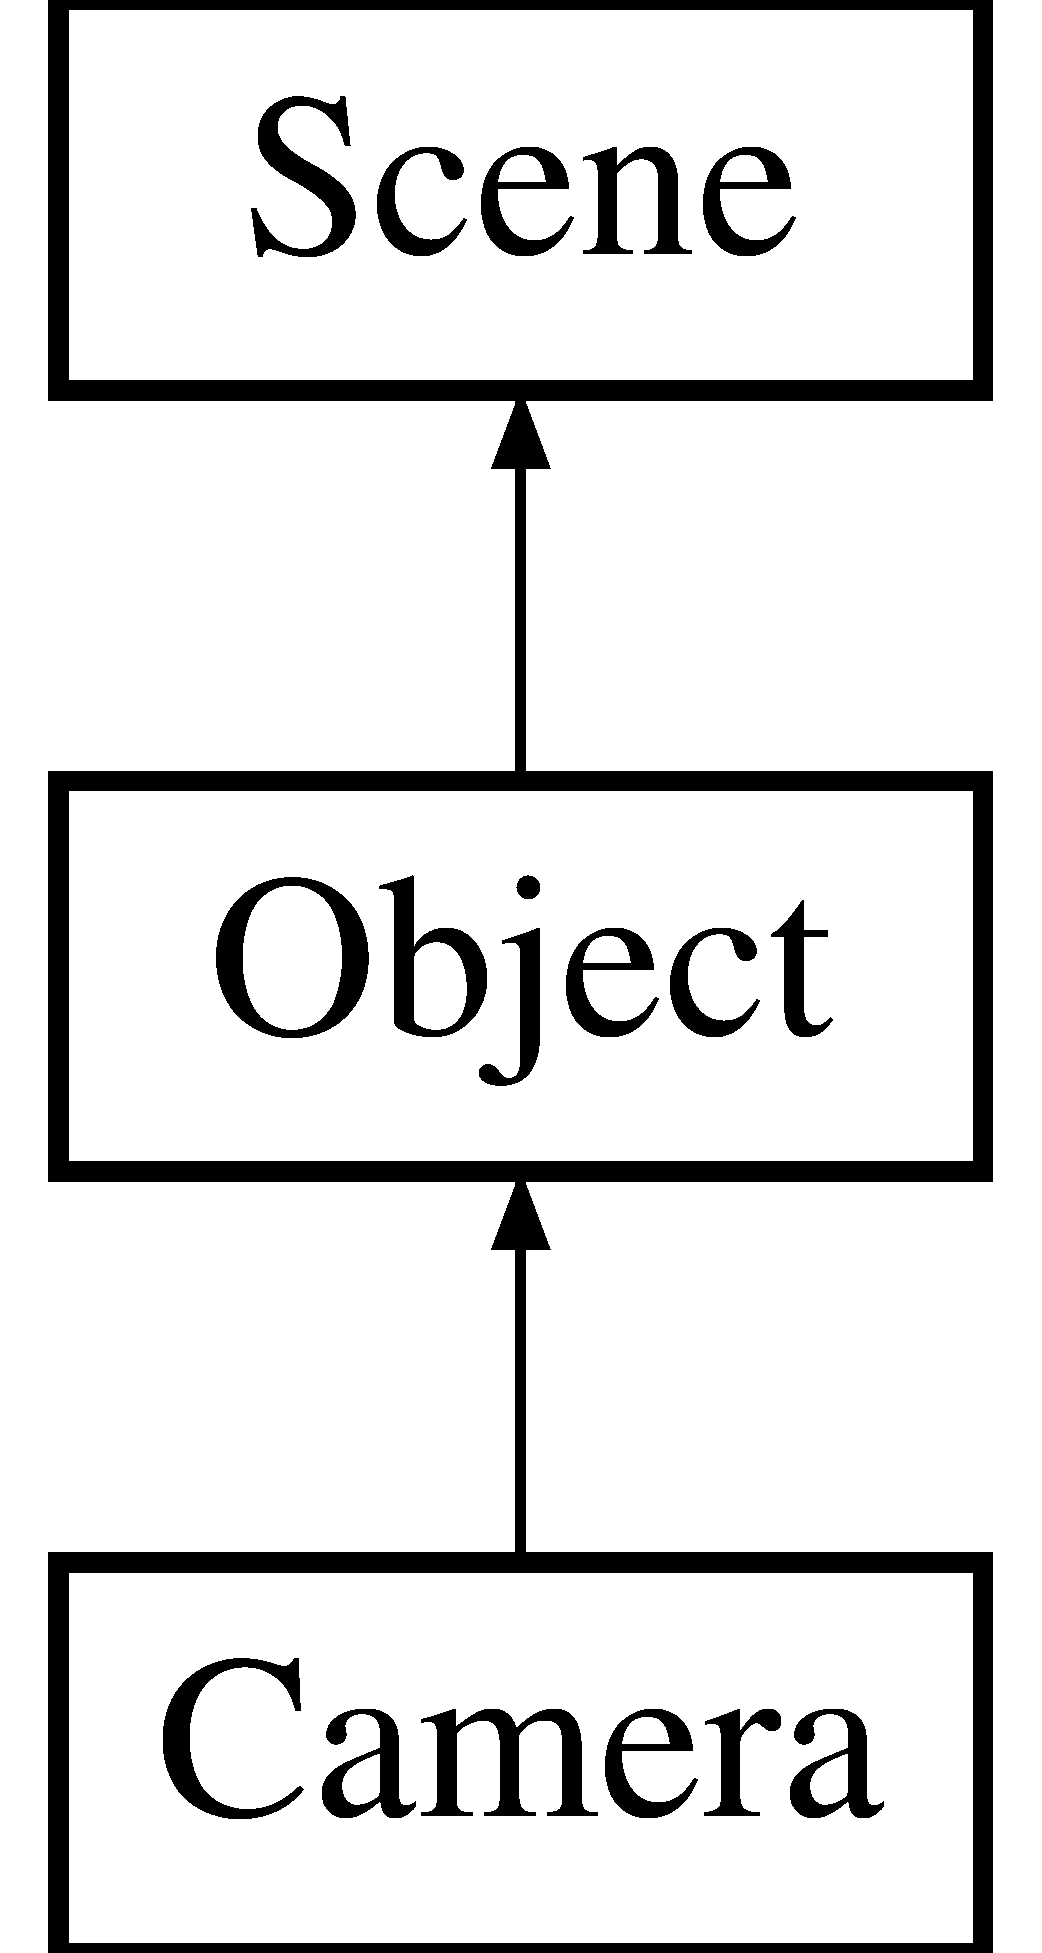
\includegraphics[height=3.000000cm]{class_camera}
\end{center}
\end{figure}
\subsection*{Public Types}
\begin{DoxyCompactItemize}
\item 
enum \hyperlink{class_camera_a80cb65605322d27ad3b6d973484509ec}{Direction} \{ \\*
{\bfseries D\-I\-R\-\_\-\-F\-O\-R\-W\-A\-R\-D}, 
{\bfseries D\-I\-R\-\_\-\-B\-A\-C\-K\-W\-A\-R\-D}, 
{\bfseries D\-I\-R\-\_\-\-L\-E\-F\-T}, 
{\bfseries D\-I\-R\-\_\-\-R\-I\-G\-H\-T}, 
\\*
{\bfseries D\-I\-R\-\_\-\-U\-P}, 
{\bfseries D\-I\-R\-\_\-\-D\-O\-W\-N}, 
{\bfseries D\-I\-R\-\_\-\-E\-N\-D}, 
{\bfseries D\-I\-R\-\_\-\-B\-E\-G\-I\-N} = D\-I\-R\-\_\-\-F\-O\-R\-W\-A\-R\-D
 \}
\begin{DoxyCompactList}\small\item\em The Direction enumeration lists all of the possible directions the camera may travel in. \end{DoxyCompactList}\item 
enum \hyperlink{class_camera_aaa256acd50a2fa143d9f8d9456e2802f}{View\-Type} \{ \\*
{\bfseries P\-E\-R\-S\-P\-E\-C\-T\-I\-V\-E}, 
{\bfseries O\-R\-T\-H\-O}, 
{\bfseries O\-R\-T\-H\-O2\-D}, 
{\bfseries I\-D\-E\-N\-T\-I\-T\-Y}, 
\\*
{\bfseries F\-R\-U\-S\-T\-U\-M}
 \}
\begin{DoxyCompactList}\small\item\em The View\-Type enumeration lists the various possibilities for the current viewing mode that can be switched between. \end{DoxyCompactList}\item 
enum \hyperlink{class_camera_a630738fd23098d44c0d15ee28d5649dd}{Uniforms} \{ \\*
{\bfseries B\-E\-G\-I\-N} = Object\-:\-:E\-N\-D, 
{\bfseries T\-R\-A\-N\-S\-L\-A\-T\-I\-O\-N} = B\-E\-G\-I\-N, 
{\bfseries R\-O\-T\-A\-T\-I\-O\-N}, 
{\bfseries V\-I\-E\-W}, 
\\*
{\bfseries C\-T\-M}, 
{\bfseries E\-N\-D}
 \}
\begin{DoxyCompactList}\small\item\em The glsl\-\_\-var enumeration lists the various variables the \hyperlink{class_camera}{Camera} class is capable of sending to the shader. \end{DoxyCompactList}\item 
typedef enum \hyperlink{class_camera_a80cb65605322d27ad3b6d973484509ec}{Camera\-::\-Direction} \hyperlink{class_camera_a94bb7ceb1c7a05e54cf638924f228baf}{Direction}
\begin{DoxyCompactList}\small\item\em The Direction enumeration lists all of the possible directions the camera may travel in. \end{DoxyCompactList}\item 
typedef enum \hyperlink{class_camera_aaa256acd50a2fa143d9f8d9456e2802f}{Camera\-::\-View\-Type} \hyperlink{class_camera_a5b2dc5eaed6cbaabee0eea3f2714acd7}{View\-Type}
\begin{DoxyCompactList}\small\item\em The View\-Type enumeration lists the various possibilities for the current viewing mode that can be switched between. \end{DoxyCompactList}\item 
typedef enum \hyperlink{class_camera_a630738fd23098d44c0d15ee28d5649dd}{Camera\-::\-Uniforms} \hyperlink{class_camera_a0ed19c96505cbb70625938d1e883af24}{Uniform}
\begin{DoxyCompactList}\small\item\em The glsl\-\_\-var enumeration lists the various variables the \hyperlink{class_camera}{Camera} class is capable of sending to the shader. \end{DoxyCompactList}\item 
\hypertarget{class_object_a79b74057dbc5182b85c9c3ba8480fcf2}{typedef const unsigned int {\bfseries Uniform\-Enum}}\label{class_object_a79b74057dbc5182b85c9c3ba8480fcf2}

\item 
\hypertarget{class_object_a6e19bd8516360bff956408cbae33b878}{typedef std\-::map\\*
$<$ Object\-::\-Uniform\-Enum, \\*
std\-::string $>$ {\bfseries Uniform\-Map}}\label{class_object_a6e19bd8516360bff956408cbae33b878}

\end{DoxyCompactItemize}
\subsection*{Public Member Functions}
\begin{DoxyCompactItemize}
\item 
\hyperlink{class_camera_a16516fa8c830cecef5c8eb43eff12783}{Camera} (const std\-::string \&\hyperlink{class_object_a24457e0a387492c80594aec7681a2277}{name}, G\-Luint g\-Shader, float \hyperlink{class_camera_a14d59ca64bf258adacbed4e0e70ba701}{x}=0.\-0, float \hyperlink{class_camera_a5021b8379a853f306851837178856db0}{y}=0.\-0, float \hyperlink{class_camera_a4acfa20291c83f13c98781c0d53cdbd8}{z}=0.\-0)
\begin{DoxyCompactList}\small\item\em Initialization Constructor; sets the x,y,z coordinates explicitly. \end{DoxyCompactList}\item 
\hyperlink{class_camera_a24329612384948d2b64f78094fe84e75}{Camera} (const std\-::string \&\hyperlink{class_object_a24457e0a387492c80594aec7681a2277}{name}, G\-Luint g\-Shader, \hyperlink{struct_angel_1_1vec3}{vec3} \&in)
\begin{DoxyCompactList}\small\item\em Initialization Constructor, uses a vec3 as its initial coordinates. \end{DoxyCompactList}\item 
\hyperlink{class_camera_aa131bc7f1bad2cc8baea463714c4485d}{Camera} (const std\-::string \&\hyperlink{class_object_a24457e0a387492c80594aec7681a2277}{name}, G\-Luint g\-Shader, \hyperlink{struct_angel_1_1vec4}{vec4} \&in)
\begin{DoxyCompactList}\small\item\em Initialization Constructor, uses a vec4 as its initial coordinates. \end{DoxyCompactList}\item 
virtual \hyperlink{class_camera_a06211f202c145b3ec8253f96e1e654a6}{$\sim$\-Camera} (void)
\begin{DoxyCompactList}\small\item\em Default destructor. \end{DoxyCompactList}\item 
void \hyperlink{class_camera_a14d59ca64bf258adacbed4e0e70ba701}{x} (const float \&in, const bool \&update=true)
\begin{DoxyCompactList}\small\item\em Sets the x coordinate of the camera. \end{DoxyCompactList}\item 
void \hyperlink{class_camera_a5021b8379a853f306851837178856db0}{y} (const float \&in, const bool \&update=true)
\begin{DoxyCompactList}\small\item\em Sets the y coordinate of the camera. \end{DoxyCompactList}\item 
void \hyperlink{class_camera_a4acfa20291c83f13c98781c0d53cdbd8}{z} (const float \&in, const bool \&update=true)
\begin{DoxyCompactList}\small\item\em Sets the z coordinate of the camera. \end{DoxyCompactList}\item 
void \hyperlink{class_camera_a432e03c15d63f8839fe4731016d907a4}{pos} (const float \&\hyperlink{class_camera_a14d59ca64bf258adacbed4e0e70ba701}{x}, const float \&\hyperlink{class_camera_a5021b8379a853f306851837178856db0}{y}, const float \&\hyperlink{class_camera_a4acfa20291c83f13c98781c0d53cdbd8}{z}, const bool \&update=true)
\begin{DoxyCompactList}\small\item\em Sets the absolute position of the camera. \end{DoxyCompactList}\item 
void \hyperlink{class_camera_ae9dc2206b71b25cf320a05d148cb8b56}{pos} (const \hyperlink{struct_angel_1_1vec3}{vec3} \&in, const bool \&update=true)
\begin{DoxyCompactList}\small\item\em Sets the absolute position of the camera. \end{DoxyCompactList}\item 
void \hyperlink{class_camera_aec2115038562e514193bb2b67f5da153}{pos} (const \hyperlink{struct_angel_1_1vec4}{vec4} \&in, const bool \&update=true)
\begin{DoxyCompactList}\small\item\em Sets the absolute position of the camera. \end{DoxyCompactList}\item 
void \hyperlink{class_camera_ac7985a6cb48f4e1e74fda17e5213dd74}{d\-X} (const float \&by, const bool \&update=true)
\begin{DoxyCompactList}\small\item\em Moves the camera along the x axis. \end{DoxyCompactList}\item 
void \hyperlink{class_camera_a59570a88e3ff2d277c9e995372fcadfe}{d\-Y} (const float \&by, const bool \&update=true)
\begin{DoxyCompactList}\small\item\em Moves the camera along the y axis. \end{DoxyCompactList}\item 
void \hyperlink{class_camera_ab94ed9b3c7e12f484d6bfa5f827b59ff}{d\-Z} (const float \&by, const bool \&update=true)
\begin{DoxyCompactList}\small\item\em Moves the camera along the z axis. \end{DoxyCompactList}\item 
void \hyperlink{class_camera_a2ac5f89b4f9f012dead66980925143c0}{d\-Pos} (const float \&\hyperlink{class_camera_a14d59ca64bf258adacbed4e0e70ba701}{x}, const float \&\hyperlink{class_camera_a5021b8379a853f306851837178856db0}{y}, const float \&\hyperlink{class_camera_a4acfa20291c83f13c98781c0d53cdbd8}{z})
\begin{DoxyCompactList}\small\item\em Moves the camera along the x, y, and z axes. \end{DoxyCompactList}\item 
void \hyperlink{class_camera_a928de59670f0b31264307a8a0888b99d}{d\-Pos} (const \hyperlink{struct_angel_1_1vec3}{vec3} \&by)
\begin{DoxyCompactList}\small\item\em Moves the camera along the x, y, and z axes. \end{DoxyCompactList}\item 
void \hyperlink{class_camera_a4ec2e3d2a66826aedb1ac1eee7da0b96}{d\-Pos} (const \hyperlink{struct_angel_1_1vec4}{vec4} \&by)
\begin{DoxyCompactList}\small\item\em Moves the camera along the x, y, and z axes. \end{DoxyCompactList}\item 
void \hyperlink{class_camera_a36ec0e0e832f789e27d42e7bd4f6d174}{field\-Of\-View} (const float \&fovy)
\begin{DoxyCompactList}\small\item\em field\-Of\-View sets the current camera Field-\/of-\/view angle. \end{DoxyCompactList}\item 
float \hyperlink{class_camera_a9b3675bf6866a67f8fa802bb4aecba89}{field\-Of\-View} (void) const 
\begin{DoxyCompactList}\small\item\em \hyperlink{class_camera_a9b3675bf6866a67f8fa802bb4aecba89}{field\-Of\-View()} gets the current camera Field-\/of-\/view angle. \end{DoxyCompactList}\item 
void \hyperlink{class_camera_a717f5d58bb0a73f8c5513a3520d98203}{adjust\-Field\-Of\-View} (const float \&by)
\begin{DoxyCompactList}\small\item\em adjust\-Field\-Of\-View adjusts the field of view angle up or down by an amount. \end{DoxyCompactList}\item 
void \hyperlink{class_camera_a8463a19c9e1e7a1c51cd97051e937230}{change\-Perspective} (const \hyperlink{class_camera_aaa256acd50a2fa143d9f8d9456e2802f}{View\-Type} \&v\-Type)
\begin{DoxyCompactList}\small\item\em change\-Perspective changes the current perspective of the camera. \end{DoxyCompactList}\item 
void \hyperlink{class_camera_a24c5346fc0dfaa93257b6716fe0f2421}{refresh\-Perspective} (void)
\begin{DoxyCompactList}\small\item\em refresh\-Perspective re-\/generates the current view/perspective matrix of the camera. \end{DoxyCompactList}\item 
void \hyperlink{class_camera_adda458a9212825164b52019597f2e9c8}{viewport} (size\-\_\-t \-\_\-\-X, size\-\_\-t \-\_\-\-Y, size\-\_\-t \-\_\-width, size\-\_\-t \-\_\-height)
\begin{DoxyCompactList}\small\item\em viewport instructs this camera what his expected drawing window will be. \end{DoxyCompactList}\item 
void \hyperlink{class_camera_abbe6fe82ed05e64e35b0c4ed2001b34e}{sway} (const float \&by)
\begin{DoxyCompactList}\small\item\em Adjusts the camera's x coordinate relative to its current position. \end{DoxyCompactList}\item 
void \hyperlink{class_camera_abb2251df65445bf8efd3fe0074fb5033}{surge} (const float \&by)
\begin{DoxyCompactList}\small\item\em Adjusts the camera's z coordinate relative to its current position. \end{DoxyCompactList}\item 
void \hyperlink{class_camera_a2148d751f104d8e39c9832e2372df2d9}{heave} (const float \&by)
\begin{DoxyCompactList}\small\item\em Adjusts the camera's y coordinate relative to its current position. \end{DoxyCompactList}\item 
void \hyperlink{class_camera_aac7dbb6201be7f17e014fc6fdf915560}{pitch} (const float \&by, const bool \&fixed=false)
\begin{DoxyCompactList}\small\item\em pitch adjusts the x axis rotation; up/down look. \end{DoxyCompactList}\item 
void \hyperlink{class_camera_a0ce7d12edbe47d9a8915d8af98d8f524}{yaw} (const float \&by, const bool \&fixed=false)
\begin{DoxyCompactList}\small\item\em yaw adjusts the y axis rotation; left/right look. \end{DoxyCompactList}\item 
void \hyperlink{class_camera_a1ba0979fe0b2ec58085d5f9721858e5e}{roll} (const float \&by, const bool \&fixed=false)
\begin{DoxyCompactList}\small\item\em roll adjusts the z axis rotation; tilt or lean left/right. \end{DoxyCompactList}\item 
void \hyperlink{class_camera_aaa9706527438bd5bd323dd018bb34fcf}{move} (const \hyperlink{class_camera_a80cb65605322d27ad3b6d973484509ec}{Camera\-::\-Direction} \&Dir)
\begin{DoxyCompactList}\small\item\em move instructs the camera to begin moving in the specified direction. \end{DoxyCompactList}\item 
void \hyperlink{class_camera_ae7414c6ae83c3c9392ab90e957daf2b9}{stop} (const \hyperlink{class_camera_a80cb65605322d27ad3b6d973484509ec}{Camera\-::\-Direction} \&Dir)
\begin{DoxyCompactList}\small\item\em stop instructs the camera to stop moving in the specified direction. \end{DoxyCompactList}\item 
void \hyperlink{class_camera_a9c620bd05c119791c080e479ee71abc2}{idle} (void)
\begin{DoxyCompactList}\small\item\em idle moves the camera forward in whichever directions it is configured to move in. \end{DoxyCompactList}\item 
void \hyperlink{class_camera_abee6a36602b8044478739cea9221ed41}{accel} (const \hyperlink{struct_angel_1_1vec3}{vec3} \&accel)
\begin{DoxyCompactList}\small\item\em accel takes an input vec2 which represents an acceleration, and applies it to the motion vectors with regards to the maximum acceleration and the maximum speed of the camera. \end{DoxyCompactList}\item 
float \hyperlink{class_camera_ab84abdd525581fbaf0462595d0a087d6}{x} (void) const 
\begin{DoxyCompactList}\small\item\em \hyperlink{class_camera_ab84abdd525581fbaf0462595d0a087d6}{x()} returns the current position of the camera in model coordinates. \end{DoxyCompactList}\item 
float \hyperlink{class_camera_a68d0865ed19510ee41c6477511d70185}{y} (void) const 
\begin{DoxyCompactList}\small\item\em \hyperlink{class_camera_a68d0865ed19510ee41c6477511d70185}{y()} returns the current position of the camera in model coordinates. \end{DoxyCompactList}\item 
float \hyperlink{class_camera_ab1167495c547046c57b1c417e53c39f6}{z} (void) const 
\begin{DoxyCompactList}\small\item\em \hyperlink{class_camera_ab1167495c547046c57b1c417e53c39f6}{z()} returns the current position of the camera in model coordinates. \end{DoxyCompactList}\item 
\hyperlink{struct_angel_1_1vec4}{vec4} \hyperlink{class_camera_a9982ac5f48fe0af97fefa725080d6da6}{pos} (void) const 
\begin{DoxyCompactList}\small\item\em \hyperlink{class_camera_a9982ac5f48fe0af97fefa725080d6da6}{pos()} gets the current camera position in model coordinates. \end{DoxyCompactList}\item 
virtual void \hyperlink{class_camera_a401decef27b59d6485b4ab9762f5b9e6}{send} (Object\-::\-Uniform\-Enum which)
\begin{DoxyCompactList}\small\item\em send will send a glsl variable to the shader. \end{DoxyCompactList}\item 
void \hyperlink{class_camera_ae845a36306bba6b6e359cbdddce65f7f}{view} (void)
\begin{DoxyCompactList}\small\item\em view will instruct Open\-G\-L of the viewport we want, and then send all of our current matrices to the shader for rendering. \end{DoxyCompactList}\item 
void \hyperlink{class_camera_a8ec7938c5e25068e5bff25aeb7038af4}{reset\-Rotation} (void)
\begin{DoxyCompactList}\small\item\em reset\-Rotation adjusts the camera's rotational state back to its default state (The Identity Matrix.) \end{DoxyCompactList}\item 
\hypertarget{class_object_a3afa1b9af32b78d81b5de0836c511aeb}{void {\bfseries Draw} (void)}\label{class_object_a3afa1b9af32b78d81b5de0836c511aeb}

\item 
\hypertarget{class_object_a35c89a8eb8a5b742a9025331119bfc7c}{void {\bfseries Buffer} (void)}\label{class_object_a35c89a8eb8a5b742a9025331119bfc7c}

\item 
\hypertarget{class_object_a754f9f36a528f050b25d053ed43015f0}{void {\bfseries Buffer\-Morph\-Only} (void)}\label{class_object_a754f9f36a528f050b25d053ed43015f0}

\item 
\hypertarget{class_object_ac6ccf69d21c4c902c62829c48ef6cf5b}{void {\bfseries Mode} (G\-Lenum new\-\_\-node)}\label{class_object_ac6ccf69d21c4c902c62829c48ef6cf5b}

\item 
\hypertarget{class_object_aa104adfbcc2cae4bd68c053cc3dab721}{void {\bfseries Texture} (const char $\ast$$\ast$filename)}\label{class_object_aa104adfbcc2cae4bd68c053cc3dab721}

\item 
\hypertarget{class_object_a890760dff9df547454112ff84510040c}{const std\-::string \& {\bfseries Name} (void) const }\label{class_object_a890760dff9df547454112ff84510040c}

\item 
\hypertarget{class_object_accde5aa6e8d0d582719e94c414c2341c}{virtual void {\bfseries Link} (Uniform\-Enum which, const std\-::string \&\hyperlink{class_object_a24457e0a387492c80594aec7681a2277}{name})}\label{class_object_accde5aa6e8d0d582719e94c414c2341c}

\item 
virtual G\-Luint \hyperlink{class_object_a3dc857b837e8b77ba8a2727233400a5e}{Shader} (void)
\begin{DoxyCompactList}\small\item\em Returns the \hyperlink{class_object}{Object}'s current Shader. \end{DoxyCompactList}\item 
virtual void \hyperlink{class_object_aa52c30bca96800cecba55f446e147859}{Shader} (G\-Luint new\-Shader)
\begin{DoxyCompactList}\small\item\em Sets the shader to be used by this object. \end{DoxyCompactList}\item 
\hypertarget{class_object_ae3226b31c80c9f276ffdee65101c8fa6}{void {\bfseries Animation} (void($\ast$anim\-\_\-func)(\hyperlink{class_trans_cache}{Trans\-Cache} \&arg))}\label{class_object_ae3226b31c80c9f276ffdee65101c8fa6}

\item 
\hypertarget{class_object_ae09449132d3853e179d07d4d6bc0b695}{void {\bfseries Propagate} (void)}\label{class_object_ae09449132d3853e179d07d4d6bc0b695}

\item 
\hyperlink{struct_angel_1_1vec4}{vec4} \hyperlink{class_object_ae10497fea640753a3cb63f739aacc540}{Get\-Position} () const 
\begin{DoxyCompactList}\small\item\em returns the position of the object this makes the lighting implementation much easier... \end{DoxyCompactList}\item 
\hypertarget{class_object_aa60771518c07a0edf5aeee5584a571e0}{\hyperlink{class_object}{Object} $\ast$ {\bfseries get\-Morph\-Target\-Ptr} () const }\label{class_object_aa60771518c07a0edf5aeee5584a571e0}

\item 
\hypertarget{class_object_af4d40010633d77ff47e75d40e3129894}{\hyperlink{class_object}{Object} $\ast$ {\bfseries gen\-Morph\-Target} (G\-Luint)}\label{class_object_af4d40010633d77ff47e75d40e3129894}

\item 
\hypertarget{class_object_a275903685e300433a5120b5558eb9aa1}{float {\bfseries get\-Morph\-Percentage} () const }\label{class_object_a275903685e300433a5120b5558eb9aa1}

\item 
\hypertarget{class_object_aea00114a91aeb779b4f03c7bebaa326e}{void {\bfseries set\-Morph\-Percentage} (const float)}\label{class_object_aea00114a91aeb779b4f03c7bebaa326e}

\item 
\hypertarget{class_object_a98d3f1b9ebb61c3b21e2a59ed267480a}{void {\bfseries destroy\-Morph\-Target} ()}\label{class_object_a98d3f1b9ebb61c3b21e2a59ed267480a}

\item 
\hypertarget{class_object_aae9b55b35a69ba78aa2803b4c8a681b7}{int {\bfseries get\-Number\-Points} ()}\label{class_object_aae9b55b35a69ba78aa2803b4c8a681b7}

\item 
\hypertarget{class_scene_a366b5dec1ecf66a887b4d0dedcd1aa3b}{\hyperlink{class_object}{Object} $\ast$ {\bfseries Add\-Object} (const std\-::string \&obj\-Name, G\-Luint Object\-\_\-\-Shader=0)}\label{class_scene_a366b5dec1ecf66a887b4d0dedcd1aa3b}

\item 
\hypertarget{class_scene_a3bd9fa1058f506c04162b9283e97d20e}{void {\bfseries Del\-Object} (const std\-::string \&obj\-Name)}\label{class_scene_a3bd9fa1058f506c04162b9283e97d20e}

\item 
\hypertarget{class_scene_a43fd3c56db5dc940d1724b9573c9a360}{void {\bfseries Del\-Object} (void)}\label{class_scene_a43fd3c56db5dc940d1724b9573c9a360}

\item 
\hypertarget{class_scene_abdfd15e7987aa261840d5ecc265170df}{void {\bfseries Pop\-Object} (void)}\label{class_scene_abdfd15e7987aa261840d5ecc265170df}

\item 
\hypertarget{class_scene_a82759ded1f6f87a91b8d10ed87501958}{void \hyperlink{class_scene_a82759ded1f6f87a91b8d10ed87501958}{Destroy\-Object} (void)}\label{class_scene_a82759ded1f6f87a91b8d10ed87501958}

\begin{DoxyCompactList}\small\item\em Completely remove this object and all his children. \end{DoxyCompactList}\item 
\hypertarget{class_scene_a70fcdad192a4c6ff508125de8af6cf4d}{\hyperlink{class_object}{Object} $\ast$ {\bfseries next} (void)}\label{class_scene_a70fcdad192a4c6ff508125de8af6cf4d}

\item 
\hypertarget{class_scene_ac852d5d763eb35b4908c9aa7ea54d1ae}{\hyperlink{class_object}{Object} $\ast$ {\bfseries prev} (void)}\label{class_scene_ac852d5d763eb35b4908c9aa7ea54d1ae}

\item 
\hypertarget{class_scene_ad0ea1a6bcf7815c63988bd937f06eb23}{\hyperlink{class_object}{Object} $\ast$ {\bfseries active} (void) const }\label{class_scene_ad0ea1a6bcf7815c63988bd937f06eb23}

\item 
\hypertarget{class_scene_ae9b69d8db8a46991017635f22e45baad}{\hyperlink{class_object}{Object} $\ast$ {\bfseries operator\mbox{[}$\,$\mbox{]}} (const std\-::string \&objname)}\label{class_scene_ae9b69d8db8a46991017635f22e45baad}

\end{DoxyCompactItemize}
\subsection*{Public Attributes}
\begin{DoxyCompactItemize}
\item 
\hypertarget{class_object_a8dec70177d147f59ba10c9eba8e9191b}{std\-::vector$<$ \hyperlink{struct_angel_1_1vec4}{Angel\-::vec4} $>$ {\bfseries points}}\label{class_object_a8dec70177d147f59ba10c9eba8e9191b}

\item 
\hypertarget{class_object_ad541a7bb180e24f59d752cc6d7f8c7e8}{std\-::vector$<$ \hyperlink{struct_angel_1_1vec3}{Angel\-::vec3} $>$ {\bfseries normals}}\label{class_object_ad541a7bb180e24f59d752cc6d7f8c7e8}

\item 
\hypertarget{class_object_a9b2fb19d129ad79407f9af0eea05b96c}{std\-::vector$<$ unsigned int $>$ {\bfseries indices}}\label{class_object_a9b2fb19d129ad79407f9af0eea05b96c}

\item 
\hypertarget{class_object_a4de4c1e2c4b621efb6f5d1b398ac6835}{std\-::vector$<$ \hyperlink{struct_angel_1_1vec4}{Angel\-::vec4} $>$ {\bfseries colors}}\label{class_object_a4de4c1e2c4b621efb6f5d1b398ac6835}

\item 
\hypertarget{class_object_a6d6c58ccb93f7a2bd7439d081134aaa0}{std\-::vector$<$ \hyperlink{struct_angel_1_1vec2}{Angel\-::vec2} $>$ {\bfseries texcoords}}\label{class_object_a6d6c58ccb93f7a2bd7439d081134aaa0}

\item 
\hypertarget{class_object_a1bb011587e4fa6e69984d5679546b1cb}{\hyperlink{class_trans_cache}{Trans\-Cache} {\bfseries trans}}\label{class_object_a1bb011587e4fa6e69984d5679546b1cb}

\end{DoxyCompactItemize}
\subsection*{Protected Member Functions}
\begin{DoxyCompactItemize}
\item 
void \hyperlink{class_scene_a8bbe0e5b1bfc71034b18e240e86aa285}{Delete\-Object} (\hyperlink{class_object}{Object} $\ast$obj)
\begin{DoxyCompactList}\small\item\em Delete\-Object is the actual implementation function that will remove an \hyperlink{class_object}{Object} from the \hyperlink{class_scene}{Scene} list and \hyperlink{class_scene}{Scene} map, then free the object. \end{DoxyCompactList}\item 
\hypertarget{class_scene_ae8d51ddc196248a7cbd1f3640851dbd4}{void {\bfseries Insert\-Object} (const std\-::string \hyperlink{class_object_a24457e0a387492c80594aec7681a2277}{name}, \hyperlink{class_object}{Object} $\ast$obj)}\label{class_scene_ae8d51ddc196248a7cbd1f3640851dbd4}

\end{DoxyCompactItemize}
\subsection*{Protected Attributes}
\begin{DoxyCompactItemize}
\item 
std\-::string \hyperlink{class_object_a24457e0a387492c80594aec7681a2277}{name}
\begin{DoxyCompactList}\small\item\em name is used as an identifying handle for the object. \end{DoxyCompactList}\item 
G\-Luint \hyperlink{class_object_a66190fee29d03d6478516686cbd01eb8}{vao}
\begin{DoxyCompactList}\small\item\em Vertex Array \hyperlink{class_object}{Object} handle identifying our buffers/object. \end{DoxyCompactList}\item 
\hypertarget{class_object_a29de966ce95d96e19262c4f10f0b4276}{G\-Luint \hyperlink{class_object_a29de966ce95d96e19262c4f10f0b4276}{buffer} \mbox{[}N\-U\-M\-\_\-\-B\-U\-F\-F\-E\-R\-S\mbox{]}}\label{class_object_a29de966ce95d96e19262c4f10f0b4276}

\begin{DoxyCompactList}\small\item\em Handles to our buffers (Vertices, Tex\-U\-Vs, etc.) \end{DoxyCompactList}\item 
G\-Lenum \hyperlink{class_object_a82764b385767d989f27d301ab206acb8}{draw\-\_\-mode}
\begin{DoxyCompactList}\small\item\em Drawing mode for this object. \end{DoxyCompactList}\item 
\hypertarget{class_object_a2bbbe3a5b33cbcfc4c536b49d470a6b8}{bool \hyperlink{class_object_a2bbbe3a5b33cbcfc4c536b49d470a6b8}{is\-Textured}}\label{class_object_a2bbbe3a5b33cbcfc4c536b49d470a6b8}

\begin{DoxyCompactList}\small\item\em Is this object textured? \end{DoxyCompactList}\item 
\hypertarget{class_object_ac5ca00d03136434b93ae7d00808554c7}{float \hyperlink{class_object_ac5ca00d03136434b93ae7d00808554c7}{morph\-Percentage}}\label{class_object_ac5ca00d03136434b93ae7d00808554c7}

\begin{DoxyCompactList}\small\item\em Morphing/\-Tweening Things. \end{DoxyCompactList}\item 
\hypertarget{class_object_acfc4dec49d5d273910c3a1af2b3adfcd}{\hyperlink{class_object}{Object} $\ast$ {\bfseries morph\-Target}}\label{class_object_acfc4dec49d5d273910c3a1af2b3adfcd}

\item 
\hypertarget{class_object_a6378d0b0eeec23045ae2a5245e42bf13}{std\-::map$<$ Object\-::\-Uniform\-Enum, \\*
std\-::string $>$ {\bfseries \-\_\-uniform\-Map}}\label{class_object_a6378d0b0eeec23045ae2a5245e42bf13}

\item 
std\-::vector$<$ G\-Lint $>$ \hyperlink{class_object_acd6c7021617ea334915a1525f9519bc5}{handles}
\begin{DoxyCompactList}\small\item\em Handles to Uniforms on the shader. \end{DoxyCompactList}\item 
\hypertarget{class_scene_acdd0123ca6b2d64d8d447bb485b235fc}{std\-::list$<$ \hyperlink{class_object}{Object} $\ast$ $>$ {\bfseries \-\_\-list}}\label{class_scene_acdd0123ca6b2d64d8d447bb485b235fc}

\item 
\hypertarget{class_scene_a8bd5d86484a12255b26b92b6cbf8d29a}{std\-::map$<$ std\-::string, \hyperlink{class_object}{Object} $\ast$ $>$ {\bfseries \-\_\-map}}\label{class_scene_a8bd5d86484a12255b26b92b6cbf8d29a}

\item 
\hypertarget{class_scene_ae87ca5350fcc595f3f15a4fd3c39f3d9}{std\-::list$<$ \hyperlink{class_object}{Object} $\ast$ $>$\-::iterator {\bfseries \-\_\-current\-Obj}}\label{class_scene_ae87ca5350fcc595f3f15a4fd3c39f3d9}

\item 
\hypertarget{class_scene_a8f9bdd8ec5edb1f414fbd314a36e2724}{G\-Luint {\bfseries \-\_\-g\-Shader}}\label{class_scene_a8f9bdd8ec5edb1f414fbd314a36e2724}

\end{DoxyCompactItemize}
\subsection*{Private Member Functions}
\begin{DoxyCompactItemize}
\item 
void \hyperlink{class_camera_aba32f195cdb5bfcfd05c2ce74315b6c3}{adjust\-Rotation} (const \hyperlink{class_angel_1_1mat4}{mat4} \&adjustment, const bool \&fixed=false)
\begin{DoxyCompactList}\small\item\em adjust\-Rotation is an internal function that rotates the camera. \end{DoxyCompactList}\item 
void \hyperlink{class_camera_a20243a7e3eb06ab1265118c5fb9cce9b}{common\-Init} (void)
\begin{DoxyCompactList}\small\item\em common\-Init is a private function that initializes local object attributes. \end{DoxyCompactList}\end{DoxyCompactItemize}
\subsection*{Private Attributes}
\begin{DoxyCompactItemize}
\item 
\hyperlink{class_angel_1_1mat4}{mat4} \hyperlink{class_camera_a28f6e710df6db726568cd0f2bbd3643a}{\-\_\-view}
\begin{DoxyCompactList}\small\item\em The current view matrix (defaultly perspective) for this camera. \end{DoxyCompactList}\item 
\hyperlink{class_trans_cache}{Trans\-Cache} \hyperlink{class_camera_a6c1e31c8470b923f9f872f73597cb95b}{\-\_\-ctm}
\begin{DoxyCompactList}\small\item\em The Current \hyperlink{class_transformation}{Transformation} state for this \hyperlink{class_camera}{Camera}. \end{DoxyCompactList}\item 
\hyperlink{class_camera_aaa256acd50a2fa143d9f8d9456e2802f}{View\-Type} \hyperlink{class_camera_ac9062d9bb891aa81d163076738451081}{\-\_\-current\-View}
\begin{DoxyCompactList}\small\item\em The current viewing mode type. \end{DoxyCompactList}\item 
G\-Lfloat \hyperlink{class_camera_a21f8eb53e5369018e39add0453ae626d}{\-\_\-speed}
\begin{DoxyCompactList}\small\item\em Current Speed of camera motion. \end{DoxyCompactList}\item 
\hyperlink{struct_angel_1_1vec3}{vec3} \hyperlink{class_camera_aa15577ff9e67c81699ee86d4d20a7ee7}{\-\_\-velocity}
\begin{DoxyCompactList}\small\item\em Current Velocity of camera motion. \end{DoxyCompactList}\item 
\hypertarget{class_camera_a4d875d29a43bdfed4eac4c76747939d3}{G\-Lfloat \hyperlink{class_camera_a4d875d29a43bdfed4eac4c76747939d3}{\-\_\-speed\-\_\-cap}}\label{class_camera_a4d875d29a43bdfed4eac4c76747939d3}

\begin{DoxyCompactList}\small\item\em Current Speed Capacity\-: (speed/\-Max\-Speed) \end{DoxyCompactList}\item 
\hypertarget{class_camera_acbfae99c73c118ca92be9a6ba664b303}{G\-Lfloat \hyperlink{class_camera_acbfae99c73c118ca92be9a6ba664b303}{\-\_\-max\-Accel}}\label{class_camera_acbfae99c73c118ca92be9a6ba664b303}

\begin{DoxyCompactList}\small\item\em Maximum Acceleration Magnitude. \end{DoxyCompactList}\item 
\hypertarget{class_camera_a83cab43f9ccc3d5f4c7db8543a806745}{G\-Lfloat \hyperlink{class_camera_a83cab43f9ccc3d5f4c7db8543a806745}{\-\_\-max\-Speed}}\label{class_camera_a83cab43f9ccc3d5f4c7db8543a806745}

\begin{DoxyCompactList}\small\item\em Maximum Speed. \end{DoxyCompactList}\item 
G\-Lfloat \hyperlink{class_camera_a66fb66da0ccd400c4986dc19276b6716}{\-\_\-friction\-Magnitude}
\begin{DoxyCompactList}\small\item\em Friction. \end{DoxyCompactList}\item 
G\-Lfloat \hyperlink{class_camera_a42082e8f2d80a13674ce163d8e720bfb}{\-\_\-aspect\-Ratio}
\begin{DoxyCompactList}\small\item\em Current aspect ratio for certain perspectives. \end{DoxyCompactList}\item 
G\-Lfloat \hyperlink{class_camera_a82542bb76347e2a2bb66b3bb7842945b}{\-\_\-fovy}
\begin{DoxyCompactList}\small\item\em Current field-\/of-\/view angle for perspective view. \end{DoxyCompactList}\item 
\hypertarget{class_camera_a67c7600162abef1d2cddfce8cc75c33b}{\hyperlink{struct_angel_1_1vec2}{Angel\-::vec2} \hyperlink{class_camera_a67c7600162abef1d2cddfce8cc75c33b}{\-\_\-viewport\-Size}}\label{class_camera_a67c7600162abef1d2cddfce8cc75c33b}

\begin{DoxyCompactList}\small\item\em \hyperlink{class_camera}{Camera}'s Drawbox Width and Height. \end{DoxyCompactList}\item 
\hypertarget{class_camera_adb7506be3632abc2d33e77a5783f5be8}{\hyperlink{struct_angel_1_1vec2}{Angel\-::vec2} \hyperlink{class_camera_adb7506be3632abc2d33e77a5783f5be8}{\-\_\-viewport\-Position}}\label{class_camera_adb7506be3632abc2d33e77a5783f5be8}

\begin{DoxyCompactList}\small\item\em \hyperlink{class_camera}{Camera}'s Drawbox x,y Coordinate (Upper-\/\-Left Pixel) \end{DoxyCompactList}\item 
bool \hyperlink{class_camera_abec7e2becbad5a692a54a69b6a5f6d75}{\-\_\-motion} \mbox{[}Camera\-::\-D\-I\-R\-\_\-\-E\-N\-D\mbox{]}
\begin{DoxyCompactList}\small\item\em Booleans correlating to the different motion directions. \end{DoxyCompactList}\end{DoxyCompactItemize}


\subsection{Detailed Description}
The \hyperlink{class_camera}{Camera} class represents a logical camera in a model view, which posesses a current viewing angle and an absolute position in space as its state. 

\begin{DoxyAuthor}{Author}
John Huston, \href{mailto:jhuston@cs.uml.edu}{\tt jhuston@cs.\-uml.\-edu} 
\end{DoxyAuthor}
\begin{DoxySince}{Since}
16 Nov 2012
\end{DoxySince}
Functions are provided to adjust the rotation according to \hyperlink{class_camera_aac7dbb6201be7f17e014fc6fdf915560}{pitch()}, \hyperlink{class_camera_a0ce7d12edbe47d9a8915d8af98d8f524}{yaw()} and \hyperlink{class_camera_a1ba0979fe0b2ec58085d5f9721858e5e}{roll()} motions; \hyperlink{class_camera_abb2251df65445bf8efd3fe0074fb5033}{surge()}, \hyperlink{class_camera_abbe6fe82ed05e64e35b0c4ed2001b34e}{sway()}, and \hyperlink{class_camera_a2148d751f104d8e39c9832e2372df2d9}{heave()} are provided to adjust position in space.

\hyperlink{class_camera_aaa9706527438bd5bd323dd018bb34fcf}{move()}, \hyperlink{class_camera_ae7414c6ae83c3c9392ab90e957daf2b9}{stop()}, and \hyperlink{class_camera_a9c620bd05c119791c080e479ee71abc2}{idle()} are provided to help the camera automatically move along the x, y, or z axes. 

Definition at line 37 of file Camera.\-hpp.



\subsection{Member Typedef Documentation}
\hypertarget{class_camera_a94bb7ceb1c7a05e54cf638924f228baf}{\index{Camera@{Camera}!Direction@{Direction}}
\index{Direction@{Direction}!Camera@{Camera}}
\subsubsection[{Direction}]{\setlength{\rightskip}{0pt plus 5cm}typedef enum {\bf Camera\-::\-Direction}  {\bf Camera\-::\-Direction}}}\label{class_camera_a94bb7ceb1c7a05e54cf638924f228baf}


The Direction enumeration lists all of the possible directions the camera may travel in. 

'B\-E\-G\-I\-N' and 'E\-N\-D' are special sentinel directions for the purposes of iteration, and are ignored by any functions that accept a Direction. \hypertarget{class_camera_a0ed19c96505cbb70625938d1e883af24}{\index{Camera@{Camera}!Uniform@{Uniform}}
\index{Uniform@{Uniform}!Camera@{Camera}}
\subsubsection[{Uniform}]{\setlength{\rightskip}{0pt plus 5cm}typedef enum {\bf Camera\-::\-Uniforms}  {\bf Camera\-::\-Uniform}}}\label{class_camera_a0ed19c96505cbb70625938d1e883af24}


The glsl\-\_\-var enumeration lists the various variables the \hyperlink{class_camera}{Camera} class is capable of sending to the shader. 

The Num\-Glsl\-Vars variable is a sentinel value that is ignored by any functions that accept a glsl\-\_\-var. \hypertarget{class_camera_a5b2dc5eaed6cbaabee0eea3f2714acd7}{\index{Camera@{Camera}!View\-Type@{View\-Type}}
\index{View\-Type@{View\-Type}!Camera@{Camera}}
\subsubsection[{View\-Type}]{\setlength{\rightskip}{0pt plus 5cm}typedef enum {\bf Camera\-::\-View\-Type}  {\bf Camera\-::\-View\-Type}}}\label{class_camera_a5b2dc5eaed6cbaabee0eea3f2714acd7}


The View\-Type enumeration lists the various possibilities for the current viewing mode that can be switched between. 

The default is P\-E\-R\-S\-P\-E\-C\-T\-I\-V\-E. 

\subsection{Member Enumeration Documentation}
\hypertarget{class_camera_a80cb65605322d27ad3b6d973484509ec}{\index{Camera@{Camera}!Direction@{Direction}}
\index{Direction@{Direction}!Camera@{Camera}}
\subsubsection[{Direction}]{\setlength{\rightskip}{0pt plus 5cm}enum {\bf Camera\-::\-Direction}}}\label{class_camera_a80cb65605322d27ad3b6d973484509ec}


The Direction enumeration lists all of the possible directions the camera may travel in. 

'B\-E\-G\-I\-N' and 'E\-N\-D' are special sentinel directions for the purposes of iteration, and are ignored by any functions that accept a Direction. 

Definition at line 47 of file Camera.\-hpp.

\hypertarget{class_camera_a630738fd23098d44c0d15ee28d5649dd}{\index{Camera@{Camera}!Uniforms@{Uniforms}}
\index{Uniforms@{Uniforms}!Camera@{Camera}}
\subsubsection[{Uniforms}]{\setlength{\rightskip}{0pt plus 5cm}enum {\bf Camera\-::\-Uniforms}}}\label{class_camera_a630738fd23098d44c0d15ee28d5649dd}


The glsl\-\_\-var enumeration lists the various variables the \hyperlink{class_camera}{Camera} class is capable of sending to the shader. 

The Num\-Glsl\-Vars variable is a sentinel value that is ignored by any functions that accept a glsl\-\_\-var. 

Definition at line 73 of file Camera.\-hpp.

\hypertarget{class_camera_aaa256acd50a2fa143d9f8d9456e2802f}{\index{Camera@{Camera}!View\-Type@{View\-Type}}
\index{View\-Type@{View\-Type}!Camera@{Camera}}
\subsubsection[{View\-Type}]{\setlength{\rightskip}{0pt plus 5cm}enum {\bf Camera\-::\-View\-Type}}}\label{class_camera_aaa256acd50a2fa143d9f8d9456e2802f}


The View\-Type enumeration lists the various possibilities for the current viewing mode that can be switched between. 

The default is P\-E\-R\-S\-P\-E\-C\-T\-I\-V\-E. 

Definition at line 63 of file Camera.\-hpp.



\subsection{Constructor \& Destructor Documentation}
\hypertarget{class_camera_a16516fa8c830cecef5c8eb43eff12783}{\index{Camera@{Camera}!Camera@{Camera}}
\index{Camera@{Camera}!Camera@{Camera}}
\subsubsection[{Camera}]{\setlength{\rightskip}{0pt plus 5cm}Camera\-::\-Camera (
\begin{DoxyParamCaption}
\item[{const std\-::string \&}]{name, }
\item[{G\-Luint}]{g\-Shader, }
\item[{float}]{x = {\ttfamily 0.0}, }
\item[{float}]{y = {\ttfamily 0.0}, }
\item[{float}]{z = {\ttfamily 0.0}}
\end{DoxyParamCaption}
)}}\label{class_camera_a16516fa8c830cecef5c8eb43eff12783}


Initialization Constructor; sets the x,y,z coordinates explicitly. 


\begin{DoxyParams}{Parameters}
{\em name} & The name of this Camera/\-Object. \\
\hline
{\em g\-Shader} & A handle to this camera's associated shader object. \\
\hline
{\em x} & The initial x coordinate. \\
\hline
{\em y} & The initial y coordinate. \\
\hline
{\em z} & The initial z coordinate. \\
\hline
\end{DoxyParams}


Definition at line 45 of file Camera.\-cpp.

\hypertarget{class_camera_a24329612384948d2b64f78094fe84e75}{\index{Camera@{Camera}!Camera@{Camera}}
\index{Camera@{Camera}!Camera@{Camera}}
\subsubsection[{Camera}]{\setlength{\rightskip}{0pt plus 5cm}Camera\-::\-Camera (
\begin{DoxyParamCaption}
\item[{const std\-::string \&}]{name, }
\item[{G\-Luint}]{g\-Shader, }
\item[{{\bf vec3} \&}]{in}
\end{DoxyParamCaption}
)}}\label{class_camera_a24329612384948d2b64f78094fe84e75}


Initialization Constructor, uses a vec3 as its initial coordinates. 


\begin{DoxyParams}{Parameters}
{\em name} & The name of this Camera/\-Object. \\
\hline
{\em g\-Shader} & A handle to this camera's associated shader object. \\
\hline
{\em in} & A vec3 representing the initial coordinates. \\
\hline
\end{DoxyParams}


Definition at line 52 of file Camera.\-cpp.

\hypertarget{class_camera_aa131bc7f1bad2cc8baea463714c4485d}{\index{Camera@{Camera}!Camera@{Camera}}
\index{Camera@{Camera}!Camera@{Camera}}
\subsubsection[{Camera}]{\setlength{\rightskip}{0pt plus 5cm}Camera\-::\-Camera (
\begin{DoxyParamCaption}
\item[{const std\-::string \&}]{name, }
\item[{G\-Luint}]{g\-Shader, }
\item[{{\bf vec4} \&}]{in}
\end{DoxyParamCaption}
)}}\label{class_camera_aa131bc7f1bad2cc8baea463714c4485d}


Initialization Constructor, uses a vec4 as its initial coordinates. 


\begin{DoxyParams}{Parameters}
{\em name} & The name of this Camera/\-Object. \\
\hline
{\em g\-Shader} & A handle to this camera's associated shader object. \\
\hline
{\em in} & A vec4 representing the initial coordinates. The w component is ignored. \\
\hline
\end{DoxyParams}


Definition at line 58 of file Camera.\-cpp.

\hypertarget{class_camera_a06211f202c145b3ec8253f96e1e654a6}{\index{Camera@{Camera}!$\sim$\-Camera@{$\sim$\-Camera}}
\index{$\sim$\-Camera@{$\sim$\-Camera}!Camera@{Camera}}
\subsubsection[{$\sim$\-Camera}]{\setlength{\rightskip}{0pt plus 5cm}Camera\-::$\sim$\-Camera (
\begin{DoxyParamCaption}
\item[{void}]{}
\end{DoxyParamCaption}
)\hspace{0.3cm}{\ttfamily [virtual]}}}\label{class_camera_a06211f202c145b3ec8253f96e1e654a6}


Default destructor. 

Defined only to allow inheritance. 

Definition at line 64 of file Camera.\-cpp.



\subsection{Member Function Documentation}
\hypertarget{class_camera_abee6a36602b8044478739cea9221ed41}{\index{Camera@{Camera}!accel@{accel}}
\index{accel@{accel}!Camera@{Camera}}
\subsubsection[{accel}]{\setlength{\rightskip}{0pt plus 5cm}void Camera\-::accel (
\begin{DoxyParamCaption}
\item[{const {\bf vec3} \&}]{accel}
\end{DoxyParamCaption}
)}}\label{class_camera_abee6a36602b8044478739cea9221ed41}


accel takes an input vec2 which represents an acceleration, and applies it to the motion vectors with regards to the maximum acceleration and the maximum speed of the camera. 


\begin{DoxyParams}{Parameters}
{\em accel} & The vec3 which represents the (x,y,z) acceleration, where x,y,z are \mbox{[}-\/1,1\mbox{]}. \\
\hline
\end{DoxyParams}
\begin{DoxyReturn}{Returns}
Void. 
\end{DoxyReturn}


Definition at line 223 of file Camera.\-cpp.

\hypertarget{class_camera_a717f5d58bb0a73f8c5513a3520d98203}{\index{Camera@{Camera}!adjust\-Field\-Of\-View@{adjust\-Field\-Of\-View}}
\index{adjust\-Field\-Of\-View@{adjust\-Field\-Of\-View}!Camera@{Camera}}
\subsubsection[{adjust\-Field\-Of\-View}]{\setlength{\rightskip}{0pt plus 5cm}void Camera\-::adjust\-Field\-Of\-View (
\begin{DoxyParamCaption}
\item[{const float \&}]{by}
\end{DoxyParamCaption}
)}}\label{class_camera_a717f5d58bb0a73f8c5513a3520d98203}


adjust\-Field\-Of\-View adjusts the field of view angle up or down by an amount. 


\begin{DoxyParams}{Parameters}
{\em by} & The float to adjust the field\-Of\-View angle by. \\
\hline
\end{DoxyParams}
\begin{DoxyReturn}{Returns}
Void. 
\end{DoxyReturn}


Definition at line 392 of file Camera.\-cpp.

\hypertarget{class_camera_aba32f195cdb5bfcfd05c2ce74315b6c3}{\index{Camera@{Camera}!adjust\-Rotation@{adjust\-Rotation}}
\index{adjust\-Rotation@{adjust\-Rotation}!Camera@{Camera}}
\subsubsection[{adjust\-Rotation}]{\setlength{\rightskip}{0pt plus 5cm}void Camera\-::adjust\-Rotation (
\begin{DoxyParamCaption}
\item[{const {\bf mat4} \&}]{adjustment, }
\item[{const bool \&}]{fixed = {\ttfamily false}}
\end{DoxyParamCaption}
)\hspace{0.3cm}{\ttfamily [private]}}}\label{class_camera_aba32f195cdb5bfcfd05c2ce74315b6c3}


adjust\-Rotation is an internal function that rotates the camera. 

Technically, any transformation, not just a rotation, is possible. 
\begin{DoxyParams}{Parameters}
{\em adjustment} & The 4x4 matrix to transform the C\-T\-M by. \\
\hline
{\em fixed} & Should this rotation be fixed about the origin? \\
\hline
\end{DoxyParams}
\begin{DoxyReturn}{Returns}
Void. 
\end{DoxyReturn}


Definition at line 148 of file Camera.\-cpp.

\hypertarget{class_camera_a8463a19c9e1e7a1c51cd97051e937230}{\index{Camera@{Camera}!change\-Perspective@{change\-Perspective}}
\index{change\-Perspective@{change\-Perspective}!Camera@{Camera}}
\subsubsection[{change\-Perspective}]{\setlength{\rightskip}{0pt plus 5cm}void Camera\-::change\-Perspective (
\begin{DoxyParamCaption}
\item[{const {\bf View\-Type} \&}]{v\-Type}
\end{DoxyParamCaption}
)}}\label{class_camera_a8463a19c9e1e7a1c51cd97051e937230}


change\-Perspective changes the current perspective of the camera. 


\begin{DoxyParams}{Parameters}
{\em v\-Type} & Which perspective to use. see enum View\-Type for possibilities. \\
\hline
\end{DoxyParams}
\begin{DoxyReturn}{Returns}
Void. 
\end{DoxyReturn}


Definition at line 359 of file Camera.\-cpp.

\hypertarget{class_camera_a20243a7e3eb06ab1265118c5fb9cce9b}{\index{Camera@{Camera}!common\-Init@{common\-Init}}
\index{common\-Init@{common\-Init}!Camera@{Camera}}
\subsubsection[{common\-Init}]{\setlength{\rightskip}{0pt plus 5cm}void Camera\-::common\-Init (
\begin{DoxyParamCaption}
\item[{void}]{}
\end{DoxyParamCaption}
)\hspace{0.3cm}{\ttfamily [private]}}}\label{class_camera_a20243a7e3eb06ab1265118c5fb9cce9b}


common\-Init is a private function that initializes local object attributes. 

It should be called by all available constructors. \begin{DoxyReturn}{Returns}
Void. 
\end{DoxyReturn}


Definition at line 19 of file Camera.\-cpp.

\hypertarget{class_scene_a8bbe0e5b1bfc71034b18e240e86aa285}{\index{Camera@{Camera}!Delete\-Object@{Delete\-Object}}
\index{Delete\-Object@{Delete\-Object}!Camera@{Camera}}
\subsubsection[{Delete\-Object}]{\setlength{\rightskip}{0pt plus 5cm}void Scene\-::\-Delete\-Object (
\begin{DoxyParamCaption}
\item[{{\bf Object} $\ast$}]{obj}
\end{DoxyParamCaption}
)\hspace{0.3cm}{\ttfamily [protected]}, {\ttfamily [inherited]}}}\label{class_scene_a8bbe0e5b1bfc71034b18e240e86aa285}


Delete\-Object is the actual implementation function that will remove an \hyperlink{class_object}{Object} from the \hyperlink{class_scene}{Scene} list and \hyperlink{class_scene}{Scene} map, then free the object. 


\begin{DoxyParams}{Parameters}
{\em obj} & The pointer to the object to free. \\
\hline
\end{DoxyParams}


Definition at line 76 of file Scene.\-cpp.

\hypertarget{class_camera_a2ac5f89b4f9f012dead66980925143c0}{\index{Camera@{Camera}!d\-Pos@{d\-Pos}}
\index{d\-Pos@{d\-Pos}!Camera@{Camera}}
\subsubsection[{d\-Pos}]{\setlength{\rightskip}{0pt plus 5cm}void Camera\-::d\-Pos (
\begin{DoxyParamCaption}
\item[{const float \&}]{x, }
\item[{const float \&}]{y, }
\item[{const float \&}]{z}
\end{DoxyParamCaption}
)}}\label{class_camera_a2ac5f89b4f9f012dead66980925143c0}


Moves the camera along the x, y, and z axes. 


\begin{DoxyParams}{Parameters}
{\em x} & the x-\/axis displacement. \\
\hline
{\em y} & the y-\/axis displacement. \\
\hline
{\em z} & the z-\/axis displacement. \\
\hline
\end{DoxyParams}
\begin{DoxyReturn}{Returns}
Void. 
\end{DoxyReturn}


Definition at line 131 of file Camera.\-cpp.

\hypertarget{class_camera_a928de59670f0b31264307a8a0888b99d}{\index{Camera@{Camera}!d\-Pos@{d\-Pos}}
\index{d\-Pos@{d\-Pos}!Camera@{Camera}}
\subsubsection[{d\-Pos}]{\setlength{\rightskip}{0pt plus 5cm}void Camera\-::d\-Pos (
\begin{DoxyParamCaption}
\item[{const {\bf vec3} \&}]{by}
\end{DoxyParamCaption}
)}}\label{class_camera_a928de59670f0b31264307a8a0888b99d}


Moves the camera along the x, y, and z axes. 


\begin{DoxyParams}{Parameters}
{\em by} & A vec3 containing the x, y, and z axis displacements. \\
\hline
\end{DoxyParams}
\begin{DoxyReturn}{Returns}
Void. 
\end{DoxyReturn}


Definition at line 140 of file Camera.\-cpp.

\hypertarget{class_camera_a4ec2e3d2a66826aedb1ac1eee7da0b96}{\index{Camera@{Camera}!d\-Pos@{d\-Pos}}
\index{d\-Pos@{d\-Pos}!Camera@{Camera}}
\subsubsection[{d\-Pos}]{\setlength{\rightskip}{0pt plus 5cm}void Camera\-::d\-Pos (
\begin{DoxyParamCaption}
\item[{const {\bf vec4} \&}]{by}
\end{DoxyParamCaption}
)}}\label{class_camera_a4ec2e3d2a66826aedb1ac1eee7da0b96}


Moves the camera along the x, y, and z axes. 


\begin{DoxyParams}{Parameters}
{\em by} & A vec4 containing the x, y, and z axis displacements. The w component is ignored. \\
\hline
\end{DoxyParams}
\begin{DoxyReturn}{Returns}
Void. 
\end{DoxyReturn}


Definition at line 144 of file Camera.\-cpp.

\hypertarget{class_camera_ac7985a6cb48f4e1e74fda17e5213dd74}{\index{Camera@{Camera}!d\-X@{d\-X}}
\index{d\-X@{d\-X}!Camera@{Camera}}
\subsubsection[{d\-X}]{\setlength{\rightskip}{0pt plus 5cm}void Camera\-::d\-X (
\begin{DoxyParamCaption}
\item[{const float \&}]{by, }
\item[{const bool \&}]{update = {\ttfamily true}}
\end{DoxyParamCaption}
)}}\label{class_camera_ac7985a6cb48f4e1e74fda17e5213dd74}


Moves the camera along the x axis. 


\begin{DoxyParams}{Parameters}
{\em by} & The float value of the x-\/axis displacement. \\
\hline
{\em update} & A boolean indicating whether or not to update the shader. update defaults to true. \\
\hline
\end{DoxyParams}
\begin{DoxyReturn}{Returns}
void. 
\end{DoxyReturn}


Definition at line 119 of file Camera.\-cpp.

\hypertarget{class_camera_a59570a88e3ff2d277c9e995372fcadfe}{\index{Camera@{Camera}!d\-Y@{d\-Y}}
\index{d\-Y@{d\-Y}!Camera@{Camera}}
\subsubsection[{d\-Y}]{\setlength{\rightskip}{0pt plus 5cm}void Camera\-::d\-Y (
\begin{DoxyParamCaption}
\item[{const float \&}]{by, }
\item[{const bool \&}]{update = {\ttfamily true}}
\end{DoxyParamCaption}
)}}\label{class_camera_a59570a88e3ff2d277c9e995372fcadfe}


Moves the camera along the y axis. 


\begin{DoxyParams}{Parameters}
{\em by} & The float value of the y-\/axis displacement. \\
\hline
{\em update} & A boolean indicating whether or not to update the shader. update defaults to true. \\
\hline
\end{DoxyParams}
\begin{DoxyReturn}{Returns}
Void. 
\end{DoxyReturn}


Definition at line 123 of file Camera.\-cpp.

\hypertarget{class_camera_ab94ed9b3c7e12f484d6bfa5f827b59ff}{\index{Camera@{Camera}!d\-Z@{d\-Z}}
\index{d\-Z@{d\-Z}!Camera@{Camera}}
\subsubsection[{d\-Z}]{\setlength{\rightskip}{0pt plus 5cm}void Camera\-::d\-Z (
\begin{DoxyParamCaption}
\item[{const float \&}]{by, }
\item[{const bool \&}]{update = {\ttfamily true}}
\end{DoxyParamCaption}
)}}\label{class_camera_ab94ed9b3c7e12f484d6bfa5f827b59ff}


Moves the camera along the z axis. 


\begin{DoxyParams}{Parameters}
{\em by} & The float value of the z-\/axis displacement. \\
\hline
{\em update} & A boolean indicating whether or not to update the shader. update defaults to true. \\
\hline
\end{DoxyParams}
\begin{DoxyReturn}{Returns}
Void. 
\end{DoxyReturn}


Definition at line 127 of file Camera.\-cpp.

\hypertarget{class_camera_a36ec0e0e832f789e27d42e7bd4f6d174}{\index{Camera@{Camera}!field\-Of\-View@{field\-Of\-View}}
\index{field\-Of\-View@{field\-Of\-View}!Camera@{Camera}}
\subsubsection[{field\-Of\-View}]{\setlength{\rightskip}{0pt plus 5cm}void Camera\-::field\-Of\-View (
\begin{DoxyParamCaption}
\item[{const float \&}]{fovy}
\end{DoxyParamCaption}
)}}\label{class_camera_a36ec0e0e832f789e27d42e7bd4f6d174}


field\-Of\-View sets the current camera Field-\/of-\/view angle. 

This function will send the new perspective matrix to the shader. 
\begin{DoxyParams}{Parameters}
{\em fovy} & The new field of view angle. \\
\hline
\end{DoxyParams}
\begin{DoxyReturn}{Returns}
Void. 
\end{DoxyReturn}


Definition at line 354 of file Camera.\-cpp.

\hypertarget{class_camera_a9b3675bf6866a67f8fa802bb4aecba89}{\index{Camera@{Camera}!field\-Of\-View@{field\-Of\-View}}
\index{field\-Of\-View@{field\-Of\-View}!Camera@{Camera}}
\subsubsection[{field\-Of\-View}]{\setlength{\rightskip}{0pt plus 5cm}float Camera\-::field\-Of\-View (
\begin{DoxyParamCaption}
\item[{void}]{}
\end{DoxyParamCaption}
) const}}\label{class_camera_a9b3675bf6866a67f8fa802bb4aecba89}


\hyperlink{class_camera_a9b3675bf6866a67f8fa802bb4aecba89}{field\-Of\-View()} gets the current camera Field-\/of-\/view angle. 

\begin{DoxyReturn}{Returns}
A float that is the y axis viewing angle. 
\end{DoxyReturn}


Definition at line 350 of file Camera.\-cpp.

\hypertarget{class_object_ae10497fea640753a3cb63f739aacc540}{\index{Camera@{Camera}!Get\-Position@{Get\-Position}}
\index{Get\-Position@{Get\-Position}!Camera@{Camera}}
\subsubsection[{Get\-Position}]{\setlength{\rightskip}{0pt plus 5cm}{\bf vec4} Object\-::\-Get\-Position (
\begin{DoxyParamCaption}
{}
\end{DoxyParamCaption}
) const\hspace{0.3cm}{\ttfamily [inherited]}}}\label{class_object_ae10497fea640753a3cb63f739aacc540}


returns the position of the object this makes the lighting implementation much easier... 

for this semester. 

Definition at line 497 of file Object.\-cpp.

\hypertarget{class_camera_a2148d751f104d8e39c9832e2372df2d9}{\index{Camera@{Camera}!heave@{heave}}
\index{heave@{heave}!Camera@{Camera}}
\subsubsection[{heave}]{\setlength{\rightskip}{0pt plus 5cm}void Camera\-::heave (
\begin{DoxyParamCaption}
\item[{const float \&}]{by}
\end{DoxyParamCaption}
)}}\label{class_camera_a2148d751f104d8e39c9832e2372df2d9}


Adjusts the camera's y coordinate relative to its current position. 

Positive values move the camera up, and negative values move the camera down. 
\begin{DoxyParams}{Parameters}
{\em by} & The float to adjust the y coordinate by. \\
\hline
\end{DoxyParams}
\begin{DoxyReturn}{Returns}
Void. 
\end{DoxyReturn}


Definition at line 194 of file Camera.\-cpp.

\hypertarget{class_camera_a9c620bd05c119791c080e479ee71abc2}{\index{Camera@{Camera}!idle@{idle}}
\index{idle@{idle}!Camera@{Camera}}
\subsubsection[{idle}]{\setlength{\rightskip}{0pt plus 5cm}void Camera\-::idle (
\begin{DoxyParamCaption}
\item[{void}]{}
\end{DoxyParamCaption}
)}}\label{class_camera_a9c620bd05c119791c080e479ee71abc2}


idle moves the camera forward in whichever directions it is configured to move in. 

Call it in the glut idle function. \begin{DoxyReturn}{Returns}
Void. 
\end{DoxyReturn}


Definition at line 280 of file Camera.\-cpp.

\hypertarget{class_camera_aaa9706527438bd5bd323dd018bb34fcf}{\index{Camera@{Camera}!move@{move}}
\index{move@{move}!Camera@{Camera}}
\subsubsection[{move}]{\setlength{\rightskip}{0pt plus 5cm}void Camera\-::move (
\begin{DoxyParamCaption}
\item[{const {\bf Camera\-::\-Direction} \&}]{Dir}
\end{DoxyParamCaption}
)}}\label{class_camera_aaa9706527438bd5bd323dd018bb34fcf}


move instructs the camera to begin moving in the specified direction. 


\begin{DoxyParams}{Parameters}
{\em Dir} & The direction in which to move. Can be any direction in the enumerated type \hyperlink{class_camera_a80cb65605322d27ad3b6d973484509ec}{Camera\-::\-Direction}. \\
\hline
\end{DoxyParams}
\begin{DoxyReturn}{Returns}
Void. 
\end{DoxyReturn}


Definition at line 272 of file Camera.\-cpp.

\hypertarget{class_camera_aac7dbb6201be7f17e014fc6fdf915560}{\index{Camera@{Camera}!pitch@{pitch}}
\index{pitch@{pitch}!Camera@{Camera}}
\subsubsection[{pitch}]{\setlength{\rightskip}{0pt plus 5cm}void Camera\-::pitch (
\begin{DoxyParamCaption}
\item[{const float \&}]{by, }
\item[{const bool \&}]{fixed = {\ttfamily false}}
\end{DoxyParamCaption}
)}}\label{class_camera_aac7dbb6201be7f17e014fc6fdf915560}


pitch adjusts the x axis rotation; up/down look. 

A positive value represents looking up, while a negative value represents looking down. 
\begin{DoxyParams}{Parameters}
{\em by} & A float, in degrees, to adjust the pitch by. \\
\hline
{\em fixed} & Should this rotation be fixed about the origin? \\
\hline
\end{DoxyParams}
\begin{DoxyReturn}{Returns}
Void. 
\end{DoxyReturn}


Definition at line 198 of file Camera.\-cpp.

\hypertarget{class_camera_a432e03c15d63f8839fe4731016d907a4}{\index{Camera@{Camera}!pos@{pos}}
\index{pos@{pos}!Camera@{Camera}}
\subsubsection[{pos}]{\setlength{\rightskip}{0pt plus 5cm}void Camera\-::pos (
\begin{DoxyParamCaption}
\item[{const float \&}]{x, }
\item[{const float \&}]{y, }
\item[{const float \&}]{z, }
\item[{const bool \&}]{update = {\ttfamily true}}
\end{DoxyParamCaption}
)}}\label{class_camera_a432e03c15d63f8839fe4731016d907a4}


Sets the absolute position of the camera. 


\begin{DoxyParams}{Parameters}
{\em x} & The new x coordinate of the camera. \\
\hline
{\em y} & The new y coordinate of the camera. \\
\hline
{\em z} & The new z coordinate of the camera. \\
\hline
{\em update} & Whether or not to update the shader with the new coordinates. \\
\hline
\end{DoxyParams}
\begin{DoxyReturn}{Returns}
Void. 
\end{DoxyReturn}


Definition at line 99 of file Camera.\-cpp.

\hypertarget{class_camera_ae9dc2206b71b25cf320a05d148cb8b56}{\index{Camera@{Camera}!pos@{pos}}
\index{pos@{pos}!Camera@{Camera}}
\subsubsection[{pos}]{\setlength{\rightskip}{0pt plus 5cm}void Camera\-::pos (
\begin{DoxyParamCaption}
\item[{const {\bf vec3} \&}]{in, }
\item[{const bool \&}]{update = {\ttfamily true}}
\end{DoxyParamCaption}
)}}\label{class_camera_ae9dc2206b71b25cf320a05d148cb8b56}


Sets the absolute position of the camera. 


\begin{DoxyParams}{Parameters}
{\em in} & A vec3 containing the x, y, and z coordinates to set the camera to. \\
\hline
{\em update} & Whether or not to update the shader with the new coordinates. \\
\hline
\end{DoxyParams}
\begin{DoxyReturn}{Returns}
Void. 
\end{DoxyReturn}


Definition at line 115 of file Camera.\-cpp.

\hypertarget{class_camera_aec2115038562e514193bb2b67f5da153}{\index{Camera@{Camera}!pos@{pos}}
\index{pos@{pos}!Camera@{Camera}}
\subsubsection[{pos}]{\setlength{\rightskip}{0pt plus 5cm}void Camera\-::pos (
\begin{DoxyParamCaption}
\item[{const {\bf vec4} \&}]{in, }
\item[{const bool \&}]{update = {\ttfamily true}}
\end{DoxyParamCaption}
)}}\label{class_camera_aec2115038562e514193bb2b67f5da153}


Sets the absolute position of the camera. 


\begin{DoxyParams}{Parameters}
{\em in} & A vec4 containing the x, y, and z coordinates to set the camera to. The w coordinate is ignored. \\
\hline
{\em update} & Whether or not to update the shader with the new coordinates. \\
\hline
\end{DoxyParams}
\begin{DoxyReturn}{Returns}
Void. 
\end{DoxyReturn}


Definition at line 111 of file Camera.\-cpp.

\hypertarget{class_camera_a9982ac5f48fe0af97fefa725080d6da6}{\index{Camera@{Camera}!pos@{pos}}
\index{pos@{pos}!Camera@{Camera}}
\subsubsection[{pos}]{\setlength{\rightskip}{0pt plus 5cm}{\bf vec4} Camera\-::pos (
\begin{DoxyParamCaption}
\item[{void}]{}
\end{DoxyParamCaption}
) const}}\label{class_camera_a9982ac5f48fe0af97fefa725080d6da6}


\hyperlink{class_camera_a9982ac5f48fe0af97fefa725080d6da6}{pos()} gets the current camera position in model coordinates. 

\begin{DoxyReturn}{Returns}
A vec4 that represents the current camera coordinates. 
\end{DoxyReturn}


Definition at line 346 of file Camera.\-cpp.

\hypertarget{class_camera_a24c5346fc0dfaa93257b6716fe0f2421}{\index{Camera@{Camera}!refresh\-Perspective@{refresh\-Perspective}}
\index{refresh\-Perspective@{refresh\-Perspective}!Camera@{Camera}}
\subsubsection[{refresh\-Perspective}]{\setlength{\rightskip}{0pt plus 5cm}void Camera\-::refresh\-Perspective (
\begin{DoxyParamCaption}
\item[{void}]{}
\end{DoxyParamCaption}
)}}\label{class_camera_a24c5346fc0dfaa93257b6716fe0f2421}


refresh\-Perspective re-\/generates the current view/perspective matrix of the camera. 

This function should be called after physical or virtual (viewport) screen resizes. \begin{DoxyReturn}{Returns}
Void. 
\end{DoxyReturn}


Definition at line 366 of file Camera.\-cpp.

\hypertarget{class_camera_a8ec7938c5e25068e5bff25aeb7038af4}{\index{Camera@{Camera}!reset\-Rotation@{reset\-Rotation}}
\index{reset\-Rotation@{reset\-Rotation}!Camera@{Camera}}
\subsubsection[{reset\-Rotation}]{\setlength{\rightskip}{0pt plus 5cm}void Camera\-::reset\-Rotation (
\begin{DoxyParamCaption}
\item[{void}]{}
\end{DoxyParamCaption}
)}}\label{class_camera_a8ec7938c5e25068e5bff25aeb7038af4}


reset\-Rotation adjusts the camera's rotational state back to its default state (The Identity Matrix.) 

\begin{DoxyReturn}{Returns}
void. 
\end{DoxyReturn}


Definition at line 446 of file Camera.\-cpp.

\hypertarget{class_camera_a1ba0979fe0b2ec58085d5f9721858e5e}{\index{Camera@{Camera}!roll@{roll}}
\index{roll@{roll}!Camera@{Camera}}
\subsubsection[{roll}]{\setlength{\rightskip}{0pt plus 5cm}void Camera\-::roll (
\begin{DoxyParamCaption}
\item[{const float \&}]{by, }
\item[{const bool \&}]{fixed = {\ttfamily false}}
\end{DoxyParamCaption}
)}}\label{class_camera_a1ba0979fe0b2ec58085d5f9721858e5e}


roll adjusts the z axis rotation; tilt or lean left/right. 

A positive value represents leaning right, while a negative value represents leaning left. 
\begin{DoxyParams}{Parameters}
{\em by} & A float, in degrees, to adjust the roll by. \\
\hline
{\em fixed} & Should this rotation be fixed about the origin? \\
\hline
\end{DoxyParams}
\begin{DoxyReturn}{Returns}
Void. 
\end{DoxyReturn}


Definition at line 219 of file Camera.\-cpp.

\hypertarget{class_camera_a401decef27b59d6485b4ab9762f5b9e6}{\index{Camera@{Camera}!send@{send}}
\index{send@{send}!Camera@{Camera}}
\subsubsection[{send}]{\setlength{\rightskip}{0pt plus 5cm}void Camera\-::send (
\begin{DoxyParamCaption}
\item[{Object\-::\-Uniform\-Enum}]{which}
\end{DoxyParamCaption}
)\hspace{0.3cm}{\ttfamily [virtual]}}}\label{class_camera_a401decef27b59d6485b4ab9762f5b9e6}


send will send a glsl variable to the shader. 


\begin{DoxyParams}{Parameters}
{\em which} & The parameter to send. Can be any from enum glsl\-\_\-var. \\
\hline
\end{DoxyParams}
\begin{DoxyReturn}{Returns}
Void. 
\end{DoxyReturn}


Reimplemented from \hyperlink{class_object}{Object}.



Definition at line 403 of file Camera.\-cpp.

\hypertarget{class_object_a3dc857b837e8b77ba8a2727233400a5e}{\index{Camera@{Camera}!Shader@{Shader}}
\index{Shader@{Shader}!Camera@{Camera}}
\subsubsection[{Shader}]{\setlength{\rightskip}{0pt plus 5cm}G\-Luint Object\-::\-Shader (
\begin{DoxyParamCaption}
\item[{void}]{}
\end{DoxyParamCaption}
)\hspace{0.3cm}{\ttfamily [virtual]}, {\ttfamily [inherited]}}}\label{class_object_a3dc857b837e8b77ba8a2727233400a5e}


Returns the \hyperlink{class_object}{Object}'s current Shader. 

Defined because C++ will not let you overload an overrided function, without re-\/overloading it in the derived class.

\begin{DoxyReturn}{Returns}
a G\-Luint handle to the shader program used by this \hyperlink{class_object}{Object}. 
\end{DoxyReturn}


Definition at line 269 of file Object.\-cpp.

\hypertarget{class_object_aa52c30bca96800cecba55f446e147859}{\index{Camera@{Camera}!Shader@{Shader}}
\index{Shader@{Shader}!Camera@{Camera}}
\subsubsection[{Shader}]{\setlength{\rightskip}{0pt plus 5cm}void Object\-::\-Shader (
\begin{DoxyParamCaption}
\item[{G\-Luint}]{new\-Shader}
\end{DoxyParamCaption}
)\hspace{0.3cm}{\ttfamily [virtual]}, {\ttfamily [inherited]}}}\label{class_object_aa52c30bca96800cecba55f446e147859}


Sets the shader to be used by this object. 

Triggers a query of the shader program, for the locations of the Uniform locations that the object needs.


\begin{DoxyParams}{Parameters}
{\em new\-Shader} & a G\-Luint handle to the shader program to use.\\
\hline
\end{DoxyParams}
\begin{DoxyReturn}{Returns}
None. 
\end{DoxyReturn}


Reimplemented from \hyperlink{class_scene_a7137a7302c21ac4dd44e746bfb6f7cf8}{Scene}.



Definition at line 246 of file Object.\-cpp.

\hypertarget{class_camera_ae7414c6ae83c3c9392ab90e957daf2b9}{\index{Camera@{Camera}!stop@{stop}}
\index{stop@{stop}!Camera@{Camera}}
\subsubsection[{stop}]{\setlength{\rightskip}{0pt plus 5cm}void Camera\-::stop (
\begin{DoxyParamCaption}
\item[{const {\bf Camera\-::\-Direction} \&}]{Dir}
\end{DoxyParamCaption}
)}}\label{class_camera_ae7414c6ae83c3c9392ab90e957daf2b9}


stop instructs the camera to stop moving in the specified direction. 


\begin{DoxyParams}{Parameters}
{\em Dir} & The direction in which to stop moving. \\
\hline
\end{DoxyParams}
\begin{DoxyReturn}{Returns}
Void. 
\end{DoxyReturn}


Definition at line 276 of file Camera.\-cpp.

\hypertarget{class_camera_abb2251df65445bf8efd3fe0074fb5033}{\index{Camera@{Camera}!surge@{surge}}
\index{surge@{surge}!Camera@{Camera}}
\subsubsection[{surge}]{\setlength{\rightskip}{0pt plus 5cm}void Camera\-::surge (
\begin{DoxyParamCaption}
\item[{const float \&}]{by}
\end{DoxyParamCaption}
)}}\label{class_camera_abb2251df65445bf8efd3fe0074fb5033}


Adjusts the camera's z coordinate relative to its current position. 

Positive values move the camera forward, and negative values move the camera backward. Note that the camera uses model coordinates internally, so moving forward will increase the camera's z position negatively. 
\begin{DoxyParams}{Parameters}
{\em by} & The float to adjust the z coordinate by. \\
\hline
\end{DoxyParams}
\begin{DoxyReturn}{Returns}
Void. 
\end{DoxyReturn}


Definition at line 190 of file Camera.\-cpp.

\hypertarget{class_camera_abbe6fe82ed05e64e35b0c4ed2001b34e}{\index{Camera@{Camera}!sway@{sway}}
\index{sway@{sway}!Camera@{Camera}}
\subsubsection[{sway}]{\setlength{\rightskip}{0pt plus 5cm}void Camera\-::sway (
\begin{DoxyParamCaption}
\item[{const float \&}]{by}
\end{DoxyParamCaption}
)}}\label{class_camera_abbe6fe82ed05e64e35b0c4ed2001b34e}


Adjusts the camera's x coordinate relative to its current position. 

Negative values move the camera left, and positive values move the camera right. 
\begin{DoxyParams}{Parameters}
{\em by} & The float to adjust the x coordinate by. \\
\hline
\end{DoxyParams}
\begin{DoxyReturn}{Returns}
Void. 
\end{DoxyReturn}


Definition at line 186 of file Camera.\-cpp.

\hypertarget{class_camera_ae845a36306bba6b6e359cbdddce65f7f}{\index{Camera@{Camera}!view@{view}}
\index{view@{view}!Camera@{Camera}}
\subsubsection[{view}]{\setlength{\rightskip}{0pt plus 5cm}void Camera\-::view (
\begin{DoxyParamCaption}
\item[{void}]{}
\end{DoxyParamCaption}
)}}\label{class_camera_ae845a36306bba6b6e359cbdddce65f7f}


view will instruct Open\-G\-L of the viewport we want, and then send all of our current matrices to the shader for rendering. 

\begin{DoxyReturn}{Returns}
Void. 
\end{DoxyReturn}


Definition at line 434 of file Camera.\-cpp.

\hypertarget{class_camera_adda458a9212825164b52019597f2e9c8}{\index{Camera@{Camera}!viewport@{viewport}}
\index{viewport@{viewport}!Camera@{Camera}}
\subsubsection[{viewport}]{\setlength{\rightskip}{0pt plus 5cm}void Camera\-::viewport (
\begin{DoxyParamCaption}
\item[{size\-\_\-t}]{\-\_\-\-X, }
\item[{size\-\_\-t}]{\-\_\-\-Y, }
\item[{size\-\_\-t}]{\-\_\-width, }
\item[{size\-\_\-t}]{\-\_\-height}
\end{DoxyParamCaption}
)}}\label{class_camera_adda458a9212825164b52019597f2e9c8}


viewport instructs this camera what his expected drawing window will be. 

This allows the camera to generate his viewing matrices with the correct aspect ratio. 
\begin{DoxyParams}{Parameters}
{\em \-\_\-\-X} & The x coordinate of the lower-\/left corner of our viewport. \\
\hline
{\em \-\_\-\-Y} & the y coordinate of the lower-\/left corner of our viewport. \\
\hline
{\em \-\_\-width} & The width of our viewport. \\
\hline
{\em \-\_\-height} & the height of our viewport. \\
\hline
\end{DoxyParams}
\begin{DoxyReturn}{Returns}
Void. 
\end{DoxyReturn}


Definition at line 396 of file Camera.\-cpp.

\hypertarget{class_camera_a14d59ca64bf258adacbed4e0e70ba701}{\index{Camera@{Camera}!x@{x}}
\index{x@{x}!Camera@{Camera}}
\subsubsection[{x}]{\setlength{\rightskip}{0pt plus 5cm}void Camera\-::x (
\begin{DoxyParamCaption}
\item[{const float \&}]{in, }
\item[{const bool \&}]{update = {\ttfamily true}}
\end{DoxyParamCaption}
)}}\label{class_camera_a14d59ca64bf258adacbed4e0e70ba701}


Sets the x coordinate of the camera. 


\begin{DoxyParams}{Parameters}
{\em in} & The new x coordinate of the camera. \\
\hline
{\em update} & Whether or not to update the shader with the new coordinates. \\
\hline
\end{DoxyParams}
\begin{DoxyReturn}{Returns}
Void. 
\end{DoxyReturn}


Definition at line 68 of file Camera.\-cpp.

\hypertarget{class_camera_ab84abdd525581fbaf0462595d0a087d6}{\index{Camera@{Camera}!x@{x}}
\index{x@{x}!Camera@{Camera}}
\subsubsection[{x}]{\setlength{\rightskip}{0pt plus 5cm}float Camera\-::x (
\begin{DoxyParamCaption}
\item[{void}]{}
\end{DoxyParamCaption}
) const}}\label{class_camera_ab84abdd525581fbaf0462595d0a087d6}


\hyperlink{class_camera_ab84abdd525581fbaf0462595d0a087d6}{x()} returns the current position of the camera in model coordinates. 

\begin{DoxyReturn}{Returns}
The current x coordinate of the camera in model coordinates. 
\end{DoxyReturn}


Definition at line 334 of file Camera.\-cpp.

\hypertarget{class_camera_a5021b8379a853f306851837178856db0}{\index{Camera@{Camera}!y@{y}}
\index{y@{y}!Camera@{Camera}}
\subsubsection[{y}]{\setlength{\rightskip}{0pt plus 5cm}void Camera\-::y (
\begin{DoxyParamCaption}
\item[{const float \&}]{in, }
\item[{const bool \&}]{update = {\ttfamily true}}
\end{DoxyParamCaption}
)}}\label{class_camera_a5021b8379a853f306851837178856db0}


Sets the y coordinate of the camera. 


\begin{DoxyParams}{Parameters}
{\em in} & The new y coordinate of the camera. \\
\hline
{\em update} & Whether or not to update the shader with the new coordinates. \\
\hline
\end{DoxyParams}
\begin{DoxyReturn}{Returns}
Void. 
\end{DoxyReturn}


Definition at line 79 of file Camera.\-cpp.

\hypertarget{class_camera_a68d0865ed19510ee41c6477511d70185}{\index{Camera@{Camera}!y@{y}}
\index{y@{y}!Camera@{Camera}}
\subsubsection[{y}]{\setlength{\rightskip}{0pt plus 5cm}float Camera\-::y (
\begin{DoxyParamCaption}
\item[{void}]{}
\end{DoxyParamCaption}
) const}}\label{class_camera_a68d0865ed19510ee41c6477511d70185}


\hyperlink{class_camera_a68d0865ed19510ee41c6477511d70185}{y()} returns the current position of the camera in model coordinates. 

\begin{DoxyReturn}{Returns}
The current y coordinate of the camera in model coordinates. 
\end{DoxyReturn}


Definition at line 338 of file Camera.\-cpp.

\hypertarget{class_camera_a0ce7d12edbe47d9a8915d8af98d8f524}{\index{Camera@{Camera}!yaw@{yaw}}
\index{yaw@{yaw}!Camera@{Camera}}
\subsubsection[{yaw}]{\setlength{\rightskip}{0pt plus 5cm}void Camera\-::yaw (
\begin{DoxyParamCaption}
\item[{const float \&}]{by, }
\item[{const bool \&}]{fixed = {\ttfamily false}}
\end{DoxyParamCaption}
)}}\label{class_camera_a0ce7d12edbe47d9a8915d8af98d8f524}


yaw adjusts the y axis rotation; left/right look. 

A positive value represents looking right, while a negative value represents looking left. 
\begin{DoxyParams}{Parameters}
{\em by} & A float, in degrees, to adjust the yaw by. \\
\hline
{\em fixed} & Should this rotation be fixed about the origin? \\
\hline
\end{DoxyParams}
\begin{DoxyReturn}{Returns}
Void. 
\end{DoxyReturn}


Definition at line 209 of file Camera.\-cpp.

\hypertarget{class_camera_a4acfa20291c83f13c98781c0d53cdbd8}{\index{Camera@{Camera}!z@{z}}
\index{z@{z}!Camera@{Camera}}
\subsubsection[{z}]{\setlength{\rightskip}{0pt plus 5cm}void Camera\-::z (
\begin{DoxyParamCaption}
\item[{const float \&}]{in, }
\item[{const bool \&}]{update = {\ttfamily true}}
\end{DoxyParamCaption}
)}}\label{class_camera_a4acfa20291c83f13c98781c0d53cdbd8}


Sets the z coordinate of the camera. 


\begin{DoxyParams}{Parameters}
{\em in} & The new z coordinate of the camera. \\
\hline
{\em update} & Whether or not to update the shader with the new coordinates. \\
\hline
\end{DoxyParams}
\begin{DoxyReturn}{Returns}
Void. 
\end{DoxyReturn}


Definition at line 89 of file Camera.\-cpp.

\hypertarget{class_camera_ab1167495c547046c57b1c417e53c39f6}{\index{Camera@{Camera}!z@{z}}
\index{z@{z}!Camera@{Camera}}
\subsubsection[{z}]{\setlength{\rightskip}{0pt plus 5cm}float Camera\-::z (
\begin{DoxyParamCaption}
\item[{void}]{}
\end{DoxyParamCaption}
) const}}\label{class_camera_ab1167495c547046c57b1c417e53c39f6}


\hyperlink{class_camera_ab1167495c547046c57b1c417e53c39f6}{z()} returns the current position of the camera in model coordinates. 

\begin{DoxyReturn}{Returns}
The current z coordinate of the camera in model coordinates. 
\end{DoxyReturn}


Definition at line 342 of file Camera.\-cpp.



\subsection{Member Data Documentation}
\hypertarget{class_camera_a42082e8f2d80a13674ce163d8e720bfb}{\index{Camera@{Camera}!\-\_\-aspect\-Ratio@{\-\_\-aspect\-Ratio}}
\index{\-\_\-aspect\-Ratio@{\-\_\-aspect\-Ratio}!Camera@{Camera}}
\subsubsection[{\-\_\-aspect\-Ratio}]{\setlength{\rightskip}{0pt plus 5cm}G\-Lfloat Camera\-::\-\_\-aspect\-Ratio\hspace{0.3cm}{\ttfamily [private]}}}\label{class_camera_a42082e8f2d80a13674ce163d8e720bfb}


Current aspect ratio for certain perspectives. 



Definition at line 428 of file Camera.\-hpp.

\hypertarget{class_camera_a6c1e31c8470b923f9f872f73597cb95b}{\index{Camera@{Camera}!\-\_\-ctm@{\-\_\-ctm}}
\index{\-\_\-ctm@{\-\_\-ctm}!Camera@{Camera}}
\subsubsection[{\-\_\-ctm}]{\setlength{\rightskip}{0pt plus 5cm}{\bf Trans\-Cache} Camera\-::\-\_\-ctm\hspace{0.3cm}{\ttfamily [private]}}}\label{class_camera_a6c1e31c8470b923f9f872f73597cb95b}


The Current \hyperlink{class_transformation}{Transformation} state for this \hyperlink{class_camera}{Camera}. 



Definition at line 404 of file Camera.\-hpp.

\hypertarget{class_camera_ac9062d9bb891aa81d163076738451081}{\index{Camera@{Camera}!\-\_\-current\-View@{\-\_\-current\-View}}
\index{\-\_\-current\-View@{\-\_\-current\-View}!Camera@{Camera}}
\subsubsection[{\-\_\-current\-View}]{\setlength{\rightskip}{0pt plus 5cm}{\bf View\-Type} Camera\-::\-\_\-current\-View\hspace{0.3cm}{\ttfamily [private]}}}\label{class_camera_ac9062d9bb891aa81d163076738451081}


The current viewing mode type. 



Definition at line 407 of file Camera.\-hpp.

\hypertarget{class_camera_a82542bb76347e2a2bb66b3bb7842945b}{\index{Camera@{Camera}!\-\_\-fovy@{\-\_\-fovy}}
\index{\-\_\-fovy@{\-\_\-fovy}!Camera@{Camera}}
\subsubsection[{\-\_\-fovy}]{\setlength{\rightskip}{0pt plus 5cm}G\-Lfloat Camera\-::\-\_\-fovy\hspace{0.3cm}{\ttfamily [private]}}}\label{class_camera_a82542bb76347e2a2bb66b3bb7842945b}


Current field-\/of-\/view angle for perspective view. 



Definition at line 431 of file Camera.\-hpp.

\hypertarget{class_camera_a66fb66da0ccd400c4986dc19276b6716}{\index{Camera@{Camera}!\-\_\-friction\-Magnitude@{\-\_\-friction\-Magnitude}}
\index{\-\_\-friction\-Magnitude@{\-\_\-friction\-Magnitude}!Camera@{Camera}}
\subsubsection[{\-\_\-friction\-Magnitude}]{\setlength{\rightskip}{0pt plus 5cm}G\-Lfloat Camera\-::\-\_\-friction\-Magnitude\hspace{0.3cm}{\ttfamily [private]}}}\label{class_camera_a66fb66da0ccd400c4986dc19276b6716}


Friction. 

Should be less than Max\-Accel. 

Definition at line 425 of file Camera.\-hpp.

\hypertarget{class_camera_abec7e2becbad5a692a54a69b6a5f6d75}{\index{Camera@{Camera}!\-\_\-motion@{\-\_\-motion}}
\index{\-\_\-motion@{\-\_\-motion}!Camera@{Camera}}
\subsubsection[{\-\_\-motion}]{\setlength{\rightskip}{0pt plus 5cm}bool Camera\-::\-\_\-motion\mbox{[}Camera\-::\-D\-I\-R\-\_\-\-E\-N\-D\mbox{]}\hspace{0.3cm}{\ttfamily [private]}}}\label{class_camera_abec7e2becbad5a692a54a69b6a5f6d75}


Booleans correlating to the different motion directions. 



Definition at line 440 of file Camera.\-hpp.

\hypertarget{class_camera_a21f8eb53e5369018e39add0453ae626d}{\index{Camera@{Camera}!\-\_\-speed@{\-\_\-speed}}
\index{\-\_\-speed@{\-\_\-speed}!Camera@{Camera}}
\subsubsection[{\-\_\-speed}]{\setlength{\rightskip}{0pt plus 5cm}G\-Lfloat Camera\-::\-\_\-speed\hspace{0.3cm}{\ttfamily [private]}}}\label{class_camera_a21f8eb53e5369018e39add0453ae626d}


Current Speed of camera motion. 



Definition at line 410 of file Camera.\-hpp.

\hypertarget{class_camera_aa15577ff9e67c81699ee86d4d20a7ee7}{\index{Camera@{Camera}!\-\_\-velocity@{\-\_\-velocity}}
\index{\-\_\-velocity@{\-\_\-velocity}!Camera@{Camera}}
\subsubsection[{\-\_\-velocity}]{\setlength{\rightskip}{0pt plus 5cm}{\bf vec3} Camera\-::\-\_\-velocity\hspace{0.3cm}{\ttfamily [private]}}}\label{class_camera_aa15577ff9e67c81699ee86d4d20a7ee7}


Current Velocity of camera motion. 



Definition at line 413 of file Camera.\-hpp.

\hypertarget{class_camera_a28f6e710df6db726568cd0f2bbd3643a}{\index{Camera@{Camera}!\-\_\-view@{\-\_\-view}}
\index{\-\_\-view@{\-\_\-view}!Camera@{Camera}}
\subsubsection[{\-\_\-view}]{\setlength{\rightskip}{0pt plus 5cm}{\bf mat4} Camera\-::\-\_\-view\hspace{0.3cm}{\ttfamily [private]}}}\label{class_camera_a28f6e710df6db726568cd0f2bbd3643a}


The current view matrix (defaultly perspective) for this camera. 



Definition at line 401 of file Camera.\-hpp.

\hypertarget{class_object_a82764b385767d989f27d301ab206acb8}{\index{Camera@{Camera}!draw\-\_\-mode@{draw\-\_\-mode}}
\index{draw\-\_\-mode@{draw\-\_\-mode}!Camera@{Camera}}
\subsubsection[{draw\-\_\-mode}]{\setlength{\rightskip}{0pt plus 5cm}G\-Lenum Object\-::draw\-\_\-mode\hspace{0.3cm}{\ttfamily [protected]}, {\ttfamily [inherited]}}}\label{class_object_a82764b385767d989f27d301ab206acb8}


Drawing mode for this object. 

G\-L\-\_\-\-T\-R\-I\-A\-N\-G\-L\-E\-S, G\-L\-\_\-\-L\-I\-N\-E\-\_\-\-L\-O\-O\-P, etc. 

Definition at line 95 of file Object.\-hpp.

\hypertarget{class_object_acd6c7021617ea334915a1525f9519bc5}{\index{Camera@{Camera}!handles@{handles}}
\index{handles@{handles}!Camera@{Camera}}
\subsubsection[{handles}]{\setlength{\rightskip}{0pt plus 5cm}std\-::vector$<$ G\-Lint $>$ Object\-::handles\hspace{0.3cm}{\ttfamily [protected]}, {\ttfamily [inherited]}}}\label{class_object_acd6c7021617ea334915a1525f9519bc5}


Handles to Uniforms on the shader. 

Private to allow derived classes to extend it as needed. 

Definition at line 114 of file Object.\-hpp.

\hypertarget{class_object_a24457e0a387492c80594aec7681a2277}{\index{Camera@{Camera}!name@{name}}
\index{name@{name}!Camera@{Camera}}
\subsubsection[{name}]{\setlength{\rightskip}{0pt plus 5cm}std\-::string Object\-::name\hspace{0.3cm}{\ttfamily [protected]}, {\ttfamily [inherited]}}}\label{class_object_a24457e0a387492c80594aec7681a2277}


name is used as an identifying handle for the object. 



Definition at line 86 of file Object.\-hpp.

\hypertarget{class_object_a66190fee29d03d6478516686cbd01eb8}{\index{Camera@{Camera}!vao@{vao}}
\index{vao@{vao}!Camera@{Camera}}
\subsubsection[{vao}]{\setlength{\rightskip}{0pt plus 5cm}G\-Luint Object\-::vao\hspace{0.3cm}{\ttfamily [protected]}, {\ttfamily [inherited]}}}\label{class_object_a66190fee29d03d6478516686cbd01eb8}


Vertex Array \hyperlink{class_object}{Object} handle identifying our buffers/object. 



Definition at line 89 of file Object.\-hpp.



The documentation for this class was generated from the following files\-:\begin{DoxyCompactItemize}
\item 
\hyperlink{_camera_8hpp}{Camera.\-hpp}\item 
\hyperlink{_camera_8cpp}{Camera.\-cpp}\end{DoxyCompactItemize}

\hypertarget{class_cameras}{\section{Cameras Class Reference}
\label{class_cameras}\index{Cameras@{Cameras}}
}


The \hyperlink{class_cameras}{Cameras} class represents a group of logical cameras for a model view. Each camera possesses its own current viewing angle, and an absolute position in space.  




{\ttfamily \#include $<$Cameras.\-hpp$>$}

Inheritance diagram for Cameras\-:\begin{figure}[H]
\begin{center}
\leavevmode
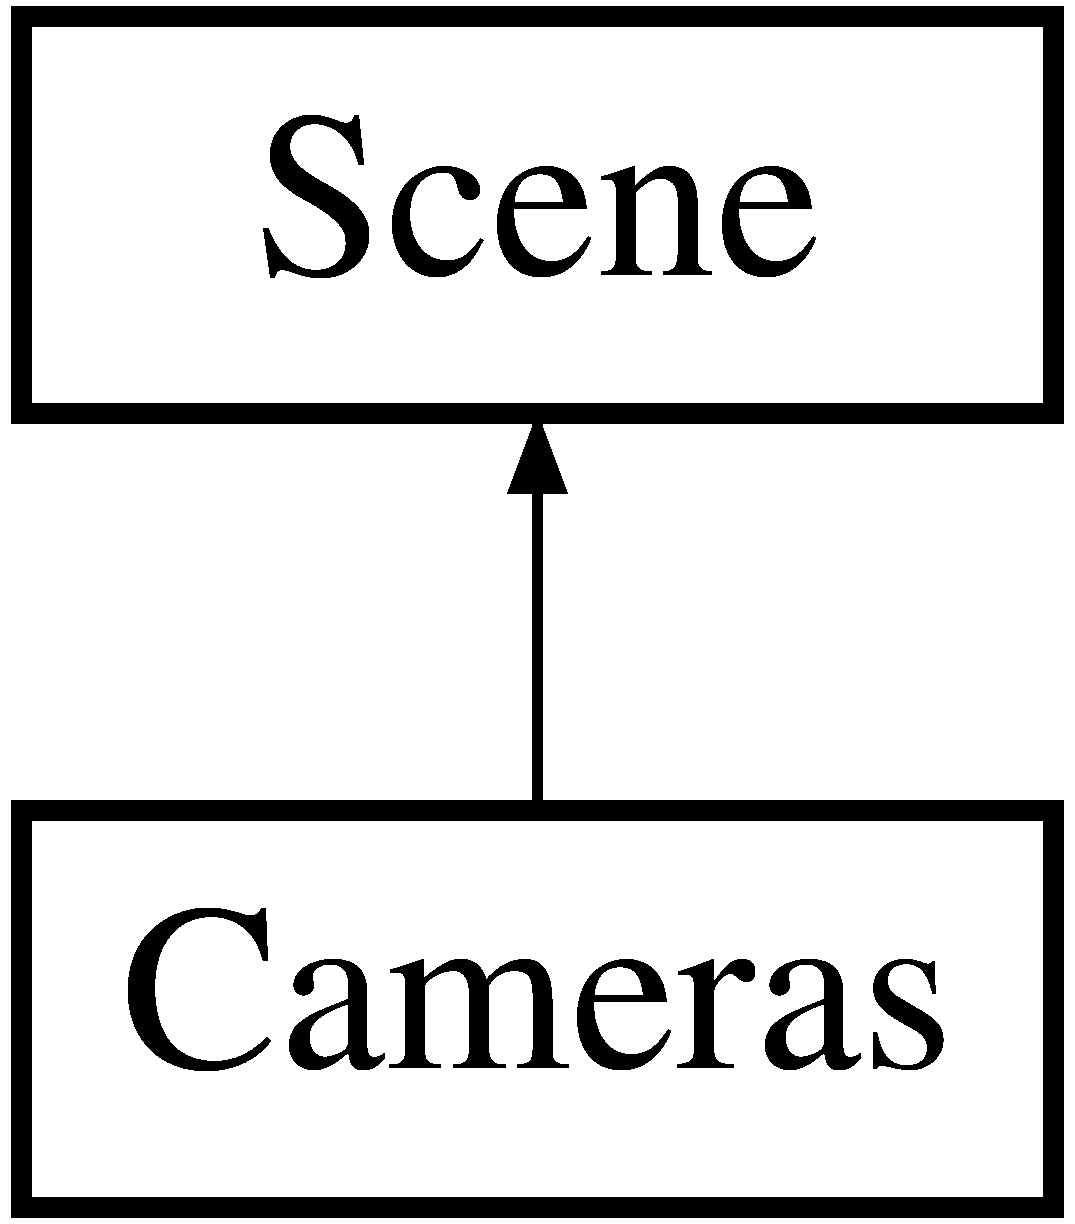
\includegraphics[height=2.000000cm]{class_cameras}
\end{center}
\end{figure}
\subsection*{Public Member Functions}
\begin{DoxyCompactItemize}
\item 
\hyperlink{class_cameras_a14342354c24f588c24e004a722849c3d}{Cameras} (void)
\begin{DoxyCompactList}\small\item\em Default constructor. \end{DoxyCompactList}\item 
\hyperlink{class_cameras_a7de763b562cce2a06cb120610987cd29}{$\sim$\-Cameras} (void)
\begin{DoxyCompactList}\small\item\em Default destructor. \end{DoxyCompactList}\item 
\hyperlink{class_camera}{Camera} $\ast$ \hyperlink{class_cameras_a436b481bf293ec6dfa09d2f89054c54b}{add\-Camera} (const std\-::string \&name)
\begin{DoxyCompactList}\small\item\em add\-Camera takes a name for a camera and returns a handle to a newly created camera. \end{DoxyCompactList}\item 
void \hyperlink{class_cameras_a9dee7bf1f2c56176c461fa2617ce4549}{pop\-Camera} (void)
\begin{DoxyCompactList}\small\item\em pop\-Camera removes the most recently added \hyperlink{class_camera}{Camera} from the scene. \end{DoxyCompactList}\item 
\hyperlink{class_camera}{Camera} $\ast$ \hyperlink{class_cameras_a971e1ffd27ff38d58f83996f87700e82}{next} (void)
\begin{DoxyCompactList}\small\item\em Sets the active camera to the next available one in the collection. \end{DoxyCompactList}\item 
\hyperlink{class_camera}{Camera} $\ast$ \hyperlink{class_cameras_a90eb5a3dda940ed494f592d094580dd8}{prev} (void)
\begin{DoxyCompactList}\small\item\em Sets the active \hyperlink{class_camera}{Camera} to the previous available one in the collection. \end{DoxyCompactList}\item 
\hyperlink{class_camera}{Camera} $\ast$ \hyperlink{class_cameras_a6002cbceb6a93092a1a029af486349a0}{active} (void) const 
\begin{DoxyCompactList}\small\item\em active returns the \hyperlink{class_camera}{Camera} in the collection that is considered 'active'. \end{DoxyCompactList}\item 
size\-\_\-t \hyperlink{class_cameras_acf7e92b5163efeeb88543e605d436a0e}{num\-Cameras} (void) const 
\begin{DoxyCompactList}\small\item\em num\-Cameras fetches the number of \hyperlink{class_cameras}{Cameras} in the collection. \end{DoxyCompactList}\item 
void \hyperlink{class_cameras_ac4fee80c5cd473ee4fa2360a95857da7}{idle\-Motion} (void)
\begin{DoxyCompactList}\small\item\em idle\-Motion calls the idle method on all child cameras. \end{DoxyCompactList}\item 
void \hyperlink{class_cameras_a0d0b08d599d471c0070665006f3bc437}{resize} (int width, int height)
\begin{DoxyCompactList}\small\item\em resize informs the \hyperlink{class_cameras}{Cameras} collection of the new window size. \end{DoxyCompactList}\item 
void \hyperlink{class_cameras_a9d3b24eec1504127e4942aa0e9412ae7}{calculate\-Viewports} (void)
\begin{DoxyCompactList}\small\item\em For each \hyperlink{class_camera}{Camera} in the collection, computes the position and size of that \hyperlink{class_camera}{Camera}'s viewport in a split-\/screen, single-\/window configuration. \end{DoxyCompactList}\item 
void \hyperlink{class_cameras_adeb29c1d639fcfbae4c68017bc8ef4d4}{view} (void($\ast$draw\-\_\-func)(void))
\begin{DoxyCompactList}\small\item\em view calls the view method on all child cameras, followed by the provided draw function. \end{DoxyCompactList}\item 
\hyperlink{class_camera}{Camera} $\ast$ \hyperlink{class_cameras_a8a6c7958396c6b0d07380aa762b15fcc}{obj2\-Cam} (std\-::list$<$ \hyperlink{class_object}{Object} $\ast$ $>$\-::iterator \&it)
\begin{DoxyCompactList}\small\item\em obj2\-Cam is a gross hack; the function is used as a utility to convert \hyperlink{class_object}{Object} pointers to \hyperlink{class_camera}{Camera} pointers safely. \end{DoxyCompactList}\item 
virtual void \hyperlink{class_scene_a7137a7302c21ac4dd44e746bfb6f7cf8}{Shader} (G\-Luint g\-Shader)
\begin{DoxyCompactList}\small\item\em Sets the Default shader for the scene. \end{DoxyCompactList}\item 
G\-Luint \hyperlink{class_scene_af1e8ba8802f3bf83cebbfcbf3ed7c333}{Shader} (void)
\begin{DoxyCompactList}\small\item\em Retrieves the handle for the default shader for the scene. \end{DoxyCompactList}\item 
\hypertarget{class_scene_a366b5dec1ecf66a887b4d0dedcd1aa3b}{\hyperlink{class_object}{Object} $\ast$ {\bfseries Add\-Object} (const std\-::string \&obj\-Name, G\-Luint Object\-\_\-\-Shader=0)}\label{class_scene_a366b5dec1ecf66a887b4d0dedcd1aa3b}

\item 
\hypertarget{class_scene_a3bd9fa1058f506c04162b9283e97d20e}{void {\bfseries Del\-Object} (const std\-::string \&obj\-Name)}\label{class_scene_a3bd9fa1058f506c04162b9283e97d20e}

\item 
\hypertarget{class_scene_a43fd3c56db5dc940d1724b9573c9a360}{void {\bfseries Del\-Object} (void)}\label{class_scene_a43fd3c56db5dc940d1724b9573c9a360}

\item 
\hypertarget{class_scene_abdfd15e7987aa261840d5ecc265170df}{void {\bfseries Pop\-Object} (void)}\label{class_scene_abdfd15e7987aa261840d5ecc265170df}

\item 
\hypertarget{class_scene_a82759ded1f6f87a91b8d10ed87501958}{void \hyperlink{class_scene_a82759ded1f6f87a91b8d10ed87501958}{Destroy\-Object} (void)}\label{class_scene_a82759ded1f6f87a91b8d10ed87501958}

\begin{DoxyCompactList}\small\item\em Completely remove this object and all his children. \end{DoxyCompactList}\item 
\hypertarget{class_scene_ad5a91c929b569b9111061eec16b3febf}{void {\bfseries Draw} (void)}\label{class_scene_ad5a91c929b569b9111061eec16b3febf}

\item 
\hypertarget{class_scene_ae9b69d8db8a46991017635f22e45baad}{\hyperlink{class_object}{Object} $\ast$ {\bfseries operator\mbox{[}$\,$\mbox{]}} (const std\-::string \&objname)}\label{class_scene_ae9b69d8db8a46991017635f22e45baad}

\end{DoxyCompactItemize}
\subsection*{Protected Member Functions}
\begin{DoxyCompactItemize}
\item 
void \hyperlink{class_scene_a8bbe0e5b1bfc71034b18e240e86aa285}{Delete\-Object} (\hyperlink{class_object}{Object} $\ast$obj)
\begin{DoxyCompactList}\small\item\em Delete\-Object is the actual implementation function that will remove an \hyperlink{class_object}{Object} from the \hyperlink{class_scene}{Scene} list and \hyperlink{class_scene}{Scene} map, then free the object. \end{DoxyCompactList}\item 
\hypertarget{class_scene_ae8d51ddc196248a7cbd1f3640851dbd4}{void {\bfseries Insert\-Object} (const std\-::string name, \hyperlink{class_object}{Object} $\ast$obj)}\label{class_scene_ae8d51ddc196248a7cbd1f3640851dbd4}

\end{DoxyCompactItemize}
\subsection*{Protected Attributes}
\begin{DoxyCompactItemize}
\item 
\hypertarget{class_scene_acdd0123ca6b2d64d8d447bb485b235fc}{std\-::list$<$ \hyperlink{class_object}{Object} $\ast$ $>$ {\bfseries \-\_\-list}}\label{class_scene_acdd0123ca6b2d64d8d447bb485b235fc}

\item 
\hypertarget{class_scene_a8bd5d86484a12255b26b92b6cbf8d29a}{std\-::map$<$ std\-::string, \hyperlink{class_object}{Object} $\ast$ $>$ {\bfseries \-\_\-map}}\label{class_scene_a8bd5d86484a12255b26b92b6cbf8d29a}

\item 
\hypertarget{class_scene_ae87ca5350fcc595f3f15a4fd3c39f3d9}{std\-::list$<$ \hyperlink{class_object}{Object} $\ast$ $>$\-::iterator {\bfseries \-\_\-current\-Obj}}\label{class_scene_ae87ca5350fcc595f3f15a4fd3c39f3d9}

\item 
\hypertarget{class_scene_a8f9bdd8ec5edb1f414fbd314a36e2724}{G\-Luint {\bfseries \-\_\-g\-Shader}}\label{class_scene_a8f9bdd8ec5edb1f414fbd314a36e2724}

\end{DoxyCompactItemize}
\subsection*{Private Attributes}
\begin{DoxyCompactItemize}
\item 
\hypertarget{class_cameras_a2c40cd131741e1904fdfb024006258fd}{\hyperlink{struct_angel_1_1vec2}{Angel\-::vec2} \hyperlink{class_cameras_a2c40cd131741e1904fdfb024006258fd}{\-\_\-size}}\label{class_cameras_a2c40cd131741e1904fdfb024006258fd}

\begin{DoxyCompactList}\small\item\em \-\_\-size is a simple vec2 (x,y) that contains the size of the screen. \end{DoxyCompactList}\end{DoxyCompactItemize}


\subsection{Detailed Description}
The \hyperlink{class_cameras}{Cameras} class represents a group of logical cameras for a model view. Each camera possesses its own current viewing angle, and an absolute position in space. 

\begin{DoxyAuthor}{Author}
John Huston, \href{mailto:jhuston@cs.uml.edu}{\tt jhuston@cs.\-uml.\-edu} 
\end{DoxyAuthor}
\begin{DoxySince}{Since}
28 Nov 2012
\end{DoxySince}
Each \hyperlink{class_camera}{Camera} possesses its own C\-T\-M which can be resent to the G\-P\-U at will. 

Definition at line 29 of file Cameras.\-hpp.



\subsection{Constructor \& Destructor Documentation}
\hypertarget{class_cameras_a14342354c24f588c24e004a722849c3d}{\index{Cameras@{Cameras}!Cameras@{Cameras}}
\index{Cameras@{Cameras}!Cameras@{Cameras}}
\subsubsection[{Cameras}]{\setlength{\rightskip}{0pt plus 5cm}Cameras\-::\-Cameras (
\begin{DoxyParamCaption}
\item[{void}]{}
\end{DoxyParamCaption}
)}}\label{class_cameras_a14342354c24f588c24e004a722849c3d}


Default constructor. 

Nothing special. 

Definition at line 19 of file Cameras.\-cpp.

\hypertarget{class_cameras_a7de763b562cce2a06cb120610987cd29}{\index{Cameras@{Cameras}!$\sim$\-Cameras@{$\sim$\-Cameras}}
\index{$\sim$\-Cameras@{$\sim$\-Cameras}!Cameras@{Cameras}}
\subsubsection[{$\sim$\-Cameras}]{\setlength{\rightskip}{0pt plus 5cm}Cameras\-::$\sim$\-Cameras (
\begin{DoxyParamCaption}
\item[{void}]{}
\end{DoxyParamCaption}
)}}\label{class_cameras_a7de763b562cce2a06cb120610987cd29}


Default destructor. 

Nothing special here, either. 

Definition at line 26 of file Cameras.\-cpp.



\subsection{Member Function Documentation}
\hypertarget{class_cameras_a6002cbceb6a93092a1a029af486349a0}{\index{Cameras@{Cameras}!active@{active}}
\index{active@{active}!Cameras@{Cameras}}
\subsubsection[{active}]{\setlength{\rightskip}{0pt plus 5cm}{\bf Camera} $\ast$ Cameras\-::active (
\begin{DoxyParamCaption}
\item[{void}]{}
\end{DoxyParamCaption}
) const}}\label{class_cameras_a6002cbceb6a93092a1a029af486349a0}


active returns the \hyperlink{class_camera}{Camera} in the collection that is considered 'active'. 

\begin{DoxyReturn}{Returns}
A pointer to the currently selected, active \hyperlink{class_camera}{Camera}. 
\end{DoxyReturn}


Definition at line 86 of file Cameras.\-cpp.

\hypertarget{class_cameras_a436b481bf293ec6dfa09d2f89054c54b}{\index{Cameras@{Cameras}!add\-Camera@{add\-Camera}}
\index{add\-Camera@{add\-Camera}!Cameras@{Cameras}}
\subsubsection[{add\-Camera}]{\setlength{\rightskip}{0pt plus 5cm}{\bf Camera} $\ast$ Cameras\-::add\-Camera (
\begin{DoxyParamCaption}
\item[{const std\-::string \&}]{name}
\end{DoxyParamCaption}
)}}\label{class_cameras_a436b481bf293ec6dfa09d2f89054c54b}


add\-Camera takes a name for a camera and returns a handle to a newly created camera. 


\begin{DoxyParams}{Parameters}
{\em name} & The name of the new camera to create. \\
\hline
\end{DoxyParams}
\begin{DoxyReturn}{Returns}
A Pointer to a newly created \hyperlink{class_camera}{Camera} object. 
\end{DoxyReturn}


Definition at line 35 of file Cameras.\-cpp.

\hypertarget{class_cameras_a9d3b24eec1504127e4942aa0e9412ae7}{\index{Cameras@{Cameras}!calculate\-Viewports@{calculate\-Viewports}}
\index{calculate\-Viewports@{calculate\-Viewports}!Cameras@{Cameras}}
\subsubsection[{calculate\-Viewports}]{\setlength{\rightskip}{0pt plus 5cm}void Cameras\-::calculate\-Viewports (
\begin{DoxyParamCaption}
\item[{void}]{}
\end{DoxyParamCaption}
)}}\label{class_cameras_a9d3b24eec1504127e4942aa0e9412ae7}


For each \hyperlink{class_camera}{Camera} in the collection, computes the position and size of that \hyperlink{class_camera}{Camera}'s viewport in a split-\/screen, single-\/window configuration. 

The \hyperlink{class_camera}{Camera} object is updated with the new information.

\begin{DoxyReturn}{Returns}
void.

void. 
\end{DoxyReturn}


Definition at line 141 of file Cameras.\-cpp.

\hypertarget{class_scene_a8bbe0e5b1bfc71034b18e240e86aa285}{\index{Cameras@{Cameras}!Delete\-Object@{Delete\-Object}}
\index{Delete\-Object@{Delete\-Object}!Cameras@{Cameras}}
\subsubsection[{Delete\-Object}]{\setlength{\rightskip}{0pt plus 5cm}void Scene\-::\-Delete\-Object (
\begin{DoxyParamCaption}
\item[{{\bf Object} $\ast$}]{obj}
\end{DoxyParamCaption}
)\hspace{0.3cm}{\ttfamily [protected]}, {\ttfamily [inherited]}}}\label{class_scene_a8bbe0e5b1bfc71034b18e240e86aa285}


Delete\-Object is the actual implementation function that will remove an \hyperlink{class_object}{Object} from the \hyperlink{class_scene}{Scene} list and \hyperlink{class_scene}{Scene} map, then free the object. 


\begin{DoxyParams}{Parameters}
{\em obj} & The pointer to the object to free. \\
\hline
\end{DoxyParams}


Definition at line 76 of file Scene.\-cpp.

\hypertarget{class_cameras_ac4fee80c5cd473ee4fa2360a95857da7}{\index{Cameras@{Cameras}!idle\-Motion@{idle\-Motion}}
\index{idle\-Motion@{idle\-Motion}!Cameras@{Cameras}}
\subsubsection[{idle\-Motion}]{\setlength{\rightskip}{0pt plus 5cm}void Cameras\-::idle\-Motion (
\begin{DoxyParamCaption}
\item[{void}]{}
\end{DoxyParamCaption}
)}}\label{class_cameras_ac4fee80c5cd473ee4fa2360a95857da7}


idle\-Motion calls the idle method on all child cameras. 

Intended to be called during the \hyperlink{ds_8cpp_a01131b63acf241e9db91704d89ce15d2}{idle()} loop in G\-L\-U\-T.

\begin{DoxyReturn}{Returns}
void. 
\end{DoxyReturn}


Definition at line 111 of file Cameras.\-cpp.

\hypertarget{class_cameras_a971e1ffd27ff38d58f83996f87700e82}{\index{Cameras@{Cameras}!next@{next}}
\index{next@{next}!Cameras@{Cameras}}
\subsubsection[{next}]{\setlength{\rightskip}{0pt plus 5cm}{\bf Camera} $\ast$ Cameras\-::next (
\begin{DoxyParamCaption}
\item[{void}]{}
\end{DoxyParamCaption}
)}}\label{class_cameras_a971e1ffd27ff38d58f83996f87700e82}


Sets the active camera to the next available one in the collection. 

Sets the active \hyperlink{class_camera}{Camera} to the next available one in the collection.

\begin{DoxyReturn}{Returns}
A pointer to the newly active \hyperlink{class_camera}{Camera}. 
\end{DoxyReturn}


Definition at line 64 of file Cameras.\-cpp.

\hypertarget{class_cameras_acf7e92b5163efeeb88543e605d436a0e}{\index{Cameras@{Cameras}!num\-Cameras@{num\-Cameras}}
\index{num\-Cameras@{num\-Cameras}!Cameras@{Cameras}}
\subsubsection[{num\-Cameras}]{\setlength{\rightskip}{0pt plus 5cm}size\-\_\-t Cameras\-::num\-Cameras (
\begin{DoxyParamCaption}
\item[{void}]{}
\end{DoxyParamCaption}
) const}}\label{class_cameras_acf7e92b5163efeeb88543e605d436a0e}


num\-Cameras fetches the number of \hyperlink{class_cameras}{Cameras} in the collection. 

\begin{DoxyReturn}{Returns}
an unsigned integer, the number of \hyperlink{class_cameras}{Cameras} in the collection. 
\end{DoxyReturn}


Definition at line 101 of file Cameras.\-cpp.

\hypertarget{class_cameras_a8a6c7958396c6b0d07380aa762b15fcc}{\index{Cameras@{Cameras}!obj2\-Cam@{obj2\-Cam}}
\index{obj2\-Cam@{obj2\-Cam}!Cameras@{Cameras}}
\subsubsection[{obj2\-Cam}]{\setlength{\rightskip}{0pt plus 5cm}{\bf Camera} $\ast$ Cameras\-::obj2\-Cam (
\begin{DoxyParamCaption}
\item[{std\-::list$<$ {\bf Object} $\ast$ $>$\-::iterator \&}]{it}
\end{DoxyParamCaption}
)}}\label{class_cameras_a8a6c7958396c6b0d07380aa762b15fcc}


obj2\-Cam is a gross hack; the function is used as a utility to convert \hyperlink{class_object}{Object} pointers to \hyperlink{class_camera}{Camera} pointers safely. 

F\-I\-X\-M\-E\-: Refactor the inheritance here to make this less hacky.


\begin{DoxyParams}{Parameters}
{\em it} & A list$<$\-Object$\ast$$>$ iterator that points to the \hyperlink{class_object}{Object}.\\
\hline
\end{DoxyParams}
\begin{DoxyReturn}{Returns}
A pointer to a \hyperlink{class_camera}{Camera} object. 
\end{DoxyReturn}


Definition at line 249 of file Cameras.\-cpp.

\hypertarget{class_cameras_a9dee7bf1f2c56176c461fa2617ce4549}{\index{Cameras@{Cameras}!pop\-Camera@{pop\-Camera}}
\index{pop\-Camera@{pop\-Camera}!Cameras@{Cameras}}
\subsubsection[{pop\-Camera}]{\setlength{\rightskip}{0pt plus 5cm}void Cameras\-::pop\-Camera (
\begin{DoxyParamCaption}
\item[{void}]{}
\end{DoxyParamCaption}
)}}\label{class_cameras_a9dee7bf1f2c56176c461fa2617ce4549}


pop\-Camera removes the most recently added \hyperlink{class_camera}{Camera} from the scene. 

\begin{DoxyReturn}{Returns}
void. 
\end{DoxyReturn}


Definition at line 50 of file Cameras.\-cpp.

\hypertarget{class_cameras_a90eb5a3dda940ed494f592d094580dd8}{\index{Cameras@{Cameras}!prev@{prev}}
\index{prev@{prev}!Cameras@{Cameras}}
\subsubsection[{prev}]{\setlength{\rightskip}{0pt plus 5cm}{\bf Camera} $\ast$ Cameras\-::prev (
\begin{DoxyParamCaption}
\item[{void}]{}
\end{DoxyParamCaption}
)}}\label{class_cameras_a90eb5a3dda940ed494f592d094580dd8}


Sets the active \hyperlink{class_camera}{Camera} to the previous available one in the collection. 

\begin{DoxyReturn}{Returns}
A pointer to the newly active \hyperlink{class_camera}{Camera}. 
\end{DoxyReturn}


Definition at line 75 of file Cameras.\-cpp.

\hypertarget{class_cameras_a0d0b08d599d471c0070665006f3bc437}{\index{Cameras@{Cameras}!resize@{resize}}
\index{resize@{resize}!Cameras@{Cameras}}
\subsubsection[{resize}]{\setlength{\rightskip}{0pt plus 5cm}void Cameras\-::resize (
\begin{DoxyParamCaption}
\item[{int}]{width, }
\item[{int}]{height}
\end{DoxyParamCaption}
)}}\label{class_cameras_a0d0b08d599d471c0070665006f3bc437}


resize informs the \hyperlink{class_cameras}{Cameras} collection of the new window size. 

Intended to be called from the G\-L\-U\-T main loop. This method also invokes \hyperlink{class_cameras_a9d3b24eec1504127e4942aa0e9412ae7}{Cameras\-::calculate\-Viewports}.


\begin{DoxyParams}{Parameters}
{\em width} & The new window width. \\
\hline
{\em height} & The new window height.\\
\hline
\end{DoxyParams}
\begin{DoxyReturn}{Returns}
void. 
\end{DoxyReturn}


Definition at line 128 of file Cameras.\-cpp.

\hypertarget{class_scene_a7137a7302c21ac4dd44e746bfb6f7cf8}{\index{Cameras@{Cameras}!Shader@{Shader}}
\index{Shader@{Shader}!Cameras@{Cameras}}
\subsubsection[{Shader}]{\setlength{\rightskip}{0pt plus 5cm}void Scene\-::\-Shader (
\begin{DoxyParamCaption}
\item[{G\-Luint}]{g\-Shader}
\end{DoxyParamCaption}
)\hspace{0.3cm}{\ttfamily [virtual]}, {\ttfamily [inherited]}}}\label{class_scene_a7137a7302c21ac4dd44e746bfb6f7cf8}


Sets the Default shader for the scene. 

In the context of inheritance by objects, This sets the shader to use to render the physical object.


\begin{DoxyParams}{Parameters}
{\em g\-Shader} & The G\-Luint handle to the shader to use.\\
\hline
\end{DoxyParams}
\begin{DoxyReturn}{Returns}
void. 
\end{DoxyReturn}


Reimplemented in \hyperlink{class_object_aa52c30bca96800cecba55f446e147859}{Object}.



Definition at line 54 of file Scene.\-cpp.

\hypertarget{class_scene_af1e8ba8802f3bf83cebbfcbf3ed7c333}{\index{Cameras@{Cameras}!Shader@{Shader}}
\index{Shader@{Shader}!Cameras@{Cameras}}
\subsubsection[{Shader}]{\setlength{\rightskip}{0pt plus 5cm}G\-Luint Scene\-::\-Shader (
\begin{DoxyParamCaption}
\item[{void}]{}
\end{DoxyParamCaption}
)\hspace{0.3cm}{\ttfamily [inherited]}}}\label{class_scene_af1e8ba8802f3bf83cebbfcbf3ed7c333}


Retrieves the handle for the default shader for the scene. 

In the context of inheritance by objects, This retrieves the shader handle to use to draw the object.

\begin{DoxyReturn}{Returns}
A G\-Luint handle to the shader program. 
\end{DoxyReturn}


Definition at line 66 of file Scene.\-cpp.

\hypertarget{class_cameras_adeb29c1d639fcfbae4c68017bc8ef4d4}{\index{Cameras@{Cameras}!view@{view}}
\index{view@{view}!Cameras@{Cameras}}
\subsubsection[{view}]{\setlength{\rightskip}{0pt plus 5cm}void Cameras\-::view (
\begin{DoxyParamCaption}
\item[{void($\ast$)(void)}]{draw\-\_\-func}
\end{DoxyParamCaption}
)}}\label{class_cameras_adeb29c1d639fcfbae4c68017bc8ef4d4}


view calls the view method on all child cameras, followed by the provided draw function. 

Intended to be called during the \hyperlink{ds_8cpp_a4ea013001a5fb47853d0fab8f8de35cd}{display()} portion of the G\-L\-U\-T main loop.

\hyperlink{class_cameras_adeb29c1d639fcfbae4c68017bc8ef4d4}{view()} is intended to \char`\"{}set up\char`\"{} the object, but not actually draw it.


\begin{DoxyParams}{Parameters}
{\em draw\-\_\-func} & A pointer to a function that will actually draw the object. \\
\hline
\end{DoxyParams}


Definition at line 232 of file Cameras.\-cpp.



The documentation for this class was generated from the following files\-:\begin{DoxyCompactItemize}
\item 
\hyperlink{_cameras_8hpp}{Cameras.\-hpp}\item 
\hyperlink{_cameras_8cpp}{Cameras.\-cpp}\end{DoxyCompactItemize}

\hypertarget{class_engine}{\section{Engine Class Reference}
\label{class_engine}\index{Engine@{Engine}}
}


The \hyperlink{class_engine}{Engine} class is a singleton-\/style class which helps keep track of instances of important objects (for \hyperlink{class_cameras}{Cameras}, Objects, etc) as well as some settings and variables that would otherwise clog up global namespace.  




{\ttfamily \#include $<$Engine.\-hpp$>$}

\subsection*{Public Member Functions}
\begin{DoxyCompactItemize}
\item 
\hyperlink{class_cameras}{Cameras} $\ast$ \hyperlink{class_engine_a2b2c1cd59c9a5c903bf466284012ce4c}{cams} (void)
\begin{DoxyCompactList}\small\item\em Retrieves a pointer to the \hyperlink{class_camera}{Camera} List. \end{DoxyCompactList}\item 
\hyperlink{class_scene}{Scene} $\ast$ \hyperlink{class_engine_a782cf288c161986d0ac0eb48cd187c4d}{root\-Scene} (void)
\begin{DoxyCompactList}\small\item\em Retrieves a pointer to the Root, top-\/level \hyperlink{class_scene}{Scene} graph. \end{DoxyCompactList}\item 
\hyperlink{class_screen}{Screen} $\ast$ \hyperlink{class_engine_ad4429218b5aed162269094c6571a2520}{main\-Screen} (void)
\begin{DoxyCompactList}\small\item\em Retrieves a pointer to the core '\hyperlink{class_screen}{Screen}' object. \end{DoxyCompactList}\item 
bool \hyperlink{class_engine_ae3658976c5ab1f0c912d2c7d5747cb67}{opt} (const std\-::string \&Option)
\begin{DoxyCompactList}\small\item\em opt retrieves the current setting of an option in the \hyperlink{class_engine}{Engine}. \end{DoxyCompactList}\item 
void \hyperlink{class_engine_a797b0b934a94cd2ea7ab1c11083e425c}{opt} (const std\-::string \&Option, bool setting)
\begin{DoxyCompactList}\small\item\em opt, with a second parameter, sets an \hyperlink{class_engine}{Engine} option. \end{DoxyCompactList}\item 
bool \hyperlink{class_engine_a81f16979bc330c46675e4d7ffab5eff9}{set} (const std\-::string \&Option)
\begin{DoxyCompactList}\small\item\em set checks to see if an option has been explicitly set to either True/\-False. \end{DoxyCompactList}\item 
bool \hyperlink{class_engine_a0e6265ae2700bda2f21abd308430637a}{flip} (const std\-::string \&Option)
\begin{DoxyCompactList}\small\item\em flip changes a setting from its current value to its negated form. \end{DoxyCompactList}\item 
\hypertarget{class_engine_a4850643b0f929d8021115cf37d7ab608}{\hyperlink{class_engine_a4850643b0f929d8021115cf37d7ab608}{$\sim$\-Engine} (void)}\label{class_engine_a4850643b0f929d8021115cf37d7ab608}

\begin{DoxyCompactList}\small\item\em Default, non-\/virtual destructor. \end{DoxyCompactList}\end{DoxyCompactItemize}
\subsection*{Static Public Member Functions}
\begin{DoxyCompactItemize}
\item 
static \hyperlink{class_engine}{Engine} $\ast$ \hyperlink{class_engine_a6cbf9ec80a4a3bb245355ff70498dba0}{instance} (void)
\begin{DoxyCompactList}\small\item\em instance returns, or creates and then returns, a pointer to the \hyperlink{class_engine}{Engine} object. \end{DoxyCompactList}\end{DoxyCompactItemize}
\subsection*{Private Member Functions}
\begin{DoxyCompactItemize}
\item 
\hyperlink{class_engine_a9ad87e382195a05d5d310a2fb3e357fd}{Engine} (void)
\begin{DoxyCompactList}\small\item\em Default constructor. \end{DoxyCompactList}\item 
\hyperlink{class_engine_a8e027119a62020acddedd0a14fb44033}{Engine} (const \hyperlink{class_engine}{Engine} \&copy)
\begin{DoxyCompactList}\small\item\em Copy constructor. \end{DoxyCompactList}\item 
\hyperlink{class_engine}{Engine} \& \hyperlink{class_engine_a09761dabaae6f48bd5c612acea76a9bf}{operator=} (\hyperlink{class_engine}{Engine} \&assign)
\begin{DoxyCompactList}\small\item\em Assignment operator. \end{DoxyCompactList}\end{DoxyCompactItemize}
\subsection*{Private Attributes}
\begin{DoxyCompactItemize}
\item 
\hypertarget{class_engine_afc244649d4b31f59f2ef91754472b281}{\hyperlink{class_scene}{Scene} \hyperlink{class_engine_afc244649d4b31f59f2ef91754472b281}{\-\_\-scene}}\label{class_engine_afc244649d4b31f59f2ef91754472b281}

\begin{DoxyCompactList}\small\item\em The root \hyperlink{class_scene}{Scene} graph for the \hyperlink{class_engine}{Engine}. \end{DoxyCompactList}\item 
\hypertarget{class_engine_a181e11b6fd26698bc173647ab2471c8c}{\hyperlink{class_screen}{Screen} \hyperlink{class_engine_a181e11b6fd26698bc173647ab2471c8c}{\-\_\-screen}}\label{class_engine_a181e11b6fd26698bc173647ab2471c8c}

\begin{DoxyCompactList}\small\item\em The core \char`\"{}\-Screen\char`\"{} object for the \hyperlink{class_engine}{Engine}. \end{DoxyCompactList}\item 
\hypertarget{class_engine_a467d917952b89ef23f7a045e4f87218a}{\hyperlink{_engine_8hpp_a35f3ec1606bb0642e48d2e62fea0d6a6}{Settings\-Map} \hyperlink{class_engine_a467d917952b89ef23f7a045e4f87218a}{\-\_\-engine\-Settings}}\label{class_engine_a467d917952b89ef23f7a045e4f87218a}

\begin{DoxyCompactList}\small\item\em \-\_\-engine\-Settings is a std\-::map that contains a series of $<$std\-::string, bool$>$ pairs that represent our \hyperlink{class_engine}{Engine} options. \end{DoxyCompactList}\end{DoxyCompactItemize}
\subsection*{Static Private Attributes}
\begin{DoxyCompactItemize}
\item 
\hypertarget{class_engine_ae494a590056c4594f1f3cb39e4d18994}{static \hyperlink{class_engine}{Engine} $\ast$ \hyperlink{class_engine_ae494a590056c4594f1f3cb39e4d18994}{\-\_\-engine\-Singleton} = N\-U\-L\-L}\label{class_engine_ae494a590056c4594f1f3cb39e4d18994}

\begin{DoxyCompactList}\small\item\em static, stateful variable that is our singleton pointer. \end{DoxyCompactList}\end{DoxyCompactItemize}


\subsection{Detailed Description}
The \hyperlink{class_engine}{Engine} class is a singleton-\/style class which helps keep track of instances of important objects (for \hyperlink{class_cameras}{Cameras}, Objects, etc) as well as some settings and variables that would otherwise clog up global namespace. 

\begin{DoxyAuthor}{Author}
John Huston, \href{mailto:jhuston@cs.uml.edu}{\tt jhuston@cs.\-uml.\-edu} 
\end{DoxyAuthor}
\begin{DoxyDate}{Date}
2013-\/03-\/13 
\end{DoxyDate}


Definition at line 32 of file Engine.\-hpp.



\subsection{Constructor \& Destructor Documentation}
\hypertarget{class_engine_a9ad87e382195a05d5d310a2fb3e357fd}{\index{Engine@{Engine}!Engine@{Engine}}
\index{Engine@{Engine}!Engine@{Engine}}
\subsubsection[{Engine}]{\setlength{\rightskip}{0pt plus 5cm}Engine\-::\-Engine (
\begin{DoxyParamCaption}
\item[{void}]{}
\end{DoxyParamCaption}
)\hspace{0.3cm}{\ttfamily [private]}}}\label{class_engine_a9ad87e382195a05d5d310a2fb3e357fd}


Default constructor. 

Cannot be called, this is a singleton class. 

Definition at line 40 of file Engine.\-cpp.

\hypertarget{class_engine_a8e027119a62020acddedd0a14fb44033}{\index{Engine@{Engine}!Engine@{Engine}}
\index{Engine@{Engine}!Engine@{Engine}}
\subsubsection[{Engine}]{\setlength{\rightskip}{0pt plus 5cm}Engine\-::\-Engine (
\begin{DoxyParamCaption}
\item[{const {\bf Engine} \&}]{copy}
\end{DoxyParamCaption}
)\hspace{0.3cm}{\ttfamily [private]}}}\label{class_engine_a8e027119a62020acddedd0a14fb44033}


Copy constructor. 

Cannot be called. 
\begin{DoxyParams}{Parameters}
{\em copy} & Not used. \\
\hline
\end{DoxyParams}
\begin{DoxyReturn}{Returns}
Will always throw an exception. 
\end{DoxyReturn}

\begin{DoxyExceptions}{Exceptions}
{\em Will} & always throw std\-::logic\-\_\-error. \\
\hline
\end{DoxyExceptions}


Definition at line 57 of file Engine.\-cpp.



\subsection{Member Function Documentation}
\hypertarget{class_engine_a2b2c1cd59c9a5c903bf466284012ce4c}{\index{Engine@{Engine}!cams@{cams}}
\index{cams@{cams}!Engine@{Engine}}
\subsubsection[{cams}]{\setlength{\rightskip}{0pt plus 5cm}{\bf Cameras} $\ast$ Engine\-::cams (
\begin{DoxyParamCaption}
\item[{void}]{}
\end{DoxyParamCaption}
)}}\label{class_engine_a2b2c1cd59c9a5c903bf466284012ce4c}


Retrieves a pointer to the \hyperlink{class_camera}{Camera} List. 

\begin{DoxyReturn}{Returns}
A pointer to the \hyperlink{class_camera}{Camera} List. 
\end{DoxyReturn}


Definition at line 76 of file Engine.\-cpp.

\hypertarget{class_engine_a0e6265ae2700bda2f21abd308430637a}{\index{Engine@{Engine}!flip@{flip}}
\index{flip@{flip}!Engine@{Engine}}
\subsubsection[{flip}]{\setlength{\rightskip}{0pt plus 5cm}bool Engine\-::flip (
\begin{DoxyParamCaption}
\item[{const std\-::string \&}]{Option}
\end{DoxyParamCaption}
)}}\label{class_engine_a0e6265ae2700bda2f21abd308430637a}


flip changes a setting from its current value to its negated form. 


\begin{DoxyParams}{Parameters}
{\em Option} & The option to toggle. \\
\hline
\end{DoxyParams}
\begin{DoxyReturn}{Returns}
The new, current value of the option. 
\end{DoxyReturn}


Definition at line 139 of file Engine.\-cpp.

\hypertarget{class_engine_a6cbf9ec80a4a3bb245355ff70498dba0}{\index{Engine@{Engine}!instance@{instance}}
\index{instance@{instance}!Engine@{Engine}}
\subsubsection[{instance}]{\setlength{\rightskip}{0pt plus 5cm}{\bf Engine} $\ast$ Engine\-::instance (
\begin{DoxyParamCaption}
\item[{void}]{}
\end{DoxyParamCaption}
)\hspace{0.3cm}{\ttfamily [static]}}}\label{class_engine_a6cbf9ec80a4a3bb245355ff70498dba0}


instance returns, or creates and then returns, a pointer to the \hyperlink{class_engine}{Engine} object. 

All hail the singleton!

\begin{DoxyReturn}{Returns}
A pointer to the \hyperlink{class_engine}{Engine} object. 
\end{DoxyReturn}


Definition at line 29 of file Engine.\-cpp.

\hypertarget{class_engine_ad4429218b5aed162269094c6571a2520}{\index{Engine@{Engine}!main\-Screen@{main\-Screen}}
\index{main\-Screen@{main\-Screen}!Engine@{Engine}}
\subsubsection[{main\-Screen}]{\setlength{\rightskip}{0pt plus 5cm}{\bf Screen} $\ast$ Engine\-::main\-Screen (
\begin{DoxyParamCaption}
\item[{void}]{}
\end{DoxyParamCaption}
)}}\label{class_engine_ad4429218b5aed162269094c6571a2520}


Retrieves a pointer to the core '\hyperlink{class_screen}{Screen}' object. 

\begin{DoxyReturn}{Returns}
A pointer to the core '\hyperlink{class_screen}{Screen}' object. 
\end{DoxyReturn}


Definition at line 96 of file Engine.\-cpp.

\hypertarget{class_engine_a09761dabaae6f48bd5c612acea76a9bf}{\index{Engine@{Engine}!operator=@{operator=}}
\index{operator=@{operator=}!Engine@{Engine}}
\subsubsection[{operator=}]{\setlength{\rightskip}{0pt plus 5cm}{\bf Engine} \& Engine\-::operator= (
\begin{DoxyParamCaption}
\item[{{\bf Engine} \&}]{assign}
\end{DoxyParamCaption}
)\hspace{0.3cm}{\ttfamily [private]}}}\label{class_engine_a09761dabaae6f48bd5c612acea76a9bf}


Assignment operator. 

Cannot be used. This is a singleton class. 
\begin{DoxyParams}{Parameters}
{\em assign} & Not used. \\
\hline
\end{DoxyParams}
\begin{DoxyReturn}{Returns}
Will always throw an exception. 
\end{DoxyReturn}

\begin{DoxyExceptions}{Exceptions}
{\em Will} & always throw std\-::logic\-\_\-error. \\
\hline
\end{DoxyExceptions}


Definition at line 67 of file Engine.\-cpp.

\hypertarget{class_engine_ae3658976c5ab1f0c912d2c7d5747cb67}{\index{Engine@{Engine}!opt@{opt}}
\index{opt@{opt}!Engine@{Engine}}
\subsubsection[{opt}]{\setlength{\rightskip}{0pt plus 5cm}bool Engine\-::opt (
\begin{DoxyParamCaption}
\item[{const std\-::string \&}]{Option}
\end{DoxyParamCaption}
)}}\label{class_engine_ae3658976c5ab1f0c912d2c7d5747cb67}


opt retrieves the current setting of an option in the \hyperlink{class_engine}{Engine}. 


\begin{DoxyParams}{Parameters}
{\em Option} & The name of the option to access. \\
\hline
\end{DoxyParams}
\begin{DoxyReturn}{Returns}
A bool\-: the current value of the setting. 
\end{DoxyReturn}


Definition at line 107 of file Engine.\-cpp.

\hypertarget{class_engine_a797b0b934a94cd2ea7ab1c11083e425c}{\index{Engine@{Engine}!opt@{opt}}
\index{opt@{opt}!Engine@{Engine}}
\subsubsection[{opt}]{\setlength{\rightskip}{0pt plus 5cm}void Engine\-::opt (
\begin{DoxyParamCaption}
\item[{const std\-::string \&}]{Option, }
\item[{bool}]{setting}
\end{DoxyParamCaption}
)}}\label{class_engine_a797b0b934a94cd2ea7ab1c11083e425c}


opt, with a second parameter, sets an \hyperlink{class_engine}{Engine} option. 


\begin{DoxyParams}{Parameters}
{\em Option} & The name of the option to set. \\
\hline
{\em setting} & The value to give the option. \\
\hline
\end{DoxyParams}
\begin{DoxyReturn}{Returns}
void. 
\end{DoxyReturn}


Definition at line 117 of file Engine.\-cpp.

\hypertarget{class_engine_a782cf288c161986d0ac0eb48cd187c4d}{\index{Engine@{Engine}!root\-Scene@{root\-Scene}}
\index{root\-Scene@{root\-Scene}!Engine@{Engine}}
\subsubsection[{root\-Scene}]{\setlength{\rightskip}{0pt plus 5cm}{\bf Scene} $\ast$ Engine\-::root\-Scene (
\begin{DoxyParamCaption}
\item[{void}]{}
\end{DoxyParamCaption}
)}}\label{class_engine_a782cf288c161986d0ac0eb48cd187c4d}


Retrieves a pointer to the Root, top-\/level \hyperlink{class_scene}{Scene} graph. 

\begin{DoxyReturn}{Returns}
A pointer to the Root-\/level \hyperlink{class_scene}{Scene} graph. 
\end{DoxyReturn}


Definition at line 86 of file Engine.\-cpp.

\hypertarget{class_engine_a81f16979bc330c46675e4d7ffab5eff9}{\index{Engine@{Engine}!set@{set}}
\index{set@{set}!Engine@{Engine}}
\subsubsection[{set}]{\setlength{\rightskip}{0pt plus 5cm}bool Engine\-::set (
\begin{DoxyParamCaption}
\item[{const std\-::string \&}]{Option}
\end{DoxyParamCaption}
)}}\label{class_engine_a81f16979bc330c46675e4d7ffab5eff9}


set checks to see if an option has been explicitly set to either True/\-False. 


\begin{DoxyParams}{Parameters}
{\em Option} & The option to check the existence of \\
\hline
\end{DoxyParams}
\begin{DoxyReturn}{Returns}
A boolean\-: True if the option has been set, False otherwise. 
\end{DoxyReturn}


Definition at line 127 of file Engine.\-cpp.



The documentation for this class was generated from the following files\-:\begin{DoxyCompactItemize}
\item 
\hyperlink{_engine_8hpp}{Engine.\-hpp}\item 
\hyperlink{_engine_8cpp}{Engine.\-cpp}\end{DoxyCompactItemize}

\hypertarget{class_tiem_spelchk_1_1_lurn2_spiel_nub}{\section{Tiem\-Spelchk\-:\-:Lurn2\-Spiel\-Nub Class Reference}
\label{class_tiem_spelchk_1_1_lurn2_spiel_nub}\index{Tiem\-Spelchk\-::\-Lurn2\-Spiel\-Nub@{Tiem\-Spelchk\-::\-Lurn2\-Spiel\-Nub}}
}
\subsection*{Public Member Functions}
\begin{DoxyCompactItemize}
\item 
\hypertarget{class_tiem_spelchk_1_1_lurn2_spiel_nub_a3a84a37ba97831308f639b9e2bf7d9f8}{void {\bfseries set\-Callback} (boost\-::function$<$ void(int, double, double, double)$>$ head\-C\-B)}\label{class_tiem_spelchk_1_1_lurn2_spiel_nub_a3a84a37ba97831308f639b9e2bf7d9f8}

\item 
\hypertarget{class_tiem_spelchk_1_1_lurn2_spiel_nub_a29b93d8ad5bbcefad6df00b4a23f4fc4}{int {\bfseries Start} ()}\label{class_tiem_spelchk_1_1_lurn2_spiel_nub_a29b93d8ad5bbcefad6df00b4a23f4fc4}

\item 
\hypertarget{class_tiem_spelchk_1_1_lurn2_spiel_nub_a7c055489ec5c140e7bfa91a0c0a76f94}{void {\bfseries Shutdown} ()}\label{class_tiem_spelchk_1_1_lurn2_spiel_nub_a7c055489ec5c140e7bfa91a0c0a76f94}

\end{DoxyCompactItemize}
\subsection*{Static Public Member Functions}
\begin{DoxyCompactItemize}
\item 
\hypertarget{class_tiem_spelchk_1_1_lurn2_spiel_nub_a38db742a870fe48644f795c3e249d6ab}{static void X\-N\-\_\-\-C\-A\-L\-L\-B\-A\-C\-K\-\_\-\-T\-Y\-P\-E {\bfseries new\-\_\-user} (xn\-::\-User\-Generator \&, Xn\-User\-I\-D, void $\ast$)}\label{class_tiem_spelchk_1_1_lurn2_spiel_nub_a38db742a870fe48644f795c3e249d6ab}

\item 
\hypertarget{class_tiem_spelchk_1_1_lurn2_spiel_nub_a9d85ee4de4621c0de0c7133fb15bcaa6}{static void X\-N\-\_\-\-C\-A\-L\-L\-B\-A\-C\-K\-\_\-\-T\-Y\-P\-E {\bfseries lost\-\_\-user} (xn\-::\-User\-Generator \&, Xn\-User\-I\-D, void $\ast$)}\label{class_tiem_spelchk_1_1_lurn2_spiel_nub_a9d85ee4de4621c0de0c7133fb15bcaa6}

\item 
\hypertarget{class_tiem_spelchk_1_1_lurn2_spiel_nub_a9e8df7c3c86b521fd642e6bd1719b1ad}{static void X\-N\-\_\-\-C\-A\-L\-L\-B\-A\-C\-K\-\_\-\-T\-Y\-P\-E {\bfseries pose} (xn\-::\-Pose\-Detection\-Capability \&, const Xn\-Char $\ast$, Xn\-User\-I\-D, void $\ast$)}\label{class_tiem_spelchk_1_1_lurn2_spiel_nub_a9e8df7c3c86b521fd642e6bd1719b1ad}

\item 
\hypertarget{class_tiem_spelchk_1_1_lurn2_spiel_nub_aeb00f8d55630f3f7d2da36d04302a174}{static void X\-N\-\_\-\-C\-A\-L\-L\-B\-A\-C\-K\-\_\-\-T\-Y\-P\-E {\bfseries cal\-\_\-start} (xn\-::\-Skeleton\-Capability \&, Xn\-User\-I\-D, void $\ast$)}\label{class_tiem_spelchk_1_1_lurn2_spiel_nub_aeb00f8d55630f3f7d2da36d04302a174}

\item 
\hypertarget{class_tiem_spelchk_1_1_lurn2_spiel_nub_a41dd33b54013b3974119d7a0da893d8a}{static void X\-N\-\_\-\-C\-A\-L\-L\-B\-A\-C\-K\-\_\-\-T\-Y\-P\-E {\bfseries cal\-\_\-complete} (xn\-::\-Skeleton\-Capability \&, Xn\-User\-I\-D, Xn\-Calibration\-Status, void $\ast$)}\label{class_tiem_spelchk_1_1_lurn2_spiel_nub_a41dd33b54013b3974119d7a0da893d8a}

\end{DoxyCompactItemize}
\subsection*{Private Member Functions}
\begin{DoxyCompactItemize}
\item 
\hypertarget{class_tiem_spelchk_1_1_lurn2_spiel_nub_a28fa0e11dc89f2202890ec873a74d23f}{void {\bfseries F\-U\-N\-K\-M\-A\-S\-T\-E\-R\-\_\-thread\-\_\-func} ()}\label{class_tiem_spelchk_1_1_lurn2_spiel_nub_a28fa0e11dc89f2202890ec873a74d23f}

\item 
\hypertarget{class_tiem_spelchk_1_1_lurn2_spiel_nub_aa28206499ebeb98e2db24db9813232f7}{void X\-N\-\_\-\-C\-A\-L\-L\-B\-A\-C\-K\-\_\-\-T\-Y\-P\-E {\bfseries User\-\_\-\-New\-User} (xn\-::\-User\-Generator \&, Xn\-User\-I\-D n\-Id, void $\ast$)}\label{class_tiem_spelchk_1_1_lurn2_spiel_nub_aa28206499ebeb98e2db24db9813232f7}

\item 
\hypertarget{class_tiem_spelchk_1_1_lurn2_spiel_nub_a040124fb9e20cfab39c45d334e6c5b1c}{void X\-N\-\_\-\-C\-A\-L\-L\-B\-A\-C\-K\-\_\-\-T\-Y\-P\-E {\bfseries User\-\_\-\-Lost\-User} (xn\-::\-User\-Generator \&, Xn\-User\-I\-D n\-Id, void $\ast$)}\label{class_tiem_spelchk_1_1_lurn2_spiel_nub_a040124fb9e20cfab39c45d334e6c5b1c}

\item 
\hypertarget{class_tiem_spelchk_1_1_lurn2_spiel_nub_a5bc3222dbbbee803b2b77afbdbd88acc}{void X\-N\-\_\-\-C\-A\-L\-L\-B\-A\-C\-K\-\_\-\-T\-Y\-P\-E {\bfseries User\-Pose\-\_\-\-Pose\-Detected} (xn\-::\-Pose\-Detection\-Capability \&, const Xn\-Char $\ast$str\-Pose, Xn\-User\-I\-D n\-Id, void $\ast$)}\label{class_tiem_spelchk_1_1_lurn2_spiel_nub_a5bc3222dbbbee803b2b77afbdbd88acc}

\item 
\hypertarget{class_tiem_spelchk_1_1_lurn2_spiel_nub_aaf9264a46a4b2c23587fc67569339992}{void X\-N\-\_\-\-C\-A\-L\-L\-B\-A\-C\-K\-\_\-\-T\-Y\-P\-E {\bfseries User\-Calibration\-\_\-\-Calibration\-Start} (xn\-::\-Skeleton\-Capability \&, Xn\-User\-I\-D n\-Id, void $\ast$)}\label{class_tiem_spelchk_1_1_lurn2_spiel_nub_aaf9264a46a4b2c23587fc67569339992}

\item 
\hypertarget{class_tiem_spelchk_1_1_lurn2_spiel_nub_ad029dba23118fdb5fa2b2cfc74a50305}{void X\-N\-\_\-\-C\-A\-L\-L\-B\-A\-C\-K\-\_\-\-T\-Y\-P\-E {\bfseries User\-Calibration\-\_\-\-Calibration\-Complete} (xn\-::\-Skeleton\-Capability \&, Xn\-User\-I\-D n\-Id, Xn\-Calibration\-Status e\-Status, void $\ast$)}\label{class_tiem_spelchk_1_1_lurn2_spiel_nub_ad029dba23118fdb5fa2b2cfc74a50305}

\end{DoxyCompactItemize}
\subsection*{Private Attributes}
\begin{DoxyCompactItemize}
\item 
\hypertarget{class_tiem_spelchk_1_1_lurn2_spiel_nub_ac8198588012a86befbf6e9415911a7b3}{boost\-::function$<$ void(int, \\*
double, double, double)$>$ {\bfseries \-\_\-cb}}\label{class_tiem_spelchk_1_1_lurn2_spiel_nub_ac8198588012a86befbf6e9415911a7b3}

\item 
\hypertarget{class_tiem_spelchk_1_1_lurn2_spiel_nub_a6ce714e2ff4d16b836a16ac526b397fe}{boost\-::thread {\bfseries \-\_\-thread}}\label{class_tiem_spelchk_1_1_lurn2_spiel_nub_a6ce714e2ff4d16b836a16ac526b397fe}

\item 
\hypertarget{class_tiem_spelchk_1_1_lurn2_spiel_nub_ab0b7fd2f68507a79f940ece0c7ce2cb6}{bool {\bfseries needs\-To\-Seppuku}}\label{class_tiem_spelchk_1_1_lurn2_spiel_nub_ab0b7fd2f68507a79f940ece0c7ce2cb6}

\item 
\hypertarget{class_tiem_spelchk_1_1_lurn2_spiel_nub_a89dc8acb0e9b63f52de20364f5c49c47}{xn\-::\-Context {\bfseries g\-\_\-\-Context}}\label{class_tiem_spelchk_1_1_lurn2_spiel_nub_a89dc8acb0e9b63f52de20364f5c49c47}

\item 
\hypertarget{class_tiem_spelchk_1_1_lurn2_spiel_nub_a2500c966681a65ffcd3d2354848227e5}{xn\-::\-Script\-Node {\bfseries g\-\_\-script\-Node}}\label{class_tiem_spelchk_1_1_lurn2_spiel_nub_a2500c966681a65ffcd3d2354848227e5}

\item 
\hypertarget{class_tiem_spelchk_1_1_lurn2_spiel_nub_a7e4f74ecd9de1cfdff8cc2d237ce6e34}{xn\-::\-Depth\-Generator {\bfseries g\-\_\-\-Depth\-Generator}}\label{class_tiem_spelchk_1_1_lurn2_spiel_nub_a7e4f74ecd9de1cfdff8cc2d237ce6e34}

\item 
\hypertarget{class_tiem_spelchk_1_1_lurn2_spiel_nub_ad76a0650fa08d75e692125f3e2e571d0}{xn\-::\-User\-Generator {\bfseries g\-\_\-\-User\-Generator}}\label{class_tiem_spelchk_1_1_lurn2_spiel_nub_ad76a0650fa08d75e692125f3e2e571d0}

\item 
\hypertarget{class_tiem_spelchk_1_1_lurn2_spiel_nub_a3d0fa17772cdaa4775c6eb3c441f1b17}{Xn\-Bool {\bfseries g\-\_\-b\-Need\-Pose}}\label{class_tiem_spelchk_1_1_lurn2_spiel_nub_a3d0fa17772cdaa4775c6eb3c441f1b17}

\item 
\hypertarget{class_tiem_spelchk_1_1_lurn2_spiel_nub_ac2be8464e1436a7f90e2212e31944b7a}{Xn\-Char {\bfseries g\-\_\-str\-Pose} \mbox{[}20\mbox{]}}\label{class_tiem_spelchk_1_1_lurn2_spiel_nub_ac2be8464e1436a7f90e2212e31944b7a}

\end{DoxyCompactItemize}


\subsection{Detailed Description}


Definition at line 58 of file Kinect\-Inator.\-hpp.



The documentation for this class was generated from the following files\-:\begin{DoxyCompactItemize}
\item 
\hyperlink{_kinect_inator_8hpp}{Kinect\-Inator.\-hpp}\item 
\hyperlink{_kinect_inator_8cpp}{Kinect\-Inator.\-cpp}\end{DoxyCompactItemize}

\hypertarget{class_angel_1_1mat2}{\section{Angel\-:\-:mat2 Class Reference}
\label{class_angel_1_1mat2}\index{Angel\-::mat2@{Angel\-::mat2}}
}


\hyperlink{class_angel_1_1mat2}{mat2} -\/ 2\-D square matrix.  




{\ttfamily \#include $<$mat.\-hpp$>$}

\subsection*{Public Member Functions}
\begin{DoxyCompactItemize}
\item 
\hypertarget{class_angel_1_1mat2_ae102b820abff2323c45227b2b8bbf750}{{\bfseries mat2} (const G\-Lfloat d=G\-Lfloat(1.\-0))}\label{class_angel_1_1mat2_ae102b820abff2323c45227b2b8bbf750}

\item 
\hypertarget{class_angel_1_1mat2_a28913fa178e1d31303701bfb68a18206}{{\bfseries mat2} (const \hyperlink{struct_angel_1_1vec2}{vec2} \&a, const \hyperlink{struct_angel_1_1vec2}{vec2} \&b)}\label{class_angel_1_1mat2_a28913fa178e1d31303701bfb68a18206}

\item 
\hypertarget{class_angel_1_1mat2_a922505784f3ff68666c32ea610d98579}{{\bfseries mat2} (G\-Lfloat m00, G\-Lfloat m10, G\-Lfloat m01, G\-Lfloat m11)}\label{class_angel_1_1mat2_a922505784f3ff68666c32ea610d98579}

\item 
\hypertarget{class_angel_1_1mat2_a4311450f6bb2b9c0413470c1877718f7}{{\bfseries mat2} (const \hyperlink{class_angel_1_1mat2}{mat2} \&m)}\label{class_angel_1_1mat2_a4311450f6bb2b9c0413470c1877718f7}

\item 
\hypertarget{class_angel_1_1mat2_a9cd43f0d8628af058eb2a8a45823558d}{\hyperlink{struct_angel_1_1vec2}{vec2} \& {\bfseries operator\mbox{[}$\,$\mbox{]}} (int i)}\label{class_angel_1_1mat2_a9cd43f0d8628af058eb2a8a45823558d}

\item 
\hypertarget{class_angel_1_1mat2_ae6f4de77d3e72ce41397fd5accdbbc4e}{const \hyperlink{struct_angel_1_1vec2}{vec2} \& {\bfseries operator\mbox{[}$\,$\mbox{]}} (int i) const }\label{class_angel_1_1mat2_ae6f4de77d3e72ce41397fd5accdbbc4e}

\item 
\hypertarget{class_angel_1_1mat2_a9015e221ffcb42c91a927a8a307ace8b}{\hyperlink{class_angel_1_1mat2}{mat2} {\bfseries operator+} (const \hyperlink{class_angel_1_1mat2}{mat2} \&m) const }\label{class_angel_1_1mat2_a9015e221ffcb42c91a927a8a307ace8b}

\item 
\hypertarget{class_angel_1_1mat2_a767d5c1e30cf67ddce4d5f917d337bae}{\hyperlink{class_angel_1_1mat2}{mat2} {\bfseries operator-\/} (const \hyperlink{class_angel_1_1mat2}{mat2} \&m) const }\label{class_angel_1_1mat2_a767d5c1e30cf67ddce4d5f917d337bae}

\item 
\hypertarget{class_angel_1_1mat2_a227fe98f0e64b8c849ddc45d64b31524}{\hyperlink{class_angel_1_1mat2}{mat2} {\bfseries operator$\ast$} (const G\-Lfloat s) const }\label{class_angel_1_1mat2_a227fe98f0e64b8c849ddc45d64b31524}

\item 
\hypertarget{class_angel_1_1mat2_a181da09b6d2e8e687a8a6832b453a053}{\hyperlink{class_angel_1_1mat2}{mat2} {\bfseries operator/} (const G\-Lfloat s) const }\label{class_angel_1_1mat2_a181da09b6d2e8e687a8a6832b453a053}

\item 
\hypertarget{class_angel_1_1mat2_ab07cf1133d24947e4c9c5b329bb97526}{\hyperlink{class_angel_1_1mat2}{mat2} {\bfseries operator$\ast$} (const \hyperlink{class_angel_1_1mat2}{mat2} \&m) const }\label{class_angel_1_1mat2_ab07cf1133d24947e4c9c5b329bb97526}

\item 
\hypertarget{class_angel_1_1mat2_a6ae2926130c3291c6901355c0d7ab9d0}{\hyperlink{class_angel_1_1mat2}{mat2} \& {\bfseries operator+=} (const \hyperlink{class_angel_1_1mat2}{mat2} \&m)}\label{class_angel_1_1mat2_a6ae2926130c3291c6901355c0d7ab9d0}

\item 
\hypertarget{class_angel_1_1mat2_a0b457bdc16735b356a68baaca2d2037f}{\hyperlink{class_angel_1_1mat2}{mat2} \& {\bfseries operator-\/=} (const \hyperlink{class_angel_1_1mat2}{mat2} \&m)}\label{class_angel_1_1mat2_a0b457bdc16735b356a68baaca2d2037f}

\item 
\hypertarget{class_angel_1_1mat2_a50fb8a22b3178810f74a0cca7dcb5b42}{\hyperlink{class_angel_1_1mat2}{mat2} \& {\bfseries operator$\ast$=} (const G\-Lfloat s)}\label{class_angel_1_1mat2_a50fb8a22b3178810f74a0cca7dcb5b42}

\item 
\hypertarget{class_angel_1_1mat2_ae473dedc654b83baa25a34f9d5e9061f}{\hyperlink{class_angel_1_1mat2}{mat2} \& {\bfseries operator$\ast$=} (const \hyperlink{class_angel_1_1mat2}{mat2} \&m)}\label{class_angel_1_1mat2_ae473dedc654b83baa25a34f9d5e9061f}

\item 
\hypertarget{class_angel_1_1mat2_ad72c91bf3c2d1ea79a0ee67f50b3dda6}{\hyperlink{class_angel_1_1mat2}{mat2} \& {\bfseries operator/=} (const G\-Lfloat s)}\label{class_angel_1_1mat2_ad72c91bf3c2d1ea79a0ee67f50b3dda6}

\item 
\hyperlink{struct_angel_1_1vec2}{vec2} \hyperlink{class_angel_1_1mat2_a1be53f556f8dd39cc2a95c0168319129}{operator$\ast$} (const \hyperlink{struct_angel_1_1vec2}{vec2} \&v) const 
\begin{DoxyCompactList}\small\item\em Returns the result of the operation M$\ast$v. \end{DoxyCompactList}\item 
\hypertarget{class_angel_1_1mat2_a413f7a4b589ff434f6a4f3a2bf2e3238}{{\bfseries operator const G\-Lfloat $\ast$} () const }\label{class_angel_1_1mat2_a413f7a4b589ff434f6a4f3a2bf2e3238}

\item 
\hypertarget{class_angel_1_1mat2_a1964937b0ce62e819edb23c8eeee9ddc}{{\bfseries operator G\-Lfloat $\ast$} ()}\label{class_angel_1_1mat2_a1964937b0ce62e819edb23c8eeee9ddc}

\end{DoxyCompactItemize}
\subsection*{Private Attributes}
\begin{DoxyCompactItemize}
\item 
\hyperlink{struct_angel_1_1vec2}{vec2} \hyperlink{class_angel_1_1mat2_a04ca47b08412fa9c9ed5067843df53e9}{\-\_\-m} \mbox{[}2\mbox{]}
\begin{DoxyCompactList}\small\item\em The data is stored as an array of two vectors. \end{DoxyCompactList}\end{DoxyCompactItemize}
\subsection*{Friends}
\begin{DoxyCompactItemize}
\item 
\hypertarget{class_angel_1_1mat2_a93186aa02a28897515079acad73bd0dd}{\hyperlink{class_angel_1_1mat2}{mat2} {\bfseries operator$\ast$} (const G\-Lfloat s, const \hyperlink{class_angel_1_1mat2}{mat2} \&m)}\label{class_angel_1_1mat2_a93186aa02a28897515079acad73bd0dd}

\item 
\hypertarget{class_angel_1_1mat2_a264412852cfa06a39b477d08b390d8e8}{std\-::ostream \& {\bfseries operator$<$$<$} (std\-::ostream \&os, const \hyperlink{class_angel_1_1mat2}{mat2} \&m)}\label{class_angel_1_1mat2_a264412852cfa06a39b477d08b390d8e8}

\item 
\hypertarget{class_angel_1_1mat2_a43f4ce08af11ef35f85de6c785b093a8}{std\-::istream \& {\bfseries operator$>$$>$} (std\-::istream \&is, \hyperlink{class_angel_1_1mat2}{mat2} \&m)}\label{class_angel_1_1mat2_a43f4ce08af11ef35f85de6c785b093a8}

\end{DoxyCompactItemize}


\subsection{Detailed Description}
\hyperlink{class_angel_1_1mat2}{mat2} -\/ 2\-D square matrix. 

\begin{DoxyAuthor}{Author}
Ed Angel Class for a 2x2 matrix. Modified from code available from Ed Angel's website, \href{http://www.cs.unm.edu/~angel/BOOK/INTERACTIVE_COMPUTER_GRAPHICS/SIXTH_EDITION/}{\tt http\-://www.\-cs.\-unm.\-edu/$\sim$angel/\-B\-O\-O\-K/\-I\-N\-T\-E\-R\-A\-C\-T\-I\-V\-E\-\_\-\-C\-O\-M\-P\-U\-T\-E\-R\-\_\-\-G\-R\-A\-P\-H\-I\-C\-S/\-S\-I\-X\-T\-H\-\_\-\-E\-D\-I\-T\-I\-O\-N/} Published from his book, Interactive Computer Graphics A Top-\/\-Down Approach with Open\-G\-L, Sixth Edition 
\end{DoxyAuthor}


Definition at line 36 of file mat.\-hpp.



\subsection{Member Function Documentation}
\hypertarget{class_angel_1_1mat2_a1be53f556f8dd39cc2a95c0168319129}{\index{Angel\-::mat2@{Angel\-::mat2}!operator$\ast$@{operator$\ast$}}
\index{operator$\ast$@{operator$\ast$}!Angel::mat2@{Angel\-::mat2}}
\subsubsection[{operator$\ast$}]{\setlength{\rightskip}{0pt plus 5cm}{\bf vec2} Angel\-::mat2\-::operator$\ast$ (
\begin{DoxyParamCaption}
\item[{const {\bf vec2} \&}]{v}
\end{DoxyParamCaption}
) const}}\label{class_angel_1_1mat2_a1be53f556f8dd39cc2a95c0168319129}


Returns the result of the operation M$\ast$v. 

Assumes v is a one column, two row matrix. 

Definition at line 154 of file mat.\-cpp.



\subsection{Member Data Documentation}
\hypertarget{class_angel_1_1mat2_a04ca47b08412fa9c9ed5067843df53e9}{\index{Angel\-::mat2@{Angel\-::mat2}!\-\_\-m@{\-\_\-m}}
\index{\-\_\-m@{\-\_\-m}!Angel::mat2@{Angel\-::mat2}}
\subsubsection[{\-\_\-m}]{\setlength{\rightskip}{0pt plus 5cm}{\bf vec2} Angel\-::mat2\-::\-\_\-m\mbox{[}2\mbox{]}\hspace{0.3cm}{\ttfamily [private]}}}\label{class_angel_1_1mat2_a04ca47b08412fa9c9ed5067843df53e9}


The data is stored as an array of two vectors. 



Definition at line 39 of file mat.\-hpp.



The documentation for this class was generated from the following files\-:\begin{DoxyCompactItemize}
\item 
\hyperlink{mat_8hpp}{mat.\-hpp}\item 
\hyperlink{mat_8cpp}{mat.\-cpp}\end{DoxyCompactItemize}

\hypertarget{class_angel_1_1mat3}{\section{Angel\-:\-:mat3 Class Reference}
\label{class_angel_1_1mat3}\index{Angel\-::mat3@{Angel\-::mat3}}
}


\hyperlink{class_angel_1_1mat3}{mat3} -\/ 3\-D square matrix.  




{\ttfamily \#include $<$mat.\-hpp$>$}

\subsection*{Public Member Functions}
\begin{DoxyCompactItemize}
\item 
\hypertarget{class_angel_1_1mat3_a169ddab082b2c0da9ab028ec1a1c223c}{{\bfseries mat3} (const G\-Lfloat d=G\-Lfloat(1.\-0))}\label{class_angel_1_1mat3_a169ddab082b2c0da9ab028ec1a1c223c}

\item 
\hypertarget{class_angel_1_1mat3_a62a888ec4f7f9246960253eea5acfc89}{{\bfseries mat3} (const \hyperlink{struct_angel_1_1vec3}{vec3} \&a, const \hyperlink{struct_angel_1_1vec3}{vec3} \&b, const \hyperlink{struct_angel_1_1vec3}{vec3} \&c)}\label{class_angel_1_1mat3_a62a888ec4f7f9246960253eea5acfc89}

\item 
\hypertarget{class_angel_1_1mat3_adac89ce7cc0b0b566f0dcd66e9746119}{{\bfseries mat3} (G\-Lfloat m00, G\-Lfloat m10, G\-Lfloat m20, G\-Lfloat m01, G\-Lfloat m11, G\-Lfloat m21, G\-Lfloat m02, G\-Lfloat m12, G\-Lfloat m22)}\label{class_angel_1_1mat3_adac89ce7cc0b0b566f0dcd66e9746119}

\item 
\hypertarget{class_angel_1_1mat3_a1315bcb40b29673956e48f7c807a8e6e}{{\bfseries mat3} (const \hyperlink{class_angel_1_1mat3}{mat3} \&m)}\label{class_angel_1_1mat3_a1315bcb40b29673956e48f7c807a8e6e}

\item 
\hypertarget{class_angel_1_1mat3_a5548a1da78e29cc9e093414e897e44b0}{\hyperlink{struct_angel_1_1vec3}{vec3} \& {\bfseries operator\mbox{[}$\,$\mbox{]}} (int i)}\label{class_angel_1_1mat3_a5548a1da78e29cc9e093414e897e44b0}

\item 
\hypertarget{class_angel_1_1mat3_a9d05f262d88c02009bdcc24afb0b5f91}{const \hyperlink{struct_angel_1_1vec3}{vec3} \& {\bfseries operator\mbox{[}$\,$\mbox{]}} (int i) const }\label{class_angel_1_1mat3_a9d05f262d88c02009bdcc24afb0b5f91}

\item 
\hypertarget{class_angel_1_1mat3_ab15ce66a9d7c31c47eb954c1fac269dc}{\hyperlink{class_angel_1_1mat3}{mat3} {\bfseries operator+} (const \hyperlink{class_angel_1_1mat3}{mat3} \&m) const }\label{class_angel_1_1mat3_ab15ce66a9d7c31c47eb954c1fac269dc}

\item 
\hypertarget{class_angel_1_1mat3_ad6ad753f499abf25615da51a4acd3451}{\hyperlink{class_angel_1_1mat3}{mat3} {\bfseries operator-\/} (const \hyperlink{class_angel_1_1mat3}{mat3} \&m) const }\label{class_angel_1_1mat3_ad6ad753f499abf25615da51a4acd3451}

\item 
\hypertarget{class_angel_1_1mat3_a6635568333982f7819539a273e1d5c88}{\hyperlink{class_angel_1_1mat3}{mat3} {\bfseries operator$\ast$} (const G\-Lfloat s) const }\label{class_angel_1_1mat3_a6635568333982f7819539a273e1d5c88}

\item 
\hypertarget{class_angel_1_1mat3_a74f28d013f4b222a45fd4ca339e04ed0}{\hyperlink{class_angel_1_1mat3}{mat3} {\bfseries operator/} (const G\-Lfloat s) const }\label{class_angel_1_1mat3_a74f28d013f4b222a45fd4ca339e04ed0}

\item 
\hypertarget{class_angel_1_1mat3_aec8a7afc3f8b30365d30a393048e43e6}{\hyperlink{class_angel_1_1mat3}{mat3} {\bfseries operator$\ast$} (const \hyperlink{class_angel_1_1mat3}{mat3} \&m) const }\label{class_angel_1_1mat3_aec8a7afc3f8b30365d30a393048e43e6}

\item 
\hypertarget{class_angel_1_1mat3_a7f2d2eee7fdca9f2a97bb169153a501d}{\hyperlink{class_angel_1_1mat3}{mat3} \& {\bfseries operator+=} (const \hyperlink{class_angel_1_1mat3}{mat3} \&m)}\label{class_angel_1_1mat3_a7f2d2eee7fdca9f2a97bb169153a501d}

\item 
\hypertarget{class_angel_1_1mat3_a80b42b08d55fbaee1001ee733ed16471}{\hyperlink{class_angel_1_1mat3}{mat3} \& {\bfseries operator-\/=} (const \hyperlink{class_angel_1_1mat3}{mat3} \&m)}\label{class_angel_1_1mat3_a80b42b08d55fbaee1001ee733ed16471}

\item 
\hypertarget{class_angel_1_1mat3_add5cf6842bebfce53ba2af6bdd48436f}{\hyperlink{class_angel_1_1mat3}{mat3} \& {\bfseries operator$\ast$=} (const G\-Lfloat s)}\label{class_angel_1_1mat3_add5cf6842bebfce53ba2af6bdd48436f}

\item 
\hypertarget{class_angel_1_1mat3_ace9e4a45d3dc4ad3d6d05474159e75f9}{\hyperlink{class_angel_1_1mat3}{mat3} \& {\bfseries operator$\ast$=} (const \hyperlink{class_angel_1_1mat3}{mat3} \&m)}\label{class_angel_1_1mat3_ace9e4a45d3dc4ad3d6d05474159e75f9}

\item 
\hypertarget{class_angel_1_1mat3_a72b528f838b9a7c25daeda95c2e54431}{\hyperlink{class_angel_1_1mat3}{mat3} \& {\bfseries operator/=} (const G\-Lfloat s)}\label{class_angel_1_1mat3_a72b528f838b9a7c25daeda95c2e54431}

\item 
\hypertarget{class_angel_1_1mat3_a816f9f6ba6cbebea56b0f84432643e4a}{\hyperlink{struct_angel_1_1vec3}{vec3} {\bfseries operator$\ast$} (const \hyperlink{struct_angel_1_1vec3}{vec3} \&v) const }\label{class_angel_1_1mat3_a816f9f6ba6cbebea56b0f84432643e4a}

\item 
\hypertarget{class_angel_1_1mat3_a1d8dde0ed668c30af292f9b53253dec9}{{\bfseries operator const G\-Lfloat $\ast$} () const }\label{class_angel_1_1mat3_a1d8dde0ed668c30af292f9b53253dec9}

\item 
\hypertarget{class_angel_1_1mat3_a5b68f66855c70b79a86a3ddc65acda6f}{{\bfseries operator G\-Lfloat $\ast$} ()}\label{class_angel_1_1mat3_a5b68f66855c70b79a86a3ddc65acda6f}

\end{DoxyCompactItemize}
\subsection*{Private Attributes}
\begin{DoxyCompactItemize}
\item 
\hypertarget{class_angel_1_1mat3_a937bb5305c6e023812a87d0a329546b0}{\hyperlink{struct_angel_1_1vec3}{vec3} {\bfseries \-\_\-m} \mbox{[}3\mbox{]}}\label{class_angel_1_1mat3_a937bb5305c6e023812a87d0a329546b0}

\end{DoxyCompactItemize}
\subsection*{Friends}
\begin{DoxyCompactItemize}
\item 
\hypertarget{class_angel_1_1mat3_ad9345c93609b63264fb4a4d48cef9e47}{\hyperlink{class_angel_1_1mat3}{mat3} {\bfseries operator$\ast$} (const G\-Lfloat s, const \hyperlink{class_angel_1_1mat3}{mat3} \&m)}\label{class_angel_1_1mat3_ad9345c93609b63264fb4a4d48cef9e47}

\item 
\hypertarget{class_angel_1_1mat3_a85d71885cc6797f2553701eb01c52851}{std\-::ostream \& {\bfseries operator$<$$<$} (std\-::ostream \&os, const \hyperlink{class_angel_1_1mat3}{mat3} \&m)}\label{class_angel_1_1mat3_a85d71885cc6797f2553701eb01c52851}

\item 
\hypertarget{class_angel_1_1mat3_aa6ac075e9f3776b3d6eba3e8207ab990}{std\-::istream \& {\bfseries operator$>$$>$} (std\-::istream \&is, \hyperlink{class_angel_1_1mat3}{mat3} \&m)}\label{class_angel_1_1mat3_aa6ac075e9f3776b3d6eba3e8207ab990}

\end{DoxyCompactItemize}


\subsection{Detailed Description}
\hyperlink{class_angel_1_1mat3}{mat3} -\/ 3\-D square matrix. 

\begin{DoxyAuthor}{Author}
Ed Angel Class for a 2x2 matrix. Modified from code available from Ed Angel's website, \href{http://www.cs.unm.edu/~angel/BOOK/INTERACTIVE_COMPUTER_GRAPHICS/SIXTH_EDITION/}{\tt http\-://www.\-cs.\-unm.\-edu/$\sim$angel/\-B\-O\-O\-K/\-I\-N\-T\-E\-R\-A\-C\-T\-I\-V\-E\-\_\-\-C\-O\-M\-P\-U\-T\-E\-R\-\_\-\-G\-R\-A\-P\-H\-I\-C\-S/\-S\-I\-X\-T\-H\-\_\-\-E\-D\-I\-T\-I\-O\-N/} Published from his book, Interactive Computer Graphics A Top-\/\-Down Approach with Open\-G\-L, Sixth Edition 
\end{DoxyAuthor}


Definition at line 94 of file mat.\-hpp.



The documentation for this class was generated from the following files\-:\begin{DoxyCompactItemize}
\item 
\hyperlink{mat_8hpp}{mat.\-hpp}\item 
\hyperlink{mat_8cpp}{mat.\-cpp}\end{DoxyCompactItemize}

\hypertarget{class_angel_1_1mat4}{\section{Angel\-:\-:mat4 Class Reference}
\label{class_angel_1_1mat4}\index{Angel\-::mat4@{Angel\-::mat4}}
}


\hyperlink{class_angel_1_1mat4}{mat4} -\/ 4\-D square matrix.  




{\ttfamily \#include $<$mat.\-hpp$>$}

\subsection*{Public Member Functions}
\begin{DoxyCompactItemize}
\item 
\hypertarget{class_angel_1_1mat4_ae4dcc751dab1439d187d31187527d7db}{{\bfseries mat4} (const G\-Lfloat d=G\-Lfloat(1.\-0))}\label{class_angel_1_1mat4_ae4dcc751dab1439d187d31187527d7db}

\item 
\hypertarget{class_angel_1_1mat4_a751177e4ed4083c4935c18e20d99c394}{{\bfseries mat4} (const \hyperlink{struct_angel_1_1vec4}{vec4} \&a, const \hyperlink{struct_angel_1_1vec4}{vec4} \&b, const \hyperlink{struct_angel_1_1vec4}{vec4} \&c, const \hyperlink{struct_angel_1_1vec4}{vec4} \&d)}\label{class_angel_1_1mat4_a751177e4ed4083c4935c18e20d99c394}

\item 
\hypertarget{class_angel_1_1mat4_a4231505378561a211c9c98ef665ed2e4}{{\bfseries mat4} (G\-Lfloat m00, G\-Lfloat m01, G\-Lfloat m02, G\-Lfloat m03, G\-Lfloat m10, G\-Lfloat m11, G\-Lfloat m12, G\-Lfloat m13, G\-Lfloat m20, G\-Lfloat m21, G\-Lfloat m22, G\-Lfloat m23, G\-Lfloat m30, G\-Lfloat m31, G\-Lfloat m32, G\-Lfloat m33)}\label{class_angel_1_1mat4_a4231505378561a211c9c98ef665ed2e4}

\item 
\hypertarget{class_angel_1_1mat4_aa1d00cd134d37716c9613435b624bf7d}{{\bfseries mat4} (const \hyperlink{class_angel_1_1mat4}{mat4} \&m)}\label{class_angel_1_1mat4_aa1d00cd134d37716c9613435b624bf7d}

\item 
\hypertarget{class_angel_1_1mat4_ac78d6efb4a0d639d645acd4f00e8b3b6}{\hyperlink{struct_angel_1_1vec4}{vec4} \& {\bfseries operator\mbox{[}$\,$\mbox{]}} (int i)}\label{class_angel_1_1mat4_ac78d6efb4a0d639d645acd4f00e8b3b6}

\item 
\hypertarget{class_angel_1_1mat4_a8458337af4a94968e5840e9851ecfa81}{const \hyperlink{struct_angel_1_1vec4}{vec4} \& {\bfseries operator\mbox{[}$\,$\mbox{]}} (int i) const }\label{class_angel_1_1mat4_a8458337af4a94968e5840e9851ecfa81}

\item 
\hypertarget{class_angel_1_1mat4_a4d1df5516693e2a58bef2fb89e1820ad}{\hyperlink{class_angel_1_1mat4}{mat4} {\bfseries operator+} (const \hyperlink{class_angel_1_1mat4}{mat4} \&m) const }\label{class_angel_1_1mat4_a4d1df5516693e2a58bef2fb89e1820ad}

\item 
\hypertarget{class_angel_1_1mat4_abb4e232fc14fe9a7033a093613ea4b58}{\hyperlink{class_angel_1_1mat4}{mat4} {\bfseries operator-\/} (const \hyperlink{class_angel_1_1mat4}{mat4} \&m) const }\label{class_angel_1_1mat4_abb4e232fc14fe9a7033a093613ea4b58}

\item 
\hypertarget{class_angel_1_1mat4_aabe5c0344339577204843c3fcee0b456}{\hyperlink{class_angel_1_1mat4}{mat4} {\bfseries operator$\ast$} (const G\-Lfloat s) const }\label{class_angel_1_1mat4_aabe5c0344339577204843c3fcee0b456}

\item 
\hypertarget{class_angel_1_1mat4_a7d837bc6b2b7cc9e1d5b76b52d61c784}{\hyperlink{class_angel_1_1mat4}{mat4} {\bfseries operator/} (const G\-Lfloat s) const }\label{class_angel_1_1mat4_a7d837bc6b2b7cc9e1d5b76b52d61c784}

\item 
\hypertarget{class_angel_1_1mat4_a90585682655be2fb6093f8b95756b12c}{\hyperlink{class_angel_1_1mat4}{mat4} {\bfseries operator$\ast$} (const \hyperlink{class_angel_1_1mat4}{mat4} \&m) const }\label{class_angel_1_1mat4_a90585682655be2fb6093f8b95756b12c}

\item 
\hypertarget{class_angel_1_1mat4_afcec838432820dec7fa3059f5142270d}{\hyperlink{class_angel_1_1mat4}{mat4} \& {\bfseries operator+=} (const \hyperlink{class_angel_1_1mat4}{mat4} \&m)}\label{class_angel_1_1mat4_afcec838432820dec7fa3059f5142270d}

\item 
\hypertarget{class_angel_1_1mat4_af061ec3446e24ea24e7e0eb981ed4465}{\hyperlink{class_angel_1_1mat4}{mat4} \& {\bfseries operator-\/=} (const \hyperlink{class_angel_1_1mat4}{mat4} \&m)}\label{class_angel_1_1mat4_af061ec3446e24ea24e7e0eb981ed4465}

\item 
\hypertarget{class_angel_1_1mat4_a0f22db6237d4fbb916bf82be7132bd6c}{\hyperlink{class_angel_1_1mat4}{mat4} \& {\bfseries operator$\ast$=} (const G\-Lfloat s)}\label{class_angel_1_1mat4_a0f22db6237d4fbb916bf82be7132bd6c}

\item 
\hypertarget{class_angel_1_1mat4_a36a1eca30d83a2bdbd7d2ec6675ee853}{\hyperlink{class_angel_1_1mat4}{mat4} \& {\bfseries operator$\ast$=} (const \hyperlink{class_angel_1_1mat4}{mat4} \&m)}\label{class_angel_1_1mat4_a36a1eca30d83a2bdbd7d2ec6675ee853}

\item 
\hypertarget{class_angel_1_1mat4_a0f8c1b50c454341ff26f006a0ff09788}{\hyperlink{class_angel_1_1mat4}{mat4} \& {\bfseries operator/=} (const G\-Lfloat s)}\label{class_angel_1_1mat4_a0f8c1b50c454341ff26f006a0ff09788}

\item 
\hypertarget{class_angel_1_1mat4_a820e0c317d1836cd224ff75f676c6f2f}{\hyperlink{struct_angel_1_1vec4}{vec4} {\bfseries operator$\ast$} (const \hyperlink{struct_angel_1_1vec4}{vec4} \&v) const }\label{class_angel_1_1mat4_a820e0c317d1836cd224ff75f676c6f2f}

\item 
\hypertarget{class_angel_1_1mat4_a93c2295529f8cde832378076837d202e}{{\bfseries operator const G\-Lfloat $\ast$} () const }\label{class_angel_1_1mat4_a93c2295529f8cde832378076837d202e}

\item 
\hypertarget{class_angel_1_1mat4_a83e8b31ac751f67e31985fc104e1a0e6}{{\bfseries operator G\-Lfloat $\ast$} ()}\label{class_angel_1_1mat4_a83e8b31ac751f67e31985fc104e1a0e6}

\end{DoxyCompactItemize}
\subsection*{Private Attributes}
\begin{DoxyCompactItemize}
\item 
\hypertarget{class_angel_1_1mat4_a927716d9eb0e35e6f577beca4a4fc243}{\hyperlink{struct_angel_1_1vec4}{vec4} {\bfseries \-\_\-m} \mbox{[}4\mbox{]}}\label{class_angel_1_1mat4_a927716d9eb0e35e6f577beca4a4fc243}

\end{DoxyCompactItemize}
\subsection*{Friends}
\begin{DoxyCompactItemize}
\item 
\hypertarget{class_angel_1_1mat4_aee74ba4512e3c59e8ed73764e4396d59}{\hyperlink{class_angel_1_1mat4}{mat4} {\bfseries operator$\ast$} (const G\-Lfloat s, const \hyperlink{class_angel_1_1mat4}{mat4} \&m)}\label{class_angel_1_1mat4_aee74ba4512e3c59e8ed73764e4396d59}

\item 
\hypertarget{class_angel_1_1mat4_a43eac2e676368c54279c3babf511fa6b}{\hyperlink{struct_angel_1_1vec4}{vec4} {\bfseries operator$\ast$} (const \hyperlink{struct_angel_1_1vec4}{vec4} \&v, const \hyperlink{class_angel_1_1mat4}{mat4} \&\-\_\-m)}\label{class_angel_1_1mat4_a43eac2e676368c54279c3babf511fa6b}

\item 
\hypertarget{class_angel_1_1mat4_ac079e857a3c74a1b974e4f4619e16adf}{std\-::ostream \& {\bfseries operator$<$$<$} (std\-::ostream \&os, const \hyperlink{class_angel_1_1mat4}{mat4} \&m)}\label{class_angel_1_1mat4_ac079e857a3c74a1b974e4f4619e16adf}

\item 
\hypertarget{class_angel_1_1mat4_a897b946d3a30dbddc811d486bfa4b61a}{std\-::istream \& {\bfseries operator$>$$>$} (std\-::istream \&is, \hyperlink{class_angel_1_1mat4}{mat4} \&m)}\label{class_angel_1_1mat4_a897b946d3a30dbddc811d486bfa4b61a}

\end{DoxyCompactItemize}


\subsection{Detailed Description}
\hyperlink{class_angel_1_1mat4}{mat4} -\/ 4\-D square matrix. 

\begin{DoxyAuthor}{Author}
Ed Angel Class for a 2x2 matrix. Modified from code available from Ed Angel's website, \href{http://www.cs.unm.edu/~angel/BOOK/INTERACTIVE_COMPUTER_GRAPHICS/SIXTH_EDITION/}{\tt http\-://www.\-cs.\-unm.\-edu/$\sim$angel/\-B\-O\-O\-K/\-I\-N\-T\-E\-R\-A\-C\-T\-I\-V\-E\-\_\-\-C\-O\-M\-P\-U\-T\-E\-R\-\_\-\-G\-R\-A\-P\-H\-I\-C\-S/\-S\-I\-X\-T\-H\-\_\-\-E\-D\-I\-T\-I\-O\-N/} Published from his book, Interactive Computer Graphics A Top-\/\-Down Approach with Open\-G\-L, Sixth Edition 
\end{DoxyAuthor}


Definition at line 150 of file mat.\-hpp.



The documentation for this class was generated from the following files\-:\begin{DoxyCompactItemize}
\item 
\hyperlink{mat_8hpp}{mat.\-hpp}\item 
\hyperlink{mat_8cpp}{mat.\-cpp}\end{DoxyCompactItemize}

\hypertarget{class_object}{\section{Object Class Reference}
\label{class_object}\index{Object@{Object}}
}
Inheritance diagram for Object\-:\begin{figure}[H]
\begin{center}
\leavevmode
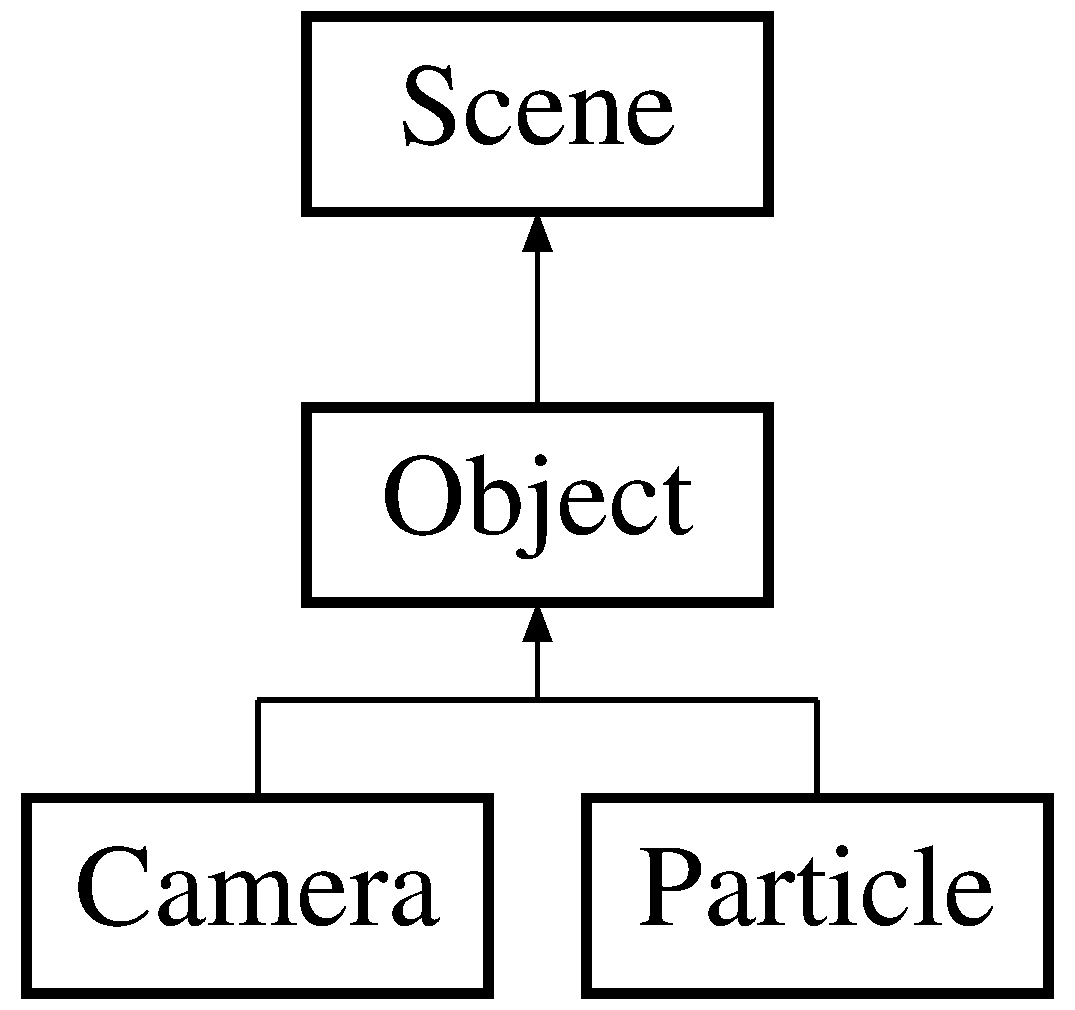
\includegraphics[height=3.000000cm]{class_object}
\end{center}
\end{figure}
\subsection*{Public Types}
\begin{DoxyCompactItemize}
\item 
enum {\bfseries Uniforms} \{ \\*
{\bfseries B\-E\-G\-I\-N}, 
{\bfseries Is\-Textured} = B\-E\-G\-I\-N, 
{\bfseries Object\-C\-T\-M}, 
{\bfseries Morph\-Percentage}, 
\\*
{\bfseries E\-N\-D}
 \}
\item 
\hypertarget{class_object_a79b74057dbc5182b85c9c3ba8480fcf2}{typedef const unsigned int {\bfseries Uniform\-Enum}}\label{class_object_a79b74057dbc5182b85c9c3ba8480fcf2}

\item 
\hypertarget{class_object_a6e19bd8516360bff956408cbae33b878}{typedef std\-::map\\*
$<$ Object\-::\-Uniform\-Enum, \\*
std\-::string $>$ {\bfseries Uniform\-Map}}\label{class_object_a6e19bd8516360bff956408cbae33b878}

\item 
\hypertarget{class_object_ae6a2969ddca87d2c54b7cb1c131a7d60}{typedef enum Object\-::\-Uniforms {\bfseries Uniform}}\label{class_object_ae6a2969ddca87d2c54b7cb1c131a7d60}

\end{DoxyCompactItemize}
\subsection*{Public Member Functions}
\begin{DoxyCompactItemize}
\item 
\hypertarget{class_object_aacf42e81415f32f1f2a105ce29c7c1b9}{{\bfseries Object} (const std\-::string \&\hyperlink{class_object_a24457e0a387492c80594aec7681a2277}{name}, G\-Luint g\-Shader)}\label{class_object_aacf42e81415f32f1f2a105ce29c7c1b9}

\item 
\hypertarget{class_object_a3afa1b9af32b78d81b5de0836c511aeb}{void {\bfseries Draw} (void)}\label{class_object_a3afa1b9af32b78d81b5de0836c511aeb}

\item 
\hypertarget{class_object_a35c89a8eb8a5b742a9025331119bfc7c}{void {\bfseries Buffer} (void)}\label{class_object_a35c89a8eb8a5b742a9025331119bfc7c}

\item 
\hypertarget{class_object_a754f9f36a528f050b25d053ed43015f0}{void {\bfseries Buffer\-Morph\-Only} (void)}\label{class_object_a754f9f36a528f050b25d053ed43015f0}

\item 
\hypertarget{class_object_ac6ccf69d21c4c902c62829c48ef6cf5b}{void {\bfseries Mode} (G\-Lenum new\-\_\-node)}\label{class_object_ac6ccf69d21c4c902c62829c48ef6cf5b}

\item 
\hypertarget{class_object_aa104adfbcc2cae4bd68c053cc3dab721}{void {\bfseries Texture} (const char $\ast$$\ast$filename)}\label{class_object_aa104adfbcc2cae4bd68c053cc3dab721}

\item 
\hypertarget{class_object_a890760dff9df547454112ff84510040c}{const std\-::string \& {\bfseries Name} (void) const }\label{class_object_a890760dff9df547454112ff84510040c}

\item 
\hypertarget{class_object_accde5aa6e8d0d582719e94c414c2341c}{virtual void {\bfseries Link} (Uniform\-Enum which, const std\-::string \&\hyperlink{class_object_a24457e0a387492c80594aec7681a2277}{name})}\label{class_object_accde5aa6e8d0d582719e94c414c2341c}

\item 
\hypertarget{class_object_a34258ee199342d785c29d18c49d54e71}{virtual void {\bfseries send} (Uniform\-Enum which)}\label{class_object_a34258ee199342d785c29d18c49d54e71}

\item 
virtual G\-Luint \hyperlink{class_object_a3dc857b837e8b77ba8a2727233400a5e}{Shader} (void)
\begin{DoxyCompactList}\small\item\em Returns the \hyperlink{class_object}{Object}'s current Shader. \end{DoxyCompactList}\item 
virtual void \hyperlink{class_object_aa52c30bca96800cecba55f446e147859}{Shader} (G\-Luint new\-Shader)
\begin{DoxyCompactList}\small\item\em Sets the shader to be used by this object. \end{DoxyCompactList}\item 
\hypertarget{class_object_ae3226b31c80c9f276ffdee65101c8fa6}{void {\bfseries Animation} (void($\ast$anim\-\_\-func)(\hyperlink{class_trans_cache}{Trans\-Cache} \&arg))}\label{class_object_ae3226b31c80c9f276ffdee65101c8fa6}

\item 
\hypertarget{class_object_ae09449132d3853e179d07d4d6bc0b695}{void {\bfseries Propagate} (void)}\label{class_object_ae09449132d3853e179d07d4d6bc0b695}

\item 
\hyperlink{struct_angel_1_1vec4}{vec4} \hyperlink{class_object_ae10497fea640753a3cb63f739aacc540}{Get\-Position} () const 
\begin{DoxyCompactList}\small\item\em returns the position of the object this makes the lighting implementation much easier... \end{DoxyCompactList}\item 
\hypertarget{class_object_aa60771518c07a0edf5aeee5584a571e0}{\hyperlink{class_object}{Object} $\ast$ {\bfseries get\-Morph\-Target\-Ptr} () const }\label{class_object_aa60771518c07a0edf5aeee5584a571e0}

\item 
\hypertarget{class_object_af4d40010633d77ff47e75d40e3129894}{\hyperlink{class_object}{Object} $\ast$ {\bfseries gen\-Morph\-Target} (G\-Luint)}\label{class_object_af4d40010633d77ff47e75d40e3129894}

\item 
\hypertarget{class_object_a275903685e300433a5120b5558eb9aa1}{float {\bfseries get\-Morph\-Percentage} () const }\label{class_object_a275903685e300433a5120b5558eb9aa1}

\item 
\hypertarget{class_object_aea00114a91aeb779b4f03c7bebaa326e}{void {\bfseries set\-Morph\-Percentage} (const float)}\label{class_object_aea00114a91aeb779b4f03c7bebaa326e}

\item 
\hypertarget{class_object_a98d3f1b9ebb61c3b21e2a59ed267480a}{void {\bfseries destroy\-Morph\-Target} ()}\label{class_object_a98d3f1b9ebb61c3b21e2a59ed267480a}

\item 
\hypertarget{class_object_aae9b55b35a69ba78aa2803b4c8a681b7}{int {\bfseries get\-Number\-Points} ()}\label{class_object_aae9b55b35a69ba78aa2803b4c8a681b7}

\item 
\hypertarget{class_scene_a366b5dec1ecf66a887b4d0dedcd1aa3b}{\hyperlink{class_object}{Object} $\ast$ {\bfseries Add\-Object} (const std\-::string \&obj\-Name, G\-Luint Object\-\_\-\-Shader=0)}\label{class_scene_a366b5dec1ecf66a887b4d0dedcd1aa3b}

\item 
\hypertarget{class_scene_a3bd9fa1058f506c04162b9283e97d20e}{void {\bfseries Del\-Object} (const std\-::string \&obj\-Name)}\label{class_scene_a3bd9fa1058f506c04162b9283e97d20e}

\item 
\hypertarget{class_scene_a43fd3c56db5dc940d1724b9573c9a360}{void {\bfseries Del\-Object} (void)}\label{class_scene_a43fd3c56db5dc940d1724b9573c9a360}

\item 
\hypertarget{class_scene_abdfd15e7987aa261840d5ecc265170df}{void {\bfseries Pop\-Object} (void)}\label{class_scene_abdfd15e7987aa261840d5ecc265170df}

\item 
\hypertarget{class_scene_a82759ded1f6f87a91b8d10ed87501958}{void \hyperlink{class_scene_a82759ded1f6f87a91b8d10ed87501958}{Destroy\-Object} (void)}\label{class_scene_a82759ded1f6f87a91b8d10ed87501958}

\begin{DoxyCompactList}\small\item\em Completely remove this object and all his children. \end{DoxyCompactList}\item 
\hypertarget{class_scene_a70fcdad192a4c6ff508125de8af6cf4d}{\hyperlink{class_object}{Object} $\ast$ {\bfseries next} (void)}\label{class_scene_a70fcdad192a4c6ff508125de8af6cf4d}

\item 
\hypertarget{class_scene_ac852d5d763eb35b4908c9aa7ea54d1ae}{\hyperlink{class_object}{Object} $\ast$ {\bfseries prev} (void)}\label{class_scene_ac852d5d763eb35b4908c9aa7ea54d1ae}

\item 
\hypertarget{class_scene_ad0ea1a6bcf7815c63988bd937f06eb23}{\hyperlink{class_object}{Object} $\ast$ {\bfseries active} (void) const }\label{class_scene_ad0ea1a6bcf7815c63988bd937f06eb23}

\item 
\hypertarget{class_scene_ae9b69d8db8a46991017635f22e45baad}{\hyperlink{class_object}{Object} $\ast$ {\bfseries operator\mbox{[}$\,$\mbox{]}} (const std\-::string \&objname)}\label{class_scene_ae9b69d8db8a46991017635f22e45baad}

\end{DoxyCompactItemize}
\subsection*{Public Attributes}
\begin{DoxyCompactItemize}
\item 
\hypertarget{class_object_a8dec70177d147f59ba10c9eba8e9191b}{std\-::vector$<$ \hyperlink{struct_angel_1_1vec4}{Angel\-::vec4} $>$ {\bfseries points}}\label{class_object_a8dec70177d147f59ba10c9eba8e9191b}

\item 
\hypertarget{class_object_ad541a7bb180e24f59d752cc6d7f8c7e8}{std\-::vector$<$ \hyperlink{struct_angel_1_1vec3}{Angel\-::vec3} $>$ {\bfseries normals}}\label{class_object_ad541a7bb180e24f59d752cc6d7f8c7e8}

\item 
\hypertarget{class_object_a9b2fb19d129ad79407f9af0eea05b96c}{std\-::vector$<$ unsigned int $>$ {\bfseries indices}}\label{class_object_a9b2fb19d129ad79407f9af0eea05b96c}

\item 
\hypertarget{class_object_a4de4c1e2c4b621efb6f5d1b398ac6835}{std\-::vector$<$ \hyperlink{struct_angel_1_1vec4}{Angel\-::vec4} $>$ {\bfseries colors}}\label{class_object_a4de4c1e2c4b621efb6f5d1b398ac6835}

\item 
\hypertarget{class_object_a6d6c58ccb93f7a2bd7439d081134aaa0}{std\-::vector$<$ \hyperlink{struct_angel_1_1vec2}{Angel\-::vec2} $>$ {\bfseries texcoords}}\label{class_object_a6d6c58ccb93f7a2bd7439d081134aaa0}

\item 
\hypertarget{class_object_a1bb011587e4fa6e69984d5679546b1cb}{\hyperlink{class_trans_cache}{Trans\-Cache} {\bfseries trans}}\label{class_object_a1bb011587e4fa6e69984d5679546b1cb}

\end{DoxyCompactItemize}
\subsection*{Protected Member Functions}
\begin{DoxyCompactItemize}
\item 
void \hyperlink{class_scene_a8bbe0e5b1bfc71034b18e240e86aa285}{Delete\-Object} (\hyperlink{class_object}{Object} $\ast$obj)
\begin{DoxyCompactList}\small\item\em Delete\-Object is the actual implementation function that will remove an \hyperlink{class_object}{Object} from the \hyperlink{class_scene}{Scene} list and \hyperlink{class_scene}{Scene} map, then free the object. \end{DoxyCompactList}\item 
\hypertarget{class_scene_ae8d51ddc196248a7cbd1f3640851dbd4}{void {\bfseries Insert\-Object} (const std\-::string \hyperlink{class_object_a24457e0a387492c80594aec7681a2277}{name}, \hyperlink{class_object}{Object} $\ast$obj)}\label{class_scene_ae8d51ddc196248a7cbd1f3640851dbd4}

\end{DoxyCompactItemize}
\subsection*{Protected Attributes}
\begin{DoxyCompactItemize}
\item 
std\-::string \hyperlink{class_object_a24457e0a387492c80594aec7681a2277}{name}
\begin{DoxyCompactList}\small\item\em name is used as an identifying handle for the object. \end{DoxyCompactList}\item 
G\-Luint \hyperlink{class_object_a66190fee29d03d6478516686cbd01eb8}{vao}
\begin{DoxyCompactList}\small\item\em Vertex Array \hyperlink{class_object}{Object} handle identifying our buffers/object. \end{DoxyCompactList}\item 
\hypertarget{class_object_a29de966ce95d96e19262c4f10f0b4276}{G\-Luint \hyperlink{class_object_a29de966ce95d96e19262c4f10f0b4276}{buffer} \mbox{[}N\-U\-M\-\_\-\-B\-U\-F\-F\-E\-R\-S\mbox{]}}\label{class_object_a29de966ce95d96e19262c4f10f0b4276}

\begin{DoxyCompactList}\small\item\em Handles to our buffers (Vertices, Tex\-U\-Vs, etc.) \end{DoxyCompactList}\item 
G\-Lenum \hyperlink{class_object_a82764b385767d989f27d301ab206acb8}{draw\-\_\-mode}
\begin{DoxyCompactList}\small\item\em Drawing mode for this object. \end{DoxyCompactList}\item 
\hypertarget{class_object_a2bbbe3a5b33cbcfc4c536b49d470a6b8}{bool \hyperlink{class_object_a2bbbe3a5b33cbcfc4c536b49d470a6b8}{is\-Textured}}\label{class_object_a2bbbe3a5b33cbcfc4c536b49d470a6b8}

\begin{DoxyCompactList}\small\item\em Is this object textured? \end{DoxyCompactList}\item 
\hypertarget{class_object_ac5ca00d03136434b93ae7d00808554c7}{float \hyperlink{class_object_ac5ca00d03136434b93ae7d00808554c7}{morph\-Percentage}}\label{class_object_ac5ca00d03136434b93ae7d00808554c7}

\begin{DoxyCompactList}\small\item\em Morphing/\-Tweening Things. \end{DoxyCompactList}\item 
\hypertarget{class_object_acfc4dec49d5d273910c3a1af2b3adfcd}{\hyperlink{class_object}{Object} $\ast$ {\bfseries morph\-Target}}\label{class_object_acfc4dec49d5d273910c3a1af2b3adfcd}

\item 
\hypertarget{class_object_a6378d0b0eeec23045ae2a5245e42bf13}{std\-::map$<$ Object\-::\-Uniform\-Enum, \\*
std\-::string $>$ {\bfseries \-\_\-uniform\-Map}}\label{class_object_a6378d0b0eeec23045ae2a5245e42bf13}

\item 
std\-::vector$<$ G\-Lint $>$ \hyperlink{class_object_acd6c7021617ea334915a1525f9519bc5}{handles}
\begin{DoxyCompactList}\small\item\em Handles to Uniforms on the shader. \end{DoxyCompactList}\item 
\hypertarget{class_scene_acdd0123ca6b2d64d8d447bb485b235fc}{std\-::list$<$ \hyperlink{class_object}{Object} $\ast$ $>$ {\bfseries \-\_\-list}}\label{class_scene_acdd0123ca6b2d64d8d447bb485b235fc}

\item 
\hypertarget{class_scene_a8bd5d86484a12255b26b92b6cbf8d29a}{std\-::map$<$ std\-::string, \hyperlink{class_object}{Object} $\ast$ $>$ {\bfseries \-\_\-map}}\label{class_scene_a8bd5d86484a12255b26b92b6cbf8d29a}

\item 
\hypertarget{class_scene_ae87ca5350fcc595f3f15a4fd3c39f3d9}{std\-::list$<$ \hyperlink{class_object}{Object} $\ast$ $>$\-::iterator {\bfseries \-\_\-current\-Obj}}\label{class_scene_ae87ca5350fcc595f3f15a4fd3c39f3d9}

\item 
\hypertarget{class_scene_a8f9bdd8ec5edb1f414fbd314a36e2724}{G\-Luint {\bfseries \-\_\-g\-Shader}}\label{class_scene_a8f9bdd8ec5edb1f414fbd314a36e2724}

\end{DoxyCompactItemize}
\subsection*{Private Types}
\begin{DoxyCompactItemize}
\item 
enum {\bfseries buffer\-Type} \{ \\*
{\bfseries V\-E\-R\-T\-I\-C\-E\-S}, 
{\bfseries N\-O\-R\-M\-A\-L\-S}, 
{\bfseries I\-N\-D\-I\-C\-E\-S}, 
{\bfseries C\-O\-L\-O\-R\-S}, 
\\*
{\bfseries T\-E\-X\-C\-O\-O\-R\-D\-S}, 
{\bfseries V\-E\-R\-T\-I\-C\-E\-S\-\_\-\-M\-O\-R\-P\-H}, 
{\bfseries N\-O\-R\-M\-A\-L\-S\-\_\-\-M\-O\-R\-P\-H}, 
{\bfseries C\-O\-L\-O\-R\-S\-\_\-\-M\-O\-R\-P\-H}, 
\\*
{\bfseries N\-U\-M\-\_\-\-B\-U\-F\-F\-E\-R\-S}
 \}
\end{DoxyCompactItemize}


\subsection{Detailed Description}


Definition at line 16 of file Object.\-hpp.



\subsection{Member Function Documentation}
\hypertarget{class_scene_a8bbe0e5b1bfc71034b18e240e86aa285}{\index{Object@{Object}!Delete\-Object@{Delete\-Object}}
\index{Delete\-Object@{Delete\-Object}!Object@{Object}}
\subsubsection[{Delete\-Object}]{\setlength{\rightskip}{0pt plus 5cm}void Scene\-::\-Delete\-Object (
\begin{DoxyParamCaption}
\item[{{\bf Object} $\ast$}]{obj}
\end{DoxyParamCaption}
)\hspace{0.3cm}{\ttfamily [protected]}, {\ttfamily [inherited]}}}\label{class_scene_a8bbe0e5b1bfc71034b18e240e86aa285}


Delete\-Object is the actual implementation function that will remove an \hyperlink{class_object}{Object} from the \hyperlink{class_scene}{Scene} list and \hyperlink{class_scene}{Scene} map, then free the object. 


\begin{DoxyParams}{Parameters}
{\em obj} & The pointer to the object to free. \\
\hline
\end{DoxyParams}


Definition at line 76 of file Scene.\-cpp.

\hypertarget{class_object_ae10497fea640753a3cb63f739aacc540}{\index{Object@{Object}!Get\-Position@{Get\-Position}}
\index{Get\-Position@{Get\-Position}!Object@{Object}}
\subsubsection[{Get\-Position}]{\setlength{\rightskip}{0pt plus 5cm}{\bf vec4} Object\-::\-Get\-Position (
\begin{DoxyParamCaption}
{}
\end{DoxyParamCaption}
) const}}\label{class_object_ae10497fea640753a3cb63f739aacc540}


returns the position of the object this makes the lighting implementation much easier... 

for this semester. 

Definition at line 497 of file Object.\-cpp.

\hypertarget{class_object_a3dc857b837e8b77ba8a2727233400a5e}{\index{Object@{Object}!Shader@{Shader}}
\index{Shader@{Shader}!Object@{Object}}
\subsubsection[{Shader}]{\setlength{\rightskip}{0pt plus 5cm}G\-Luint Object\-::\-Shader (
\begin{DoxyParamCaption}
\item[{void}]{}
\end{DoxyParamCaption}
)\hspace{0.3cm}{\ttfamily [virtual]}}}\label{class_object_a3dc857b837e8b77ba8a2727233400a5e}


Returns the \hyperlink{class_object}{Object}'s current Shader. 

Defined because C++ will not let you overload an overrided function, without re-\/overloading it in the derived class.

\begin{DoxyReturn}{Returns}
a G\-Luint handle to the shader program used by this \hyperlink{class_object}{Object}. 
\end{DoxyReturn}


Definition at line 269 of file Object.\-cpp.

\hypertarget{class_object_aa52c30bca96800cecba55f446e147859}{\index{Object@{Object}!Shader@{Shader}}
\index{Shader@{Shader}!Object@{Object}}
\subsubsection[{Shader}]{\setlength{\rightskip}{0pt plus 5cm}void Object\-::\-Shader (
\begin{DoxyParamCaption}
\item[{G\-Luint}]{new\-Shader}
\end{DoxyParamCaption}
)\hspace{0.3cm}{\ttfamily [virtual]}}}\label{class_object_aa52c30bca96800cecba55f446e147859}


Sets the shader to be used by this object. 

Triggers a query of the shader program, for the locations of the Uniform locations that the object needs.


\begin{DoxyParams}{Parameters}
{\em new\-Shader} & a G\-Luint handle to the shader program to use.\\
\hline
\end{DoxyParams}
\begin{DoxyReturn}{Returns}
None. 
\end{DoxyReturn}


Reimplemented from \hyperlink{class_scene_a7137a7302c21ac4dd44e746bfb6f7cf8}{Scene}.



Definition at line 246 of file Object.\-cpp.



\subsection{Member Data Documentation}
\hypertarget{class_object_a82764b385767d989f27d301ab206acb8}{\index{Object@{Object}!draw\-\_\-mode@{draw\-\_\-mode}}
\index{draw\-\_\-mode@{draw\-\_\-mode}!Object@{Object}}
\subsubsection[{draw\-\_\-mode}]{\setlength{\rightskip}{0pt plus 5cm}G\-Lenum Object\-::draw\-\_\-mode\hspace{0.3cm}{\ttfamily [protected]}}}\label{class_object_a82764b385767d989f27d301ab206acb8}


Drawing mode for this object. 

G\-L\-\_\-\-T\-R\-I\-A\-N\-G\-L\-E\-S, G\-L\-\_\-\-L\-I\-N\-E\-\_\-\-L\-O\-O\-P, etc. 

Definition at line 95 of file Object.\-hpp.

\hypertarget{class_object_acd6c7021617ea334915a1525f9519bc5}{\index{Object@{Object}!handles@{handles}}
\index{handles@{handles}!Object@{Object}}
\subsubsection[{handles}]{\setlength{\rightskip}{0pt plus 5cm}std\-::vector$<$ G\-Lint $>$ Object\-::handles\hspace{0.3cm}{\ttfamily [protected]}}}\label{class_object_acd6c7021617ea334915a1525f9519bc5}


Handles to Uniforms on the shader. 

Private to allow derived classes to extend it as needed. 

Definition at line 114 of file Object.\-hpp.

\hypertarget{class_object_a24457e0a387492c80594aec7681a2277}{\index{Object@{Object}!name@{name}}
\index{name@{name}!Object@{Object}}
\subsubsection[{name}]{\setlength{\rightskip}{0pt plus 5cm}std\-::string Object\-::name\hspace{0.3cm}{\ttfamily [protected]}}}\label{class_object_a24457e0a387492c80594aec7681a2277}


name is used as an identifying handle for the object. 



Definition at line 86 of file Object.\-hpp.

\hypertarget{class_object_a66190fee29d03d6478516686cbd01eb8}{\index{Object@{Object}!vao@{vao}}
\index{vao@{vao}!Object@{Object}}
\subsubsection[{vao}]{\setlength{\rightskip}{0pt plus 5cm}G\-Luint Object\-::vao\hspace{0.3cm}{\ttfamily [protected]}}}\label{class_object_a66190fee29d03d6478516686cbd01eb8}


Vertex Array \hyperlink{class_object}{Object} handle identifying our buffers/object. 



Definition at line 89 of file Object.\-hpp.



The documentation for this class was generated from the following files\-:\begin{DoxyCompactItemize}
\item 
Object.\-hpp\item 
Object.\-cpp\end{DoxyCompactItemize}

\hypertarget{class_particle}{\section{Particle Class Reference}
\label{class_particle}\index{Particle@{Particle}}
}


todo  




{\ttfamily \#include $<$Particle.\-hpp$>$}

Inheritance diagram for Particle\-:\begin{figure}[H]
\begin{center}
\leavevmode
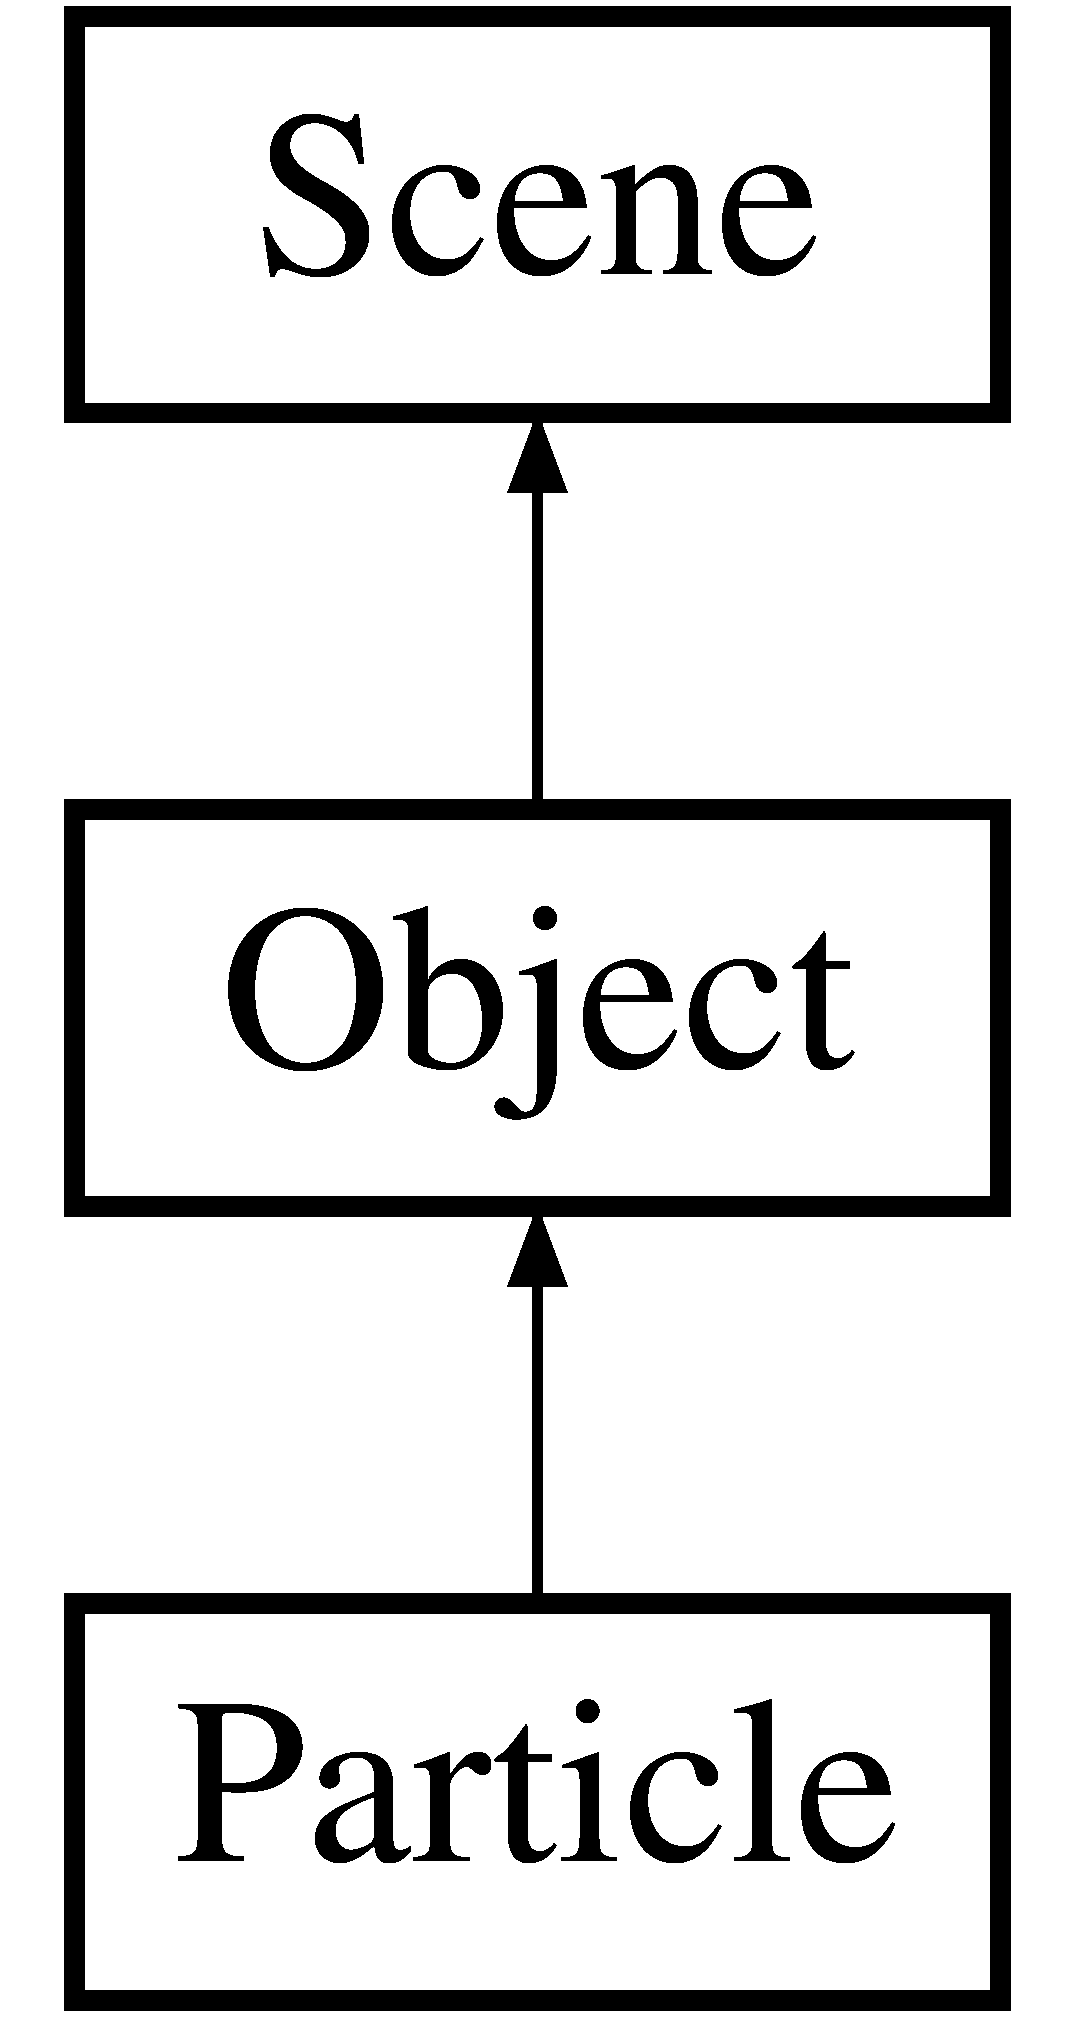
\includegraphics[height=3.000000cm]{class_particle}
\end{center}
\end{figure}
\subsection*{Public Types}
\begin{DoxyCompactItemize}
\item 
enum {\bfseries Uniforms} \{ \\*
{\bfseries B\-E\-G\-I\-N}, 
{\bfseries Is\-Textured} = B\-E\-G\-I\-N, 
{\bfseries Object\-C\-T\-M}, 
{\bfseries Morph\-Percentage}, 
\\*
{\bfseries E\-N\-D}
 \}
\item 
\hypertarget{class_object_a79b74057dbc5182b85c9c3ba8480fcf2}{typedef const unsigned int {\bfseries Uniform\-Enum}}\label{class_object_a79b74057dbc5182b85c9c3ba8480fcf2}

\item 
\hypertarget{class_object_a6e19bd8516360bff956408cbae33b878}{typedef std\-::map\\*
$<$ Object\-::\-Uniform\-Enum, \\*
std\-::string $>$ {\bfseries Uniform\-Map}}\label{class_object_a6e19bd8516360bff956408cbae33b878}

\item 
\hypertarget{class_object_ae6a2969ddca87d2c54b7cb1c131a7d60}{typedef enum Object\-::\-Uniforms {\bfseries Uniform}}\label{class_object_ae6a2969ddca87d2c54b7cb1c131a7d60}

\end{DoxyCompactItemize}
\subsection*{Public Member Functions}
\begin{DoxyCompactItemize}
\item 
\hypertarget{class_particle_afcdc6f92de4e525a67617fe9fee6ae5d}{{\bfseries Particle} (\hyperlink{struct_angel_1_1vec4}{vec4} init\-Pos, \hyperlink{struct_angel_1_1vec3}{vec3} init\-Scale, \hyperlink{struct_angel_1_1vec3}{vec3} init\-Vel, float init\-Alpha, \hyperlink{struct_angel_1_1vec4}{vec4} init\-Color, float init\-Lifespan, float init\-Spin, string init\-Tex)}\label{class_particle_afcdc6f92de4e525a67617fe9fee6ae5d}

\item 
\hypertarget{class_particle_a686aad22bf7a80a089e117bbc7f4b738}{void {\bfseries update} ()}\label{class_particle_a686aad22bf7a80a089e117bbc7f4b738}

\item 
\hypertarget{class_particle_aabc36f29b35e0e1e5c6d6fb926bb7bbb}{void {\bfseries set\-Pos} (\hyperlink{struct_angel_1_1vec4}{vec4} new\-Pos)}\label{class_particle_aabc36f29b35e0e1e5c6d6fb926bb7bbb}

\item 
\hypertarget{class_particle_a1cdeee73a5eb04f48c0002f7136852ff}{void {\bfseries set\-Scale} (\hyperlink{struct_angel_1_1vec3}{vec3} new\-Scale)}\label{class_particle_a1cdeee73a5eb04f48c0002f7136852ff}

\item 
\hypertarget{class_particle_ac77b501936d44053585151c83b66ba22}{void {\bfseries set\-Vel} (\hyperlink{struct_angel_1_1vec3}{vec3} new\-Vel)}\label{class_particle_ac77b501936d44053585151c83b66ba22}

\item 
\hypertarget{class_particle_a3d339beee1c13eb3d1eed69d14715106}{void {\bfseries set\-Alpha} (float new\-Alpha)}\label{class_particle_a3d339beee1c13eb3d1eed69d14715106}

\item 
\hypertarget{class_particle_a8dbaf5f085a47c834c02f0531ccdbae1}{void {\bfseries set\-Color} (\hyperlink{struct_angel_1_1vec4}{vec4} new\-Color)}\label{class_particle_a8dbaf5f085a47c834c02f0531ccdbae1}

\item 
\hypertarget{class_particle_a2f59e88a58a6c6ea766ab4c94c75c2b3}{void {\bfseries set\-Lifespan} (float new\-Lifespan)}\label{class_particle_a2f59e88a58a6c6ea766ab4c94c75c2b3}

\item 
\hypertarget{class_particle_ac0cd12e63886b12d2b99549ecb552838}{void {\bfseries set\-Spin} (float new\-Spin)}\label{class_particle_ac0cd12e63886b12d2b99549ecb552838}

\item 
\hypertarget{class_particle_a5a387ad04e530af85dcd64763282d3a0}{void {\bfseries set\-Tex\-File} (string new\-Filename)}\label{class_particle_a5a387ad04e530af85dcd64763282d3a0}

\item 
\hypertarget{class_object_a3afa1b9af32b78d81b5de0836c511aeb}{void {\bfseries Draw} (void)}\label{class_object_a3afa1b9af32b78d81b5de0836c511aeb}

\item 
\hypertarget{class_object_a35c89a8eb8a5b742a9025331119bfc7c}{void {\bfseries Buffer} (void)}\label{class_object_a35c89a8eb8a5b742a9025331119bfc7c}

\item 
\hypertarget{class_object_a754f9f36a528f050b25d053ed43015f0}{void {\bfseries Buffer\-Morph\-Only} (void)}\label{class_object_a754f9f36a528f050b25d053ed43015f0}

\item 
\hypertarget{class_object_ac6ccf69d21c4c902c62829c48ef6cf5b}{void {\bfseries Mode} (G\-Lenum new\-\_\-node)}\label{class_object_ac6ccf69d21c4c902c62829c48ef6cf5b}

\item 
\hypertarget{class_object_aa104adfbcc2cae4bd68c053cc3dab721}{void {\bfseries Texture} (const char $\ast$$\ast$filename)}\label{class_object_aa104adfbcc2cae4bd68c053cc3dab721}

\item 
\hypertarget{class_object_a890760dff9df547454112ff84510040c}{const std\-::string \& {\bfseries Name} (void) const }\label{class_object_a890760dff9df547454112ff84510040c}

\item 
\hypertarget{class_object_accde5aa6e8d0d582719e94c414c2341c}{virtual void {\bfseries Link} (Uniform\-Enum which, const std\-::string \&\hyperlink{class_object_a24457e0a387492c80594aec7681a2277}{name})}\label{class_object_accde5aa6e8d0d582719e94c414c2341c}

\item 
\hypertarget{class_object_a34258ee199342d785c29d18c49d54e71}{virtual void {\bfseries send} (Uniform\-Enum which)}\label{class_object_a34258ee199342d785c29d18c49d54e71}

\item 
virtual G\-Luint \hyperlink{class_object_a3dc857b837e8b77ba8a2727233400a5e}{Shader} (void)
\begin{DoxyCompactList}\small\item\em Returns the \hyperlink{class_object}{Object}'s current Shader. \end{DoxyCompactList}\item 
virtual void \hyperlink{class_object_aa52c30bca96800cecba55f446e147859}{Shader} (G\-Luint new\-Shader)
\begin{DoxyCompactList}\small\item\em Sets the shader to be used by this object. \end{DoxyCompactList}\item 
\hypertarget{class_object_ae3226b31c80c9f276ffdee65101c8fa6}{void {\bfseries Animation} (void($\ast$anim\-\_\-func)(\hyperlink{class_trans_cache}{Trans\-Cache} \&arg))}\label{class_object_ae3226b31c80c9f276ffdee65101c8fa6}

\item 
\hypertarget{class_object_ae09449132d3853e179d07d4d6bc0b695}{void {\bfseries Propagate} (void)}\label{class_object_ae09449132d3853e179d07d4d6bc0b695}

\item 
\hyperlink{struct_angel_1_1vec4}{vec4} \hyperlink{class_object_ae10497fea640753a3cb63f739aacc540}{Get\-Position} () const 
\begin{DoxyCompactList}\small\item\em returns the position of the object this makes the lighting implementation much easier... \end{DoxyCompactList}\item 
\hypertarget{class_object_aa60771518c07a0edf5aeee5584a571e0}{\hyperlink{class_object}{Object} $\ast$ {\bfseries get\-Morph\-Target\-Ptr} () const }\label{class_object_aa60771518c07a0edf5aeee5584a571e0}

\item 
\hypertarget{class_object_af4d40010633d77ff47e75d40e3129894}{\hyperlink{class_object}{Object} $\ast$ {\bfseries gen\-Morph\-Target} (G\-Luint)}\label{class_object_af4d40010633d77ff47e75d40e3129894}

\item 
\hypertarget{class_object_a275903685e300433a5120b5558eb9aa1}{float {\bfseries get\-Morph\-Percentage} () const }\label{class_object_a275903685e300433a5120b5558eb9aa1}

\item 
\hypertarget{class_object_aea00114a91aeb779b4f03c7bebaa326e}{void {\bfseries set\-Morph\-Percentage} (const float)}\label{class_object_aea00114a91aeb779b4f03c7bebaa326e}

\item 
\hypertarget{class_object_a98d3f1b9ebb61c3b21e2a59ed267480a}{void {\bfseries destroy\-Morph\-Target} ()}\label{class_object_a98d3f1b9ebb61c3b21e2a59ed267480a}

\item 
\hypertarget{class_object_aae9b55b35a69ba78aa2803b4c8a681b7}{int {\bfseries get\-Number\-Points} ()}\label{class_object_aae9b55b35a69ba78aa2803b4c8a681b7}

\item 
\hypertarget{class_scene_a366b5dec1ecf66a887b4d0dedcd1aa3b}{\hyperlink{class_object}{Object} $\ast$ {\bfseries Add\-Object} (const std\-::string \&obj\-Name, G\-Luint Object\-\_\-\-Shader=0)}\label{class_scene_a366b5dec1ecf66a887b4d0dedcd1aa3b}

\item 
\hypertarget{class_scene_a3bd9fa1058f506c04162b9283e97d20e}{void {\bfseries Del\-Object} (const std\-::string \&obj\-Name)}\label{class_scene_a3bd9fa1058f506c04162b9283e97d20e}

\item 
\hypertarget{class_scene_a43fd3c56db5dc940d1724b9573c9a360}{void {\bfseries Del\-Object} (void)}\label{class_scene_a43fd3c56db5dc940d1724b9573c9a360}

\item 
\hypertarget{class_scene_abdfd15e7987aa261840d5ecc265170df}{void {\bfseries Pop\-Object} (void)}\label{class_scene_abdfd15e7987aa261840d5ecc265170df}

\item 
\hypertarget{class_scene_a82759ded1f6f87a91b8d10ed87501958}{void \hyperlink{class_scene_a82759ded1f6f87a91b8d10ed87501958}{Destroy\-Object} (void)}\label{class_scene_a82759ded1f6f87a91b8d10ed87501958}

\begin{DoxyCompactList}\small\item\em Completely remove this object and all his children. \end{DoxyCompactList}\item 
\hypertarget{class_scene_a70fcdad192a4c6ff508125de8af6cf4d}{\hyperlink{class_object}{Object} $\ast$ {\bfseries next} (void)}\label{class_scene_a70fcdad192a4c6ff508125de8af6cf4d}

\item 
\hypertarget{class_scene_ac852d5d763eb35b4908c9aa7ea54d1ae}{\hyperlink{class_object}{Object} $\ast$ {\bfseries prev} (void)}\label{class_scene_ac852d5d763eb35b4908c9aa7ea54d1ae}

\item 
\hypertarget{class_scene_ad0ea1a6bcf7815c63988bd937f06eb23}{\hyperlink{class_object}{Object} $\ast$ {\bfseries active} (void) const }\label{class_scene_ad0ea1a6bcf7815c63988bd937f06eb23}

\item 
\hypertarget{class_scene_ae9b69d8db8a46991017635f22e45baad}{\hyperlink{class_object}{Object} $\ast$ {\bfseries operator\mbox{[}$\,$\mbox{]}} (const std\-::string \&objname)}\label{class_scene_ae9b69d8db8a46991017635f22e45baad}

\end{DoxyCompactItemize}
\subsection*{Public Attributes}
\begin{DoxyCompactItemize}
\item 
\hypertarget{class_object_a8dec70177d147f59ba10c9eba8e9191b}{std\-::vector$<$ \hyperlink{struct_angel_1_1vec4}{Angel\-::vec4} $>$ {\bfseries points}}\label{class_object_a8dec70177d147f59ba10c9eba8e9191b}

\item 
\hypertarget{class_object_ad541a7bb180e24f59d752cc6d7f8c7e8}{std\-::vector$<$ \hyperlink{struct_angel_1_1vec3}{Angel\-::vec3} $>$ {\bfseries normals}}\label{class_object_ad541a7bb180e24f59d752cc6d7f8c7e8}

\item 
\hypertarget{class_object_a9b2fb19d129ad79407f9af0eea05b96c}{std\-::vector$<$ unsigned int $>$ {\bfseries indices}}\label{class_object_a9b2fb19d129ad79407f9af0eea05b96c}

\item 
\hypertarget{class_object_a4de4c1e2c4b621efb6f5d1b398ac6835}{std\-::vector$<$ \hyperlink{struct_angel_1_1vec4}{Angel\-::vec4} $>$ {\bfseries colors}}\label{class_object_a4de4c1e2c4b621efb6f5d1b398ac6835}

\item 
\hypertarget{class_object_a6d6c58ccb93f7a2bd7439d081134aaa0}{std\-::vector$<$ \hyperlink{struct_angel_1_1vec2}{Angel\-::vec2} $>$ {\bfseries texcoords}}\label{class_object_a6d6c58ccb93f7a2bd7439d081134aaa0}

\item 
\hypertarget{class_object_a1bb011587e4fa6e69984d5679546b1cb}{\hyperlink{class_trans_cache}{Trans\-Cache} {\bfseries trans}}\label{class_object_a1bb011587e4fa6e69984d5679546b1cb}

\end{DoxyCompactItemize}
\subsection*{Protected Member Functions}
\begin{DoxyCompactItemize}
\item 
void \hyperlink{class_scene_a8bbe0e5b1bfc71034b18e240e86aa285}{Delete\-Object} (\hyperlink{class_object}{Object} $\ast$obj)
\begin{DoxyCompactList}\small\item\em Delete\-Object is the actual implementation function that will remove an \hyperlink{class_object}{Object} from the \hyperlink{class_scene}{Scene} list and \hyperlink{class_scene}{Scene} map, then free the object. \end{DoxyCompactList}\item 
\hypertarget{class_scene_ae8d51ddc196248a7cbd1f3640851dbd4}{void {\bfseries Insert\-Object} (const std\-::string \hyperlink{class_object_a24457e0a387492c80594aec7681a2277}{name}, \hyperlink{class_object}{Object} $\ast$obj)}\label{class_scene_ae8d51ddc196248a7cbd1f3640851dbd4}

\end{DoxyCompactItemize}
\subsection*{Protected Attributes}
\begin{DoxyCompactItemize}
\item 
std\-::string \hyperlink{class_object_a24457e0a387492c80594aec7681a2277}{name}
\begin{DoxyCompactList}\small\item\em name is used as an identifying handle for the object. \end{DoxyCompactList}\item 
G\-Luint \hyperlink{class_object_a66190fee29d03d6478516686cbd01eb8}{vao}
\begin{DoxyCompactList}\small\item\em Vertex Array \hyperlink{class_object}{Object} handle identifying our buffers/object. \end{DoxyCompactList}\item 
\hypertarget{class_object_a29de966ce95d96e19262c4f10f0b4276}{G\-Luint \hyperlink{class_object_a29de966ce95d96e19262c4f10f0b4276}{buffer} \mbox{[}N\-U\-M\-\_\-\-B\-U\-F\-F\-E\-R\-S\mbox{]}}\label{class_object_a29de966ce95d96e19262c4f10f0b4276}

\begin{DoxyCompactList}\small\item\em Handles to our buffers (Vertices, Tex\-U\-Vs, etc.) \end{DoxyCompactList}\item 
G\-Lenum \hyperlink{class_object_a82764b385767d989f27d301ab206acb8}{draw\-\_\-mode}
\begin{DoxyCompactList}\small\item\em Drawing mode for this object. \end{DoxyCompactList}\item 
\hypertarget{class_object_a2bbbe3a5b33cbcfc4c536b49d470a6b8}{bool \hyperlink{class_object_a2bbbe3a5b33cbcfc4c536b49d470a6b8}{is\-Textured}}\label{class_object_a2bbbe3a5b33cbcfc4c536b49d470a6b8}

\begin{DoxyCompactList}\small\item\em Is this object textured? \end{DoxyCompactList}\item 
\hypertarget{class_object_ac5ca00d03136434b93ae7d00808554c7}{float \hyperlink{class_object_ac5ca00d03136434b93ae7d00808554c7}{morph\-Percentage}}\label{class_object_ac5ca00d03136434b93ae7d00808554c7}

\begin{DoxyCompactList}\small\item\em Morphing/\-Tweening Things. \end{DoxyCompactList}\item 
\hypertarget{class_object_acfc4dec49d5d273910c3a1af2b3adfcd}{\hyperlink{class_object}{Object} $\ast$ {\bfseries morph\-Target}}\label{class_object_acfc4dec49d5d273910c3a1af2b3adfcd}

\item 
\hypertarget{class_object_a6378d0b0eeec23045ae2a5245e42bf13}{std\-::map$<$ Object\-::\-Uniform\-Enum, \\*
std\-::string $>$ {\bfseries \-\_\-uniform\-Map}}\label{class_object_a6378d0b0eeec23045ae2a5245e42bf13}

\item 
std\-::vector$<$ G\-Lint $>$ \hyperlink{class_object_acd6c7021617ea334915a1525f9519bc5}{handles}
\begin{DoxyCompactList}\small\item\em Handles to Uniforms on the shader. \end{DoxyCompactList}\item 
\hypertarget{class_scene_acdd0123ca6b2d64d8d447bb485b235fc}{std\-::list$<$ \hyperlink{class_object}{Object} $\ast$ $>$ {\bfseries \-\_\-list}}\label{class_scene_acdd0123ca6b2d64d8d447bb485b235fc}

\item 
\hypertarget{class_scene_a8bd5d86484a12255b26b92b6cbf8d29a}{std\-::map$<$ std\-::string, \hyperlink{class_object}{Object} $\ast$ $>$ {\bfseries \-\_\-map}}\label{class_scene_a8bd5d86484a12255b26b92b6cbf8d29a}

\item 
\hypertarget{class_scene_ae87ca5350fcc595f3f15a4fd3c39f3d9}{std\-::list$<$ \hyperlink{class_object}{Object} $\ast$ $>$\-::iterator {\bfseries \-\_\-current\-Obj}}\label{class_scene_ae87ca5350fcc595f3f15a4fd3c39f3d9}

\item 
\hypertarget{class_scene_a8f9bdd8ec5edb1f414fbd314a36e2724}{G\-Luint {\bfseries \-\_\-g\-Shader}}\label{class_scene_a8f9bdd8ec5edb1f414fbd314a36e2724}

\end{DoxyCompactItemize}
\subsection*{Private Attributes}
\begin{DoxyCompactItemize}
\item 
\hypertarget{class_particle_a3d51791a544fb2cbf2e93531b3626132}{\hyperlink{struct_angel_1_1vec4}{vec4} {\bfseries m\-Pos}}\label{class_particle_a3d51791a544fb2cbf2e93531b3626132}

\item 
\hypertarget{class_particle_ad18c1ecffb2e5d032732d4cd058bb986}{\hyperlink{struct_angel_1_1vec3}{vec3} {\bfseries m\-Scale}}\label{class_particle_ad18c1ecffb2e5d032732d4cd058bb986}

\item 
\hypertarget{class_particle_a4cd8cbbc5b05126133df8246611339f2}{\hyperlink{struct_angel_1_1vec3}{vec3} {\bfseries m\-Vel}}\label{class_particle_a4cd8cbbc5b05126133df8246611339f2}

\item 
\hypertarget{class_particle_a14af67b37c2acfcbaffcc766b660a5f6}{float {\bfseries alpha}}\label{class_particle_a14af67b37c2acfcbaffcc766b660a5f6}

\item 
\hypertarget{class_particle_a3ec1cf194290dd222d3894e30a111db0}{\hyperlink{struct_angel_1_1vec4}{vec4} {\bfseries blend\-Color}}\label{class_particle_a3ec1cf194290dd222d3894e30a111db0}

\item 
\hypertarget{class_particle_a08108b2a0a2c0ec96f235510cc9aa0a2}{float {\bfseries lifespan}}\label{class_particle_a08108b2a0a2c0ec96f235510cc9aa0a2}

\item 
\hypertarget{class_particle_a73e6af7e8d30f1cbf570cc93fbe6529e}{float {\bfseries spin}}\label{class_particle_a73e6af7e8d30f1cbf570cc93fbe6529e}

\item 
\hypertarget{class_particle_a639147e87ea9fd39b04ac3bafb6ff97b}{string {\bfseries tex\-Filename}}\label{class_particle_a639147e87ea9fd39b04ac3bafb6ff97b}

\end{DoxyCompactItemize}


\subsection{Detailed Description}
todo 

\begin{DoxyAuthor}{Author}
Nick Ver Voort, \href{mailto:nicholas_vervoort@student.uml.edu}{\tt nicholas\-\_\-vervoort@student.\-uml.\-edu} 
\end{DoxyAuthor}
\begin{DoxySince}{Since}
23 Feb 2013 
\end{DoxySince}


Definition at line 22 of file Particle.\-hpp.



\subsection{Member Function Documentation}
\hypertarget{class_scene_a8bbe0e5b1bfc71034b18e240e86aa285}{\index{Particle@{Particle}!Delete\-Object@{Delete\-Object}}
\index{Delete\-Object@{Delete\-Object}!Particle@{Particle}}
\subsubsection[{Delete\-Object}]{\setlength{\rightskip}{0pt plus 5cm}void Scene\-::\-Delete\-Object (
\begin{DoxyParamCaption}
\item[{{\bf Object} $\ast$}]{obj}
\end{DoxyParamCaption}
)\hspace{0.3cm}{\ttfamily [protected]}, {\ttfamily [inherited]}}}\label{class_scene_a8bbe0e5b1bfc71034b18e240e86aa285}


Delete\-Object is the actual implementation function that will remove an \hyperlink{class_object}{Object} from the \hyperlink{class_scene}{Scene} list and \hyperlink{class_scene}{Scene} map, then free the object. 


\begin{DoxyParams}{Parameters}
{\em obj} & The pointer to the object to free. \\
\hline
\end{DoxyParams}


Definition at line 76 of file Scene.\-cpp.

\hypertarget{class_object_ae10497fea640753a3cb63f739aacc540}{\index{Particle@{Particle}!Get\-Position@{Get\-Position}}
\index{Get\-Position@{Get\-Position}!Particle@{Particle}}
\subsubsection[{Get\-Position}]{\setlength{\rightskip}{0pt plus 5cm}{\bf vec4} Object\-::\-Get\-Position (
\begin{DoxyParamCaption}
{}
\end{DoxyParamCaption}
) const\hspace{0.3cm}{\ttfamily [inherited]}}}\label{class_object_ae10497fea640753a3cb63f739aacc540}


returns the position of the object this makes the lighting implementation much easier... 

for this semester. 

Definition at line 497 of file Object.\-cpp.

\hypertarget{class_object_a3dc857b837e8b77ba8a2727233400a5e}{\index{Particle@{Particle}!Shader@{Shader}}
\index{Shader@{Shader}!Particle@{Particle}}
\subsubsection[{Shader}]{\setlength{\rightskip}{0pt plus 5cm}G\-Luint Object\-::\-Shader (
\begin{DoxyParamCaption}
\item[{void}]{}
\end{DoxyParamCaption}
)\hspace{0.3cm}{\ttfamily [virtual]}, {\ttfamily [inherited]}}}\label{class_object_a3dc857b837e8b77ba8a2727233400a5e}


Returns the \hyperlink{class_object}{Object}'s current Shader. 

Defined because C++ will not let you overload an overrided function, without re-\/overloading it in the derived class.

\begin{DoxyReturn}{Returns}
a G\-Luint handle to the shader program used by this \hyperlink{class_object}{Object}. 
\end{DoxyReturn}


Definition at line 269 of file Object.\-cpp.

\hypertarget{class_object_aa52c30bca96800cecba55f446e147859}{\index{Particle@{Particle}!Shader@{Shader}}
\index{Shader@{Shader}!Particle@{Particle}}
\subsubsection[{Shader}]{\setlength{\rightskip}{0pt plus 5cm}void Object\-::\-Shader (
\begin{DoxyParamCaption}
\item[{G\-Luint}]{new\-Shader}
\end{DoxyParamCaption}
)\hspace{0.3cm}{\ttfamily [virtual]}, {\ttfamily [inherited]}}}\label{class_object_aa52c30bca96800cecba55f446e147859}


Sets the shader to be used by this object. 

Triggers a query of the shader program, for the locations of the Uniform locations that the object needs.


\begin{DoxyParams}{Parameters}
{\em new\-Shader} & a G\-Luint handle to the shader program to use.\\
\hline
\end{DoxyParams}
\begin{DoxyReturn}{Returns}
None. 
\end{DoxyReturn}


Reimplemented from \hyperlink{class_scene_a7137a7302c21ac4dd44e746bfb6f7cf8}{Scene}.



Definition at line 246 of file Object.\-cpp.



\subsection{Member Data Documentation}
\hypertarget{class_object_a82764b385767d989f27d301ab206acb8}{\index{Particle@{Particle}!draw\-\_\-mode@{draw\-\_\-mode}}
\index{draw\-\_\-mode@{draw\-\_\-mode}!Particle@{Particle}}
\subsubsection[{draw\-\_\-mode}]{\setlength{\rightskip}{0pt plus 5cm}G\-Lenum Object\-::draw\-\_\-mode\hspace{0.3cm}{\ttfamily [protected]}, {\ttfamily [inherited]}}}\label{class_object_a82764b385767d989f27d301ab206acb8}


Drawing mode for this object. 

G\-L\-\_\-\-T\-R\-I\-A\-N\-G\-L\-E\-S, G\-L\-\_\-\-L\-I\-N\-E\-\_\-\-L\-O\-O\-P, etc. 

Definition at line 95 of file Object.\-hpp.

\hypertarget{class_object_acd6c7021617ea334915a1525f9519bc5}{\index{Particle@{Particle}!handles@{handles}}
\index{handles@{handles}!Particle@{Particle}}
\subsubsection[{handles}]{\setlength{\rightskip}{0pt plus 5cm}std\-::vector$<$ G\-Lint $>$ Object\-::handles\hspace{0.3cm}{\ttfamily [protected]}, {\ttfamily [inherited]}}}\label{class_object_acd6c7021617ea334915a1525f9519bc5}


Handles to Uniforms on the shader. 

Private to allow derived classes to extend it as needed. 

Definition at line 114 of file Object.\-hpp.

\hypertarget{class_object_a24457e0a387492c80594aec7681a2277}{\index{Particle@{Particle}!name@{name}}
\index{name@{name}!Particle@{Particle}}
\subsubsection[{name}]{\setlength{\rightskip}{0pt plus 5cm}std\-::string Object\-::name\hspace{0.3cm}{\ttfamily [protected]}, {\ttfamily [inherited]}}}\label{class_object_a24457e0a387492c80594aec7681a2277}


name is used as an identifying handle for the object. 



Definition at line 86 of file Object.\-hpp.

\hypertarget{class_object_a66190fee29d03d6478516686cbd01eb8}{\index{Particle@{Particle}!vao@{vao}}
\index{vao@{vao}!Particle@{Particle}}
\subsubsection[{vao}]{\setlength{\rightskip}{0pt plus 5cm}G\-Luint Object\-::vao\hspace{0.3cm}{\ttfamily [protected]}, {\ttfamily [inherited]}}}\label{class_object_a66190fee29d03d6478516686cbd01eb8}


Vertex Array \hyperlink{class_object}{Object} handle identifying our buffers/object. 



Definition at line 89 of file Object.\-hpp.



The documentation for this class was generated from the following files\-:\begin{DoxyCompactItemize}
\item 
Particle.\-hpp\item 
Particle.\-cpp\end{DoxyCompactItemize}

\hypertarget{class_rot_mat}{\section{Rot\-Mat Class Reference}
\label{class_rot_mat}\index{Rot\-Mat@{Rot\-Mat}}
}


Rotations.  




{\ttfamily \#include $<$Transformation.\-hpp$>$}

Inheritance diagram for Rot\-Mat\-:\begin{figure}[H]
\begin{center}
\leavevmode
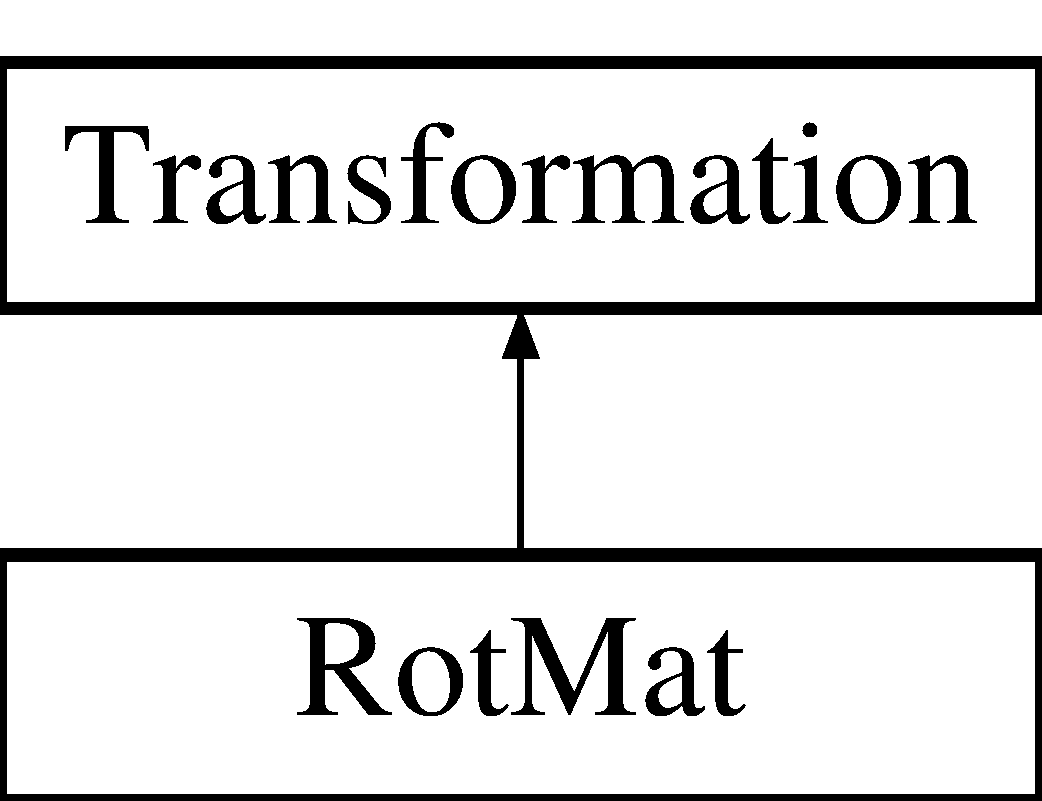
\includegraphics[height=2.000000cm]{class_rot_mat}
\end{center}
\end{figure}
\subsection*{Public Member Functions}
\begin{DoxyCompactItemize}
\item 
\hypertarget{class_rot_mat_abe1e5d870c095d4345d58d5539a3f86a}{const \hyperlink{class_rot_mat}{Rot\-Mat} \& {\bfseries Reset} (const \hyperlink{class_angel_1_1mat4}{Angel\-::mat4} \&New\-State)}\label{class_rot_mat_abe1e5d870c095d4345d58d5539a3f86a}

\item 
\hypertarget{class_rot_mat_ad4def0c34e58da1bd9b3a39f6a9fce91}{const \hyperlink{class_rot_mat}{Rot\-Mat} \& {\bfseries Rotate\-X} (const G\-Lfloat theta, bool postmult=true)}\label{class_rot_mat_ad4def0c34e58da1bd9b3a39f6a9fce91}

\item 
\hypertarget{class_rot_mat_a6823dc0196574a21bddfd166024204f5}{const \hyperlink{class_rot_mat}{Rot\-Mat} \& {\bfseries Rotate\-Y} (const G\-Lfloat theta, bool postmult=true)}\label{class_rot_mat_a6823dc0196574a21bddfd166024204f5}

\item 
\hypertarget{class_rot_mat_a8f93106da83a30fb56482859a39ed2a4}{const \hyperlink{class_rot_mat}{Rot\-Mat} \& {\bfseries Rotate\-Z} (const G\-Lfloat theta, bool postmult=true)}\label{class_rot_mat_a8f93106da83a30fb56482859a39ed2a4}

\item 
\hypertarget{class_rot_mat_af5ba2e61406934af90e612a037659fb0}{const \hyperlink{class_rot_mat}{Rot\-Mat} \& {\bfseries Adjust} (const \hyperlink{class_angel_1_1mat4}{Angel\-::mat4} \&Adjustment, bool postmult=true)}\label{class_rot_mat_af5ba2e61406934af90e612a037659fb0}

\item 
\hypertarget{class_transformation_ae6a57a1ee74ca1da1b8aef3d328a8772}{const \hyperlink{class_angel_1_1mat4}{Angel\-::mat4} \& {\bfseries Matrix} (void) const }\label{class_transformation_ae6a57a1ee74ca1da1b8aef3d328a8772}

\item 
\hypertarget{class_transformation_afdfbf48815a5b0d885f3b93f04cd2c66}{\hyperlink{class_angel_1_1mat4}{Angel\-::mat4} {\bfseries operator$\ast$} (const \hyperlink{class_angel_1_1mat4}{Angel\-::mat4} \&rhs) const }\label{class_transformation_afdfbf48815a5b0d885f3b93f04cd2c66}

\item 
\hypertarget{class_transformation_a85b923e0066365ef2e4aec3671396410}{\hyperlink{class_angel_1_1mat4}{Angel\-::mat4} {\bfseries operator$\ast$} (const \hyperlink{class_transformation}{Transformation} \&rhs) const }\label{class_transformation_a85b923e0066365ef2e4aec3671396410}

\end{DoxyCompactItemize}
\subsection*{Protected Attributes}
\begin{DoxyCompactItemize}
\item 
\hypertarget{class_transformation_a5f39fb578a1cdf78ca85efbd932d3834}{\hyperlink{class_angel_1_1mat4}{Angel\-::mat4} {\bfseries mat}}\label{class_transformation_a5f39fb578a1cdf78ca85efbd932d3834}

\end{DoxyCompactItemize}


\subsection{Detailed Description}
Rotations. 

Definition at line 33 of file Transformation.\-hpp.



The documentation for this class was generated from the following files\-:\begin{DoxyCompactItemize}
\item 
Transformation.\-hpp\item 
Transformation.\-cpp\end{DoxyCompactItemize}

\hypertarget{class_scale_mat}{\section{Scale\-Mat Class Reference}
\label{class_scale_mat}\index{Scale\-Mat@{Scale\-Mat}}
}
Inheritance diagram for Scale\-Mat\-:\begin{figure}[H]
\begin{center}
\leavevmode
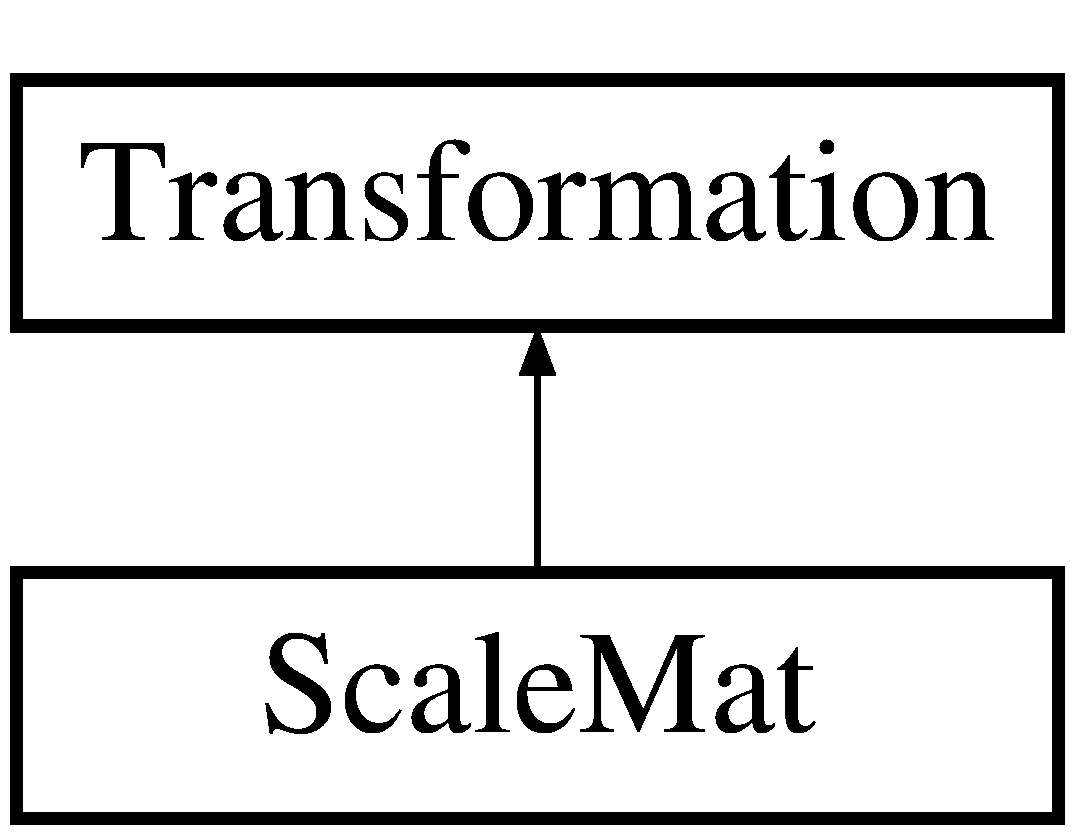
\includegraphics[height=2.000000cm]{class_scale_mat}
\end{center}
\end{figure}
\subsection*{Public Member Functions}
\begin{DoxyCompactItemize}
\item 
\hypertarget{class_scale_mat_aa72e3e61eddd0e88092e6cc76cc78972}{const \hyperlink{class_scale_mat}{Scale\-Mat} \& {\bfseries Set} (const float x, const float y, const float z)}\label{class_scale_mat_aa72e3e61eddd0e88092e6cc76cc78972}

\item 
\hypertarget{class_scale_mat_aea523b732204366c105809fc447ff07e}{const \hyperlink{class_scale_mat}{Scale\-Mat} \& {\bfseries Set} (const float pct)}\label{class_scale_mat_aea523b732204366c105809fc447ff07e}

\item 
\hypertarget{class_scale_mat_ad259370ba433114d9cdbd9d817552905}{const \hyperlink{class_scale_mat}{Scale\-Mat} \& {\bfseries Adjust} (const float x, const float y, const float z)}\label{class_scale_mat_ad259370ba433114d9cdbd9d817552905}

\item 
\hypertarget{class_scale_mat_af915563091d994e41c309a2bcd31615e}{const \hyperlink{class_scale_mat}{Scale\-Mat} \& {\bfseries Adjust} (const float pct)}\label{class_scale_mat_af915563091d994e41c309a2bcd31615e}

\item 
\hypertarget{class_transformation_ae6a57a1ee74ca1da1b8aef3d328a8772}{const \hyperlink{class_angel_1_1mat4}{Angel\-::mat4} \& {\bfseries Matrix} (void) const }\label{class_transformation_ae6a57a1ee74ca1da1b8aef3d328a8772}

\item 
\hypertarget{class_transformation_afdfbf48815a5b0d885f3b93f04cd2c66}{\hyperlink{class_angel_1_1mat4}{Angel\-::mat4} {\bfseries operator$\ast$} (const \hyperlink{class_angel_1_1mat4}{Angel\-::mat4} \&rhs) const }\label{class_transformation_afdfbf48815a5b0d885f3b93f04cd2c66}

\item 
\hypertarget{class_transformation_a85b923e0066365ef2e4aec3671396410}{\hyperlink{class_angel_1_1mat4}{Angel\-::mat4} {\bfseries operator$\ast$} (const \hyperlink{class_transformation}{Transformation} \&rhs) const }\label{class_transformation_a85b923e0066365ef2e4aec3671396410}

\end{DoxyCompactItemize}
\subsection*{Protected Attributes}
\begin{DoxyCompactItemize}
\item 
\hypertarget{class_transformation_a5f39fb578a1cdf78ca85efbd932d3834}{\hyperlink{class_angel_1_1mat4}{Angel\-::mat4} {\bfseries mat}}\label{class_transformation_a5f39fb578a1cdf78ca85efbd932d3834}

\end{DoxyCompactItemize}


\subsection{Detailed Description}


Definition at line 63 of file Transformation.\-hpp.



The documentation for this class was generated from the following files\-:\begin{DoxyCompactItemize}
\item 
Transformation.\-hpp\item 
Transformation.\-cpp\end{DoxyCompactItemize}

\hypertarget{class_scene}{\section{Scene Class Reference}
\label{class_scene}\index{Scene@{Scene}}
}
Inheritance diagram for Scene\-:\begin{figure}[H]
\begin{center}
\leavevmode
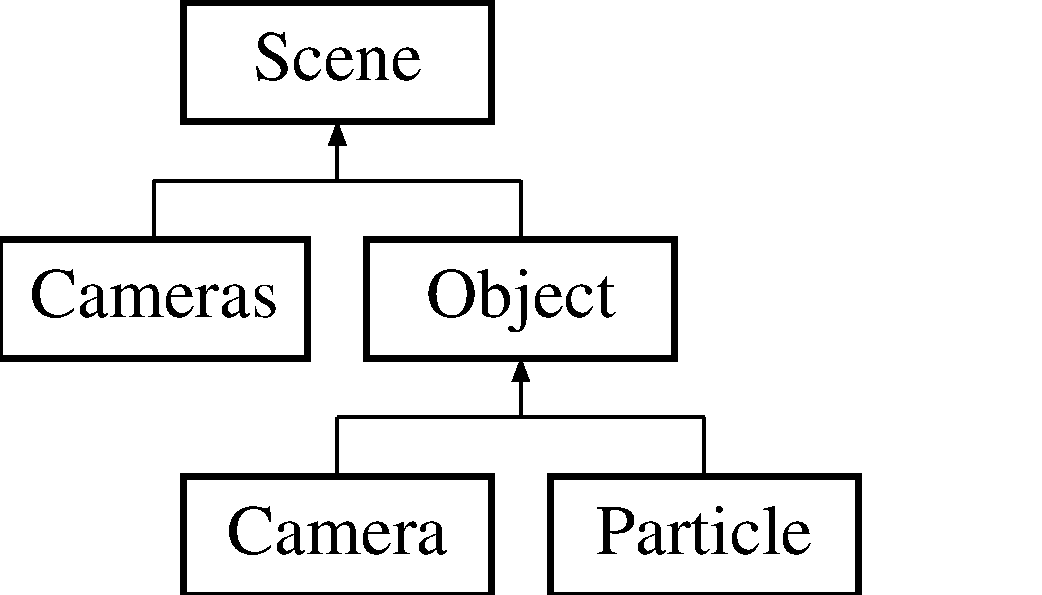
\includegraphics[height=3.000000cm]{class_scene}
\end{center}
\end{figure}
\subsection*{Public Member Functions}
\begin{DoxyCompactItemize}
\item 
virtual void \hyperlink{class_scene_a7137a7302c21ac4dd44e746bfb6f7cf8}{Shader} (G\-Luint g\-Shader)
\begin{DoxyCompactList}\small\item\em Sets the Default shader for the scene. \end{DoxyCompactList}\item 
G\-Luint \hyperlink{class_scene_af1e8ba8802f3bf83cebbfcbf3ed7c333}{Shader} (void)
\begin{DoxyCompactList}\small\item\em Retrieves the handle for the default shader for the scene. \end{DoxyCompactList}\item 
\hypertarget{class_scene_a366b5dec1ecf66a887b4d0dedcd1aa3b}{\hyperlink{class_object}{Object} $\ast$ {\bfseries Add\-Object} (const std\-::string \&obj\-Name, G\-Luint Object\-\_\-\-Shader=0)}\label{class_scene_a366b5dec1ecf66a887b4d0dedcd1aa3b}

\item 
\hypertarget{class_scene_a3bd9fa1058f506c04162b9283e97d20e}{void {\bfseries Del\-Object} (const std\-::string \&obj\-Name)}\label{class_scene_a3bd9fa1058f506c04162b9283e97d20e}

\item 
\hypertarget{class_scene_a43fd3c56db5dc940d1724b9573c9a360}{void {\bfseries Del\-Object} (void)}\label{class_scene_a43fd3c56db5dc940d1724b9573c9a360}

\item 
\hypertarget{class_scene_abdfd15e7987aa261840d5ecc265170df}{void {\bfseries Pop\-Object} (void)}\label{class_scene_abdfd15e7987aa261840d5ecc265170df}

\item 
\hypertarget{class_scene_a82759ded1f6f87a91b8d10ed87501958}{void \hyperlink{class_scene_a82759ded1f6f87a91b8d10ed87501958}{Destroy\-Object} (void)}\label{class_scene_a82759ded1f6f87a91b8d10ed87501958}

\begin{DoxyCompactList}\small\item\em Completely remove this object and all his children. \end{DoxyCompactList}\item 
\hypertarget{class_scene_a70fcdad192a4c6ff508125de8af6cf4d}{\hyperlink{class_object}{Object} $\ast$ {\bfseries next} (void)}\label{class_scene_a70fcdad192a4c6ff508125de8af6cf4d}

\item 
\hypertarget{class_scene_ac852d5d763eb35b4908c9aa7ea54d1ae}{\hyperlink{class_object}{Object} $\ast$ {\bfseries prev} (void)}\label{class_scene_ac852d5d763eb35b4908c9aa7ea54d1ae}

\item 
\hypertarget{class_scene_ad0ea1a6bcf7815c63988bd937f06eb23}{\hyperlink{class_object}{Object} $\ast$ {\bfseries active} (void) const }\label{class_scene_ad0ea1a6bcf7815c63988bd937f06eb23}

\item 
\hypertarget{class_scene_ad5a91c929b569b9111061eec16b3febf}{void {\bfseries Draw} (void)}\label{class_scene_ad5a91c929b569b9111061eec16b3febf}

\item 
\hypertarget{class_scene_ae9b69d8db8a46991017635f22e45baad}{\hyperlink{class_object}{Object} $\ast$ {\bfseries operator\mbox{[}$\,$\mbox{]}} (const std\-::string \&objname)}\label{class_scene_ae9b69d8db8a46991017635f22e45baad}

\item 
\hypertarget{class_scene_aa6e6354478dc7df82446b3abf9f91d96}{{\bfseries Scene} (const \hyperlink{class_scene}{Scene} \&copy)}\label{class_scene_aa6e6354478dc7df82446b3abf9f91d96}

\item 
\hypertarget{class_scene_a6336263b33b06ce4ace53599ffd8122c}{\hyperlink{class_scene}{Scene} \& {\bfseries operator=} (const \hyperlink{class_scene}{Scene} \&copy)}\label{class_scene_a6336263b33b06ce4ace53599ffd8122c}

\end{DoxyCompactItemize}
\subsection*{Protected Member Functions}
\begin{DoxyCompactItemize}
\item 
void \hyperlink{class_scene_a8bbe0e5b1bfc71034b18e240e86aa285}{Delete\-Object} (\hyperlink{class_object}{Object} $\ast$obj)
\begin{DoxyCompactList}\small\item\em Delete\-Object is the actual implementation function that will remove an \hyperlink{class_object}{Object} from the \hyperlink{class_scene}{Scene} list and \hyperlink{class_scene}{Scene} map, then free the object. \end{DoxyCompactList}\item 
\hypertarget{class_scene_ae8d51ddc196248a7cbd1f3640851dbd4}{void {\bfseries Insert\-Object} (const std\-::string name, \hyperlink{class_object}{Object} $\ast$obj)}\label{class_scene_ae8d51ddc196248a7cbd1f3640851dbd4}

\end{DoxyCompactItemize}
\subsection*{Protected Attributes}
\begin{DoxyCompactItemize}
\item 
\hypertarget{class_scene_acdd0123ca6b2d64d8d447bb485b235fc}{std\-::list$<$ \hyperlink{class_object}{Object} $\ast$ $>$ {\bfseries \-\_\-list}}\label{class_scene_acdd0123ca6b2d64d8d447bb485b235fc}

\item 
\hypertarget{class_scene_a8bd5d86484a12255b26b92b6cbf8d29a}{std\-::map$<$ std\-::string, \hyperlink{class_object}{Object} $\ast$ $>$ {\bfseries \-\_\-map}}\label{class_scene_a8bd5d86484a12255b26b92b6cbf8d29a}

\item 
\hypertarget{class_scene_ae87ca5350fcc595f3f15a4fd3c39f3d9}{std\-::list$<$ \hyperlink{class_object}{Object} $\ast$ $>$\-::iterator {\bfseries \-\_\-current\-Obj}}\label{class_scene_ae87ca5350fcc595f3f15a4fd3c39f3d9}

\item 
\hypertarget{class_scene_a8f9bdd8ec5edb1f414fbd314a36e2724}{G\-Luint {\bfseries \-\_\-g\-Shader}}\label{class_scene_a8f9bdd8ec5edb1f414fbd314a36e2724}

\end{DoxyCompactItemize}


\subsection{Detailed Description}


Definition at line 12 of file Scene.\-hpp.



\subsection{Member Function Documentation}
\hypertarget{class_scene_a8bbe0e5b1bfc71034b18e240e86aa285}{\index{Scene@{Scene}!Delete\-Object@{Delete\-Object}}
\index{Delete\-Object@{Delete\-Object}!Scene@{Scene}}
\subsubsection[{Delete\-Object}]{\setlength{\rightskip}{0pt plus 5cm}void Scene\-::\-Delete\-Object (
\begin{DoxyParamCaption}
\item[{{\bf Object} $\ast$}]{obj}
\end{DoxyParamCaption}
)\hspace{0.3cm}{\ttfamily [protected]}}}\label{class_scene_a8bbe0e5b1bfc71034b18e240e86aa285}


Delete\-Object is the actual implementation function that will remove an \hyperlink{class_object}{Object} from the \hyperlink{class_scene}{Scene} list and \hyperlink{class_scene}{Scene} map, then free the object. 


\begin{DoxyParams}{Parameters}
{\em obj} & The pointer to the object to free. \\
\hline
\end{DoxyParams}


Definition at line 76 of file Scene.\-cpp.

\hypertarget{class_scene_a7137a7302c21ac4dd44e746bfb6f7cf8}{\index{Scene@{Scene}!Shader@{Shader}}
\index{Shader@{Shader}!Scene@{Scene}}
\subsubsection[{Shader}]{\setlength{\rightskip}{0pt plus 5cm}void Scene\-::\-Shader (
\begin{DoxyParamCaption}
\item[{G\-Luint}]{g\-Shader}
\end{DoxyParamCaption}
)\hspace{0.3cm}{\ttfamily [virtual]}}}\label{class_scene_a7137a7302c21ac4dd44e746bfb6f7cf8}


Sets the Default shader for the scene. 

In the context of inheritance by objects, This sets the shader to use to render the physical object.


\begin{DoxyParams}{Parameters}
{\em g\-Shader} & The G\-Luint handle to the shader to use.\\
\hline
\end{DoxyParams}
\begin{DoxyReturn}{Returns}
void. 
\end{DoxyReturn}


Reimplemented in \hyperlink{class_object_aa52c30bca96800cecba55f446e147859}{Object}.



Definition at line 54 of file Scene.\-cpp.

\hypertarget{class_scene_af1e8ba8802f3bf83cebbfcbf3ed7c333}{\index{Scene@{Scene}!Shader@{Shader}}
\index{Shader@{Shader}!Scene@{Scene}}
\subsubsection[{Shader}]{\setlength{\rightskip}{0pt plus 5cm}G\-Luint Scene\-::\-Shader (
\begin{DoxyParamCaption}
\item[{void}]{}
\end{DoxyParamCaption}
)}}\label{class_scene_af1e8ba8802f3bf83cebbfcbf3ed7c333}


Retrieves the handle for the default shader for the scene. 

In the context of inheritance by objects, This retrieves the shader handle to use to draw the object.

\begin{DoxyReturn}{Returns}
A G\-Luint handle to the shader program. 
\end{DoxyReturn}


Definition at line 66 of file Scene.\-cpp.



The documentation for this class was generated from the following files\-:\begin{DoxyCompactItemize}
\item 
Scene.\-hpp\item 
Scene.\-cpp\end{DoxyCompactItemize}

\hypertarget{class_screen}{\section{Screen Class Reference}
\label{class_screen}\index{Screen@{Screen}}
}
\subsection*{Public Member Functions}
\begin{DoxyCompactItemize}
\item 
\hypertarget{class_screen_ad97151af2e654778bad86043c32fe19f}{{\bfseries Screen} (int x=0, int y=0)}\label{class_screen_ad97151af2e654778bad86043c32fe19f}

\item 
\hypertarget{class_screen_a7b45282430392ffa8b5891936363f8f8}{{\bfseries Screen} (const \hyperlink{struct_angel_1_1vec2}{vec2} \&new\-Size)}\label{class_screen_a7b45282430392ffa8b5891936363f8f8}

\item 
\hypertarget{class_screen_a478c5176fd4fdc8af48f2bd7e824329d}{void {\bfseries Size} (int x, int y)}\label{class_screen_a478c5176fd4fdc8af48f2bd7e824329d}

\item 
\hypertarget{class_screen_a5fa4071af08df619e7cb4311bc0efb45}{void {\bfseries Size} (const \hyperlink{struct_angel_1_1vec2}{vec2} \&new\-Size)}\label{class_screen_a5fa4071af08df619e7cb4311bc0efb45}

\item 
\hypertarget{class_screen_a6f22423a037d9cf406d3ca4dd79b94b5}{const \hyperlink{struct_angel_1_1vec2}{vec2} \& {\bfseries Size} (void)}\label{class_screen_a6f22423a037d9cf406d3ca4dd79b94b5}

\item 
\hypertarget{class_screen_aa9a4a2e113af54d7164463bef8e78471}{int {\bfseries Width} (void)}\label{class_screen_aa9a4a2e113af54d7164463bef8e78471}

\item 
\hypertarget{class_screen_ad532ef57bbdb9a1e1540812a02eece23}{int {\bfseries Height} (void)}\label{class_screen_ad532ef57bbdb9a1e1540812a02eece23}

\item 
\hypertarget{class_screen_a00be376c569ac4b71d770f34e297f332}{const \hyperlink{struct_angel_1_1vec2}{vec2} \& {\bfseries Center} (void)}\label{class_screen_a00be376c569ac4b71d770f34e297f332}

\item 
\hypertarget{class_screen_a434f489a1b9d40319f7f6dbbf11db456}{int {\bfseries Midpoint\-X} (void)}\label{class_screen_a434f489a1b9d40319f7f6dbbf11db456}

\item 
\hypertarget{class_screen_a7b574e8ded50718dc1523180102e2f41}{int {\bfseries Midpoint\-Y} (void)}\label{class_screen_a7b574e8ded50718dc1523180102e2f41}

\end{DoxyCompactItemize}
\subsection*{Public Attributes}
\begin{DoxyCompactItemize}
\item 
\hypertarget{class_screen_a0098c32ec26cba2df8108d7b706986e5}{\hyperlink{class_cameras}{Cameras} {\bfseries \-\_\-cam\-List}}\label{class_screen_a0098c32ec26cba2df8108d7b706986e5}

\end{DoxyCompactItemize}
\subsection*{Private Attributes}
\begin{DoxyCompactItemize}
\item 
\hypertarget{class_screen_a02a1812a3807a9c4db6d4456861a7130}{\hyperlink{struct_angel_1_1vec2}{vec2} {\bfseries \-\_\-size}}\label{class_screen_a02a1812a3807a9c4db6d4456861a7130}

\item 
\hypertarget{class_screen_a1c82610b27dd93ae998b96d1fe11c792}{\hyperlink{struct_angel_1_1vec2}{vec2} {\bfseries \-\_\-center}}\label{class_screen_a1c82610b27dd93ae998b96d1fe11c792}

\end{DoxyCompactItemize}


\subsection{Detailed Description}


Definition at line 8 of file Screen.\-hpp.



The documentation for this class was generated from the following files\-:\begin{DoxyCompactItemize}
\item 
Screen.\-hpp\item 
Screen.\-cpp\end{DoxyCompactItemize}

\hypertarget{class_spelchk_camera}{\section{Spelchk\-Camera Class Reference}
\label{class_spelchk_camera}\index{Spelchk\-Camera@{Spelchk\-Camera}}
}
\subsection*{Public Member Functions}
\begin{DoxyCompactItemize}
\item 
\hypertarget{class_spelchk_camera_a1d894472ef9e588ddeb56434e549cd0a}{{\bfseries Spelchk\-Camera} (\hyperlink{struct_angel_1_1vec4}{vec4} initial\-Translation\-Vector)}\label{class_spelchk_camera_a1d894472ef9e588ddeb56434e549cd0a}

\item 
\hypertarget{class_spelchk_camera_a2a9aa83f6e5d3d2371dd00ae162aef30}{\hyperlink{class_angel_1_1mat4}{mat4} {\bfseries get\-Projection\-Matrix} ()}\label{class_spelchk_camera_a2a9aa83f6e5d3d2371dd00ae162aef30}

\item 
\hypertarget{class_spelchk_camera_af702dfbd3c3719e4b738440bb2269922}{\hyperlink{class_angel_1_1mat4}{mat4} {\bfseries get\-Model\-View\-Matrix} ()}\label{class_spelchk_camera_af702dfbd3c3719e4b738440bb2269922}

\item 
\hypertarget{class_spelchk_camera_a4ad8fbfe69914453580c02406bffc501}{\hyperlink{struct_angel_1_1vec4}{vec4} {\bfseries get\-Translation\-Vector} ()}\label{class_spelchk_camera_a4ad8fbfe69914453580c02406bffc501}

\item 
\hypertarget{class_spelchk_camera_a1396d6aa2a3e85d9ed8b90c17751da41}{void {\bfseries move\-Camera} (float x\-Depth, float y\-Depth, float z\-Depth)}\label{class_spelchk_camera_a1396d6aa2a3e85d9ed8b90c17751da41}

\item 
\hypertarget{class_spelchk_camera_aa012e2d10f196ae007a8f8b4ac8471c3}{void {\bfseries rotate\-Camera} (float x\-Angle, float y\-Angle, float z\-Angle)}\label{class_spelchk_camera_aa012e2d10f196ae007a8f8b4ac8471c3}

\item 
\hypertarget{class_spelchk_camera_a24f5fe7d296bcd7ec9d70b25b6a92fe5}{void {\bfseries set\-Screen\-Size} (int width, int height)}\label{class_spelchk_camera_a24f5fe7d296bcd7ec9d70b25b6a92fe5}

\item 
\hypertarget{class_spelchk_camera_a95b87c80007941d85d26c43d30fa7f87}{void {\bfseries set\-Projection} (int projection\-Type)}\label{class_spelchk_camera_a95b87c80007941d85d26c43d30fa7f87}

\item 
\hypertarget{class_spelchk_camera_a29d4ba987d9f3e1c47e1103fcea0ae2b}{void {\bfseries reset} ()}\label{class_spelchk_camera_a29d4ba987d9f3e1c47e1103fcea0ae2b}

\item 
\hypertarget{class_spelchk_camera_a20436fee96b0d6a1279d10b88e20f520}{void {\bfseries set\-Light\-Movement\-Ref} (G\-Luint ref)}\label{class_spelchk_camera_a20436fee96b0d6a1279d10b88e20f520}

\item 
\hypertarget{class_spelchk_camera_aed5d76d2de23473dec034161efe29275}{void {\bfseries set\-Light\-Movement\-Time} (float elapsed)}\label{class_spelchk_camera_aed5d76d2de23473dec034161efe29275}

\item 
\hypertarget{class_spelchk_camera_a90aa5e06ba61d44e63535acf2cc3e373}{void {\bfseries get\-Ready\-For\-Zero} (int usernum)}\label{class_spelchk_camera_a90aa5e06ba61d44e63535acf2cc3e373}

\item 
\hypertarget{class_spelchk_camera_afc39db6b4eab85070aa5d7494d0c5198}{void {\bfseries head\-Movement} (int usernum, double x, double y, double z)}\label{class_spelchk_camera_afc39db6b4eab85070aa5d7494d0c5198}

\end{DoxyCompactItemize}
\subsection*{Private Member Functions}
\begin{DoxyCompactItemize}
\item 
\hypertarget{class_spelchk_camera_a539230ff6d91932526666d4eee9d6c0d}{void {\bfseries calculate\-Translation\-Vector} ()}\label{class_spelchk_camera_a539230ff6d91932526666d4eee9d6c0d}

\end{DoxyCompactItemize}
\subsection*{Private Attributes}
\begin{DoxyCompactItemize}
\item 
\hypertarget{class_spelchk_camera_a56626b721de172eed34cd008db1e3cfe}{int {\bfseries projection\-Type}}\label{class_spelchk_camera_a56626b721de172eed34cd008db1e3cfe}

\item 
\hypertarget{class_spelchk_camera_a7100656d4105997c30736993767a31f9}{G\-Lfloat {\bfseries fovy}}\label{class_spelchk_camera_a7100656d4105997c30736993767a31f9}

\item 
\hypertarget{class_spelchk_camera_a70d9a9d5f6176a0c9d26bd645536085c}{G\-Lfloat {\bfseries aspect}}\label{class_spelchk_camera_a70d9a9d5f6176a0c9d26bd645536085c}

\item 
\hypertarget{class_spelchk_camera_ae8f0c6ccfef8af60b4e4b7178ed79ddd}{G\-Lfloat {\bfseries left}}\label{class_spelchk_camera_ae8f0c6ccfef8af60b4e4b7178ed79ddd}

\item 
\hypertarget{class_spelchk_camera_a7c0c8e4ef77ab6235b764099c4178ac9}{G\-Lfloat {\bfseries right}}\label{class_spelchk_camera_a7c0c8e4ef77ab6235b764099c4178ac9}

\item 
\hypertarget{class_spelchk_camera_ac63e0cb41beb7ba21b4a93411057fb11}{G\-Lfloat {\bfseries bottom}}\label{class_spelchk_camera_ac63e0cb41beb7ba21b4a93411057fb11}

\item 
\hypertarget{class_spelchk_camera_a91da81606e111b5346b9ff01b8ee51e4}{G\-Lfloat {\bfseries top}}\label{class_spelchk_camera_a91da81606e111b5346b9ff01b8ee51e4}

\item 
\hypertarget{class_spelchk_camera_a5ff79a52200bff0010dec68f6f2fc81f}{G\-Lfloat {\bfseries z\-Near}}\label{class_spelchk_camera_a5ff79a52200bff0010dec68f6f2fc81f}

\item 
\hypertarget{class_spelchk_camera_a5e346a9b0f4513cd73e8c662d9b68ce8}{G\-Lfloat {\bfseries z\-Far}}\label{class_spelchk_camera_a5e346a9b0f4513cd73e8c662d9b68ce8}

\item 
\hypertarget{class_spelchk_camera_a95814c7cdb0c22f786c550f0be15d861}{G\-Luint {\bfseries time\-Ref}}\label{class_spelchk_camera_a95814c7cdb0c22f786c550f0be15d861}

\item 
\hypertarget{class_spelchk_camera_a151379f37af88e08c6d8cb8e68c803f5}{int {\bfseries screen\-Width}}\label{class_spelchk_camera_a151379f37af88e08c6d8cb8e68c803f5}

\item 
\hypertarget{class_spelchk_camera_ac8c840647d7f35bb118b289793ff5454}{int {\bfseries screen\-Height}}\label{class_spelchk_camera_ac8c840647d7f35bb118b289793ff5454}

\item 
\hypertarget{class_spelchk_camera_a36003c28aa94824059381841d4f0081f}{G\-Lfloat {\bfseries x\-Depth}}\label{class_spelchk_camera_a36003c28aa94824059381841d4f0081f}

\item 
\hypertarget{class_spelchk_camera_a47c24171c6228b32362160990725f52e}{G\-Lfloat {\bfseries y\-Depth}}\label{class_spelchk_camera_a47c24171c6228b32362160990725f52e}

\item 
\hypertarget{class_spelchk_camera_ad70aebd6b7292aa9ad917e1bc264b5bd}{G\-Lfloat {\bfseries z\-Depth}}\label{class_spelchk_camera_ad70aebd6b7292aa9ad917e1bc264b5bd}

\item 
\hypertarget{class_spelchk_camera_a96902d7291fd719ae0d5630fc1966cab}{G\-Lfloat {\bfseries x\-Angle}}\label{class_spelchk_camera_a96902d7291fd719ae0d5630fc1966cab}

\item 
\hypertarget{class_spelchk_camera_a1a2a01ff4bf6ed7e0aea35baf64c52d3}{G\-Lfloat {\bfseries y\-Angle}}\label{class_spelchk_camera_a1a2a01ff4bf6ed7e0aea35baf64c52d3}

\item 
\hypertarget{class_spelchk_camera_a22de39eb2216ae32f2aefbdd06d26670}{G\-Lfloat {\bfseries z\-Angle}}\label{class_spelchk_camera_a22de39eb2216ae32f2aefbdd06d26670}

\item 
\hypertarget{class_spelchk_camera_ad681727f16e8864332beb03a8d56f38c}{G\-Lfloat {\bfseries x\-Head}}\label{class_spelchk_camera_ad681727f16e8864332beb03a8d56f38c}

\item 
\hypertarget{class_spelchk_camera_aab34b46f554bd49958e22deb1dfcdfc1}{G\-Lfloat {\bfseries y\-Head}}\label{class_spelchk_camera_aab34b46f554bd49958e22deb1dfcdfc1}

\item 
\hypertarget{class_spelchk_camera_a900decac3d9387e3a90f9a363f171241}{G\-Lfloat {\bfseries z\-Head}}\label{class_spelchk_camera_a900decac3d9387e3a90f9a363f171241}

\item 
\hypertarget{class_spelchk_camera_a96a0eaa30df58f418b62dd32a87aacdd}{float {\bfseries x\-Head\-Start}}\label{class_spelchk_camera_a96a0eaa30df58f418b62dd32a87aacdd}

\item 
\hypertarget{class_spelchk_camera_a6160bf79c12028d38e3a722f47b73689}{float {\bfseries y\-Head\-Start}}\label{class_spelchk_camera_a6160bf79c12028d38e3a722f47b73689}

\item 
\hypertarget{class_spelchk_camera_a2d4ff9d44d319beae940893c13cd6d23}{float {\bfseries z\-Head\-Start}}\label{class_spelchk_camera_a2d4ff9d44d319beae940893c13cd6d23}

\item 
\hypertarget{class_spelchk_camera_a4e29677cebaa80d8559eaa5b97f67a9d}{G\-Lfloat {\bfseries x\-Head\-Angle}}\label{class_spelchk_camera_a4e29677cebaa80d8559eaa5b97f67a9d}

\item 
\hypertarget{class_spelchk_camera_a6cbc7eb6281d9b5d3e52f9cc368e099e}{G\-Lfloat {\bfseries y\-Head\-Angle}}\label{class_spelchk_camera_a6cbc7eb6281d9b5d3e52f9cc368e099e}

\item 
\hypertarget{class_spelchk_camera_adadeec344d21294df061f66f184c0dda}{G\-Lfloat {\bfseries z\-Head\-Angle}}\label{class_spelchk_camera_adadeec344d21294df061f66f184c0dda}

\item 
\hypertarget{class_spelchk_camera_afc4abd0c3662dc3808cb073650547d36}{\hyperlink{struct_angel_1_1vec4}{vec4} {\bfseries initial\-Translation\-Vector}}\label{class_spelchk_camera_afc4abd0c3662dc3808cb073650547d36}

\item 
\hypertarget{class_spelchk_camera_aef04e503f7376447684b6594a9cd79eb}{\hyperlink{struct_angel_1_1vec4}{vec4} {\bfseries translation\-Vector}}\label{class_spelchk_camera_aef04e503f7376447684b6594a9cd79eb}

\item 
\hypertarget{class_spelchk_camera_a30c3cde28c3d5c137b784e15d58233c4}{\hyperlink{struct_angel_1_1vec4}{vec4} {\bfseries old\-Translation\-Vector}}\label{class_spelchk_camera_a30c3cde28c3d5c137b784e15d58233c4}

\item 
\hypertarget{class_spelchk_camera_a733c3b94be2ec8b25c69f124fba72294}{\hyperlink{class_angel_1_1mat4}{mat4} {\bfseries model\-View\-Matrix}}\label{class_spelchk_camera_a733c3b94be2ec8b25c69f124fba72294}

\item 
\hypertarget{class_spelchk_camera_abf7dde00eb7354162a80b4675b0b1b96}{int {\bfseries inbound\-Head\-Data}}\label{class_spelchk_camera_abf7dde00eb7354162a80b4675b0b1b96}

\item 
\hypertarget{class_spelchk_camera_afa0999e81fc3478d2791fd7febc845bf}{\hyperlink{struct_angel_1_1vec4}{vec4} {\bfseries initial\-Head\-Position}}\label{class_spelchk_camera_afa0999e81fc3478d2791fd7febc845bf}

\end{DoxyCompactItemize}


\subsection{Detailed Description}


Definition at line 16 of file Spelchk\-Camera.\-hpp.



The documentation for this class was generated from the following files\-:\begin{DoxyCompactItemize}
\item 
Spelchk\-Camera.\-hpp\item 
Spelchk\-Camera.\-cpp\end{DoxyCompactItemize}

\hypertarget{class_timer}{\section{Timer Class Reference}
\label{class_timer}\index{Timer@{Timer}}
}
\subsection*{Public Member Functions}
\begin{DoxyCompactItemize}
\item 
unsigned long \hyperlink{class_timer_a4e69d3c5a312d1b29d1735b2c5bccefb}{Tick} ()
\begin{DoxyCompactList}\small\item\em Tick is an alias for Tock. \end{DoxyCompactList}\item 
unsigned long \hyperlink{class_timer_a2c58a2e04e1e30926805aa4e82d2a0a5}{Tock} ()
\begin{DoxyCompactList}\small\item\em Tock returns the time elapsed since the last Tock. \end{DoxyCompactList}\item 
unsigned long \hyperlink{class_timer_a4f68da5b62cb1d1b2dd0c8549eb6286d}{Delta} () const 
\begin{DoxyCompactList}\small\item\em Delta returns the time elapsed between the last Tick and the last Tock. \end{DoxyCompactList}\item 
double \hyperlink{class_timer_a25ed035b0da5b177050c922660acf864}{Scale} () const 
\begin{DoxyCompactList}\small\item\em Scale returns the relative lateness or eagerness of the \hyperlink{class_timer}{Timer}, Relative to a benchmark or Key Frame Rate (The default is 60\-F\-P\-S, or 16667 msec.) \end{DoxyCompactList}\end{DoxyCompactItemize}
\subsection*{Private Attributes}
\begin{DoxyCompactItemize}
\item 
\hypertarget{class_timer_a384a34d671fa58160f0ea13713645462}{struct timeval {\bfseries \-\_\-\-T1}}\label{class_timer_a384a34d671fa58160f0ea13713645462}

\item 
\hypertarget{class_timer_a22691ac7f27eed709461091c1125d931}{struct timeval {\bfseries \-\_\-\-T2}}\label{class_timer_a22691ac7f27eed709461091c1125d931}

\item 
\hypertarget{class_timer_a2a80ef1463e87f63e6ccc45a3fbe5ac2}{unsigned long {\bfseries \-\_\-delta}}\label{class_timer_a2a80ef1463e87f63e6ccc45a3fbe5ac2}

\item 
\hypertarget{class_timer_a02c5ec526c6bad4f0f2352325b4ac4f3}{double {\bfseries \-\_\-scale}}\label{class_timer_a02c5ec526c6bad4f0f2352325b4ac4f3}

\end{DoxyCompactItemize}


\subsection{Detailed Description}


Definition at line 6 of file Timer.\-hpp.



\subsection{Member Function Documentation}
\hypertarget{class_timer_a4f68da5b62cb1d1b2dd0c8549eb6286d}{\index{Timer@{Timer}!Delta@{Delta}}
\index{Delta@{Delta}!Timer@{Timer}}
\subsubsection[{Delta}]{\setlength{\rightskip}{0pt plus 5cm}unsigned long Timer\-::\-Delta (
\begin{DoxyParamCaption}
\item[{void}]{}
\end{DoxyParamCaption}
) const}}\label{class_timer_a4f68da5b62cb1d1b2dd0c8549eb6286d}


Delta returns the time elapsed between the last Tick and the last Tock. 

Does not start a new timer. \begin{DoxyReturn}{Returns}
Time elapsed in Microseconds, or Nanoseconds if \-\_\-\-R\-T was enabled. 
\end{DoxyReturn}


Definition at line 59 of file Timer.\-cpp.

\hypertarget{class_timer_a25ed035b0da5b177050c922660acf864}{\index{Timer@{Timer}!Scale@{Scale}}
\index{Scale@{Scale}!Timer@{Timer}}
\subsubsection[{Scale}]{\setlength{\rightskip}{0pt plus 5cm}double Timer\-::\-Scale (
\begin{DoxyParamCaption}
\item[{void}]{}
\end{DoxyParamCaption}
) const}}\label{class_timer_a25ed035b0da5b177050c922660acf864}


Scale returns the relative lateness or eagerness of the \hyperlink{class_timer}{Timer}, Relative to a benchmark or Key Frame Rate (The default is 60\-F\-P\-S, or 16667 msec.) 

\begin{DoxyReturn}{Returns}
A non-\/zero float that ranges from (0,1) indicating that the program is rendering faster than 60\-F\-P\-S, or from the range \mbox{[}1,+inf) indicating that the program is rendering slower than 60\-F\-P\-S. 
\end{DoxyReturn}


Definition at line 72 of file Timer.\-cpp.

\hypertarget{class_timer_a4e69d3c5a312d1b29d1735b2c5bccefb}{\index{Timer@{Timer}!Tick@{Tick}}
\index{Tick@{Tick}!Timer@{Timer}}
\subsubsection[{Tick}]{\setlength{\rightskip}{0pt plus 5cm}unsigned long Timer\-::\-Tick (
\begin{DoxyParamCaption}
\item[{void}]{}
\end{DoxyParamCaption}
)}}\label{class_timer_a4e69d3c5a312d1b29d1735b2c5bccefb}


Tick is an alias for Tock. 

Ha, Ha, Ha. \begin{DoxyReturn}{Returns}
An unsigned long corresponding to how much time has passed since the last Tick. Microseconds normally, Nanoseconds if \-\_\-\-R\-T was enabled. 
\end{DoxyReturn}


Definition at line 29 of file Timer.\-cpp.

\hypertarget{class_timer_a2c58a2e04e1e30926805aa4e82d2a0a5}{\index{Timer@{Timer}!Tock@{Tock}}
\index{Tock@{Tock}!Timer@{Timer}}
\subsubsection[{Tock}]{\setlength{\rightskip}{0pt plus 5cm}unsigned long Timer\-::\-Tock (
\begin{DoxyParamCaption}
\item[{void}]{}
\end{DoxyParamCaption}
)}}\label{class_timer_a2c58a2e04e1e30926805aa4e82d2a0a5}


Tock returns the time elapsed since the last Tock. 

\begin{DoxyReturn}{Returns}
An unsigned long corresponding to how much time has passed since the last Tock. Microseconds normally, Nanoseconds if \-\_\-\-R\-T was enabled. 
\end{DoxyReturn}


Definition at line 39 of file Timer.\-cpp.



The documentation for this class was generated from the following files\-:\begin{DoxyCompactItemize}
\item 
Timer.\-hpp\item 
Timer.\-cpp\end{DoxyCompactItemize}

\hypertarget{class_trans_cache}{\section{Trans\-Cache Class Reference}
\label{class_trans_cache}\index{Trans\-Cache@{Trans\-Cache}}
}
\subsection*{Public Member Functions}
\begin{DoxyCompactItemize}
\item 
\hypertarget{class_trans_cache_a32a6714d87b953341ec5fa7eeb57c38f}{void {\bfseries P\-T\-M} (const \hyperlink{class_angel_1_1mat4}{Angel\-::mat4} \&ptm\-\_\-in, bool postmult=true)}\label{class_trans_cache_a32a6714d87b953341ec5fa7eeb57c38f}

\item 
\hypertarget{class_trans_cache_a7b425ff8ded5fb458e21ab4660785038}{const \hyperlink{class_angel_1_1mat4}{Angel\-::mat4} \& {\bfseries P\-T\-M} (void) const }\label{class_trans_cache_a7b425ff8ded5fb458e21ab4660785038}

\item 
\hypertarget{class_trans_cache_ac9396813c4f26840c9c5e825d2a56fef}{const \hyperlink{class_angel_1_1mat4}{Angel\-::mat4} \& {\bfseries C\-T\-M} (void) const }\label{class_trans_cache_ac9396813c4f26840c9c5e825d2a56fef}

\item 
\hypertarget{class_trans_cache_ac1ca33b96c384988bb7a46a250d441bd}{const \hyperlink{class_angel_1_1mat4}{Angel\-::mat4} \& {\bfseries O\-T\-M} (void) const }\label{class_trans_cache_ac1ca33b96c384988bb7a46a250d441bd}

\item 
\hypertarget{class_trans_cache_ae68bc1c7a2f813ae42e895c4b3914f06}{void {\bfseries Calc\-C\-T\-M} (bool postmult=true)}\label{class_trans_cache_ae68bc1c7a2f813ae42e895c4b3914f06}

\end{DoxyCompactItemize}
\subsection*{Public Attributes}
\begin{DoxyCompactItemize}
\item 
\hypertarget{class_trans_cache_a084f46900c69be0ba49b251edae90919}{\hyperlink{class_trans_mat}{Trans\-Mat} {\bfseries Pre\-Offset}}\label{class_trans_cache_a084f46900c69be0ba49b251edae90919}

\item 
\hypertarget{class_trans_cache_a254b3076891e6161a07834af86c29610}{\hyperlink{class_rot_mat}{Rot\-Mat} {\bfseries Pre\-Rotation}}\label{class_trans_cache_a254b3076891e6161a07834af86c29610}

\item 
\hypertarget{class_trans_cache_a0d9a476e9640885c8b06d23a517cb32d}{\hyperlink{class_scale_mat}{Scale\-Mat} {\bfseries scale}}\label{class_trans_cache_a0d9a476e9640885c8b06d23a517cb32d}

\item 
\hypertarget{class_trans_cache_aaf226f57f43c89c20a57ab0103acf581}{\hyperlink{class_rot_mat}{Rot\-Mat} {\bfseries rotation}}\label{class_trans_cache_aaf226f57f43c89c20a57ab0103acf581}

\item 
\hypertarget{class_trans_cache_a447c3b57cb43476f866a748bbd7003f1}{\hyperlink{class_trans_mat}{Trans\-Mat} {\bfseries offset}}\label{class_trans_cache_a447c3b57cb43476f866a748bbd7003f1}

\item 
\hypertarget{class_trans_cache_a0dd39219d23e23e0a0038b3a526fdb2b}{\hyperlink{class_rot_mat}{Rot\-Mat} {\bfseries orbit}}\label{class_trans_cache_a0dd39219d23e23e0a0038b3a526fdb2b}

\item 
\hypertarget{class_trans_cache_a23570257c2a224ace589c6f22dbfc135}{\hyperlink{class_trans_mat}{Trans\-Mat} {\bfseries displacement}}\label{class_trans_cache_a23570257c2a224ace589c6f22dbfc135}

\end{DoxyCompactItemize}
\subsection*{Private Attributes}
\begin{DoxyCompactItemize}
\item 
\hypertarget{class_trans_cache_af0652a8016db75eea63d9486ca1959ad}{\hyperlink{class_angel_1_1mat4}{Angel\-::mat4} {\bfseries ptm}}\label{class_trans_cache_af0652a8016db75eea63d9486ca1959ad}

\item 
\hypertarget{class_trans_cache_add771d1088642aca16cea5df82c1b6b0}{\hyperlink{class_angel_1_1mat4}{Angel\-::mat4} {\bfseries ctm}}\label{class_trans_cache_add771d1088642aca16cea5df82c1b6b0}

\item 
\hypertarget{class_trans_cache_afcebdcb61bebb8d44d40fa2d19d7009d}{\hyperlink{class_angel_1_1mat4}{Angel\-::mat4} {\bfseries otm}}\label{class_trans_cache_afcebdcb61bebb8d44d40fa2d19d7009d}

\end{DoxyCompactItemize}


\subsection{Detailed Description}


Definition at line 4 of file Trans\-Cache.\-hpp.



The documentation for this class was generated from the following files\-:\begin{DoxyCompactItemize}
\item 
Trans\-Cache.\-hpp\item 
Trans\-Cache.\-cpp\end{DoxyCompactItemize}

\hypertarget{class_transformation}{\section{Transformation Class Reference}
\label{class_transformation}\index{Transformation@{Transformation}}
}
Inheritance diagram for Transformation\-:\begin{figure}[H]
\begin{center}
\leavevmode
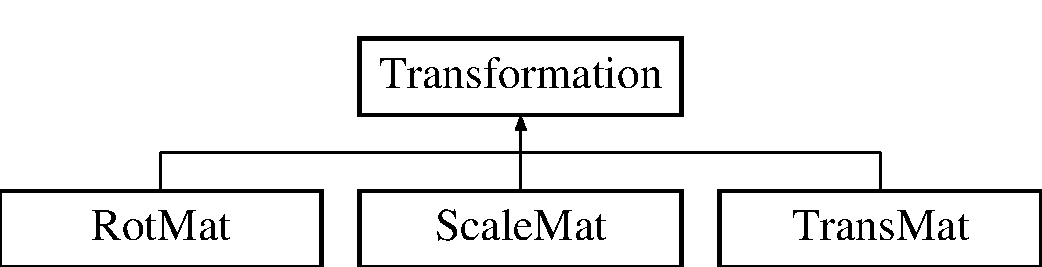
\includegraphics[height=2.000000cm]{class_transformation}
\end{center}
\end{figure}
\subsection*{Public Member Functions}
\begin{DoxyCompactItemize}
\item 
\hypertarget{class_transformation_ae6a57a1ee74ca1da1b8aef3d328a8772}{const \hyperlink{class_angel_1_1mat4}{Angel\-::mat4} \& {\bfseries Matrix} (void) const }\label{class_transformation_ae6a57a1ee74ca1da1b8aef3d328a8772}

\item 
\hypertarget{class_transformation_afdfbf48815a5b0d885f3b93f04cd2c66}{\hyperlink{class_angel_1_1mat4}{Angel\-::mat4} {\bfseries operator$\ast$} (const \hyperlink{class_angel_1_1mat4}{Angel\-::mat4} \&rhs) const }\label{class_transformation_afdfbf48815a5b0d885f3b93f04cd2c66}

\item 
\hypertarget{class_transformation_a85b923e0066365ef2e4aec3671396410}{\hyperlink{class_angel_1_1mat4}{Angel\-::mat4} {\bfseries operator$\ast$} (const \hyperlink{class_transformation}{Transformation} \&rhs) const }\label{class_transformation_a85b923e0066365ef2e4aec3671396410}

\end{DoxyCompactItemize}
\subsection*{Protected Attributes}
\begin{DoxyCompactItemize}
\item 
\hypertarget{class_transformation_a5f39fb578a1cdf78ca85efbd932d3834}{\hyperlink{class_angel_1_1mat4}{Angel\-::mat4} {\bfseries mat}}\label{class_transformation_a5f39fb578a1cdf78ca85efbd932d3834}

\end{DoxyCompactItemize}


\subsection{Detailed Description}


Definition at line 8 of file Transformation.\-hpp.



The documentation for this class was generated from the following files\-:\begin{DoxyCompactItemize}
\item 
Transformation.\-hpp\item 
Transformation.\-cpp\end{DoxyCompactItemize}

\hypertarget{class_trans_mat}{\section{Trans\-Mat Class Reference}
\label{class_trans_mat}\index{Trans\-Mat@{Trans\-Mat}}
}


Translations.  




{\ttfamily \#include $<$Transformation.\-hpp$>$}

Inheritance diagram for Trans\-Mat\-:\begin{figure}[H]
\begin{center}
\leavevmode
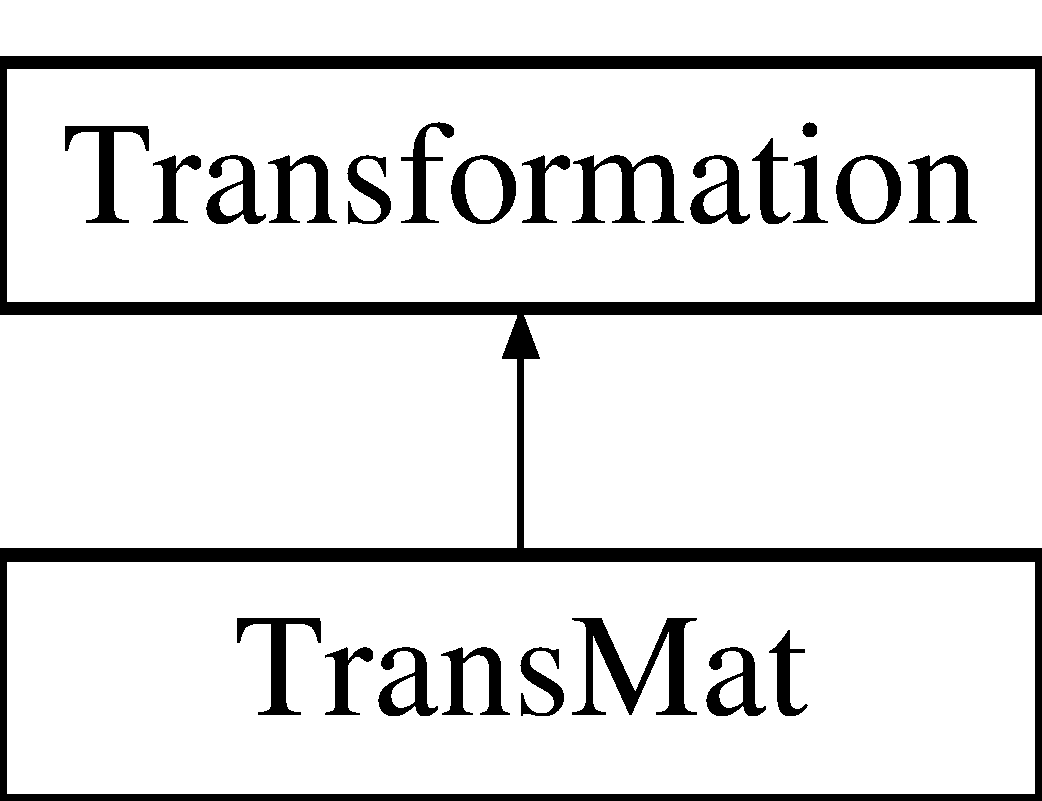
\includegraphics[height=2.000000cm]{class_trans_mat}
\end{center}
\end{figure}
\subsection*{Public Member Functions}
\begin{DoxyCompactItemize}
\item 
\hypertarget{class_trans_mat_a0a06e0dbfa09be06f0b8057283904b61}{const \hyperlink{class_trans_mat}{Trans\-Mat} \& {\bfseries Set\-X} (const float x)}\label{class_trans_mat_a0a06e0dbfa09be06f0b8057283904b61}

\item 
\hypertarget{class_trans_mat_a06c565961177be6b4945899d099eb7bc}{const \hyperlink{class_trans_mat}{Trans\-Mat} \& {\bfseries Set\-Y} (const float y)}\label{class_trans_mat_a06c565961177be6b4945899d099eb7bc}

\item 
\hypertarget{class_trans_mat_a9eaca6a2622a5820ee996409c477a54e}{const \hyperlink{class_trans_mat}{Trans\-Mat} \& {\bfseries Set\-Z} (const float z)}\label{class_trans_mat_a9eaca6a2622a5820ee996409c477a54e}

\item 
\hypertarget{class_trans_mat_a674c38b07b3f30ca46fdad9b3e699b77}{const \hyperlink{class_trans_mat}{Trans\-Mat} \& {\bfseries Set} (const float x, const float y, const float z)}\label{class_trans_mat_a674c38b07b3f30ca46fdad9b3e699b77}

\item 
\hypertarget{class_trans_mat_a5d6ab266be86788df753e5457afbe461}{const \hyperlink{class_trans_mat}{Trans\-Mat} \& {\bfseries Set} (const \hyperlink{struct_angel_1_1vec3}{Angel\-::vec3} \&arg)}\label{class_trans_mat_a5d6ab266be86788df753e5457afbe461}

\item 
\hypertarget{class_trans_mat_acaca3bb158b497ae5924fda662ff324d}{const \hyperlink{class_trans_mat}{Trans\-Mat} \& {\bfseries Delta} (const float x, const float y, const float z)}\label{class_trans_mat_acaca3bb158b497ae5924fda662ff324d}

\item 
\hypertarget{class_trans_mat_a1ba9395450677744c7c86d98f2d094d8}{const \hyperlink{class_trans_mat}{Trans\-Mat} \& {\bfseries Delta} (const \hyperlink{struct_angel_1_1vec3}{Angel\-::vec3} \&arg)}\label{class_trans_mat_a1ba9395450677744c7c86d98f2d094d8}

\item 
\hypertarget{class_transformation_ae6a57a1ee74ca1da1b8aef3d328a8772}{const \hyperlink{class_angel_1_1mat4}{Angel\-::mat4} \& {\bfseries Matrix} (void) const }\label{class_transformation_ae6a57a1ee74ca1da1b8aef3d328a8772}

\item 
\hypertarget{class_transformation_afdfbf48815a5b0d885f3b93f04cd2c66}{\hyperlink{class_angel_1_1mat4}{Angel\-::mat4} {\bfseries operator$\ast$} (const \hyperlink{class_angel_1_1mat4}{Angel\-::mat4} \&rhs) const }\label{class_transformation_afdfbf48815a5b0d885f3b93f04cd2c66}

\item 
\hypertarget{class_transformation_a85b923e0066365ef2e4aec3671396410}{\hyperlink{class_angel_1_1mat4}{Angel\-::mat4} {\bfseries operator$\ast$} (const \hyperlink{class_transformation}{Transformation} \&rhs) const }\label{class_transformation_a85b923e0066365ef2e4aec3671396410}

\end{DoxyCompactItemize}
\subsection*{Protected Attributes}
\begin{DoxyCompactItemize}
\item 
\hypertarget{class_transformation_a5f39fb578a1cdf78ca85efbd932d3834}{\hyperlink{class_angel_1_1mat4}{Angel\-::mat4} {\bfseries mat}}\label{class_transformation_a5f39fb578a1cdf78ca85efbd932d3834}

\end{DoxyCompactItemize}


\subsection{Detailed Description}
Translations. 

Definition at line 47 of file Transformation.\-hpp.



The documentation for this class was generated from the following files\-:\begin{DoxyCompactItemize}
\item 
Transformation.\-hpp\item 
Transformation.\-cpp\end{DoxyCompactItemize}

\hypertarget{struct_angel_1_1vec2}{\section{Angel\-:\-:vec2 Struct Reference}
\label{struct_angel_1_1vec2}\index{Angel\-::vec2@{Angel\-::vec2}}
}
\subsection*{Public Member Functions}
\begin{DoxyCompactItemize}
\item 
\hypertarget{struct_angel_1_1vec2_ab2463ddb6aaaa67251004b90f03530fa}{{\bfseries vec2} (G\-Lfloat s=G\-Lfloat(0.\-0))}\label{struct_angel_1_1vec2_ab2463ddb6aaaa67251004b90f03530fa}

\item 
\hypertarget{struct_angel_1_1vec2_a8e55cc0bb681ca7a747721cab122d830}{{\bfseries vec2} (G\-Lfloat x, G\-Lfloat y)}\label{struct_angel_1_1vec2_a8e55cc0bb681ca7a747721cab122d830}

\item 
\hypertarget{struct_angel_1_1vec2_aa2ec5b81c4b97019486b0595db6f35a1}{{\bfseries vec2} (const \hyperlink{struct_angel_1_1vec2}{vec2} \&v)}\label{struct_angel_1_1vec2_aa2ec5b81c4b97019486b0595db6f35a1}

\item 
\hypertarget{struct_angel_1_1vec2_a48235bf48a69717c273b72468d355244}{G\-Lfloat \& {\bfseries operator\mbox{[}$\,$\mbox{]}} (int i)}\label{struct_angel_1_1vec2_a48235bf48a69717c273b72468d355244}

\item 
\hypertarget{struct_angel_1_1vec2_a83725a082bca8ea73a2171bb4596c1bd}{const G\-Lfloat {\bfseries operator\mbox{[}$\,$\mbox{]}} (int i) const }\label{struct_angel_1_1vec2_a83725a082bca8ea73a2171bb4596c1bd}

\item 
\hypertarget{struct_angel_1_1vec2_a3b29693925c8026f75572dd13cefee5a}{\hyperlink{struct_angel_1_1vec2}{vec2} {\bfseries operator-\/} () const }\label{struct_angel_1_1vec2_a3b29693925c8026f75572dd13cefee5a}

\item 
\hypertarget{struct_angel_1_1vec2_a93606208e7b65d4bb8004f498b22934f}{\hyperlink{struct_angel_1_1vec2}{vec2} {\bfseries operator+} (const \hyperlink{struct_angel_1_1vec2}{vec2} \&v) const }\label{struct_angel_1_1vec2_a93606208e7b65d4bb8004f498b22934f}

\item 
\hypertarget{struct_angel_1_1vec2_a2d3d52e1b4693fdb860c2ef246e0d4d8}{\hyperlink{struct_angel_1_1vec2}{vec2} {\bfseries operator-\/} (const \hyperlink{struct_angel_1_1vec2}{vec2} \&v) const }\label{struct_angel_1_1vec2_a2d3d52e1b4693fdb860c2ef246e0d4d8}

\item 
\hypertarget{struct_angel_1_1vec2_ac5615b2494e3f8824f9fa127ba122b67}{\hyperlink{struct_angel_1_1vec2}{vec2} {\bfseries operator$\ast$} (const G\-Lfloat s) const }\label{struct_angel_1_1vec2_ac5615b2494e3f8824f9fa127ba122b67}

\item 
\hypertarget{struct_angel_1_1vec2_a3b4a9670b53342b870e3a14c8164c613}{\hyperlink{struct_angel_1_1vec2}{vec2} {\bfseries operator$\ast$} (const \hyperlink{struct_angel_1_1vec2}{vec2} \&v) const }\label{struct_angel_1_1vec2_a3b4a9670b53342b870e3a14c8164c613}

\item 
\hypertarget{struct_angel_1_1vec2_a522a6aaa64c361b86f6c2469cbd8ca92}{\hyperlink{struct_angel_1_1vec2}{vec2} {\bfseries operator/} (const G\-Lfloat s) const }\label{struct_angel_1_1vec2_a522a6aaa64c361b86f6c2469cbd8ca92}

\item 
\hypertarget{struct_angel_1_1vec2_aaa3b17cab0a568002fd965ef65e91653}{\hyperlink{struct_angel_1_1vec2}{vec2} \& {\bfseries operator+=} (const \hyperlink{struct_angel_1_1vec2}{vec2} \&v)}\label{struct_angel_1_1vec2_aaa3b17cab0a568002fd965ef65e91653}

\item 
\hypertarget{struct_angel_1_1vec2_ac48fa24fcdd901ab8748dda3361332f8}{\hyperlink{struct_angel_1_1vec2}{vec2} \& {\bfseries operator-\/=} (const \hyperlink{struct_angel_1_1vec2}{vec2} \&v)}\label{struct_angel_1_1vec2_ac48fa24fcdd901ab8748dda3361332f8}

\item 
\hypertarget{struct_angel_1_1vec2_a999ce51805c3c25a9a03039f05ce1492}{\hyperlink{struct_angel_1_1vec2}{vec2} \& {\bfseries operator$\ast$=} (const G\-Lfloat s)}\label{struct_angel_1_1vec2_a999ce51805c3c25a9a03039f05ce1492}

\item 
\hypertarget{struct_angel_1_1vec2_a8580b24c22b17ac08ab32841dcf03f45}{\hyperlink{struct_angel_1_1vec2}{vec2} \& {\bfseries operator$\ast$=} (const \hyperlink{struct_angel_1_1vec2}{vec2} \&v)}\label{struct_angel_1_1vec2_a8580b24c22b17ac08ab32841dcf03f45}

\item 
\hypertarget{struct_angel_1_1vec2_a6ea8be1d732aea09b0f3f16f61fa2ef7}{\hyperlink{struct_angel_1_1vec2}{vec2} \& {\bfseries operator/=} (const G\-Lfloat s)}\label{struct_angel_1_1vec2_a6ea8be1d732aea09b0f3f16f61fa2ef7}

\item 
\hypertarget{struct_angel_1_1vec2_a5c3d2082bcc18734fde3689dbc605104}{{\bfseries operator const G\-Lfloat $\ast$} () const }\label{struct_angel_1_1vec2_a5c3d2082bcc18734fde3689dbc605104}

\item 
\hypertarget{struct_angel_1_1vec2_a8989f46bc38bb87bc2f6ea81f66c8545}{{\bfseries operator G\-Lfloat $\ast$} ()}\label{struct_angel_1_1vec2_a8989f46bc38bb87bc2f6ea81f66c8545}

\end{DoxyCompactItemize}
\subsection*{Public Attributes}
\begin{DoxyCompactItemize}
\item 
\hypertarget{struct_angel_1_1vec2_ab99b91871c08bbf76bf4a5e554ccac8f}{G\-Lfloat {\bfseries x}}\label{struct_angel_1_1vec2_ab99b91871c08bbf76bf4a5e554ccac8f}

\item 
\hypertarget{struct_angel_1_1vec2_a9f0e4c33e7884eca47d771ccfd4ea0bd}{G\-Lfloat {\bfseries y}}\label{struct_angel_1_1vec2_a9f0e4c33e7884eca47d771ccfd4ea0bd}

\end{DoxyCompactItemize}
\subsection*{Friends}
\begin{DoxyCompactItemize}
\item 
\hypertarget{struct_angel_1_1vec2_a1f371c4b26f86deb4d296dfff8ff1fc1}{\hyperlink{struct_angel_1_1vec2}{vec2} {\bfseries operator$\ast$} (const G\-Lfloat s, const \hyperlink{struct_angel_1_1vec2}{vec2} \&v)}\label{struct_angel_1_1vec2_a1f371c4b26f86deb4d296dfff8ff1fc1}

\item 
\hypertarget{struct_angel_1_1vec2_a5533e582fe94db90861caa394494f2cf}{std\-::ostream \& {\bfseries operator$<$$<$} (std\-::ostream \&os, const \hyperlink{struct_angel_1_1vec2}{vec2} \&v)}\label{struct_angel_1_1vec2_a5533e582fe94db90861caa394494f2cf}

\item 
\hypertarget{struct_angel_1_1vec2_af8cf130207f2cf5866ac13049e956c75}{std\-::istream \& {\bfseries operator$>$$>$} (std\-::istream \&is, \hyperlink{struct_angel_1_1vec2}{vec2} \&v)}\label{struct_angel_1_1vec2_af8cf130207f2cf5866ac13049e956c75}

\end{DoxyCompactItemize}


\subsection{Detailed Description}


Definition at line 16 of file vec.\-hpp.



The documentation for this struct was generated from the following files\-:\begin{DoxyCompactItemize}
\item 
vec.\-hpp\item 
\hyperlink{vec_8cpp}{vec.\-cpp}\end{DoxyCompactItemize}

\hypertarget{struct_angel_1_1vec3}{\section{Angel\-:\-:vec3 Struct Reference}
\label{struct_angel_1_1vec3}\index{Angel\-::vec3@{Angel\-::vec3}}
}
\subsection*{Public Member Functions}
\begin{DoxyCompactItemize}
\item 
\hypertarget{struct_angel_1_1vec3_a420358f913d30a659761e3a86026cd59}{{\bfseries vec3} (G\-Lfloat s=G\-Lfloat(0.\-0))}\label{struct_angel_1_1vec3_a420358f913d30a659761e3a86026cd59}

\item 
\hypertarget{struct_angel_1_1vec3_a9970b9133cd349d038456ae7309fbeba}{{\bfseries vec3} (G\-Lfloat x, G\-Lfloat y, G\-Lfloat z)}\label{struct_angel_1_1vec3_a9970b9133cd349d038456ae7309fbeba}

\item 
\hypertarget{struct_angel_1_1vec3_a3af0b92e9cb01f0cda2f66c007e196c9}{{\bfseries vec3} (const \hyperlink{struct_angel_1_1vec3}{vec3} \&v)}\label{struct_angel_1_1vec3_a3af0b92e9cb01f0cda2f66c007e196c9}

\item 
\hypertarget{struct_angel_1_1vec3_a597ff15b14f6bd9e75382525f6da00bd}{{\bfseries vec3} (const \hyperlink{struct_angel_1_1vec2}{vec2} \&v, const float f)}\label{struct_angel_1_1vec3_a597ff15b14f6bd9e75382525f6da00bd}

\item 
\hypertarget{struct_angel_1_1vec3_a571e36d7c9542eb3464b8fde016d040d}{G\-Lfloat \& {\bfseries operator\mbox{[}$\,$\mbox{]}} (int i)}\label{struct_angel_1_1vec3_a571e36d7c9542eb3464b8fde016d040d}

\item 
\hypertarget{struct_angel_1_1vec3_ad78e907775d490a69aa879a34e7dfe5c}{const G\-Lfloat {\bfseries operator\mbox{[}$\,$\mbox{]}} (int i) const }\label{struct_angel_1_1vec3_ad78e907775d490a69aa879a34e7dfe5c}

\item 
\hypertarget{struct_angel_1_1vec3_a5ec954ef19e3d1ceed6ce25ebe32c3ee}{\hyperlink{struct_angel_1_1vec3}{vec3} {\bfseries operator-\/} () const }\label{struct_angel_1_1vec3_a5ec954ef19e3d1ceed6ce25ebe32c3ee}

\item 
\hypertarget{struct_angel_1_1vec3_a320586bc86a5abd0ac991a3e51485ef6}{\hyperlink{struct_angel_1_1vec3}{vec3} {\bfseries operator+} (const \hyperlink{struct_angel_1_1vec3}{vec3} \&v) const }\label{struct_angel_1_1vec3_a320586bc86a5abd0ac991a3e51485ef6}

\item 
\hypertarget{struct_angel_1_1vec3_a947a9982285c993f79d8ab3afc4da2c8}{\hyperlink{struct_angel_1_1vec3}{vec3} {\bfseries operator-\/} (const \hyperlink{struct_angel_1_1vec3}{vec3} \&v) const }\label{struct_angel_1_1vec3_a947a9982285c993f79d8ab3afc4da2c8}

\item 
\hypertarget{struct_angel_1_1vec3_aa2d45d74dee02720c82757f03263e8ae}{\hyperlink{struct_angel_1_1vec3}{vec3} {\bfseries operator$\ast$} (const G\-Lfloat s) const }\label{struct_angel_1_1vec3_aa2d45d74dee02720c82757f03263e8ae}

\item 
\hypertarget{struct_angel_1_1vec3_aa6709e55b49d756a9b00e038adc68438}{\hyperlink{struct_angel_1_1vec3}{vec3} {\bfseries operator$\ast$} (const \hyperlink{struct_angel_1_1vec3}{vec3} \&v) const }\label{struct_angel_1_1vec3_aa6709e55b49d756a9b00e038adc68438}

\item 
\hypertarget{struct_angel_1_1vec3_ab072ed9282da0217c26b8dae2c6bf978}{\hyperlink{struct_angel_1_1vec3}{vec3} {\bfseries operator/} (const G\-Lfloat s) const }\label{struct_angel_1_1vec3_ab072ed9282da0217c26b8dae2c6bf978}

\item 
\hypertarget{struct_angel_1_1vec3_abe9f854bc044ab4461882c635b197102}{\hyperlink{struct_angel_1_1vec3}{vec3} \& {\bfseries operator+=} (const \hyperlink{struct_angel_1_1vec3}{vec3} \&v)}\label{struct_angel_1_1vec3_abe9f854bc044ab4461882c635b197102}

\item 
\hypertarget{struct_angel_1_1vec3_ada518593451bbc8b9529ddd36284402f}{\hyperlink{struct_angel_1_1vec3}{vec3} \& {\bfseries operator-\/=} (const \hyperlink{struct_angel_1_1vec3}{vec3} \&v)}\label{struct_angel_1_1vec3_ada518593451bbc8b9529ddd36284402f}

\item 
\hypertarget{struct_angel_1_1vec3_ab825bec2ce97dc35aa4835758ec51270}{\hyperlink{struct_angel_1_1vec3}{vec3} \& {\bfseries operator$\ast$=} (const G\-Lfloat s)}\label{struct_angel_1_1vec3_ab825bec2ce97dc35aa4835758ec51270}

\item 
\hypertarget{struct_angel_1_1vec3_a54e75f1d64f773d99f0d5e80b031142b}{\hyperlink{struct_angel_1_1vec3}{vec3} \& {\bfseries operator$\ast$=} (const \hyperlink{struct_angel_1_1vec3}{vec3} \&v)}\label{struct_angel_1_1vec3_a54e75f1d64f773d99f0d5e80b031142b}

\item 
\hypertarget{struct_angel_1_1vec3_ae3ac03ba1ce7c8bbb8dfe07c7e0d06d9}{\hyperlink{struct_angel_1_1vec3}{vec3} \& {\bfseries operator/=} (const G\-Lfloat s)}\label{struct_angel_1_1vec3_ae3ac03ba1ce7c8bbb8dfe07c7e0d06d9}

\item 
\hypertarget{struct_angel_1_1vec3_a81f4a99d68722e756664907dcb07fb92}{{\bfseries operator const G\-Lfloat $\ast$} () const }\label{struct_angel_1_1vec3_a81f4a99d68722e756664907dcb07fb92}

\item 
\hypertarget{struct_angel_1_1vec3_ab92761f9bc4454117c1dd39a7d87c1b0}{{\bfseries operator G\-Lfloat $\ast$} ()}\label{struct_angel_1_1vec3_ab92761f9bc4454117c1dd39a7d87c1b0}

\end{DoxyCompactItemize}
\subsection*{Public Attributes}
\begin{DoxyCompactItemize}
\item 
\hypertarget{struct_angel_1_1vec3_a758dbe298cc37615770c30a73066253d}{G\-Lfloat {\bfseries x}}\label{struct_angel_1_1vec3_a758dbe298cc37615770c30a73066253d}

\item 
\hypertarget{struct_angel_1_1vec3_a02608203e694798c3118d5b55a0e0048}{G\-Lfloat {\bfseries y}}\label{struct_angel_1_1vec3_a02608203e694798c3118d5b55a0e0048}

\item 
\hypertarget{struct_angel_1_1vec3_afa2e7231c4170ddedb556ef5f7941cbc}{G\-Lfloat {\bfseries z}}\label{struct_angel_1_1vec3_afa2e7231c4170ddedb556ef5f7941cbc}

\end{DoxyCompactItemize}
\subsection*{Friends}
\begin{DoxyCompactItemize}
\item 
\hypertarget{struct_angel_1_1vec3_a1d78982e3d5969f2e9f98a536cfea9f7}{\hyperlink{struct_angel_1_1vec3}{vec3} {\bfseries operator$\ast$} (const G\-Lfloat s, const \hyperlink{struct_angel_1_1vec3}{vec3} \&v)}\label{struct_angel_1_1vec3_a1d78982e3d5969f2e9f98a536cfea9f7}

\item 
\hypertarget{struct_angel_1_1vec3_a3e8f4856b29a4320f185f9a9cf0f94bc}{std\-::ostream \& {\bfseries operator$<$$<$} (std\-::ostream \&os, const \hyperlink{struct_angel_1_1vec3}{vec3} \&v)}\label{struct_angel_1_1vec3_a3e8f4856b29a4320f185f9a9cf0f94bc}

\item 
\hypertarget{struct_angel_1_1vec3_ab705d3337286a4262e84bbbb0b694a56}{std\-::istream \& {\bfseries operator$>$$>$} (std\-::istream \&is, \hyperlink{struct_angel_1_1vec3}{vec3} \&v)}\label{struct_angel_1_1vec3_ab705d3337286a4262e84bbbb0b694a56}

\end{DoxyCompactItemize}


\subsection{Detailed Description}


Definition at line 61 of file vec.\-hpp.



The documentation for this struct was generated from the following files\-:\begin{DoxyCompactItemize}
\item 
vec.\-hpp\item 
\hyperlink{vec_8cpp}{vec.\-cpp}\end{DoxyCompactItemize}

\hypertarget{struct_angel_1_1vec4}{\section{Angel\-:\-:vec4 Struct Reference}
\label{struct_angel_1_1vec4}\index{Angel\-::vec4@{Angel\-::vec4}}
}
\subsection*{Public Member Functions}
\begin{DoxyCompactItemize}
\item 
\hypertarget{struct_angel_1_1vec4_afa13c9f342969e0ee740abbe3b7b8b4c}{{\bfseries vec4} (G\-Lfloat s=G\-Lfloat(0.\-0))}\label{struct_angel_1_1vec4_afa13c9f342969e0ee740abbe3b7b8b4c}

\item 
\hypertarget{struct_angel_1_1vec4_add0c2aa60bd9a4930c016fe08ffced70}{{\bfseries vec4} (G\-Lfloat x, G\-Lfloat y, G\-Lfloat z, G\-Lfloat w)}\label{struct_angel_1_1vec4_add0c2aa60bd9a4930c016fe08ffced70}

\item 
\hypertarget{struct_angel_1_1vec4_a72b386b6ebca67a90f47c12407e064f7}{{\bfseries vec4} (const \hyperlink{struct_angel_1_1vec4}{vec4} \&v)}\label{struct_angel_1_1vec4_a72b386b6ebca67a90f47c12407e064f7}

\item 
\hypertarget{struct_angel_1_1vec4_a48f563362bfe698603c365cc400bd99a}{{\bfseries vec4} (const \hyperlink{struct_angel_1_1vec3}{vec3} \&v, const float w=1.\-0)}\label{struct_angel_1_1vec4_a48f563362bfe698603c365cc400bd99a}

\item 
\hypertarget{struct_angel_1_1vec4_a8ac0995f9bba4d859ec9c46ed8e5d492}{{\bfseries vec4} (const \hyperlink{struct_angel_1_1vec2}{vec2} \&v, const float z, const float w)}\label{struct_angel_1_1vec4_a8ac0995f9bba4d859ec9c46ed8e5d492}

\item 
\hypertarget{struct_angel_1_1vec4_a1dc1b7daa6d5684466deee1ef8267910}{G\-Lfloat \& {\bfseries operator\mbox{[}$\,$\mbox{]}} (int i)}\label{struct_angel_1_1vec4_a1dc1b7daa6d5684466deee1ef8267910}

\item 
\hypertarget{struct_angel_1_1vec4_acc747bb9541dccb35a7953c91aa93ef9}{const G\-Lfloat {\bfseries operator\mbox{[}$\,$\mbox{]}} (int i) const }\label{struct_angel_1_1vec4_acc747bb9541dccb35a7953c91aa93ef9}

\item 
\hypertarget{struct_angel_1_1vec4_a7fbf327a3af8d45a22f6922993e71a03}{\hyperlink{struct_angel_1_1vec4}{vec4} {\bfseries operator-\/} () const }\label{struct_angel_1_1vec4_a7fbf327a3af8d45a22f6922993e71a03}

\item 
\hypertarget{struct_angel_1_1vec4_aa294368ad74207ccaf3d94a01fc48084}{\hyperlink{struct_angel_1_1vec4}{vec4} {\bfseries operator+} (const \hyperlink{struct_angel_1_1vec4}{vec4} \&v) const }\label{struct_angel_1_1vec4_aa294368ad74207ccaf3d94a01fc48084}

\item 
\hypertarget{struct_angel_1_1vec4_a6355469f6b5dfd9aad1abdb72c909d22}{\hyperlink{struct_angel_1_1vec4}{vec4} {\bfseries operator-\/} (const \hyperlink{struct_angel_1_1vec4}{vec4} \&v) const }\label{struct_angel_1_1vec4_a6355469f6b5dfd9aad1abdb72c909d22}

\item 
\hypertarget{struct_angel_1_1vec4_a92c877320dd47ffa15a0de898bd13638}{\hyperlink{struct_angel_1_1vec4}{vec4} {\bfseries operator$\ast$} (const G\-Lfloat s) const }\label{struct_angel_1_1vec4_a92c877320dd47ffa15a0de898bd13638}

\item 
\hypertarget{struct_angel_1_1vec4_add20f4c8f8e43a6efcc83a1aa8e1192a}{\hyperlink{struct_angel_1_1vec4}{vec4} {\bfseries operator$\ast$} (const \hyperlink{struct_angel_1_1vec4}{vec4} \&v) const }\label{struct_angel_1_1vec4_add20f4c8f8e43a6efcc83a1aa8e1192a}

\item 
\hypertarget{struct_angel_1_1vec4_a2110d1ac08fe09e785640e8219af23cf}{\hyperlink{struct_angel_1_1vec4}{vec4} {\bfseries operator/} (const G\-Lfloat s) const }\label{struct_angel_1_1vec4_a2110d1ac08fe09e785640e8219af23cf}

\item 
\hypertarget{struct_angel_1_1vec4_acae5e90e375b8fe265c39d4fabbf134d}{\hyperlink{struct_angel_1_1vec4}{vec4} \& {\bfseries operator+=} (const \hyperlink{struct_angel_1_1vec4}{vec4} \&v)}\label{struct_angel_1_1vec4_acae5e90e375b8fe265c39d4fabbf134d}

\item 
\hypertarget{struct_angel_1_1vec4_a2a861fc00ce40f6a6609ef631ddae21a}{\hyperlink{struct_angel_1_1vec4}{vec4} \& {\bfseries operator-\/=} (const \hyperlink{struct_angel_1_1vec4}{vec4} \&v)}\label{struct_angel_1_1vec4_a2a861fc00ce40f6a6609ef631ddae21a}

\item 
\hypertarget{struct_angel_1_1vec4_aab6ea06360d12b1e2962d6c4ea4dc639}{\hyperlink{struct_angel_1_1vec4}{vec4} \& {\bfseries operator$\ast$=} (const G\-Lfloat s)}\label{struct_angel_1_1vec4_aab6ea06360d12b1e2962d6c4ea4dc639}

\item 
\hypertarget{struct_angel_1_1vec4_a2035c8e93278408c05404b713346d92d}{\hyperlink{struct_angel_1_1vec4}{vec4} \& {\bfseries operator$\ast$=} (const \hyperlink{struct_angel_1_1vec4}{vec4} \&v)}\label{struct_angel_1_1vec4_a2035c8e93278408c05404b713346d92d}

\item 
\hypertarget{struct_angel_1_1vec4_aacad340463007e48c1674689787e6b47}{\hyperlink{struct_angel_1_1vec4}{vec4} \& {\bfseries operator/=} (const G\-Lfloat s)}\label{struct_angel_1_1vec4_aacad340463007e48c1674689787e6b47}

\item 
\hypertarget{struct_angel_1_1vec4_a71c7509461ea7152c6785bfbc811ab64}{{\bfseries operator const G\-Lfloat $\ast$} () const }\label{struct_angel_1_1vec4_a71c7509461ea7152c6785bfbc811ab64}

\item 
\hypertarget{struct_angel_1_1vec4_abe6702f74ba431df65da55aa0df6de16}{{\bfseries operator G\-Lfloat $\ast$} ()}\label{struct_angel_1_1vec4_abe6702f74ba431df65da55aa0df6de16}

\end{DoxyCompactItemize}
\subsection*{Public Attributes}
\begin{DoxyCompactItemize}
\item 
\hypertarget{struct_angel_1_1vec4_aaf7881acf82e877f889905a1573d36ad}{G\-Lfloat {\bfseries x}}\label{struct_angel_1_1vec4_aaf7881acf82e877f889905a1573d36ad}

\item 
\hypertarget{struct_angel_1_1vec4_a2396916bf1051ee7d6c11e6f2a539308}{G\-Lfloat {\bfseries y}}\label{struct_angel_1_1vec4_a2396916bf1051ee7d6c11e6f2a539308}

\item 
\hypertarget{struct_angel_1_1vec4_ab62654db1d62f75cb4d1bec9e4543797}{G\-Lfloat {\bfseries z}}\label{struct_angel_1_1vec4_ab62654db1d62f75cb4d1bec9e4543797}

\item 
\hypertarget{struct_angel_1_1vec4_a27752dffc3cd1ac7aa2fc72d40a84a48}{G\-Lfloat {\bfseries w}}\label{struct_angel_1_1vec4_a27752dffc3cd1ac7aa2fc72d40a84a48}

\end{DoxyCompactItemize}
\subsection*{Friends}
\begin{DoxyCompactItemize}
\item 
\hypertarget{struct_angel_1_1vec4_a18b1a91dc4c502220d099d6d85e504bc}{\hyperlink{struct_angel_1_1vec4}{vec4} {\bfseries operator$\ast$} (const G\-Lfloat s, const \hyperlink{struct_angel_1_1vec4}{vec4} \&v)}\label{struct_angel_1_1vec4_a18b1a91dc4c502220d099d6d85e504bc}

\item 
\hypertarget{struct_angel_1_1vec4_afadcf8884205c469256e4be7d96bfa12}{std\-::ostream \& {\bfseries operator$<$$<$} (std\-::ostream \&os, const \hyperlink{struct_angel_1_1vec4}{vec4} \&v)}\label{struct_angel_1_1vec4_afadcf8884205c469256e4be7d96bfa12}

\item 
\hypertarget{struct_angel_1_1vec4_ada396ae1c4ef513c6baf301f20f89bfa}{std\-::istream \& {\bfseries operator$>$$>$} (std\-::istream \&is, \hyperlink{struct_angel_1_1vec4}{vec4} \&v)}\label{struct_angel_1_1vec4_ada396ae1c4ef513c6baf301f20f89bfa}

\end{DoxyCompactItemize}


\subsection{Detailed Description}


Definition at line 111 of file vec.\-hpp.



The documentation for this struct was generated from the following files\-:\begin{DoxyCompactItemize}
\item 
vec.\-hpp\item 
\hyperlink{vec_8cpp}{vec.\-cpp}\end{DoxyCompactItemize}

\hypertarget{structwii_poll_data}{\section{wii\-Poll\-Data Struct Reference}
\label{structwii_poll_data}\index{wii\-Poll\-Data@{wii\-Poll\-Data}}
}
\subsection*{Public Attributes}
\begin{DoxyCompactItemize}
\item 
\hypertarget{structwii_poll_data_ad2a9be1946c67bd0da3de42dee26926a}{\hyperlink{struct_angel_1_1vec3}{Angel\-::vec3} {\bfseries bb\-\_\-magnitudes}}\label{structwii_poll_data_ad2a9be1946c67bd0da3de42dee26926a}

\item 
\hypertarget{structwii_poll_data_a9d7ad57a394cbae0d84285888a04c4ec}{\hyperlink{struct_angel_1_1vec3}{Angel\-::vec3} {\bfseries wr\-\_\-thetas}}\label{structwii_poll_data_a9d7ad57a394cbae0d84285888a04c4ec}

\item 
\hypertarget{structwii_poll_data_a794e2a15344966d546c3f02f3470a3af}{\hyperlink{struct_angel_1_1vec3}{Angel\-::vec3} {\bfseries wr\-\_\-rates}}\label{structwii_poll_data_a794e2a15344966d546c3f02f3470a3af}

\item 
\hypertarget{structwii_poll_data_af06c440335fec68bfa22d3601e050d2e}{bool {\bfseries Reset\-\_\-\-Camera}}\label{structwii_poll_data_af06c440335fec68bfa22d3601e050d2e}

\end{DoxyCompactItemize}


\subsection{Detailed Description}


Definition at line 7 of file Wii\-Util.\-h.



The documentation for this struct was generated from the following file\-:\begin{DoxyCompactItemize}
\item 
Wii\-Util.\-h\end{DoxyCompactItemize}

\chapter{File Documentation}
\hypertarget{_camera_8cpp}{\section{Camera.\-cpp File Reference}
\label{_camera_8cpp}\index{Camera.\-cpp@{Camera.\-cpp}}
}


Implementation for the \hyperlink{class_camera}{Camera} class.  


{\ttfamily \#include $<$stdexcept$>$}\\*
{\ttfamily \#include $<$iostream$>$}\\*
{\ttfamily \#include \char`\"{}mat.\-hpp\char`\"{}}\\*
{\ttfamily \#include \char`\"{}vec.\-hpp\char`\"{}}\\*
{\ttfamily \#include \char`\"{}Camera.\-hpp\char`\"{}}\\*
{\ttfamily \#include \char`\"{}globals.\-h\char`\"{}}\\*
{\ttfamily \#include \char`\"{}Timer.\-hpp\char`\"{}}\\*
\subsection*{Macros}
\begin{DoxyCompactItemize}
\item 
\#define \hyperlink{_camera_8cpp_a00e96bcc90e768c724477dbd2a3d9291}{R\-O\-T\-A\-T\-E\-\_\-\-O\-F\-F\-S\-E\-T}(V)~(V $\ast$ \-\_\-ctm.\-orbit.\-Matrix())
\begin{DoxyCompactList}\small\item\em R\-O\-T\-A\-T\-E\-\_\-\-O\-F\-F\-S\-E\-T is a macro which is used to normalize the six camera motion directions with respect to the current camera rotation. \end{DoxyCompactList}\end{DoxyCompactItemize}


\subsection{Detailed Description}
Implementation for the \hyperlink{class_camera}{Camera} class. \begin{DoxyAuthor}{Author}
John Huston 
\end{DoxyAuthor}
\begin{DoxyAuthor}{Authors}
John Huston, Nicholas St\-Pierre, Chris Compton 
\end{DoxyAuthor}
\begin{DoxyDate}{Date}
2012-\/12-\/20 
\end{DoxyDate}


Definition in file \hyperlink{_camera_8cpp_source}{Camera.\-cpp}.



\subsection{Macro Definition Documentation}
\hypertarget{_camera_8cpp_a00e96bcc90e768c724477dbd2a3d9291}{\index{Camera.\-cpp@{Camera.\-cpp}!R\-O\-T\-A\-T\-E\-\_\-\-O\-F\-F\-S\-E\-T@{R\-O\-T\-A\-T\-E\-\_\-\-O\-F\-F\-S\-E\-T}}
\index{R\-O\-T\-A\-T\-E\-\_\-\-O\-F\-F\-S\-E\-T@{R\-O\-T\-A\-T\-E\-\_\-\-O\-F\-F\-S\-E\-T}!Camera.cpp@{Camera.\-cpp}}
\subsubsection[{R\-O\-T\-A\-T\-E\-\_\-\-O\-F\-F\-S\-E\-T}]{\setlength{\rightskip}{0pt plus 5cm}\#define R\-O\-T\-A\-T\-E\-\_\-\-O\-F\-F\-S\-E\-T(
\begin{DoxyParamCaption}
\item[{}]{V}
\end{DoxyParamCaption}
)~(V $\ast$ \-\_\-ctm.\-orbit.\-Matrix())}}\label{_camera_8cpp_a00e96bcc90e768c724477dbd2a3d9291}


R\-O\-T\-A\-T\-E\-\_\-\-O\-F\-F\-S\-E\-T is a macro which is used to normalize the six camera motion directions with respect to the current camera rotation. 

It is used in heave(), sway() and surge(). 
\begin{DoxyParams}{Parameters}
{\em V} & a vec4 representing the movement offset vector. \\
\hline
\end{DoxyParams}
\begin{DoxyReturn}{Returns}
A rotated vec4. 
\end{DoxyReturn}


Definition at line 184 of file Camera.\-cpp.


\hypertarget{_camera_8hpp}{\section{Camera.\-hpp File Reference}
\label{_camera_8hpp}\index{Camera.\-hpp@{Camera.\-hpp}}
}


Header for the \hyperlink{class_camera}{Camera} class.  


{\ttfamily \#include $<$string$>$}\\*
{\ttfamily \#include \char`\"{}mat.\-hpp\char`\"{}}\\*
{\ttfamily \#include \char`\"{}vec.\-hpp\char`\"{}}\\*
{\ttfamily \#include \char`\"{}Object.\-hpp\char`\"{}}\\*
\subsection*{Classes}
\begin{DoxyCompactItemize}
\item 
class \hyperlink{class_camera}{Camera}
\begin{DoxyCompactList}\small\item\em The \hyperlink{class_camera}{Camera} class represents a logical camera in a model view, which posesses a current viewing angle and an absolute position in space as its state. \end{DoxyCompactList}\end{DoxyCompactItemize}


\subsection{Detailed Description}
Header for the \hyperlink{class_camera}{Camera} class. \begin{DoxyAuthor}{Author}
John Huston 
\end{DoxyAuthor}
\begin{DoxyAuthor}{Authors}
John Huston, Nicholas St\-Pierre, Chris Compton 
\end{DoxyAuthor}
\begin{DoxyDate}{Date}
2013-\/03-\/13 
\end{DoxyDate}


Definition in file \hyperlink{_camera_8hpp_source}{Camera.\-hpp}.


\hypertarget{_cameras_8cpp}{\section{Cameras.\-cpp File Reference}
\label{_cameras_8cpp}\index{Cameras.\-cpp@{Cameras.\-cpp}}
}


Implementation for the \hyperlink{class_cameras}{Cameras} class, which is a container for \hyperlink{class_camera}{Camera} objects.  


{\ttfamily \#include $<$cmath$>$}\\*
{\ttfamily \#include $<$vector$>$}\\*
{\ttfamily \#include $<$stdexcept$>$}\\*
{\ttfamily \#include \char`\"{}Camera.\-hpp\char`\"{}}\\*
{\ttfamily \#include \char`\"{}Cameras.\-hpp\char`\"{}}\\*
{\ttfamily \#include \char`\"{}globals.\-h\char`\"{}}\\*


\subsection{Detailed Description}
Implementation for the \hyperlink{class_cameras}{Cameras} class, which is a container for \hyperlink{class_camera}{Camera} objects. \begin{DoxyAuthor}{Author}
John Huston 
\end{DoxyAuthor}
\begin{DoxyAuthor}{Authors}
John Huston, Nicholas St\-Pierre, Chris Compton 
\end{DoxyAuthor}
\begin{DoxyDate}{Date}
2012-\/12-\/04 
\end{DoxyDate}


Definition in file \hyperlink{_cameras_8cpp_source}{Cameras.\-cpp}.


\hypertarget{_cameras_8hpp}{\section{Cameras.\-hpp File Reference}
\label{_cameras_8hpp}\index{Cameras.\-hpp@{Cameras.\-hpp}}
}


Header for the '\hyperlink{class_cameras}{Cameras}' class, a collection of \hyperlink{class_camera}{Camera} objects.  


{\ttfamily \#include $<$vector$>$}\\*
{\ttfamily \#include \char`\"{}Camera.\-hpp\char`\"{}}\\*
{\ttfamily \#include \char`\"{}Scene.\-hpp\char`\"{}}\\*
\subsection*{Classes}
\begin{DoxyCompactItemize}
\item 
class \hyperlink{class_cameras}{Cameras}
\begin{DoxyCompactList}\small\item\em The \hyperlink{class_cameras}{Cameras} class represents a group of logical cameras for a model view. Each camera possesses its own current viewing angle, and an absolute position in space. \end{DoxyCompactList}\end{DoxyCompactItemize}


\subsection{Detailed Description}
Header for the '\hyperlink{class_cameras}{Cameras}' class, a collection of \hyperlink{class_camera}{Camera} objects. \begin{DoxyAuthor}{Author}
John Huston 
\end{DoxyAuthor}
\begin{DoxyAuthor}{Authors}
John Huston, Nicholas St\-Pierre, Chris Compton 
\end{DoxyAuthor}
\begin{DoxyDate}{Date}
2012-\/12-\/04 
\end{DoxyDate}


Definition in file \hyperlink{_cameras_8hpp_source}{Cameras.\-hpp}.


\hypertarget{ds_8cpp}{\section{ds.\-cpp File Reference}
\label{ds_8cpp}\index{ds.\-cpp@{ds.\-cpp}}
}


Dual-\/shader demo.  


{\ttfamily \#include $<$S\-O\-I\-L.\-h$>$}\\*
{\ttfamily \#include \char`\"{}globals.\-h\char`\"{}}\\*
{\ttfamily \#include \char`\"{}platform.\-h\char`\"{}}\\*
{\ttfamily \#include \char`\"{}Camera.\-hpp\char`\"{}}\\*
{\ttfamily \#include \char`\"{}Cameras.\-hpp\char`\"{}}\\*
{\ttfamily \#include \char`\"{}Screen.\-hpp\char`\"{}}\\*
{\ttfamily \#include \char`\"{}Object.\-hpp\char`\"{}}\\*
{\ttfamily \#include \char`\"{}Timer.\-hpp\char`\"{}}\\*
{\ttfamily \#include \char`\"{}Scene.\-hpp\char`\"{}}\\*
{\ttfamily \#include \char`\"{}Engine.\-hpp\char`\"{}}\\*
{\ttfamily \#include \char`\"{}model.\-hpp\char`\"{}}\\*
{\ttfamily \#include \char`\"{}Init\-Shader.\-hpp\char`\"{}}\\*
{\ttfamily \#include \char`\"{}glut\-\_\-callbacks.\-h\char`\"{}}\\*
\subsection*{Functions}
\begin{DoxyCompactItemize}
\item 
\hypertarget{ds_8cpp_a02fd73d861ef2e4aabb38c0c9ff82947}{void \hyperlink{ds_8cpp_a02fd73d861ef2e4aabb38c0c9ff82947}{init} ()}\label{ds_8cpp_a02fd73d861ef2e4aabb38c0c9ff82947}

\begin{DoxyCompactList}\small\item\em Initialization\-: load and compile shaders, initialize camera(s), load models. \end{DoxyCompactList}\item 
\hypertarget{ds_8cpp_aeb94fbd457627182ceee7e505f432541}{void \hyperlink{ds_8cpp_aeb94fbd457627182ceee7e505f432541}{cleanup} (void)}\label{ds_8cpp_aeb94fbd457627182ceee7e505f432541}

\begin{DoxyCompactList}\small\item\em Cleans up our scene graph. \end{DoxyCompactList}\item 
\hypertarget{ds_8cpp_ad2e97e7b54d0bf35e406b91fbdd2f256}{void \hyperlink{ds_8cpp_ad2e97e7b54d0bf35e406b91fbdd2f256}{draw} (void)}\label{ds_8cpp_ad2e97e7b54d0bf35e406b91fbdd2f256}

\begin{DoxyCompactList}\small\item\em Implementation of drawing the display with regards to a single viewport. \end{DoxyCompactList}\item 
\hypertarget{ds_8cpp_a4ea013001a5fb47853d0fab8f8de35cd}{void \hyperlink{ds_8cpp_a4ea013001a5fb47853d0fab8f8de35cd}{display} (void)}\label{ds_8cpp_a4ea013001a5fb47853d0fab8f8de35cd}

\begin{DoxyCompactList}\small\item\em Display/\-Render the entire screen. \end{DoxyCompactList}\item 
\hypertarget{ds_8cpp_a01131b63acf241e9db91704d89ce15d2}{void \hyperlink{ds_8cpp_a01131b63acf241e9db91704d89ce15d2}{idle} (void)}\label{ds_8cpp_a01131b63acf241e9db91704d89ce15d2}

\begin{DoxyCompactList}\small\item\em Compute time since last idle, update camera positions, redisplay. \end{DoxyCompactList}\item 
int \hyperlink{ds_8cpp_a3c04138a5bfe5d72780bb7e82a18e627}{main} (int argc, char $\ast$$\ast$argv)
\begin{DoxyCompactList}\small\item\em This is a dual-\/shader demo! It looks very simple, but it illustrates quickly and effectively how to use two shaders. \end{DoxyCompactList}\end{DoxyCompactItemize}


\subsection{Detailed Description}
Dual-\/shader demo. \begin{DoxyAuthor}{Author}
John Huston 
\end{DoxyAuthor}
\begin{DoxyAuthor}{Authors}
John Huston, Greg Giannone 
\end{DoxyAuthor}
\begin{DoxyDate}{Date}
2013-\/02-\/20
\end{DoxyDate}
Work in progress! Based loosely on Ed Angel's tutorials. 

Definition in file \hyperlink{ds_8cpp_source}{ds.\-cpp}.



\subsection{Function Documentation}
\hypertarget{ds_8cpp_a3c04138a5bfe5d72780bb7e82a18e627}{\index{ds.\-cpp@{ds.\-cpp}!main@{main}}
\index{main@{main}!ds.cpp@{ds.\-cpp}}
\subsubsection[{main}]{\setlength{\rightskip}{0pt plus 5cm}int main (
\begin{DoxyParamCaption}
\item[{int}]{argc, }
\item[{char $\ast$$\ast$}]{argv}
\end{DoxyParamCaption}
)}}\label{ds_8cpp_a3c04138a5bfe5d72780bb7e82a18e627}


This is a dual-\/shader demo! It looks very simple, but it illustrates quickly and effectively how to use two shaders. 


\begin{DoxyParams}{Parameters}
{\em argc} & Not used. \\
\hline
{\em argv} & Not used. \\
\hline
\end{DoxyParams}
\begin{DoxyReturn}{Returns}
E\-X\-I\-T\-\_\-\-S\-U\-C\-C\-E\-S\-S. 
\end{DoxyReturn}


Definition at line 139 of file ds.\-cpp.


\hypertarget{_engine_8cpp}{\section{Engine.\-cpp File Reference}
\label{_engine_8cpp}\index{Engine.\-cpp@{Engine.\-cpp}}
}


Implementation for the \hyperlink{class_engine}{Engine} class.  


{\ttfamily \#include $<$stdexcept$>$}\\*
{\ttfamily \#include $<$string$>$}\\*
{\ttfamily \#include $<$map$>$}\\*
{\ttfamily \#include \char`\"{}Engine.\-hpp\char`\"{}}\\*
{\ttfamily \#include \char`\"{}Cameras.\-hpp\char`\"{}}\\*
{\ttfamily \#include \char`\"{}Scene.\-hpp\char`\"{}}\\*
{\ttfamily \#include \char`\"{}Screen.\-hpp\char`\"{}}\\*


\subsection{Detailed Description}
Implementation for the \hyperlink{class_engine}{Engine} class. \begin{DoxyAuthor}{Author}
John Huston 
\end{DoxyAuthor}
\begin{DoxyAuthor}{Authors}
\href{https://github.com/UMLComputerGraphics}{\tt https\-://github.\-com/\-U\-M\-L\-Computer\-Graphics} 
\end{DoxyAuthor}
\begin{DoxyDate}{Date}
2013-\/03-\/13 
\end{DoxyDate}


Definition in file \hyperlink{_engine_8cpp_source}{Engine.\-cpp}.


\hypertarget{_engine_8hpp}{\section{Engine.\-hpp File Reference}
\label{_engine_8hpp}\index{Engine.\-hpp@{Engine.\-hpp}}
}


Header for the \hyperlink{class_engine}{Engine} class.  


{\ttfamily \#include \char`\"{}Cameras.\-hpp\char`\"{}}\\*
{\ttfamily \#include \char`\"{}Scene.\-hpp\char`\"{}}\\*
{\ttfamily \#include \char`\"{}Screen.\-hpp\char`\"{}}\\*
{\ttfamily \#include $<$string$>$}\\*
{\ttfamily \#include $<$map$>$}\\*
\subsection*{Classes}
\begin{DoxyCompactItemize}
\item 
class \hyperlink{class_engine}{Engine}
\begin{DoxyCompactList}\small\item\em The \hyperlink{class_engine}{Engine} class is a singleton-\/style class which helps keep track of instances of important objects (for \hyperlink{class_cameras}{Cameras}, Objects, etc) as well as some settings and variables that would otherwise clog up global namespace. \end{DoxyCompactList}\end{DoxyCompactItemize}
\subsection*{Typedefs}
\begin{DoxyCompactItemize}
\item 
\hypertarget{_engine_8hpp_a35f3ec1606bb0642e48d2e62fea0d6a6}{typedef std\-::map$<$ std\-::string, \\*
bool $>$ \hyperlink{_engine_8hpp_a35f3ec1606bb0642e48d2e62fea0d6a6}{Settings\-Map}}\label{_engine_8hpp_a35f3ec1606bb0642e48d2e62fea0d6a6}

\begin{DoxyCompactList}\small\item\em An alias for the type used by the Settings Map. \end{DoxyCompactList}\end{DoxyCompactItemize}


\subsection{Detailed Description}
Header for the \hyperlink{class_engine}{Engine} class. \begin{DoxyAuthor}{Author}
John Huston 
\end{DoxyAuthor}
\begin{DoxyAuthor}{Authors}
\href{https://github.com/UMLComputerGraphics}{\tt https\-://github.\-com/\-U\-M\-L\-Computer\-Graphics} 
\end{DoxyAuthor}
\begin{DoxyDate}{Date}
2013-\/03-\/13 
\end{DoxyDate}


Definition in file \hyperlink{_engine_8hpp_source}{Engine.\-hpp}.


\hypertarget{globals_8h}{\section{globals.\-h File Reference}
\label{globals_8h}\index{globals.\-h@{globals.\-h}}
}


Useful global constants, macros, debugging utilities and preprocessor settings.  


{\ttfamily \#include $<$cmath$>$}\\*
\subsection*{Macros}
\begin{DoxyCompactItemize}
\item 
\#define \hyperlink{globals_8h_a7bf0b4b8b3cf2f13f25573b3e151ed88}{D\-E\-G\-R\-E\-E\-S\-\_\-\-T\-O\-\_\-\-R\-A\-D\-I\-A\-N\-S}~(M\-\_\-\-P\-I/180)
\begin{DoxyCompactList}\small\item\em A constant factor of conversion for Degrees to Radians. \end{DoxyCompactList}\item 
\#define \hyperlink{globals_8h_a514396dd60fa0621c83072091fb2a0cd}{S\-Q\-R\-T2}~(1.\-41421356237)
\begin{DoxyCompactList}\small\item\em A constant for the square root of 2. \end{DoxyCompactList}\item 
\#define \hyperlink{globals_8h_ae42978afd835c3a1f70d409a1b5f5a39}{S\-Q\-R\-T3}~(1.\-73205080757)
\begin{DoxyCompactList}\small\item\em A constant for the square root of 3. \end{DoxyCompactList}\item 
\#define \hyperlink{globals_8h_a7bbc032e1437a7a73f8d3eb2d93d9c6d}{P\-O\-W5}(X)~((X)$\ast$(X)$\ast$(X)$\ast$(X)$\ast$(X))
\begin{DoxyCompactList}\small\item\em \hyperlink{globals_8h_a7bbc032e1437a7a73f8d3eb2d93d9c6d}{P\-O\-W5(\-X)} returns X$^\wedge$5. \end{DoxyCompactList}\item 
\hypertarget{globals_8h_ad72dbcf6d0153db1b8d8a58001feed83}{\#define \hyperlink{globals_8h_ad72dbcf6d0153db1b8d8a58001feed83}{D\-E\-B\-U\-G}~false}\label{globals_8h_ad72dbcf6d0153db1b8d8a58001feed83}

\begin{DoxyCompactList}\small\item\em D\-E\-B\-U\-G Controls whether or not extra D\-E\-B\-U\-G messages are printed out. \end{DoxyCompactList}\item 
\hypertarget{globals_8h_ab5f638ed0890579dbe0522227610af64}{\#define \hyperlink{globals_8h_ab5f638ed0890579dbe0522227610af64}{D\-E\-B\-U\-G\-\_\-\-M\-O\-T\-I\-O\-N}~(false)}\label{globals_8h_ab5f638ed0890579dbe0522227610af64}

\begin{DoxyCompactList}\small\item\em D\-E\-B\-U\-G\-\_\-\-M\-O\-T\-I\-O\-N controls some additional debug messages for acceleration/velocity. \end{DoxyCompactList}\end{DoxyCompactItemize}
\subsection*{Variables}
\begin{DoxyCompactItemize}
\item 
\hypertarget{globals_8h_ad90a072ea1667bc81e21b726aefbcff1}{const float \hyperlink{globals_8h_ad90a072ea1667bc81e21b726aefbcff1}{D\-I\-V\-I\-D\-E\-\_\-\-B\-Y\-\_\-\-Z\-E\-R\-O\-\_\-\-T\-O\-L\-E\-R\-A\-N\-C\-E} = float( 1.\-0e-\/07 )}\label{globals_8h_ad90a072ea1667bc81e21b726aefbcff1}

\begin{DoxyCompactList}\small\item\em How close can a number be to zero before it should be considered 'zero'? \end{DoxyCompactList}\item 
static const bool \hyperlink{globals_8h_afbd48522ecf2a24bf2adca81f5a0e616}{P\-O\-S\-T\-M\-U\-L\-T} = true
\begin{DoxyCompactList}\small\item\em defines if we are, or are not using a Post-\/\-Multiplication system. \end{DoxyCompactList}\item 
static const bool \hyperlink{globals_8h_a6606f2e98acd846ae52f6cd2f7585d22}{P\-R\-E\-M\-U\-L\-T} = false
\begin{DoxyCompactList}\small\item\em defines if we are, or are not using a Pre-\/\-Multiplication system. \end{DoxyCompactList}\end{DoxyCompactItemize}


\subsection{Detailed Description}
Useful global constants, macros, debugging utilities and preprocessor settings. \begin{DoxyAuthor}{Author}
John Huston 
\end{DoxyAuthor}
\begin{DoxyDate}{Date}
2013-\/03-\/13 
\end{DoxyDate}


Definition in file \hyperlink{globals_8h_source}{globals.\-h}.



\subsection{Macro Definition Documentation}
\hypertarget{globals_8h_a7bf0b4b8b3cf2f13f25573b3e151ed88}{\index{globals.\-h@{globals.\-h}!D\-E\-G\-R\-E\-E\-S\-\_\-\-T\-O\-\_\-\-R\-A\-D\-I\-A\-N\-S@{D\-E\-G\-R\-E\-E\-S\-\_\-\-T\-O\-\_\-\-R\-A\-D\-I\-A\-N\-S}}
\index{D\-E\-G\-R\-E\-E\-S\-\_\-\-T\-O\-\_\-\-R\-A\-D\-I\-A\-N\-S@{D\-E\-G\-R\-E\-E\-S\-\_\-\-T\-O\-\_\-\-R\-A\-D\-I\-A\-N\-S}!globals.h@{globals.\-h}}
\subsubsection[{D\-E\-G\-R\-E\-E\-S\-\_\-\-T\-O\-\_\-\-R\-A\-D\-I\-A\-N\-S}]{\setlength{\rightskip}{0pt plus 5cm}\#define D\-E\-G\-R\-E\-E\-S\-\_\-\-T\-O\-\_\-\-R\-A\-D\-I\-A\-N\-S~(M\-\_\-\-P\-I/180)}}\label{globals_8h_a7bf0b4b8b3cf2f13f25573b3e151ed88}


A constant factor of conversion for Degrees to Radians. 



Definition at line 14 of file globals.\-h.

\hypertarget{globals_8h_a7bbc032e1437a7a73f8d3eb2d93d9c6d}{\index{globals.\-h@{globals.\-h}!P\-O\-W5@{P\-O\-W5}}
\index{P\-O\-W5@{P\-O\-W5}!globals.h@{globals.\-h}}
\subsubsection[{P\-O\-W5}]{\setlength{\rightskip}{0pt plus 5cm}\#define P\-O\-W5(
\begin{DoxyParamCaption}
\item[{}]{X}
\end{DoxyParamCaption}
)~((X)$\ast$(X)$\ast$(X)$\ast$(X)$\ast$(X))}}\label{globals_8h_a7bbc032e1437a7a73f8d3eb2d93d9c6d}


\hyperlink{globals_8h_a7bbc032e1437a7a73f8d3eb2d93d9c6d}{P\-O\-W5(\-X)} returns X$^\wedge$5. 

It's quicker than pow(x,5)! 

Definition at line 20 of file globals.\-h.

\hypertarget{globals_8h_a514396dd60fa0621c83072091fb2a0cd}{\index{globals.\-h@{globals.\-h}!S\-Q\-R\-T2@{S\-Q\-R\-T2}}
\index{S\-Q\-R\-T2@{S\-Q\-R\-T2}!globals.h@{globals.\-h}}
\subsubsection[{S\-Q\-R\-T2}]{\setlength{\rightskip}{0pt plus 5cm}\#define S\-Q\-R\-T2~(1.\-41421356237)}}\label{globals_8h_a514396dd60fa0621c83072091fb2a0cd}


A constant for the square root of 2. 



Definition at line 16 of file globals.\-h.

\hypertarget{globals_8h_ae42978afd835c3a1f70d409a1b5f5a39}{\index{globals.\-h@{globals.\-h}!S\-Q\-R\-T3@{S\-Q\-R\-T3}}
\index{S\-Q\-R\-T3@{S\-Q\-R\-T3}!globals.h@{globals.\-h}}
\subsubsection[{S\-Q\-R\-T3}]{\setlength{\rightskip}{0pt plus 5cm}\#define S\-Q\-R\-T3~(1.\-73205080757)}}\label{globals_8h_ae42978afd835c3a1f70d409a1b5f5a39}


A constant for the square root of 3. 



Definition at line 18 of file globals.\-h.



\subsection{Variable Documentation}
\hypertarget{globals_8h_afbd48522ecf2a24bf2adca81f5a0e616}{\index{globals.\-h@{globals.\-h}!P\-O\-S\-T\-M\-U\-L\-T@{P\-O\-S\-T\-M\-U\-L\-T}}
\index{P\-O\-S\-T\-M\-U\-L\-T@{P\-O\-S\-T\-M\-U\-L\-T}!globals.h@{globals.\-h}}
\subsubsection[{P\-O\-S\-T\-M\-U\-L\-T}]{\setlength{\rightskip}{0pt plus 5cm}const bool P\-O\-S\-T\-M\-U\-L\-T = true\hspace{0.3cm}{\ttfamily [static]}}}\label{globals_8h_afbd48522ecf2a24bf2adca81f5a0e616}


defines if we are, or are not using a Post-\/\-Multiplication system. 



Definition at line 43 of file globals.\-h.

\hypertarget{globals_8h_a6606f2e98acd846ae52f6cd2f7585d22}{\index{globals.\-h@{globals.\-h}!P\-R\-E\-M\-U\-L\-T@{P\-R\-E\-M\-U\-L\-T}}
\index{P\-R\-E\-M\-U\-L\-T@{P\-R\-E\-M\-U\-L\-T}!globals.h@{globals.\-h}}
\subsubsection[{P\-R\-E\-M\-U\-L\-T}]{\setlength{\rightskip}{0pt plus 5cm}const bool P\-R\-E\-M\-U\-L\-T = false\hspace{0.3cm}{\ttfamily [static]}}}\label{globals_8h_a6606f2e98acd846ae52f6cd2f7585d22}


defines if we are, or are not using a Pre-\/\-Multiplication system. 



Definition at line 45 of file globals.\-h.


\hypertarget{glut__callbacks_8cpp}{\section{glut\-\_\-callbacks.\-cpp File Reference}
\label{glut__callbacks_8cpp}\index{glut\-\_\-callbacks.\-cpp@{glut\-\_\-callbacks.\-cpp}}
}


glut\-\_\-callbacks provides function declarations for a set of functions commonly used across multiple binaries for keyboard, mouse and other G\-L\-U\-T callback functions.  


{\ttfamily \#include \char`\"{}globals.\-h\char`\"{}}\\*
{\ttfamily \#include \char`\"{}Camera.\-hpp\char`\"{}}\\*
{\ttfamily \#include \char`\"{}Scene.\-hpp\char`\"{}}\\*
{\ttfamily \#include \char`\"{}Screen.\-hpp\char`\"{}}\\*
{\ttfamily \#include \char`\"{}Engine.\-hpp\char`\"{}}\\*
{\ttfamily \#include $<$sstream$>$}\\*
\subsection*{Functions}
\begin{DoxyCompactItemize}
\item 
void \hyperlink{glut__callbacks_8cpp_a254e97178a2df1da3e435a01f778e475}{keylift} (unsigned char key, int x, int y)
\begin{DoxyCompactList}\small\item\em keylift is registered as a G\-L\-U\-T callback for when a user releases a depressed key. \end{DoxyCompactList}\item 
void \hyperlink{glut__callbacks_8cpp_aef7ba2f69afb2d954545f64c7fe24b14}{keyboard} (unsigned char key, int x, int y)
\begin{DoxyCompactList}\small\item\em keyboard is a callback registered with G\-L\-U\-T. \end{DoxyCompactList}\item 
void \hyperlink{glut__callbacks_8cpp_a6f3a97ed034be467bc035242d2486e00}{keyboard\-\_\-ctrl} (int key, int x, int y)
\begin{DoxyCompactList}\small\item\em keyboard\-\_\-ctrl is registered as a G\-L\-U\-T callback. \end{DoxyCompactList}\item 
void \hyperlink{glut__callbacks_8cpp_ac76a5d78172a826cd6ee9512b89a86c0}{mouse} (int button, int state, int x, int y)
\begin{DoxyCompactList}\small\item\em mouse is registered as a G\-L\-U\-T callback. \end{DoxyCompactList}\item 
void \hyperlink{glut__callbacks_8cpp_ad373689e6b9dcfe1b99692b43a759d40}{mouseroll} (int x, int y)
\begin{DoxyCompactList}\small\item\em mouseroll is registered as a G\-L\-U\-T callback. \end{DoxyCompactList}\item 
void \hyperlink{glut__callbacks_8cpp_af04567427614c77718ed14b8450a3438}{mouselook} (int x, int y)
\begin{DoxyCompactList}\small\item\em mouselook is registered as a G\-L\-U\-T callback. \end{DoxyCompactList}\item 
void \hyperlink{glut__callbacks_8cpp_ace248343c050c709b645c42012d68f18}{resize\-Event} (int width, int height)
\begin{DoxyCompactList}\small\item\em resize\-Event is registered as a glut callback for when the screen is resized. \end{DoxyCompactList}\end{DoxyCompactItemize}


\subsection{Detailed Description}
glut\-\_\-callbacks provides function declarations for a set of functions commonly used across multiple binaries for keyboard, mouse and other G\-L\-U\-T callback functions. \begin{DoxyAuthor}{Author}
John Huston 
\end{DoxyAuthor}
\begin{DoxyAuthor}{Authors}
John Huston, Nick St.\-Pierre, Chris Compton 
\end{DoxyAuthor}
\begin{DoxyDate}{Date}
2013-\/03-\/13 
\end{DoxyDate}


Definition in file \hyperlink{glut__callbacks_8cpp_source}{glut\-\_\-callbacks.\-cpp}.



\subsection{Function Documentation}
\hypertarget{glut__callbacks_8cpp_aef7ba2f69afb2d954545f64c7fe24b14}{\index{glut\-\_\-callbacks.\-cpp@{glut\-\_\-callbacks.\-cpp}!keyboard@{keyboard}}
\index{keyboard@{keyboard}!glut_callbacks.cpp@{glut\-\_\-callbacks.\-cpp}}
\subsubsection[{keyboard}]{\setlength{\rightskip}{0pt plus 5cm}void keyboard (
\begin{DoxyParamCaption}
\item[{unsigned char}]{key, }
\item[{int}]{x, }
\item[{int}]{y}
\end{DoxyParamCaption}
)}}\label{glut__callbacks_8cpp_aef7ba2f69afb2d954545f64c7fe24b14}


keyboard is a callback registered with G\-L\-U\-T. 

It handles (surprise!) keyboard input.


\begin{DoxyParams}{Parameters}
{\em key} & The key pressed by the user. \\
\hline
{\em x} & The x coordinate of the mouse when the key was pressed. \\
\hline
{\em y} & The y coordinate of the mouse when the key was pressed. \\
\hline
\end{DoxyParams}


Definition at line 66 of file glut\-\_\-callbacks.\-cpp.

\hypertarget{glut__callbacks_8cpp_a6f3a97ed034be467bc035242d2486e00}{\index{glut\-\_\-callbacks.\-cpp@{glut\-\_\-callbacks.\-cpp}!keyboard\-\_\-ctrl@{keyboard\-\_\-ctrl}}
\index{keyboard\-\_\-ctrl@{keyboard\-\_\-ctrl}!glut_callbacks.cpp@{glut\-\_\-callbacks.\-cpp}}
\subsubsection[{keyboard\-\_\-ctrl}]{\setlength{\rightskip}{0pt plus 5cm}void keyboard\-\_\-ctrl (
\begin{DoxyParamCaption}
\item[{int}]{key, }
\item[{int}]{x, }
\item[{int}]{y}
\end{DoxyParamCaption}
)}}\label{glut__callbacks_8cpp_a6f3a97ed034be467bc035242d2486e00}


keyboard\-\_\-ctrl is registered as a G\-L\-U\-T callback. 

It is responsible for catching when special keys are pressed.


\begin{DoxyParams}{Parameters}
{\em key} & The key pressed. \\
\hline
{\em x} & The x coordinate of the mouse when the key was pressed. \\
\hline
{\em y} & The y coordinate of the mouse when the key was pressed. \\
\hline
\end{DoxyParams}


Definition at line 167 of file glut\-\_\-callbacks.\-cpp.

\hypertarget{glut__callbacks_8cpp_a254e97178a2df1da3e435a01f778e475}{\index{glut\-\_\-callbacks.\-cpp@{glut\-\_\-callbacks.\-cpp}!keylift@{keylift}}
\index{keylift@{keylift}!glut_callbacks.cpp@{glut\-\_\-callbacks.\-cpp}}
\subsubsection[{keylift}]{\setlength{\rightskip}{0pt plus 5cm}void keylift (
\begin{DoxyParamCaption}
\item[{unsigned char}]{key, }
\item[{int}]{x, }
\item[{int}]{y}
\end{DoxyParamCaption}
)}}\label{glut__callbacks_8cpp_a254e97178a2df1da3e435a01f778e475}


keylift is registered as a G\-L\-U\-T callback for when a user releases a depressed key. 


\begin{DoxyParams}{Parameters}
{\em key} & The key that was lifted. \\
\hline
{\em x} & The x coordinate of the mouse at the time the key was released. \\
\hline
{\em y} & The y coordinate of the mouse at the time the key was released. \\
\hline
\end{DoxyParams}


Definition at line 29 of file glut\-\_\-callbacks.\-cpp.

\hypertarget{glut__callbacks_8cpp_ac76a5d78172a826cd6ee9512b89a86c0}{\index{glut\-\_\-callbacks.\-cpp@{glut\-\_\-callbacks.\-cpp}!mouse@{mouse}}
\index{mouse@{mouse}!glut_callbacks.cpp@{glut\-\_\-callbacks.\-cpp}}
\subsubsection[{mouse}]{\setlength{\rightskip}{0pt plus 5cm}void mouse (
\begin{DoxyParamCaption}
\item[{int}]{button, }
\item[{int}]{state, }
\item[{int}]{x, }
\item[{int}]{y}
\end{DoxyParamCaption}
)}}\label{glut__callbacks_8cpp_ac76a5d78172a826cd6ee9512b89a86c0}


mouse is registered as a G\-L\-U\-T callback. 

It handles input from, primarily, the scrollwheel.


\begin{DoxyParams}{Parameters}
{\em button} & The mouse button being pressed. \\
\hline
{\em state} & the state of the aforementioned mouse button. \\
\hline
{\em x} & the x coordinate of the mouse. \\
\hline
{\em y} & the y coordinate of the mouse. \\
\hline
\end{DoxyParams}


Definition at line 219 of file glut\-\_\-callbacks.\-cpp.

\hypertarget{glut__callbacks_8cpp_af04567427614c77718ed14b8450a3438}{\index{glut\-\_\-callbacks.\-cpp@{glut\-\_\-callbacks.\-cpp}!mouselook@{mouselook}}
\index{mouselook@{mouselook}!glut_callbacks.cpp@{glut\-\_\-callbacks.\-cpp}}
\subsubsection[{mouselook}]{\setlength{\rightskip}{0pt plus 5cm}void mouselook (
\begin{DoxyParamCaption}
\item[{int}]{x, }
\item[{int}]{y}
\end{DoxyParamCaption}
)}}\label{glut__callbacks_8cpp_af04567427614c77718ed14b8450a3438}


mouselook is registered as a G\-L\-U\-T callback. 

mouselook implements F\-P\-S-\/like controls where the camera moves proportional to the direction of the mouse.


\begin{DoxyParams}{Parameters}
{\em x} & the x coordinate of the mouse pointer. \\
\hline
{\em y} & the y coordinate of the mouse pointer. \\
\hline
\end{DoxyParams}


Definition at line 265 of file glut\-\_\-callbacks.\-cpp.

\hypertarget{glut__callbacks_8cpp_ad373689e6b9dcfe1b99692b43a759d40}{\index{glut\-\_\-callbacks.\-cpp@{glut\-\_\-callbacks.\-cpp}!mouseroll@{mouseroll}}
\index{mouseroll@{mouseroll}!glut_callbacks.cpp@{glut\-\_\-callbacks.\-cpp}}
\subsubsection[{mouseroll}]{\setlength{\rightskip}{0pt plus 5cm}void mouseroll (
\begin{DoxyParamCaption}
\item[{int}]{x, }
\item[{int}]{y}
\end{DoxyParamCaption}
)}}\label{glut__callbacks_8cpp_ad373689e6b9dcfe1b99692b43a759d40}


mouseroll is registered as a G\-L\-U\-T callback. 

mouseroll is called when the mouse is moved while a button is depressed. It is used here to implement barrel-\/rolls while left-\/clicking.


\begin{DoxyParams}{Parameters}
{\em x} & the x coordinate of the mouse pointer. \\
\hline
{\em y} & the y coordinate of the mouse pointer. \\
\hline
\end{DoxyParams}


Definition at line 245 of file glut\-\_\-callbacks.\-cpp.

\hypertarget{glut__callbacks_8cpp_ace248343c050c709b645c42012d68f18}{\index{glut\-\_\-callbacks.\-cpp@{glut\-\_\-callbacks.\-cpp}!resize\-Event@{resize\-Event}}
\index{resize\-Event@{resize\-Event}!glut_callbacks.cpp@{glut\-\_\-callbacks.\-cpp}}
\subsubsection[{resize\-Event}]{\setlength{\rightskip}{0pt plus 5cm}void resize\-Event (
\begin{DoxyParamCaption}
\item[{int}]{width, }
\item[{int}]{height}
\end{DoxyParamCaption}
)}}\label{glut__callbacks_8cpp_ace248343c050c709b645c42012d68f18}


resize\-Event is registered as a glut callback for when the screen is resized. 

It instructs the screen object of the new size, which informs all of the children cameras to recompute their aspect ratios, viewport positions, and so on.

We also warp the pointer to the center of the screen, for compatibility with mouselook( void ).


\begin{DoxyParams}{Parameters}
{\em width} & The new width of the window. \\
\hline
{\em height} & The new height of the window.\\
\hline
\end{DoxyParams}
\begin{DoxyReturn}{Returns}
void. 
\end{DoxyReturn}


Definition at line 299 of file glut\-\_\-callbacks.\-cpp.


\hypertarget{glut__callbacks_8h}{\section{glut\-\_\-callbacks.\-h File Reference}
\label{glut__callbacks_8h}\index{glut\-\_\-callbacks.\-h@{glut\-\_\-callbacks.\-h}}
}


\hyperlink{glut__callbacks_8h}{glut\-\_\-callbacks.\-h} provides function declarations for a set of functions commonly used across multiple binaries for keyboard, mouse and other G\-L\-U\-T callback functions.  


\subsection*{Functions}
\begin{DoxyCompactItemize}
\item 
void \hyperlink{glut__callbacks_8h_a254e97178a2df1da3e435a01f778e475}{keylift} (unsigned char key, int x, int y)
\begin{DoxyCompactList}\small\item\em keylift is registered as a G\-L\-U\-T callback for when a user releases a depressed key. \end{DoxyCompactList}\item 
void \hyperlink{glut__callbacks_8h_aef7ba2f69afb2d954545f64c7fe24b14}{keyboard} (unsigned char key, int x, int y)
\begin{DoxyCompactList}\small\item\em keyboard is a callback registered with G\-L\-U\-T. \end{DoxyCompactList}\item 
void \hyperlink{glut__callbacks_8h_a6f3a97ed034be467bc035242d2486e00}{keyboard\-\_\-ctrl} (int key, int x, int y)
\begin{DoxyCompactList}\small\item\em keyboard\-\_\-ctrl is registered as a G\-L\-U\-T callback. \end{DoxyCompactList}\item 
void \hyperlink{glut__callbacks_8h_ac76a5d78172a826cd6ee9512b89a86c0}{mouse} (int button, int state, int x, int y)
\begin{DoxyCompactList}\small\item\em mouse is registered as a G\-L\-U\-T callback. \end{DoxyCompactList}\item 
void \hyperlink{glut__callbacks_8h_ad373689e6b9dcfe1b99692b43a759d40}{mouseroll} (int x, int y)
\begin{DoxyCompactList}\small\item\em mouseroll is registered as a G\-L\-U\-T callback. \end{DoxyCompactList}\item 
void \hyperlink{glut__callbacks_8h_af04567427614c77718ed14b8450a3438}{mouselook} (int x, int y)
\begin{DoxyCompactList}\small\item\em mouselook is registered as a G\-L\-U\-T callback. \end{DoxyCompactList}\item 
void \hyperlink{glut__callbacks_8h_ace248343c050c709b645c42012d68f18}{resize\-Event} (int width, int height)
\begin{DoxyCompactList}\small\item\em resize\-Event is registered as a glut callback for when the screen is resized. \end{DoxyCompactList}\end{DoxyCompactItemize}


\subsection{Detailed Description}
\hyperlink{glut__callbacks_8h}{glut\-\_\-callbacks.\-h} provides function declarations for a set of functions commonly used across multiple binaries for keyboard, mouse and other G\-L\-U\-T callback functions. \begin{DoxyAuthor}{Author}
John Huston 
\end{DoxyAuthor}
\begin{DoxyAuthor}{Authors}
John Huston, Nick St.\-Pierre, Chris Compton 
\end{DoxyAuthor}
\begin{DoxyDate}{Date}
2013-\/03-\/13 
\end{DoxyDate}


Definition in file \hyperlink{glut__callbacks_8h_source}{glut\-\_\-callbacks.\-h}.



\subsection{Function Documentation}
\hypertarget{glut__callbacks_8h_aef7ba2f69afb2d954545f64c7fe24b14}{\index{glut\-\_\-callbacks.\-h@{glut\-\_\-callbacks.\-h}!keyboard@{keyboard}}
\index{keyboard@{keyboard}!glut_callbacks.h@{glut\-\_\-callbacks.\-h}}
\subsubsection[{keyboard}]{\setlength{\rightskip}{0pt plus 5cm}void keyboard (
\begin{DoxyParamCaption}
\item[{unsigned char}]{key, }
\item[{int}]{x, }
\item[{int}]{y}
\end{DoxyParamCaption}
)}}\label{glut__callbacks_8h_aef7ba2f69afb2d954545f64c7fe24b14}


keyboard is a callback registered with G\-L\-U\-T. 

It handles (surprise!) keyboard input.


\begin{DoxyParams}{Parameters}
{\em key} & The key pressed by the user. \\
\hline
{\em x} & The x coordinate of the mouse when the key was pressed. \\
\hline
{\em y} & The y coordinate of the mouse when the key was pressed. \\
\hline
\end{DoxyParams}


Definition at line 66 of file glut\-\_\-callbacks.\-cpp.

\hypertarget{glut__callbacks_8h_a6f3a97ed034be467bc035242d2486e00}{\index{glut\-\_\-callbacks.\-h@{glut\-\_\-callbacks.\-h}!keyboard\-\_\-ctrl@{keyboard\-\_\-ctrl}}
\index{keyboard\-\_\-ctrl@{keyboard\-\_\-ctrl}!glut_callbacks.h@{glut\-\_\-callbacks.\-h}}
\subsubsection[{keyboard\-\_\-ctrl}]{\setlength{\rightskip}{0pt plus 5cm}void keyboard\-\_\-ctrl (
\begin{DoxyParamCaption}
\item[{int}]{key, }
\item[{int}]{x, }
\item[{int}]{y}
\end{DoxyParamCaption}
)}}\label{glut__callbacks_8h_a6f3a97ed034be467bc035242d2486e00}


keyboard\-\_\-ctrl is registered as a G\-L\-U\-T callback. 

It is responsible for catching when special keys are pressed.


\begin{DoxyParams}{Parameters}
{\em key} & The key pressed. \\
\hline
{\em x} & The x coordinate of the mouse when the key was pressed. \\
\hline
{\em y} & The y coordinate of the mouse when the key was pressed. \\
\hline
\end{DoxyParams}


Definition at line 167 of file glut\-\_\-callbacks.\-cpp.

\hypertarget{glut__callbacks_8h_a254e97178a2df1da3e435a01f778e475}{\index{glut\-\_\-callbacks.\-h@{glut\-\_\-callbacks.\-h}!keylift@{keylift}}
\index{keylift@{keylift}!glut_callbacks.h@{glut\-\_\-callbacks.\-h}}
\subsubsection[{keylift}]{\setlength{\rightskip}{0pt plus 5cm}void keylift (
\begin{DoxyParamCaption}
\item[{unsigned char}]{key, }
\item[{int}]{x, }
\item[{int}]{y}
\end{DoxyParamCaption}
)}}\label{glut__callbacks_8h_a254e97178a2df1da3e435a01f778e475}


keylift is registered as a G\-L\-U\-T callback for when a user releases a depressed key. 


\begin{DoxyParams}{Parameters}
{\em key} & The key that was lifted. \\
\hline
{\em x} & The x coordinate of the mouse at the time the key was released. \\
\hline
{\em y} & The y coordinate of the mouse at the time the key was released. \\
\hline
\end{DoxyParams}


Definition at line 29 of file glut\-\_\-callbacks.\-cpp.

\hypertarget{glut__callbacks_8h_ac76a5d78172a826cd6ee9512b89a86c0}{\index{glut\-\_\-callbacks.\-h@{glut\-\_\-callbacks.\-h}!mouse@{mouse}}
\index{mouse@{mouse}!glut_callbacks.h@{glut\-\_\-callbacks.\-h}}
\subsubsection[{mouse}]{\setlength{\rightskip}{0pt plus 5cm}void mouse (
\begin{DoxyParamCaption}
\item[{int}]{button, }
\item[{int}]{state, }
\item[{int}]{x, }
\item[{int}]{y}
\end{DoxyParamCaption}
)}}\label{glut__callbacks_8h_ac76a5d78172a826cd6ee9512b89a86c0}


mouse is registered as a G\-L\-U\-T callback. 

It handles input from, primarily, the scrollwheel.


\begin{DoxyParams}{Parameters}
{\em button} & The mouse button being pressed. \\
\hline
{\em state} & the state of the aforementioned mouse button. \\
\hline
{\em x} & the x coordinate of the mouse. \\
\hline
{\em y} & the y coordinate of the mouse. \\
\hline
\end{DoxyParams}


Definition at line 219 of file glut\-\_\-callbacks.\-cpp.

\hypertarget{glut__callbacks_8h_af04567427614c77718ed14b8450a3438}{\index{glut\-\_\-callbacks.\-h@{glut\-\_\-callbacks.\-h}!mouselook@{mouselook}}
\index{mouselook@{mouselook}!glut_callbacks.h@{glut\-\_\-callbacks.\-h}}
\subsubsection[{mouselook}]{\setlength{\rightskip}{0pt plus 5cm}void mouselook (
\begin{DoxyParamCaption}
\item[{int}]{x, }
\item[{int}]{y}
\end{DoxyParamCaption}
)}}\label{glut__callbacks_8h_af04567427614c77718ed14b8450a3438}


mouselook is registered as a G\-L\-U\-T callback. 

mouselook implements F\-P\-S-\/like controls where the camera moves proportional to the direction of the mouse.


\begin{DoxyParams}{Parameters}
{\em x} & the x coordinate of the mouse pointer. \\
\hline
{\em y} & the y coordinate of the mouse pointer. \\
\hline
\end{DoxyParams}


Definition at line 265 of file glut\-\_\-callbacks.\-cpp.

\hypertarget{glut__callbacks_8h_ad373689e6b9dcfe1b99692b43a759d40}{\index{glut\-\_\-callbacks.\-h@{glut\-\_\-callbacks.\-h}!mouseroll@{mouseroll}}
\index{mouseroll@{mouseroll}!glut_callbacks.h@{glut\-\_\-callbacks.\-h}}
\subsubsection[{mouseroll}]{\setlength{\rightskip}{0pt plus 5cm}void mouseroll (
\begin{DoxyParamCaption}
\item[{int}]{x, }
\item[{int}]{y}
\end{DoxyParamCaption}
)}}\label{glut__callbacks_8h_ad373689e6b9dcfe1b99692b43a759d40}


mouseroll is registered as a G\-L\-U\-T callback. 

mouseroll is called when the mouse is moved while a button is depressed. It is used here to implement barrel-\/rolls while left-\/clicking.


\begin{DoxyParams}{Parameters}
{\em x} & the x coordinate of the mouse pointer. \\
\hline
{\em y} & the y coordinate of the mouse pointer. \\
\hline
\end{DoxyParams}


Definition at line 245 of file glut\-\_\-callbacks.\-cpp.

\hypertarget{glut__callbacks_8h_ace248343c050c709b645c42012d68f18}{\index{glut\-\_\-callbacks.\-h@{glut\-\_\-callbacks.\-h}!resize\-Event@{resize\-Event}}
\index{resize\-Event@{resize\-Event}!glut_callbacks.h@{glut\-\_\-callbacks.\-h}}
\subsubsection[{resize\-Event}]{\setlength{\rightskip}{0pt plus 5cm}void resize\-Event (
\begin{DoxyParamCaption}
\item[{int}]{width, }
\item[{int}]{height}
\end{DoxyParamCaption}
)}}\label{glut__callbacks_8h_ace248343c050c709b645c42012d68f18}


resize\-Event is registered as a glut callback for when the screen is resized. 

It instructs the screen object of the new size, which informs all of the children cameras to recompute their aspect ratios, viewport positions, and so on.

We also warp the pointer to the center of the screen, for compatibility with mouselook( void ).


\begin{DoxyParams}{Parameters}
{\em width} & The new width of the window. \\
\hline
{\em height} & The new height of the window.\\
\hline
\end{DoxyParams}
\begin{DoxyReturn}{Returns}
void. 
\end{DoxyReturn}


Definition at line 299 of file glut\-\_\-callbacks.\-cpp.


\hypertarget{_init_shader_8cpp}{\section{Init\-Shader.\-cpp File Reference}
\label{_init_shader_8cpp}\index{Init\-Shader.\-cpp@{Init\-Shader.\-cpp}}
}


Provides a wrapper utility for quickly linking against glsl programs.  


{\ttfamily \#include $<$cstdio$>$}\\*
{\ttfamily \#include $<$iostream$>$}\\*
{\ttfamily \#include \char`\"{}platform.\-h\char`\"{}}\\*
{\ttfamily \#include \char`\"{}Init\-Shader.\-hpp\char`\"{}}\\*
\subsection*{Macros}
\begin{DoxyCompactItemize}
\item 
\#define \hyperlink{_init_shader_8cpp_aa848a95e858e08d3718ccb1ecce0a05a}{G\-E\-O\-M\-E\-T\-R\-Y\-\_\-\-V\-E\-R\-T\-I\-C\-E\-S\-\_\-\-O\-U\-T\-\_\-\-E\-X\-T}~0x8\-D\-D\-A
\begin{DoxyCompactList}\small\item\em G\-E\-O\-M\-E\-T\-R\-Y\-\_\-\-V\-E\-R\-T\-I\-C\-E\-S\-\_\-\-O\-U\-T\-\_\-\-E\-X\-T is a Magic Open\-G\-L constant. \end{DoxyCompactList}\item 
\#define \hyperlink{_init_shader_8cpp_a1e0c2d7120ea4f2e30000d134a9dc335}{G\-L\-\_\-\-G\-E\-O\-M\-E\-T\-R\-Y\-\_\-\-S\-H\-A\-D\-E\-R}~0x8\-D\-D9
\begin{DoxyCompactList}\small\item\em G\-E\-O\-M\-E\-T\-R\-Y\-\_\-\-V\-E\-R\-T\-I\-C\-E\-S\-\_\-\-O\-U\-T\-\_\-\-E\-X\-T is a Magic Open\-G\-L constant. \end{DoxyCompactList}\end{DoxyCompactItemize}
\subsection*{Functions}
\begin{DoxyCompactItemize}
\item 
static char $\ast$ {\bfseries Angel\-::read\-Shader\-Source} (const char $\ast$shader\-File)
\begin{DoxyCompactList}\small\item\em Read in a shader file into a N\-U\-L\-L-\/terminated string. \end{DoxyCompactList}\item 
G\-Luint {\bfseries Angel\-::\-Init\-Shader} (const char $\ast$v\-Shader\-File, const char $\ast$f\-Shader\-File)
\begin{DoxyCompactList}\small\item\em Init\-Shader takes two shader sourcefiles and compiles them into a shader program. \end{DoxyCompactList}\item 
G\-Luint {\bfseries Angel\-::\-Init\-Shader} (const char $\ast$v\-Shader\-File, const char $\ast$g\-Shader\-File, const char $\ast$f\-Shader\-File)
\begin{DoxyCompactList}\small\item\em Init\-Shader takes three shader sourcefiles and compiles them into a shader program. \end{DoxyCompactList}\end{DoxyCompactItemize}


\subsection{Detailed Description}
Provides a wrapper utility for quickly linking against glsl programs. \begin{DoxyAuthor}{Authors}
Ed Angel, Nick St.\-Pierre 
\end{DoxyAuthor}
\begin{DoxyDate}{Date}
2013-\/03-\/13 
\end{DoxyDate}


Definition in file \hyperlink{_init_shader_8cpp_source}{Init\-Shader.\-cpp}.



\subsection{Macro Definition Documentation}
\hypertarget{_init_shader_8cpp_aa848a95e858e08d3718ccb1ecce0a05a}{\index{Init\-Shader.\-cpp@{Init\-Shader.\-cpp}!G\-E\-O\-M\-E\-T\-R\-Y\-\_\-\-V\-E\-R\-T\-I\-C\-E\-S\-\_\-\-O\-U\-T\-\_\-\-E\-X\-T@{G\-E\-O\-M\-E\-T\-R\-Y\-\_\-\-V\-E\-R\-T\-I\-C\-E\-S\-\_\-\-O\-U\-T\-\_\-\-E\-X\-T}}
\index{G\-E\-O\-M\-E\-T\-R\-Y\-\_\-\-V\-E\-R\-T\-I\-C\-E\-S\-\_\-\-O\-U\-T\-\_\-\-E\-X\-T@{G\-E\-O\-M\-E\-T\-R\-Y\-\_\-\-V\-E\-R\-T\-I\-C\-E\-S\-\_\-\-O\-U\-T\-\_\-\-E\-X\-T}!InitShader.cpp@{Init\-Shader.\-cpp}}
\subsubsection[{G\-E\-O\-M\-E\-T\-R\-Y\-\_\-\-V\-E\-R\-T\-I\-C\-E\-S\-\_\-\-O\-U\-T\-\_\-\-E\-X\-T}]{\setlength{\rightskip}{0pt plus 5cm}\#define G\-E\-O\-M\-E\-T\-R\-Y\-\_\-\-V\-E\-R\-T\-I\-C\-E\-S\-\_\-\-O\-U\-T\-\_\-\-E\-X\-T~0x8\-D\-D\-A}}\label{_init_shader_8cpp_aa848a95e858e08d3718ccb1ecce0a05a}


G\-E\-O\-M\-E\-T\-R\-Y\-\_\-\-V\-E\-R\-T\-I\-C\-E\-S\-\_\-\-O\-U\-T\-\_\-\-E\-X\-T is a Magic Open\-G\-L constant. 

On some systems, we might need to define this manually. It is normally provided by Open\-G\-L directly. F\-I\-X\-M\-E\-: This seems hacky! 

Definition at line 22 of file Init\-Shader.\-cpp.

\hypertarget{_init_shader_8cpp_a1e0c2d7120ea4f2e30000d134a9dc335}{\index{Init\-Shader.\-cpp@{Init\-Shader.\-cpp}!G\-L\-\_\-\-G\-E\-O\-M\-E\-T\-R\-Y\-\_\-\-S\-H\-A\-D\-E\-R@{G\-L\-\_\-\-G\-E\-O\-M\-E\-T\-R\-Y\-\_\-\-S\-H\-A\-D\-E\-R}}
\index{G\-L\-\_\-\-G\-E\-O\-M\-E\-T\-R\-Y\-\_\-\-S\-H\-A\-D\-E\-R@{G\-L\-\_\-\-G\-E\-O\-M\-E\-T\-R\-Y\-\_\-\-S\-H\-A\-D\-E\-R}!InitShader.cpp@{Init\-Shader.\-cpp}}
\subsubsection[{G\-L\-\_\-\-G\-E\-O\-M\-E\-T\-R\-Y\-\_\-\-S\-H\-A\-D\-E\-R}]{\setlength{\rightskip}{0pt plus 5cm}\#define G\-L\-\_\-\-G\-E\-O\-M\-E\-T\-R\-Y\-\_\-\-S\-H\-A\-D\-E\-R~0x8\-D\-D9}}\label{_init_shader_8cpp_a1e0c2d7120ea4f2e30000d134a9dc335}


G\-E\-O\-M\-E\-T\-R\-Y\-\_\-\-V\-E\-R\-T\-I\-C\-E\-S\-\_\-\-O\-U\-T\-\_\-\-E\-X\-T is a Magic Open\-G\-L constant. 

On some systems, we might need to define this manually. It is normally provided by Open\-G\-L directly. F\-I\-X\-M\-E\-: This seems hacky! 

Definition at line 33 of file Init\-Shader.\-cpp.


\hypertarget{_init_shader_8hpp}{\section{Init\-Shader.\-hpp File Reference}
\label{_init_shader_8hpp}\index{Init\-Shader.\-hpp@{Init\-Shader.\-hpp}}
}


Provides a wrapper utility for quickly linking against glsl programs.  


\subsection*{Functions}
\begin{DoxyCompactItemize}
\item 
G\-Luint {\bfseries Angel\-::\-Init\-Shader} (const char $\ast$v\-Shader\-File, const char $\ast$f\-Shader\-File)
\begin{DoxyCompactList}\small\item\em Init\-Shader takes two shader sourcefiles and compiles them into a shader program. \end{DoxyCompactList}\item 
G\-Luint {\bfseries Angel\-::\-Init\-Shader} (const char $\ast$v\-Shader\-File, const char $\ast$g\-Shader\-File, const char $\ast$f\-Shader\-File)
\begin{DoxyCompactList}\small\item\em Init\-Shader takes three shader sourcefiles and compiles them into a shader program. \end{DoxyCompactList}\end{DoxyCompactItemize}


\subsection{Detailed Description}
Provides a wrapper utility for quickly linking against glsl programs. \begin{DoxyAuthor}{Authors}
Ed Angel, Nick St.\-Pierre 
\end{DoxyAuthor}
\begin{DoxyDate}{Date}
2013-\/03-\/13 
\end{DoxyDate}


Definition in file \hyperlink{_init_shader_8hpp_source}{Init\-Shader.\-hpp}.


\hypertarget{_kinect_inator_8cpp}{\section{Kinect\-Inator.\-cpp File Reference}
\label{_kinect_inator_8cpp}\index{Kinect\-Inator.\-cpp@{Kinect\-Inator.\-cpp}}
}


T\-O\-D\-O  F\-I\-X\-M\-E.  


{\ttfamily \#include \char`\"{}Kinect\-Inator.\-hpp\char`\"{}}\\*
\subsection*{Macros}
\begin{DoxyCompactItemize}
\item 
\#define {\bfseries C\-H\-E\-C\-K\-\_\-\-R\-C}(n\-Ret\-Val, what)
\end{DoxyCompactItemize}
\subsection*{Functions}
\begin{DoxyCompactItemize}
\item 
\hypertarget{_kinect_inator_8cpp_ad04f37063176106882768375bd165688}{Xn\-Bool {\bfseries file\-Exists} (const char $\ast$fn)}\label{_kinect_inator_8cpp_ad04f37063176106882768375bd165688}

\item 
\hypertarget{_kinect_inator_8cpp_a8ba5423b62998cceb82796c41cd0fa5f}{void {\bfseries printhead} (int user, double x, double y, double z)}\label{_kinect_inator_8cpp_a8ba5423b62998cceb82796c41cd0fa5f}

\item 
\hypertarget{_kinect_inator_8cpp_a82a48d671384d81ae21db20a59e1bd77}{void {\bfseries noop} (int user, double x, double y, double z)}\label{_kinect_inator_8cpp_a82a48d671384d81ae21db20a59e1bd77}

\end{DoxyCompactItemize}
\subsection*{Variables}
\begin{DoxyCompactItemize}
\item 
\hypertarget{namespace_tiem_spelchk_a7c2fa90a51789e3f8c1ed931cd92b176}{boost\-::function$<$ void \\*
X\-N\-\_\-\-C\-A\-L\-L\-B\-A\-C\-K\-\_\-\-T\-Y\-P\-E(xn\-::\-User\-Generator \\*
\&, Xn\-User\-I\-D, void $\ast$)$>$ {\bfseries Tiem\-Spelchk\-::\-\_\-new\-\_\-user}}\label{namespace_tiem_spelchk_a7c2fa90a51789e3f8c1ed931cd92b176}

\item 
\hypertarget{namespace_tiem_spelchk_a573ac54b7dee7b9c4b5f74bb5b624f93}{boost\-::function$<$ void \\*
X\-N\-\_\-\-C\-A\-L\-L\-B\-A\-C\-K\-\_\-\-T\-Y\-P\-E(xn\-::\-User\-Generator \\*
\&, Xn\-User\-I\-D, void $\ast$)$>$ {\bfseries Tiem\-Spelchk\-::\-\_\-lost\-\_\-user}}\label{namespace_tiem_spelchk_a573ac54b7dee7b9c4b5f74bb5b624f93}

\item 
\hypertarget{namespace_tiem_spelchk_ae8ca42e4f66c3bb2d063e8adf9882209}{boost\-::function$<$ void \\*
X\-N\-\_\-\-C\-A\-L\-L\-B\-A\-C\-K\-\_\-\-T\-Y\-P\-E(xn\-::\-Pose\-Detection\-Capability \\*
\&, const Xn\-Char $\ast$, Xn\-User\-I\-D, \\*
void $\ast$)$>$ {\bfseries Tiem\-Spelchk\-::\-\_\-pose}}\label{namespace_tiem_spelchk_ae8ca42e4f66c3bb2d063e8adf9882209}

\item 
\hypertarget{namespace_tiem_spelchk_a8aecdfd3373cb573aceb7f8bfa1b6a01}{boost\-::function$<$ void \\*
X\-N\-\_\-\-C\-A\-L\-L\-B\-A\-C\-K\-\_\-\-T\-Y\-P\-E(xn\-::\-Skeleton\-Capability \\*
\&, Xn\-User\-I\-D, void $\ast$)$>$ {\bfseries Tiem\-Spelchk\-::\-\_\-cal\-\_\-start}}\label{namespace_tiem_spelchk_a8aecdfd3373cb573aceb7f8bfa1b6a01}

\item 
\hypertarget{namespace_tiem_spelchk_aff60759f8c46a07b0bdf3274b6685e87}{boost\-::function$<$ void \\*
X\-N\-\_\-\-C\-A\-L\-L\-B\-A\-C\-K\-\_\-\-T\-Y\-P\-E(xn\-::\-Skeleton\-Capability \\*
\&, Xn\-User\-I\-D, \\*
Xn\-Calibration\-Status, void $\ast$)$>$ {\bfseries Tiem\-Spelchk\-::\-\_\-cal\-\_\-complete}}\label{namespace_tiem_spelchk_aff60759f8c46a07b0bdf3274b6685e87}

\end{DoxyCompactItemize}


\subsection{Detailed Description}
T\-O\-D\-O  F\-I\-X\-M\-E. \begin{DoxyDate}{Date}
2013-\/03-\/13 
\end{DoxyDate}
\begin{DoxyAuthor}{Authors}
Prime\-Sense Ltd, Eric Mc\-Cann 
\end{DoxyAuthor}


Definition in file \hyperlink{_kinect_inator_8cpp_source}{Kinect\-Inator.\-cpp}.



\subsection{Macro Definition Documentation}
\hypertarget{_kinect_inator_8cpp_a60ac817a27259ef08534e893bbf50739}{\index{Kinect\-Inator.\-cpp@{Kinect\-Inator.\-cpp}!C\-H\-E\-C\-K\-\_\-\-R\-C@{C\-H\-E\-C\-K\-\_\-\-R\-C}}
\index{C\-H\-E\-C\-K\-\_\-\-R\-C@{C\-H\-E\-C\-K\-\_\-\-R\-C}!KinectInator.cpp@{Kinect\-Inator.\-cpp}}
\subsubsection[{C\-H\-E\-C\-K\-\_\-\-R\-C}]{\setlength{\rightskip}{0pt plus 5cm}\#define C\-H\-E\-C\-K\-\_\-\-R\-C(
\begin{DoxyParamCaption}
\item[{}]{n\-Ret\-Val, }
\item[{}]{what}
\end{DoxyParamCaption}
)}}\label{_kinect_inator_8cpp_a60ac817a27259ef08534e893bbf50739}
{\bfseries Value\-:}
\begin{DoxyCode}
\textcolor{keywordflow}{if} (nRetVal != XN\_STATUS\_OK)                    \(\backslash\)
\{                                   \(\backslash\)
    printf(\textcolor{stringliteral}{"%s failed: %s\(\backslash\)n"}, what, xnGetStatusString(nRetVal));    \(\backslash\)
    return nRetVal;                         \(\backslash\)
\}
\end{DoxyCode}


Definition at line 104 of file Kinect\-Inator.\-cpp.


\hypertarget{_kinect_inator_8hpp}{\section{Kinect\-Inator.\-hpp File Reference}
\label{_kinect_inator_8hpp}\index{Kinect\-Inator.\-hpp@{Kinect\-Inator.\-hpp}}
}


T\-O\-D\-O  F\-I\-X\-M\-E.  


{\ttfamily \#include $<$Xn\-Cpp\-Wrapper.\-h$>$}\\*
{\ttfamily \#include $<$boost/thread/thread.\-hpp$>$}\\*
{\ttfamily \#include $<$boost/thread/mutex.\-hpp$>$}\\*
{\ttfamily \#include $<$boost/function.\-hpp$>$}\\*
{\ttfamily \#include $<$iostream$>$}\\*
{\ttfamily \#include $<$cfloat$>$}\\*
\subsection*{Classes}
\begin{DoxyCompactItemize}
\item 
class \hyperlink{class_tiem_spelchk_1_1_lurn2_spiel_nub}{Tiem\-Spelchk\-::\-Lurn2\-Spiel\-Nub}
\end{DoxyCompactItemize}
\subsection*{Macros}
\begin{DoxyCompactItemize}
\item 
\hypertarget{_kinect_inator_8hpp_ad325d7e7cf672f0e4528ca4d749892fd}{\#define {\bfseries \-\_\-\-\_\-\-O\-P\-E\-N\-N\-I\-F\-T\-W}}\label{_kinect_inator_8hpp_ad325d7e7cf672f0e4528ca4d749892fd}

\item 
\hypertarget{_kinect_inator_8hpp_a34f2c6bb9f5eae3dd5a8de1117093ee9}{\#define {\bfseries S\-A\-M\-P\-L\-E\-\_\-\-X\-M\-L\-\_\-\-P\-A\-T\-H}~\char`\"{}Open\-N\-I\-Config.\-xml\char`\"{}}\label{_kinect_inator_8hpp_a34f2c6bb9f5eae3dd5a8de1117093ee9}

\item 
\hypertarget{_kinect_inator_8hpp_a5d4347bd3b04b46e63d5448a3fc5ace6}{\#define {\bfseries S\-A\-M\-P\-L\-E\-\_\-\-X\-M\-L\-\_\-\-P\-A\-T\-H\-\_\-\-L\-O\-C\-A\-L}~\char`\"{}Open\-N\-I\-Config.\-xml\char`\"{}}\label{_kinect_inator_8hpp_a5d4347bd3b04b46e63d5448a3fc5ace6}

\item 
\hypertarget{_kinect_inator_8hpp_ae9240abca632df157780cb9c6a06e452}{\#define {\bfseries M\-A\-X\-\_\-\-N\-U\-M\-\_\-\-U\-S\-E\-R\-S}~15}\label{_kinect_inator_8hpp_ae9240abca632df157780cb9c6a06e452}

\end{DoxyCompactItemize}
\subsection*{Functions}
\begin{DoxyCompactItemize}
\item 
\hypertarget{_kinect_inator_8hpp_a1752c24f7978482426e096cf18602f2d}{void {\bfseries printhead} (int, double, double, double)}\label{_kinect_inator_8hpp_a1752c24f7978482426e096cf18602f2d}

\item 
\hypertarget{_kinect_inator_8hpp_ab39ca03856a52b67f27ad9b418b6bcc6}{void {\bfseries noop} (int, double, double, double)}\label{_kinect_inator_8hpp_ab39ca03856a52b67f27ad9b418b6bcc6}

\item 
\hypertarget{_kinect_inator_8hpp_a1a8a54afcffdea07862f5d526d2d8d5e}{void {\bfseries noopint} (int)}\label{_kinect_inator_8hpp_a1a8a54afcffdea07862f5d526d2d8d5e}

\end{DoxyCompactItemize}


\subsection{Detailed Description}
T\-O\-D\-O  F\-I\-X\-M\-E. \begin{DoxyDate}{Date}
2013-\/03-\/13 
\end{DoxyDate}
\begin{DoxyAuthor}{Author}
Prime\-Sense Ltd. 
\end{DoxyAuthor}
\begin{DoxyAuthor}{Authors}
Prime\-Sense Ltd., Eric Mc\-Cann 
\end{DoxyAuthor}


Definition in file \hyperlink{_kinect_inator_8hpp_source}{Kinect\-Inator.\-hpp}.


\hypertarget{mat_8cpp}{\section{mat.\-cpp File Reference}
\label{mat_8cpp}\index{mat.\-cpp@{mat.\-cpp}}
}


Implementation for the mat2, mat3, and mat4 classes.  


{\ttfamily \#include \char`\"{}platform.\-h\char`\"{}}\\*
{\ttfamily \#include \char`\"{}vec.\-hpp\char`\"{}}\\*
{\ttfamily \#include \char`\"{}mat.\-hpp\char`\"{}}\\*
{\ttfamily \#include $<$cmath$>$}\\*
{\ttfamily \#include \char`\"{}globals.\-h\char`\"{}}\\*
\subsection*{Functions}
\begin{DoxyCompactItemize}
\item 
\hypertarget{namespace_angel_ad98858d30ccb39de45a34e4693fd9ef5}{mat2 {\bfseries Angel\-::operator$\ast$} (const G\-Lfloat s, const mat2 \&m)}\label{namespace_angel_ad98858d30ccb39de45a34e4693fd9ef5}

\item 
\hypertarget{namespace_angel_ac414aafc0c30f61e35042b50146b5340}{std\-::ostream \& {\bfseries Angel\-::operator$<$$<$} (std\-::ostream \&os, const mat2 \&m)}\label{namespace_angel_ac414aafc0c30f61e35042b50146b5340}

\item 
\hypertarget{namespace_angel_aa5aed3e76e6cd1d2de93503630d13132}{std\-::istream \& {\bfseries Angel\-::operator$>$$>$} (std\-::istream \&is, mat2 \&m)}\label{namespace_angel_aa5aed3e76e6cd1d2de93503630d13132}

\item 
\hypertarget{namespace_angel_a14b1d7bed352f45380d7fc26e2553627}{mat2 {\bfseries Angel\-::matrix\-Comp\-Mult} (const mat2 \&A, const mat2 \&B)}\label{namespace_angel_a14b1d7bed352f45380d7fc26e2553627}

\item 
\hypertarget{namespace_angel_a13237552df8019e7c7c041491185a5b7}{mat2 {\bfseries Angel\-::transpose} (const mat2 \&A)}\label{namespace_angel_a13237552df8019e7c7c041491185a5b7}

\item 
\hypertarget{namespace_angel_a14d8b4ab9eeb4075155867871c6d60f6}{mat3 {\bfseries Angel\-::operator$\ast$} (const G\-Lfloat s, const mat3 \&m)}\label{namespace_angel_a14d8b4ab9eeb4075155867871c6d60f6}

\item 
\hypertarget{namespace_angel_aebfe9ee1ffa4286f7697c7323ea83dd0}{std\-::ostream \& {\bfseries Angel\-::operator$<$$<$} (std\-::ostream \&os, const mat3 \&m)}\label{namespace_angel_aebfe9ee1ffa4286f7697c7323ea83dd0}

\item 
\hypertarget{namespace_angel_a0f2b9ea30d90fee6f42c49adc31afbd5}{std\-::istream \& {\bfseries Angel\-::operator$>$$>$} (std\-::istream \&is, mat3 \&m)}\label{namespace_angel_a0f2b9ea30d90fee6f42c49adc31afbd5}

\item 
\hypertarget{namespace_angel_a9eeab51adba3f19cca17e5007844f2a1}{mat3 {\bfseries Angel\-::matrix\-Comp\-Mult} (const mat3 \&A, const mat3 \&B)}\label{namespace_angel_a9eeab51adba3f19cca17e5007844f2a1}

\item 
\hypertarget{namespace_angel_abea2dfb557c756bfb69c596852e6b096}{mat3 {\bfseries Angel\-::transpose} (const mat3 \&A)}\label{namespace_angel_abea2dfb557c756bfb69c596852e6b096}

\item 
\hypertarget{namespace_angel_acc567058b4586de296af2ce0ad767b18}{mat4 {\bfseries Angel\-::operator$\ast$} (const G\-Lfloat s, const mat4 \&m)}\label{namespace_angel_acc567058b4586de296af2ce0ad767b18}

\item 
\hypertarget{namespace_angel_a8f927d4bf85202f4e96a1a4a9733da27}{vec4 {\bfseries Angel\-::operator$\ast$} (const vec4 \&v, const mat4 \&\-\_\-m)}\label{namespace_angel_a8f927d4bf85202f4e96a1a4a9733da27}

\item 
\hypertarget{namespace_angel_a694f07e56f9b1501ade53204f63f9eaa}{std\-::ostream \& {\bfseries Angel\-::operator$<$$<$} (std\-::ostream \&os, const mat4 \&m)}\label{namespace_angel_a694f07e56f9b1501ade53204f63f9eaa}

\item 
\hypertarget{namespace_angel_a23656ccbbf90b1935a4072ef3ca248e0}{std\-::istream \& {\bfseries Angel\-::operator$>$$>$} (std\-::istream \&is, mat4 \&m)}\label{namespace_angel_a23656ccbbf90b1935a4072ef3ca248e0}

\item 
\hypertarget{namespace_angel_a3cc32f2aec8c1c7e609c31183eebf2e6}{mat4 {\bfseries Angel\-::matrix\-Comp\-Mult} (const mat4 \&A, const mat4 \&B)}\label{namespace_angel_a3cc32f2aec8c1c7e609c31183eebf2e6}

\item 
\hypertarget{namespace_angel_a1a4a07580fa9c63f32cca223177496dd}{mat4 {\bfseries Angel\-::transpose} (const mat4 \&A)}\label{namespace_angel_a1a4a07580fa9c63f32cca223177496dd}

\item 
\hypertarget{namespace_angel_a96a871db89bb8218473c75b8070d2a04}{mat4 {\bfseries Angel\-::\-Rotate\-X} (const G\-Lfloat theta)}\label{namespace_angel_a96a871db89bb8218473c75b8070d2a04}

\item 
\hypertarget{namespace_angel_aa8ddbf81e6fa21bd53c5d5ce840a7403}{mat4 {\bfseries Angel\-::\-Rotate\-Y} (const G\-Lfloat theta)}\label{namespace_angel_aa8ddbf81e6fa21bd53c5d5ce840a7403}

\item 
\hypertarget{namespace_angel_a564ee33689e28c95aedcc5a77aed1d33}{mat4 {\bfseries Angel\-::\-Rotate\-Z} (const G\-Lfloat theta)}\label{namespace_angel_a564ee33689e28c95aedcc5a77aed1d33}

\item 
\hypertarget{namespace_angel_a4dabf5bcf7d7332f54e66178feab9c16}{mat4 {\bfseries Angel\-::\-Translate} (const G\-Lfloat x, const G\-Lfloat y, const G\-Lfloat z)}\label{namespace_angel_a4dabf5bcf7d7332f54e66178feab9c16}

\item 
\hypertarget{namespace_angel_ae9591a5b2e2e59fa0534460a16520a42}{mat4 {\bfseries Angel\-::\-Translate} (const vec3 \&v)}\label{namespace_angel_ae9591a5b2e2e59fa0534460a16520a42}

\item 
\hypertarget{namespace_angel_af51ee9500415015b6ba400cea2ab757f}{mat4 {\bfseries Angel\-::\-Translate} (const vec4 \&v)}\label{namespace_angel_af51ee9500415015b6ba400cea2ab757f}

\item 
\hypertarget{namespace_angel_a6ca60025898ba656cd588541df87f310}{mat4 {\bfseries Angel\-::\-Scale} (const G\-Lfloat x, const G\-Lfloat y, const G\-Lfloat z)}\label{namespace_angel_a6ca60025898ba656cd588541df87f310}

\item 
\hypertarget{namespace_angel_a57bd024e120ad05fe0c00081286eeb18}{mat4 {\bfseries Angel\-::\-Scale} (const vec3 \&v)}\label{namespace_angel_a57bd024e120ad05fe0c00081286eeb18}

\item 
\hypertarget{namespace_angel_a65a39c6b9bbbce0463d958e58cdf8a3c}{mat4 {\bfseries Angel\-::\-Ortho} (const G\-Lfloat left, const G\-Lfloat right, const G\-Lfloat bottom, const G\-Lfloat top, const G\-Lfloat z\-Near, const G\-Lfloat z\-Far)}\label{namespace_angel_a65a39c6b9bbbce0463d958e58cdf8a3c}

\item 
\hypertarget{namespace_angel_a8db02bcc2094985f2a168ab3f0dce68e}{mat4 {\bfseries Angel\-::\-Ortho2\-D} (const G\-Lfloat left, const G\-Lfloat right, const G\-Lfloat bottom, const G\-Lfloat top)}\label{namespace_angel_a8db02bcc2094985f2a168ab3f0dce68e}

\item 
\hypertarget{namespace_angel_a5775b27ec156cd2166a59bf038dc8efc}{mat4 {\bfseries Angel\-::\-Frustum} (const G\-Lfloat left, const G\-Lfloat right, const G\-Lfloat bottom, const G\-Lfloat top, const G\-Lfloat z\-Near, const G\-Lfloat z\-Far)}\label{namespace_angel_a5775b27ec156cd2166a59bf038dc8efc}

\item 
\hypertarget{namespace_angel_ad20afa7adfcc4d26d4be0c322548549a}{mat4 {\bfseries Angel\-::\-Perspective} (const G\-Lfloat fovy, const G\-Lfloat aspect, const G\-Lfloat z\-Near, const G\-Lfloat z\-Far)}\label{namespace_angel_ad20afa7adfcc4d26d4be0c322548549a}

\item 
\hypertarget{namespace_angel_aee52b8fa583cbbe460e2e80c05b59f8b}{mat4 {\bfseries Angel\-::\-Look\-At} (const vec4 \&eye, const vec4 \&at, const vec4 \&up)}\label{namespace_angel_aee52b8fa583cbbe460e2e80c05b59f8b}

\end{DoxyCompactItemize}


\subsection{Detailed Description}
Implementation for the mat2, mat3, and mat4 classes. \begin{DoxyAuthor}{Author}
Ed Angel 
\end{DoxyAuthor}
\begin{DoxyDate}{Date}
2012-\/12-\/04
\end{DoxyDate}
Modified heavily from code available from Ed Angel's website, \href{http://www.cs.unm.edu/~angel/BOOK/INTERACTIVE_COMPUTER_GRAPHICS/SIXTH_EDITION/}{\tt http\-://www.\-cs.\-unm.\-edu/$\sim$angel/\-B\-O\-O\-K/\-I\-N\-T\-E\-R\-A\-C\-T\-I\-V\-E\-\_\-\-C\-O\-M\-P\-U\-T\-E\-R\-\_\-\-G\-R\-A\-P\-H\-I\-C\-S/\-S\-I\-X\-T\-H\-\_\-\-E\-D\-I\-T\-I\-O\-N/} Published from his book, Interactive Computer Graphics A Top-\/\-Down Approach with Open\-G\-L, Sixth Edition Addison-\/\-Wesley 2012 

Definition in file \hyperlink{mat_8cpp_source}{mat.\-cpp}.


\hypertarget{mat_8hpp}{\section{mat.\-hpp File Reference}
\label{mat_8hpp}\index{mat.\-hpp@{mat.\-hpp}}
}


Headers for the mat2, mat3, and mat4 classes and related utilities.  


{\ttfamily \#include $<$cstdio$>$}\\*
{\ttfamily \#include \char`\"{}vec.\-hpp\char`\"{}}\\*
\subsection*{Classes}
\begin{DoxyCompactItemize}
\item 
class \hyperlink{class_angel_1_1mat2}{Angel\-::mat2}
\begin{DoxyCompactList}\small\item\em \hyperlink{class_angel_1_1mat2}{mat2} -\/ 2\-D square matrix. \end{DoxyCompactList}\item 
class \hyperlink{class_angel_1_1mat3}{Angel\-::mat3}
\begin{DoxyCompactList}\small\item\em \hyperlink{class_angel_1_1mat3}{mat3} -\/ 3\-D square matrix. \end{DoxyCompactList}\item 
class \hyperlink{class_angel_1_1mat4}{Angel\-::mat4}
\begin{DoxyCompactList}\small\item\em \hyperlink{class_angel_1_1mat4}{mat4} -\/ 4\-D square matrix. \end{DoxyCompactList}\end{DoxyCompactItemize}
\subsection*{Macros}
\begin{DoxyCompactItemize}
\item 
\#define {\bfseries Error}(str)
\end{DoxyCompactItemize}
\subsection*{Functions}
\begin{DoxyCompactItemize}
\item 
\hypertarget{namespace_angel_a14b1d7bed352f45380d7fc26e2553627}{mat2 {\bfseries Angel\-::matrix\-Comp\-Mult} (const mat2 \&A, const mat2 \&B)}\label{namespace_angel_a14b1d7bed352f45380d7fc26e2553627}

\item 
\hypertarget{namespace_angel_a13237552df8019e7c7c041491185a5b7}{mat2 {\bfseries Angel\-::transpose} (const mat2 \&A)}\label{namespace_angel_a13237552df8019e7c7c041491185a5b7}

\item 
\hypertarget{namespace_angel_a9eeab51adba3f19cca17e5007844f2a1}{mat3 {\bfseries Angel\-::matrix\-Comp\-Mult} (const mat3 \&A, const mat3 \&B)}\label{namespace_angel_a9eeab51adba3f19cca17e5007844f2a1}

\item 
\hypertarget{namespace_angel_abea2dfb557c756bfb69c596852e6b096}{mat3 {\bfseries Angel\-::transpose} (const mat3 \&A)}\label{namespace_angel_abea2dfb557c756bfb69c596852e6b096}

\item 
\hypertarget{namespace_angel_a3cc32f2aec8c1c7e609c31183eebf2e6}{mat4 {\bfseries Angel\-::matrix\-Comp\-Mult} (const mat4 \&A, const mat4 \&B)}\label{namespace_angel_a3cc32f2aec8c1c7e609c31183eebf2e6}

\item 
\hypertarget{namespace_angel_a1a4a07580fa9c63f32cca223177496dd}{mat4 {\bfseries Angel\-::transpose} (const mat4 \&A)}\label{namespace_angel_a1a4a07580fa9c63f32cca223177496dd}

\item 
\hypertarget{namespace_angel_a96a871db89bb8218473c75b8070d2a04}{mat4 {\bfseries Angel\-::\-Rotate\-X} (const G\-Lfloat theta)}\label{namespace_angel_a96a871db89bb8218473c75b8070d2a04}

\item 
\hypertarget{namespace_angel_aa8ddbf81e6fa21bd53c5d5ce840a7403}{mat4 {\bfseries Angel\-::\-Rotate\-Y} (const G\-Lfloat theta)}\label{namespace_angel_aa8ddbf81e6fa21bd53c5d5ce840a7403}

\item 
\hypertarget{namespace_angel_a564ee33689e28c95aedcc5a77aed1d33}{mat4 {\bfseries Angel\-::\-Rotate\-Z} (const G\-Lfloat theta)}\label{namespace_angel_a564ee33689e28c95aedcc5a77aed1d33}

\item 
\hypertarget{namespace_angel_a4dabf5bcf7d7332f54e66178feab9c16}{mat4 {\bfseries Angel\-::\-Translate} (const G\-Lfloat x, const G\-Lfloat y, const G\-Lfloat z)}\label{namespace_angel_a4dabf5bcf7d7332f54e66178feab9c16}

\item 
\hypertarget{namespace_angel_ae9591a5b2e2e59fa0534460a16520a42}{mat4 {\bfseries Angel\-::\-Translate} (const vec3 \&v)}\label{namespace_angel_ae9591a5b2e2e59fa0534460a16520a42}

\item 
\hypertarget{namespace_angel_af51ee9500415015b6ba400cea2ab757f}{mat4 {\bfseries Angel\-::\-Translate} (const vec4 \&v)}\label{namespace_angel_af51ee9500415015b6ba400cea2ab757f}

\item 
\hypertarget{namespace_angel_a6ca60025898ba656cd588541df87f310}{mat4 {\bfseries Angel\-::\-Scale} (const G\-Lfloat x, const G\-Lfloat y, const G\-Lfloat z)}\label{namespace_angel_a6ca60025898ba656cd588541df87f310}

\item 
\hypertarget{namespace_angel_a57bd024e120ad05fe0c00081286eeb18}{mat4 {\bfseries Angel\-::\-Scale} (const vec3 \&v)}\label{namespace_angel_a57bd024e120ad05fe0c00081286eeb18}

\item 
\hypertarget{namespace_angel_a65a39c6b9bbbce0463d958e58cdf8a3c}{mat4 {\bfseries Angel\-::\-Ortho} (const G\-Lfloat left, const G\-Lfloat right, const G\-Lfloat bottom, const G\-Lfloat top, const G\-Lfloat z\-Near, const G\-Lfloat z\-Far)}\label{namespace_angel_a65a39c6b9bbbce0463d958e58cdf8a3c}

\item 
\hypertarget{namespace_angel_a8db02bcc2094985f2a168ab3f0dce68e}{mat4 {\bfseries Angel\-::\-Ortho2\-D} (const G\-Lfloat left, const G\-Lfloat right, const G\-Lfloat bottom, const G\-Lfloat top)}\label{namespace_angel_a8db02bcc2094985f2a168ab3f0dce68e}

\item 
\hypertarget{namespace_angel_a5775b27ec156cd2166a59bf038dc8efc}{mat4 {\bfseries Angel\-::\-Frustum} (const G\-Lfloat left, const G\-Lfloat right, const G\-Lfloat bottom, const G\-Lfloat top, const G\-Lfloat z\-Near, const G\-Lfloat z\-Far)}\label{namespace_angel_a5775b27ec156cd2166a59bf038dc8efc}

\item 
\hypertarget{namespace_angel_ad20afa7adfcc4d26d4be0c322548549a}{mat4 {\bfseries Angel\-::\-Perspective} (const G\-Lfloat fovy, const G\-Lfloat aspect, const G\-Lfloat z\-Near, const G\-Lfloat z\-Far)}\label{namespace_angel_ad20afa7adfcc4d26d4be0c322548549a}

\item 
\hypertarget{namespace_angel_aee52b8fa583cbbe460e2e80c05b59f8b}{mat4 {\bfseries Angel\-::\-Look\-At} (const vec4 \&eye, const vec4 \&at, const vec4 \&up)}\label{namespace_angel_aee52b8fa583cbbe460e2e80c05b59f8b}

\end{DoxyCompactItemize}


\subsection{Detailed Description}
Headers for the mat2, mat3, and mat4 classes and related utilities. \begin{DoxyAuthor}{Author}
Ed Angel 
\end{DoxyAuthor}
\begin{DoxyAuthor}{Authors}
Ed Angel, John Huston 
\end{DoxyAuthor}
\begin{DoxyDate}{Date}
2012-\/12-\/04
\end{DoxyDate}
Modified from code available from Ed Angel's website, \href{http://www.cs.unm.edu/~angel/BOOK/INTERACTIVE_COMPUTER_GRAPHICS/SIXTH_EDITION/}{\tt http\-://www.\-cs.\-unm.\-edu/$\sim$angel/\-B\-O\-O\-K/\-I\-N\-T\-E\-R\-A\-C\-T\-I\-V\-E\-\_\-\-C\-O\-M\-P\-U\-T\-E\-R\-\_\-\-G\-R\-A\-P\-H\-I\-C\-S/\-S\-I\-X\-T\-H\-\_\-\-E\-D\-I\-T\-I\-O\-N/} Published from his book, Interactive Computer Graphics A Top-\/\-Down Approach with Open\-G\-L, Sixth Edition Addison-\/\-Wesley 2012 

Definition in file \hyperlink{mat_8hpp_source}{mat.\-hpp}.



\subsection{Macro Definition Documentation}
\hypertarget{mat_8hpp_a3d2a1a300dfa6254ba95a4abfa0e7575}{\index{mat.\-hpp@{mat.\-hpp}!Error@{Error}}
\index{Error@{Error}!mat.hpp@{mat.\-hpp}}
\subsubsection[{Error}]{\setlength{\rightskip}{0pt plus 5cm}\#define Error(
\begin{DoxyParamCaption}
\item[{}]{str}
\end{DoxyParamCaption}
)}}\label{mat_8hpp_a3d2a1a300dfa6254ba95a4abfa0e7575}
{\bfseries Value\-:}
\begin{DoxyCode}
\textcolor{keywordflow}{do} \{                \(\backslash\)
    std::cerr << \textcolor{stringliteral}{"["} \_\_FILE\_\_ \textcolor{stringliteral}{":"} << \_\_LINE\_\_ << \textcolor{stringliteral}{"] "}   \(\backslash\)
          << str << std::endl; \} \textcolor{keywordflow}{while}(0)
\end{DoxyCode}


Definition at line 206 of file mat.\-hpp.


\hypertarget{model_8cpp}{\section{model.\-cpp File Reference}
\label{model_8cpp}\index{model.\-cpp@{model.\-cpp}}
}


Functions related to constructing simple geometry.  


{\ttfamily \#include \char`\"{}globals.\-h\char`\"{}}\\*
{\ttfamily \#include \char`\"{}Object.\-hpp\char`\"{}}\\*
{\ttfamily \#include \char`\"{}Timer.\-hpp\char`\"{}}\\*
{\ttfamily \#include \char`\"{}vec.\-hpp\char`\"{}}\\*
{\ttfamily \#include $<$cmath$>$}\\*
{\ttfamily \#include $<$iostream$>$}\\*
{\ttfamily \#include $<$fstream$>$}\\*
{\ttfamily \#include $<$sstream$>$}\\*
{\ttfamily \#include $<$vector$>$}\\*
\subsection*{Macros}
\begin{DoxyCompactItemize}
\item 
\#define \hyperlink{model_8cpp_a876c92757e616a414576f3183cb49b17}{Q\-U\-A\-D}(A, B, C, D)
\begin{DoxyCompactList}\small\item\em A macro to help quickly call \hyperlink{model_8cpp_afc0ea166029aab7e030ba43b4633a778}{quad()} with correct parameters. \end{DoxyCompactList}\item 
\hypertarget{model_8cpp_a3ad4ef4bd3a5cf6b3327c8c935ee78e8}{\#define \hyperlink{model_8cpp_a3ad4ef4bd3a5cf6b3327c8c935ee78e8}{O\-F\-F\-S\-E\-T\-\_\-\-A\-T}(X, Z)~((X)$\ast$S+(Z))}\label{model_8cpp_a3ad4ef4bd3a5cf6b3327c8c935ee78e8}

\begin{DoxyCompactList}\small\item\em Gives the one-\/dimensional index offset for a buffer given the terrain's X,Z coordinates. \end{DoxyCompactList}\item 
\hypertarget{model_8cpp_a1c8dfc5517ca1ada9923877cfc0783e4}{\#define \hyperlink{model_8cpp_a1c8dfc5517ca1ada9923877cfc0783e4}{V\-E\-R\-T\-E\-X\-\_\-\-A\-T}(X, Z)~(vec.\-at(\hyperlink{model_8cpp_a3ad4ef4bd3a5cf6b3327c8c935ee78e8}{O\-F\-F\-S\-E\-T\-\_\-\-A\-T}(X,Z)))}\label{model_8cpp_a1c8dfc5517ca1ada9923877cfc0783e4}

\begin{DoxyCompactList}\small\item\em Gives the vertex for the terrain data at (X,Z). \end{DoxyCompactList}\item 
\hypertarget{model_8cpp_ad66b9c54b345ca798421773a162babe4}{\#define \hyperlink{model_8cpp_ad66b9c54b345ca798421773a162babe4}{H\-E\-I\-G\-H\-T\-\_\-\-A\-T}(X, Z)~(\hyperlink{model_8cpp_a1c8dfc5517ca1ada9923877cfc0783e4}{V\-E\-R\-T\-E\-X\-\_\-\-A\-T}(X,Z).y)}\label{model_8cpp_ad66b9c54b345ca798421773a162babe4}

\begin{DoxyCompactList}\small\item\em Returns the height as a float for these terrain coordinates. \end{DoxyCompactList}\item 
\hypertarget{model_8cpp_aada0e82137280db20b9a7bbb864a8049}{\#define \hyperlink{model_8cpp_aada0e82137280db20b9a7bbb864a8049}{C\-O\-L\-O\-R\-\_\-\-A\-T}(X, Z)~(col.\-at(\hyperlink{model_8cpp_a3ad4ef4bd3a5cf6b3327c8c935ee78e8}{O\-F\-F\-S\-E\-T\-\_\-\-A\-T}(X,Z)))}\label{model_8cpp_aada0e82137280db20b9a7bbb864a8049}

\begin{DoxyCompactList}\small\item\em Returns the color vector for the terrain data at (X,Z). \end{DoxyCompactList}\item 
\hypertarget{model_8cpp_a4535f7729a3c0127c4bb32caa100d2cf}{\#define \hyperlink{model_8cpp_a4535f7729a3c0127c4bb32caa100d2cf}{T\-E\-X\-\_\-\-U\-V\-\_\-\-A\-T}(X, Z)~(txy.\-at(\hyperlink{model_8cpp_a3ad4ef4bd3a5cf6b3327c8c935ee78e8}{O\-F\-F\-S\-E\-T\-\_\-\-A\-T}(X,Z)))}\label{model_8cpp_a4535f7729a3c0127c4bb32caa100d2cf}

\begin{DoxyCompactList}\small\item\em Returns the Texture U\-V (vec2) for the terrain at (X,Z). \end{DoxyCompactList}\item 
\hypertarget{model_8cpp_a6087c247abe3d7f3a87c6121a25f3bb9}{\#define \hyperlink{model_8cpp_a6087c247abe3d7f3a87c6121a25f3bb9}{N\-O\-R\-M\-A\-L\-\_\-\-A\-T}(X, Z)~(nor.\-at(\hyperlink{model_8cpp_a3ad4ef4bd3a5cf6b3327c8c935ee78e8}{O\-F\-F\-S\-E\-T\-\_\-\-A\-T}(X,Z)))}\label{model_8cpp_a6087c247abe3d7f3a87c6121a25f3bb9}

\begin{DoxyCompactList}\small\item\em Returns the Normal vec3 for the terrain at (X,Z). \end{DoxyCompactList}\end{DoxyCompactItemize}
\subsection*{Typedefs}
\begin{DoxyCompactItemize}
\item 
typedef \hyperlink{struct_angel_1_1vec4}{Angel\-::vec4} \hyperlink{model_8cpp_a5c48af6a06eb70709fe4ce950c3015e3}{color4}
\begin{DoxyCompactList}\small\item\em Simple alias of \hyperlink{struct_angel_1_1vec4}{Angel\-::vec4} to emphasize semantic meaning. \end{DoxyCompactList}\item 
typedef \hyperlink{struct_angel_1_1vec4}{Angel\-::vec4} \hyperlink{model_8cpp_acd96474ea1ee15dc164c05371abfd25b}{point4}
\begin{DoxyCompactList}\small\item\em Simple alias of \hyperlink{struct_angel_1_1vec4}{Angel\-::vec4} to emphasize semantic meaning. \end{DoxyCompactList}\end{DoxyCompactItemize}
\subsection*{Functions}
\begin{DoxyCompactItemize}
\item 
void \hyperlink{model_8cpp_aba8f9938a331f36ea0d3a4a3a777b44f}{create\-Point} (\hyperlink{class_object}{Object} $\ast$obj, \hyperlink{struct_angel_1_1vec4}{point4} const \&the\-\_\-point, \hyperlink{struct_angel_1_1vec4}{color4} const \&the\-\_\-color, \hyperlink{struct_angel_1_1vec3}{vec3} const \&the\-\_\-normal)
\begin{DoxyCompactList}\small\item\em Adds another vertex to the specified object. \end{DoxyCompactList}\item 
void \hyperlink{model_8cpp_ac0240797ef8ab9bece7689d5fe3e3b01}{triangle} (\hyperlink{class_object}{Object} $\ast$obj, const \hyperlink{struct_angel_1_1vec4}{point4} \&a, const \hyperlink{struct_angel_1_1vec4}{point4} \&b, const \hyperlink{struct_angel_1_1vec4}{point4} \&c, const int color)
\begin{DoxyCompactList}\small\item\em Creates a triangle primitive from three spatial coordinates. \end{DoxyCompactList}\item 
\hyperlink{struct_angel_1_1vec4}{point4} \hyperlink{model_8cpp_ab245eec74a0117de8609d4fabd23402b}{unit} (const \hyperlink{struct_angel_1_1vec4}{point4} \&p)
\begin{DoxyCompactList}\small\item\em Ed Angel utility function\-: Used to normalize a vector. \end{DoxyCompactList}\item 
void \hyperlink{model_8cpp_a854158bca43c59081f73298fe6ccd314}{divide\-Triangle} (\hyperlink{class_object}{Object} $\ast$obj, const \hyperlink{struct_angel_1_1vec4}{point4} \&a, const \hyperlink{struct_angel_1_1vec4}{point4} \&b, const \hyperlink{struct_angel_1_1vec4}{point4} \&c, int times\-To\-Recurse, int color)
\begin{DoxyCompactList}\small\item\em Used in building the Sierpinski gasket\-: Takes the coordinate for a triangle and splits it into several smaller triangles. \end{DoxyCompactList}\item 
void \hyperlink{model_8cpp_ace1e82de848a81de1a680505d08ebbb4}{tetra} (\hyperlink{class_object}{Object} $\ast$obj, const \hyperlink{struct_angel_1_1vec4}{point4} \&a, const \hyperlink{struct_angel_1_1vec4}{point4} \&b, const \hyperlink{struct_angel_1_1vec4}{point4} \&c, const \hyperlink{struct_angel_1_1vec4}{point4} \&d)
\begin{DoxyCompactList}\small\item\em Creates a tetrahedron using four triangles. \end{DoxyCompactList}\item 
void \hyperlink{model_8cpp_a9ffe1e1f6d0168397c34286260d36562}{sierpinski\-Pyramid} (\hyperlink{class_object}{Object} $\ast$obj, const \hyperlink{struct_angel_1_1vec4}{point4} \&a, const \hyperlink{struct_angel_1_1vec4}{point4} \&b, const \hyperlink{struct_angel_1_1vec4}{point4} \&c, const \hyperlink{struct_angel_1_1vec4}{point4} \&d, int count)
\begin{DoxyCompactList}\small\item\em Forms a Sierpinski Pyramid object given four 4\-D points in space. \end{DoxyCompactList}\item 
void \hyperlink{model_8cpp_a0afb276b9c3c6051187d5dbfa5a18e6a}{recursive\-Model\-Gen} (\hyperlink{class_object}{Object} $\ast$obj, const \hyperlink{struct_angel_1_1vec4}{point4} \&a, const \hyperlink{struct_angel_1_1vec4}{point4} \&b, const \hyperlink{struct_angel_1_1vec4}{point4} \&c, const \hyperlink{struct_angel_1_1vec4}{point4} \&d, int times\-To\-Recurse, int color)
\begin{DoxyCompactList}\small\item\em Given a quadrilateral, splits it up into smaller quadrilaterals. \end{DoxyCompactList}\item 
void \hyperlink{model_8cpp_a152e6c0e91107b949df03ca399251fd8}{sphere} (\hyperlink{class_object}{Object} $\ast$obj)
\begin{DoxyCompactList}\small\item\em Creates a white sphere. \end{DoxyCompactList}\item 
void \hyperlink{model_8cpp_afc0ea166029aab7e030ba43b4633a778}{quad} (\hyperlink{class_object}{Object} $\ast$obj, const \hyperlink{struct_angel_1_1vec4}{point4} \&a, const \hyperlink{struct_angel_1_1vec4}{point4} \&b, const \hyperlink{struct_angel_1_1vec4}{point4} \&c, const \hyperlink{struct_angel_1_1vec4}{point4} \&d, const \hyperlink{struct_angel_1_1vec4}{color4} \&A, const \hyperlink{struct_angel_1_1vec4}{color4} \&B, const \hyperlink{struct_angel_1_1vec4}{color4} \&C, const \hyperlink{struct_angel_1_1vec4}{color4} \&D)
\begin{DoxyCompactList}\small\item\em Create a quadrilateral from four points and four colors. \end{DoxyCompactList}\item 
void \hyperlink{model_8cpp_aef25b2740b9cd274d269b8ac69bd7cdd}{cube} (\hyperlink{class_object}{Object} $\ast$obj, const G\-Lfloat \&size, const \hyperlink{struct_angel_1_1vec4}{color4} colors\mbox{[}8\mbox{]})
\begin{DoxyCompactList}\small\item\em Create a cube of a given size fixed at the origin, using the eight colors specified. \end{DoxyCompactList}\item 
void \hyperlink{model_8cpp_a9aeb9d305a36f39f25137645d75eaa95}{color\-Cube} (\hyperlink{class_object}{Object} $\ast$obj, G\-Lfloat size)
\begin{DoxyCompactList}\small\item\em Creates a cube of a given size fixed at the origin, using all eight primary colors. \end{DoxyCompactList}\item 
float \hyperlink{model_8cpp_a476a380b7a6a48dc7d762716b041def8}{rand\-Float} (void)
\begin{DoxyCompactList}\small\item\em Return a randomized float value! \end{DoxyCompactList}\item 
double \hyperlink{model_8cpp_a1c53f4777590deb64c28e8ebb64a321d}{jitter} (double H)
\begin{DoxyCompactList}\small\item\em Returns a random float between \mbox{[}-\/\-H,H\mbox{]}. \end{DoxyCompactList}\item 
\hyperlink{struct_angel_1_1vec3}{vec3} \hyperlink{model_8cpp_a8ba442e2661e9055749548f56cb9f2bc}{calc\-Normal} (\hyperlink{struct_angel_1_1vec4}{point4} \&a, \hyperlink{struct_angel_1_1vec4}{point4} \&b, \hyperlink{struct_angel_1_1vec4}{point4} \&c)
\begin{DoxyCompactList}\small\item\em Calculate the vector normal to the triangle formed by three points. \end{DoxyCompactList}\item 
double \hyperlink{model_8cpp_a578108fa151d2df77af6ae4585c4bccc}{land\-Gen} (\hyperlink{class_object}{Object} $\ast$obj, int N, float H)
\begin{DoxyCompactList}\small\item\em Use the diamond-\/square terrain generation algorithm to generate a triangle strip that resembles terrain with oceans, mountains, etc. \end{DoxyCompactList}\item 
void \hyperlink{model_8cpp_ad759245db436eebefc9a921e882bca3b}{make\-Agua} (\hyperlink{class_object}{Object} $\ast$land\-\_\-obj, \hyperlink{class_object}{Object} $\ast$agua\-\_\-obj)
\begin{DoxyCompactList}\small\item\em Adds a blue quadrilateral to an already-\/generated terrain object to create the appearance of water. \end{DoxyCompactList}\end{DoxyCompactItemize}


\subsection{Detailed Description}
Functions related to constructing simple geometry. \begin{DoxyAuthor}{Authors}
Ed Angel, John Huston, Chris Compton, Nick St.\-Pierre 
\end{DoxyAuthor}
\begin{DoxyDate}{Date}
2013-\/03-\/14 
\end{DoxyDate}


Definition in file \hyperlink{model_8cpp_source}{model.\-cpp}.



\subsection{Macro Definition Documentation}
\hypertarget{model_8cpp_a876c92757e616a414576f3183cb49b17}{\index{model.\-cpp@{model.\-cpp}!Q\-U\-A\-D@{Q\-U\-A\-D}}
\index{Q\-U\-A\-D@{Q\-U\-A\-D}!model.cpp@{model.\-cpp}}
\subsubsection[{Q\-U\-A\-D}]{\setlength{\rightskip}{0pt plus 5cm}\#define Q\-U\-A\-D(
\begin{DoxyParamCaption}
\item[{}]{A, }
\item[{}]{B, }
\item[{}]{C, }
\item[{}]{D}
\end{DoxyParamCaption}
)}}\label{model_8cpp_a876c92757e616a414576f3183cb49b17}
{\bfseries Value\-:}
\begin{DoxyCode}
\hyperlink{model_8cpp_afc0ea166029aab7e030ba43b4633a778}{quad}( obj, vertices[A], vertices[B], vertices[C], vertices[D],  \(\backslash\)
    colors[A], colors[B], colors[C], colors[D] );
\end{DoxyCode}


A macro to help quickly call \hyperlink{model_8cpp_afc0ea166029aab7e030ba43b4633a778}{quad()} with correct parameters. 

\begin{DoxySeeAlso}{See Also}
\hyperlink{model_8cpp_afc0ea166029aab7e030ba43b4633a778}{quad()}. 
\end{DoxySeeAlso}


Definition at line 268 of file model.\-cpp.



\subsection{Typedef Documentation}
\hypertarget{model_8cpp_a5c48af6a06eb70709fe4ce950c3015e3}{\index{model.\-cpp@{model.\-cpp}!color4@{color4}}
\index{color4@{color4}!model.cpp@{model.\-cpp}}
\subsubsection[{color4}]{\setlength{\rightskip}{0pt plus 5cm}typedef {\bf Angel\-::vec4} {\bf color4}}}\label{model_8cpp_a5c48af6a06eb70709fe4ce950c3015e3}


Simple alias of \hyperlink{struct_angel_1_1vec4}{Angel\-::vec4} to emphasize semantic meaning. 



Definition at line 16 of file model.\-cpp.

\hypertarget{model_8cpp_acd96474ea1ee15dc164c05371abfd25b}{\index{model.\-cpp@{model.\-cpp}!point4@{point4}}
\index{point4@{point4}!model.cpp@{model.\-cpp}}
\subsubsection[{point4}]{\setlength{\rightskip}{0pt plus 5cm}typedef {\bf Angel\-::vec4} {\bf point4}}}\label{model_8cpp_acd96474ea1ee15dc164c05371abfd25b}


Simple alias of \hyperlink{struct_angel_1_1vec4}{Angel\-::vec4} to emphasize semantic meaning. 



Definition at line 18 of file model.\-cpp.



\subsection{Function Documentation}
\hypertarget{model_8cpp_a8ba442e2661e9055749548f56cb9f2bc}{\index{model.\-cpp@{model.\-cpp}!calc\-Normal@{calc\-Normal}}
\index{calc\-Normal@{calc\-Normal}!model.cpp@{model.\-cpp}}
\subsubsection[{calc\-Normal}]{\setlength{\rightskip}{0pt plus 5cm}{\bf vec3} calc\-Normal (
\begin{DoxyParamCaption}
\item[{{\bf point4} \&}]{a, }
\item[{{\bf point4} \&}]{b, }
\item[{{\bf point4} \&}]{c}
\end{DoxyParamCaption}
)}}\label{model_8cpp_a8ba442e2661e9055749548f56cb9f2bc}


Calculate the vector normal to the triangle formed by three points. 


\begin{DoxyParams}{Parameters}
{\em a} & First vertex. \\
\hline
{\em b} & Second vertex. \\
\hline
{\em c} & Third vertex.\\
\hline
\end{DoxyParams}
\begin{DoxyReturn}{Returns}
The vector normal to the plane formed by the triangle a,b,c. 
\end{DoxyReturn}


Definition at line 352 of file model.\-cpp.

\hypertarget{model_8cpp_a9aeb9d305a36f39f25137645d75eaa95}{\index{model.\-cpp@{model.\-cpp}!color\-Cube@{color\-Cube}}
\index{color\-Cube@{color\-Cube}!model.cpp@{model.\-cpp}}
\subsubsection[{color\-Cube}]{\setlength{\rightskip}{0pt plus 5cm}void color\-Cube (
\begin{DoxyParamCaption}
\item[{{\bf Object} $\ast$}]{obj, }
\item[{G\-Lfloat}]{size}
\end{DoxyParamCaption}
)}}\label{model_8cpp_a9aeb9d305a36f39f25137645d75eaa95}


Creates a cube of a given size fixed at the origin, using all eight primary colors. 


\begin{DoxyParams}{Parameters}
{\em obj} & The object to add the geometry to. \\
\hline
{\em size} & The size of the cube to create. \\
\hline
\end{DoxyParams}


Definition at line 310 of file model.\-cpp.

\hypertarget{model_8cpp_aba8f9938a331f36ea0d3a4a3a777b44f}{\index{model.\-cpp@{model.\-cpp}!create\-Point@{create\-Point}}
\index{create\-Point@{create\-Point}!model.cpp@{model.\-cpp}}
\subsubsection[{create\-Point}]{\setlength{\rightskip}{0pt plus 5cm}void create\-Point (
\begin{DoxyParamCaption}
\item[{{\bf Object} $\ast$}]{obj, }
\item[{{\bf point4} const \&}]{the\-\_\-point, }
\item[{{\bf color4} const \&}]{the\-\_\-color, }
\item[{{\bf vec3} const \&}]{the\-\_\-normal}
\end{DoxyParamCaption}
)}}\label{model_8cpp_aba8f9938a331f36ea0d3a4a3a777b44f}


Adds another vertex to the specified object. 


\begin{DoxyParams}{Parameters}
{\em obj} & The object to add the vertex to. \\
\hline
{\em the\-\_\-point} & The 4d spatial coordinate of the vertex. \\
\hline
{\em the\-\_\-color} & The vec4 specifying the R\-G\-B\-A color value of the vertex. \\
\hline
{\em the\-\_\-normal} & The vec3 that specifies the normal for this vertex. \\
\hline
\end{DoxyParams}


Definition at line 42 of file model.\-cpp.

\hypertarget{model_8cpp_aef25b2740b9cd274d269b8ac69bd7cdd}{\index{model.\-cpp@{model.\-cpp}!cube@{cube}}
\index{cube@{cube}!model.cpp@{model.\-cpp}}
\subsubsection[{cube}]{\setlength{\rightskip}{0pt plus 5cm}void cube (
\begin{DoxyParamCaption}
\item[{{\bf Object} $\ast$}]{obj, }
\item[{const G\-Lfloat \&}]{size, }
\item[{const {\bf color4}}]{colors\mbox{[}8\mbox{]}}
\end{DoxyParamCaption}
)}}\label{model_8cpp_aef25b2740b9cd274d269b8ac69bd7cdd}


Create a cube of a given size fixed at the origin, using the eight colors specified. 


\begin{DoxyParams}{Parameters}
{\em obj} & The object to add the geometry to. \\
\hline
{\em size} & The size of the cube to create. \\
\hline
{\em colors} & An array of eight colors for the vertices. \\
\hline
\end{DoxyParams}


Definition at line 280 of file model.\-cpp.

\hypertarget{model_8cpp_a854158bca43c59081f73298fe6ccd314}{\index{model.\-cpp@{model.\-cpp}!divide\-Triangle@{divide\-Triangle}}
\index{divide\-Triangle@{divide\-Triangle}!model.cpp@{model.\-cpp}}
\subsubsection[{divide\-Triangle}]{\setlength{\rightskip}{0pt plus 5cm}void divide\-Triangle (
\begin{DoxyParamCaption}
\item[{{\bf Object} $\ast$}]{obj, }
\item[{const {\bf point4} \&}]{a, }
\item[{const {\bf point4} \&}]{b, }
\item[{const {\bf point4} \&}]{c, }
\item[{int}]{times\-To\-Recurse, }
\item[{int}]{color}
\end{DoxyParamCaption}
)}}\label{model_8cpp_a854158bca43c59081f73298fe6ccd314}


Used in building the Sierpinski gasket\-: Takes the coordinate for a triangle and splits it into several smaller triangles. 


\begin{DoxyParams}{Parameters}
{\em obj} & The object to add the triangles to. \\
\hline
{\em a} & The first spatial coordinate for the triangle. \\
\hline
{\em b} & The second spatial coordinate for the triangle. \\
\hline
{\em c} & The third spatial coordinate for the triangle. \\
\hline
{\em times\-To\-Recurse} & The number of times to subdivide. \\
\hline
{\em color} & An index for the color to use for the triangle\-: \{ Red, Green, Blue, Yellow, Pink, White \} \\
\hline
\end{DoxyParams}


Definition at line 123 of file model.\-cpp.

\hypertarget{model_8cpp_a1c53f4777590deb64c28e8ebb64a321d}{\index{model.\-cpp@{model.\-cpp}!jitter@{jitter}}
\index{jitter@{jitter}!model.cpp@{model.\-cpp}}
\subsubsection[{jitter}]{\setlength{\rightskip}{0pt plus 5cm}double jitter (
\begin{DoxyParamCaption}
\item[{double}]{H}
\end{DoxyParamCaption}
)}}\label{model_8cpp_a1c53f4777590deb64c28e8ebb64a321d}


Returns a random float between \mbox{[}-\/\-H,H\mbox{]}. 


\begin{DoxyParams}{Parameters}
{\em H} & The range for the random float. \\
\hline
\end{DoxyParams}
\begin{DoxyReturn}{Returns}
a random float between \mbox{[}-\/\-H,H\mbox{]}. 
\end{DoxyReturn}


Definition at line 340 of file model.\-cpp.

\hypertarget{model_8cpp_a578108fa151d2df77af6ae4585c4bccc}{\index{model.\-cpp@{model.\-cpp}!land\-Gen@{land\-Gen}}
\index{land\-Gen@{land\-Gen}!model.cpp@{model.\-cpp}}
\subsubsection[{land\-Gen}]{\setlength{\rightskip}{0pt plus 5cm}double land\-Gen (
\begin{DoxyParamCaption}
\item[{{\bf Object} $\ast$}]{obj, }
\item[{int}]{N, }
\item[{float}]{H}
\end{DoxyParamCaption}
)}}\label{model_8cpp_a578108fa151d2df77af6ae4585c4bccc}


Use the diamond-\/square terrain generation algorithm to generate a triangle strip that resembles terrain with oceans, mountains, etc. 


\begin{DoxyParams}{Parameters}
{\em obj} & The object to add the geometry to. \\
\hline
{\em N} & The size of the terrain\-: Will be n$^\wedge$2 x n$^\wedge$2 evenly spaced vertices. \\
\hline
{\em H} & The height 'randomness' factor.\\
\hline
\end{DoxyParams}
\begin{DoxyReturn}{Returns}
The maximum height actually achieved in this terrain generation. 
\end{DoxyReturn}


Definition at line 402 of file model.\-cpp.

\hypertarget{model_8cpp_ad759245db436eebefc9a921e882bca3b}{\index{model.\-cpp@{model.\-cpp}!make\-Agua@{make\-Agua}}
\index{make\-Agua@{make\-Agua}!model.cpp@{model.\-cpp}}
\subsubsection[{make\-Agua}]{\setlength{\rightskip}{0pt plus 5cm}void make\-Agua (
\begin{DoxyParamCaption}
\item[{{\bf Object} $\ast$}]{land\-\_\-obj, }
\item[{{\bf Object} $\ast$}]{agua\-\_\-obj}
\end{DoxyParamCaption}
)}}\label{model_8cpp_ad759245db436eebefc9a921e882bca3b}


Adds a blue quadrilateral to an already-\/generated terrain object to create the appearance of water. 


\begin{DoxyParams}{Parameters}
{\em land\-\_\-obj} & \\
\hline
{\em agua\-\_\-obj} & \\
\hline
\end{DoxyParams}
What should the water's height be? 

Definition at line 561 of file model.\-cpp.

\hypertarget{model_8cpp_afc0ea166029aab7e030ba43b4633a778}{\index{model.\-cpp@{model.\-cpp}!quad@{quad}}
\index{quad@{quad}!model.cpp@{model.\-cpp}}
\subsubsection[{quad}]{\setlength{\rightskip}{0pt plus 5cm}void quad (
\begin{DoxyParamCaption}
\item[{{\bf Object} $\ast$}]{obj, }
\item[{const {\bf point4} \&}]{a, }
\item[{const {\bf point4} \&}]{b, }
\item[{const {\bf point4} \&}]{c, }
\item[{const {\bf point4} \&}]{d, }
\item[{const {\bf color4} \&}]{A, }
\item[{const {\bf color4} \&}]{B, }
\item[{const {\bf color4} \&}]{C, }
\item[{const {\bf color4} \&}]{D}
\end{DoxyParamCaption}
)}}\label{model_8cpp_afc0ea166029aab7e030ba43b4633a778}


Create a quadrilateral from four points and four colors. 


\begin{DoxyParams}{Parameters}
{\em obj} & The object to add the geometry to. \\
\hline
{\em a} & The first spatial point. \\
\hline
{\em b} & The second spatial point. \\
\hline
{\em c} & The third spatial point. \\
\hline
{\em d} & The fourth spatial point. \\
\hline
{\em A} & The color of the first point. \\
\hline
{\em B} & The color of the second point. \\
\hline
{\em C} & The color of the third point. \\
\hline
{\em D} & The color of the fourth point. \\
\hline
\end{DoxyParams}


Definition at line 242 of file model.\-cpp.

\hypertarget{model_8cpp_a476a380b7a6a48dc7d762716b041def8}{\index{model.\-cpp@{model.\-cpp}!rand\-Float@{rand\-Float}}
\index{rand\-Float@{rand\-Float}!model.cpp@{model.\-cpp}}
\subsubsection[{rand\-Float}]{\setlength{\rightskip}{0pt plus 5cm}float rand\-Float (
\begin{DoxyParamCaption}
\item[{void}]{}
\end{DoxyParamCaption}
)}}\label{model_8cpp_a476a380b7a6a48dc7d762716b041def8}


Return a randomized float value! 

\begin{DoxyReturn}{Returns}
A random float, just for you! 
\end{DoxyReturn}


Definition at line 331 of file model.\-cpp.

\hypertarget{model_8cpp_a0afb276b9c3c6051187d5dbfa5a18e6a}{\index{model.\-cpp@{model.\-cpp}!recursive\-Model\-Gen@{recursive\-Model\-Gen}}
\index{recursive\-Model\-Gen@{recursive\-Model\-Gen}!model.cpp@{model.\-cpp}}
\subsubsection[{recursive\-Model\-Gen}]{\setlength{\rightskip}{0pt plus 5cm}void recursive\-Model\-Gen (
\begin{DoxyParamCaption}
\item[{{\bf Object} $\ast$}]{obj, }
\item[{const {\bf point4} \&}]{a, }
\item[{const {\bf point4} \&}]{b, }
\item[{const {\bf point4} \&}]{c, }
\item[{const {\bf point4} \&}]{d, }
\item[{int}]{times\-To\-Recurse, }
\item[{int}]{color}
\end{DoxyParamCaption}
)}}\label{model_8cpp_a0afb276b9c3c6051187d5dbfa5a18e6a}


Given a quadrilateral, splits it up into smaller quadrilaterals. 

Used in the generation of spheres! F\-I\-X\-M\-E\-: Nick St.\-Pierre (Documentation!)


\begin{DoxyParams}{Parameters}
{\em obj} & The object to add the geometry to. \\
\hline
{\em a} & The first spatial coordinate. \\
\hline
{\em b} & The second spatial coordinate. \\
\hline
{\em c} & The third spatial coordinate. \\
\hline
{\em d} & The fourth spatial coordinate. \\
\hline
{\em times\-To\-Recurse} & The number of subdivisions to make. \\
\hline
{\em color} & An index for the color to use for the triangle\-: \{ Red, Green, Blue, Yellow, Pink, White \} \\
\hline
\end{DoxyParams}


Definition at line 200 of file model.\-cpp.

\hypertarget{model_8cpp_a9ffe1e1f6d0168397c34286260d36562}{\index{model.\-cpp@{model.\-cpp}!sierpinski\-Pyramid@{sierpinski\-Pyramid}}
\index{sierpinski\-Pyramid@{sierpinski\-Pyramid}!model.cpp@{model.\-cpp}}
\subsubsection[{sierpinski\-Pyramid}]{\setlength{\rightskip}{0pt plus 5cm}void sierpinski\-Pyramid (
\begin{DoxyParamCaption}
\item[{{\bf Object} $\ast$}]{obj, }
\item[{const {\bf point4} \&}]{a, }
\item[{const {\bf point4} \&}]{b, }
\item[{const {\bf point4} \&}]{c, }
\item[{const {\bf point4} \&}]{d, }
\item[{int}]{count}
\end{DoxyParamCaption}
)}}\label{model_8cpp_a9ffe1e1f6d0168397c34286260d36562}


Forms a Sierpinski Pyramid object given four 4\-D points in space. 


\begin{DoxyParams}{Parameters}
{\em obj} & The object to add the geometry to. \\
\hline
{\em a} & The first coordinate. \\
\hline
{\em b} & The second coordinate. \\
\hline
{\em c} & The third coordinate. \\
\hline
{\em d} & The fourth coordinate. \\
\hline
{\em count} & The number of recursions to perform to construct the gasket. \\
\hline
\end{DoxyParams}


Definition at line 168 of file model.\-cpp.

\hypertarget{model_8cpp_a152e6c0e91107b949df03ca399251fd8}{\index{model.\-cpp@{model.\-cpp}!sphere@{sphere}}
\index{sphere@{sphere}!model.cpp@{model.\-cpp}}
\subsubsection[{sphere}]{\setlength{\rightskip}{0pt plus 5cm}void sphere (
\begin{DoxyParamCaption}
\item[{{\bf Object} $\ast$}]{obj}
\end{DoxyParamCaption}
)}}\label{model_8cpp_a152e6c0e91107b949df03ca399251fd8}


Creates a white sphere. 


\begin{DoxyParams}{Parameters}
{\em obj} & The object to add the geometry to. \\
\hline
\end{DoxyParams}


Definition at line 215 of file model.\-cpp.

\hypertarget{model_8cpp_ace1e82de848a81de1a680505d08ebbb4}{\index{model.\-cpp@{model.\-cpp}!tetra@{tetra}}
\index{tetra@{tetra}!model.cpp@{model.\-cpp}}
\subsubsection[{tetra}]{\setlength{\rightskip}{0pt plus 5cm}void tetra (
\begin{DoxyParamCaption}
\item[{{\bf Object} $\ast$}]{obj, }
\item[{const {\bf point4} \&}]{a, }
\item[{const {\bf point4} \&}]{b, }
\item[{const {\bf point4} \&}]{c, }
\item[{const {\bf point4} \&}]{d}
\end{DoxyParamCaption}
)}}\label{model_8cpp_ace1e82de848a81de1a680505d08ebbb4}


Creates a tetrahedron using four triangles. 

(12 vertices.)


\begin{DoxyParams}{Parameters}
{\em obj} & The object to add the Tetrahedron to/ \\
\hline
{\em a} & The first spatial coordinate for the tetrahedron. \\
\hline
{\em b} & The second spatial coordinate for the tetrahedron. \\
\hline
{\em c} & The third spatial coordinate for the tetrahedron. \\
\hline
{\em d} & The fourth spatial coordinate for the tetrahedron. \\
\hline
\end{DoxyParams}


Definition at line 149 of file model.\-cpp.

\hypertarget{model_8cpp_ac0240797ef8ab9bece7689d5fe3e3b01}{\index{model.\-cpp@{model.\-cpp}!triangle@{triangle}}
\index{triangle@{triangle}!model.cpp@{model.\-cpp}}
\subsubsection[{triangle}]{\setlength{\rightskip}{0pt plus 5cm}void triangle (
\begin{DoxyParamCaption}
\item[{{\bf Object} $\ast$}]{obj, }
\item[{const {\bf point4} \&}]{a, }
\item[{const {\bf point4} \&}]{b, }
\item[{const {\bf point4} \&}]{c, }
\item[{const int}]{color}
\end{DoxyParamCaption}
)}}\label{model_8cpp_ac0240797ef8ab9bece7689d5fe3e3b01}


Creates a triangle primitive from three spatial coordinates. 


\begin{DoxyParams}{Parameters}
{\em obj} & The object to add the triangle to. \\
\hline
{\em a} & The location of the first vertex. \\
\hline
{\em b} & The location of the second vertex. \\
\hline
{\em c} & The location of the third vertex. \\
\hline
{\em color} & An index for the color to use for the triangle\-: \{ Red, Green, Blue, Yellow, Pink, White \} \\
\hline
\end{DoxyParams}


Definition at line 61 of file model.\-cpp.

\hypertarget{model_8cpp_ab245eec74a0117de8609d4fabd23402b}{\index{model.\-cpp@{model.\-cpp}!unit@{unit}}
\index{unit@{unit}!model.cpp@{model.\-cpp}}
\subsubsection[{unit}]{\setlength{\rightskip}{0pt plus 5cm}{\bf point4} unit (
\begin{DoxyParamCaption}
\item[{const {\bf point4} \&}]{p}
\end{DoxyParamCaption}
)}}\label{model_8cpp_ab245eec74a0117de8609d4fabd23402b}


Ed Angel utility function\-: Used to normalize a vector. 

T\-O\-D\-O\-: Is this a redundant version of Angel\-::normalize?


\begin{DoxyParams}{Parameters}
{\em p} & \\
\hline
\end{DoxyParams}
\begin{DoxyReturn}{Returns}

\end{DoxyReturn}


Definition at line 93 of file model.\-cpp.


\hypertarget{model_8hpp}{\section{model.\-hpp File Reference}
\label{model_8hpp}\index{model.\-hpp@{model.\-hpp}}
}


Headers for Functions related to constructing simple geometry.  


{\ttfamily \#include \char`\"{}vec.\-hpp\char`\"{}}\\*
{\ttfamily \#include \char`\"{}Object.\-hpp\char`\"{}}\\*
\subsection*{Typedefs}
\begin{DoxyCompactItemize}
\item 
typedef \hyperlink{struct_angel_1_1vec4}{Angel\-::vec4} \hyperlink{model_8hpp_a5c48af6a06eb70709fe4ce950c3015e3}{color4}
\begin{DoxyCompactList}\small\item\em Simple alias of \hyperlink{struct_angel_1_1vec4}{Angel\-::vec4} to emphasize semantic meaning. \end{DoxyCompactList}\item 
typedef \hyperlink{struct_angel_1_1vec4}{Angel\-::vec4} \hyperlink{model_8hpp_acd96474ea1ee15dc164c05371abfd25b}{point4}
\begin{DoxyCompactList}\small\item\em Simple alias of \hyperlink{struct_angel_1_1vec4}{Angel\-::vec4} to emphasize semantic meaning. \end{DoxyCompactList}\end{DoxyCompactItemize}
\subsection*{Functions}
\begin{DoxyCompactItemize}
\item 
void \hyperlink{model_8hpp_aba8f9938a331f36ea0d3a4a3a777b44f}{create\-Point} (\hyperlink{class_object}{Object} $\ast$obj, \hyperlink{struct_angel_1_1vec4}{point4} const \&the\-\_\-point, \hyperlink{struct_angel_1_1vec4}{color4} const \&the\-\_\-color, \hyperlink{struct_angel_1_1vec3}{vec3} const \&the\-\_\-normal)
\begin{DoxyCompactList}\small\item\em Adds another vertex to the specified object. \end{DoxyCompactList}\item 
void \hyperlink{model_8hpp_ac0240797ef8ab9bece7689d5fe3e3b01}{triangle} (\hyperlink{class_object}{Object} $\ast$obj, const \hyperlink{struct_angel_1_1vec4}{point4} \&a, const \hyperlink{struct_angel_1_1vec4}{point4} \&b, const \hyperlink{struct_angel_1_1vec4}{point4} \&c, const int color)
\begin{DoxyCompactList}\small\item\em Creates a triangle primitive from three spatial coordinates. \end{DoxyCompactList}\item 
void \hyperlink{model_8hpp_a854158bca43c59081f73298fe6ccd314}{divide\-Triangle} (\hyperlink{class_object}{Object} $\ast$obj, const \hyperlink{struct_angel_1_1vec4}{point4} \&a, const \hyperlink{struct_angel_1_1vec4}{point4} \&b, const \hyperlink{struct_angel_1_1vec4}{point4} \&c, int times\-To\-Recurse, int color)
\begin{DoxyCompactList}\small\item\em Used in building the Sierpinski gasket\-: Takes the coordinate for a triangle and splits it into several smaller triangles. \end{DoxyCompactList}\item 
void \hyperlink{model_8hpp_ace1e82de848a81de1a680505d08ebbb4}{tetra} (\hyperlink{class_object}{Object} $\ast$obj, const \hyperlink{struct_angel_1_1vec4}{point4} \&a, const \hyperlink{struct_angel_1_1vec4}{point4} \&b, const \hyperlink{struct_angel_1_1vec4}{point4} \&c, const \hyperlink{struct_angel_1_1vec4}{point4} \&d)
\begin{DoxyCompactList}\small\item\em Creates a tetrahedron using four triangles. \end{DoxyCompactList}\item 
void \hyperlink{model_8hpp_a9ffe1e1f6d0168397c34286260d36562}{sierpinski\-Pyramid} (\hyperlink{class_object}{Object} $\ast$obj, const \hyperlink{struct_angel_1_1vec4}{point4} \&a, const \hyperlink{struct_angel_1_1vec4}{point4} \&b, const \hyperlink{struct_angel_1_1vec4}{point4} \&c, const \hyperlink{struct_angel_1_1vec4}{point4} \&d, int count)
\begin{DoxyCompactList}\small\item\em Forms a Sierpinski Pyramid object given four 4\-D points in space. \end{DoxyCompactList}\item 
void \hyperlink{model_8hpp_a0afb276b9c3c6051187d5dbfa5a18e6a}{recursive\-Model\-Gen} (\hyperlink{class_object}{Object} $\ast$obj, const \hyperlink{struct_angel_1_1vec4}{point4} \&a, const \hyperlink{struct_angel_1_1vec4}{point4} \&b, const \hyperlink{struct_angel_1_1vec4}{point4} \&c, const \hyperlink{struct_angel_1_1vec4}{point4} \&d, int times\-To\-Recurse, int color)
\begin{DoxyCompactList}\small\item\em Given a quadrilateral, splits it up into smaller quadrilaterals. \end{DoxyCompactList}\item 
void \hyperlink{model_8hpp_a152e6c0e91107b949df03ca399251fd8}{sphere} (\hyperlink{class_object}{Object} $\ast$obj)
\begin{DoxyCompactList}\small\item\em Creates a white sphere. \end{DoxyCompactList}\item 
void \hyperlink{model_8hpp_afc0ea166029aab7e030ba43b4633a778}{quad} (\hyperlink{class_object}{Object} $\ast$obj, const \hyperlink{struct_angel_1_1vec4}{point4} \&a, const \hyperlink{struct_angel_1_1vec4}{point4} \&b, const \hyperlink{struct_angel_1_1vec4}{point4} \&c, const \hyperlink{struct_angel_1_1vec4}{point4} \&d, const \hyperlink{struct_angel_1_1vec4}{color4} \&A, const \hyperlink{struct_angel_1_1vec4}{color4} \&B, const \hyperlink{struct_angel_1_1vec4}{color4} \&C, const \hyperlink{struct_angel_1_1vec4}{color4} \&D)
\begin{DoxyCompactList}\small\item\em Create a quadrilateral from four points and four colors. \end{DoxyCompactList}\item 
void \hyperlink{model_8hpp_aef25b2740b9cd274d269b8ac69bd7cdd}{cube} (\hyperlink{class_object}{Object} $\ast$obj, const G\-Lfloat \&size, const \hyperlink{struct_angel_1_1vec4}{color4} colors\mbox{[}8\mbox{]})
\begin{DoxyCompactList}\small\item\em Create a cube of a given size fixed at the origin, using the eight colors specified. \end{DoxyCompactList}\item 
void \hyperlink{model_8hpp_a9aeb9d305a36f39f25137645d75eaa95}{color\-Cube} (\hyperlink{class_object}{Object} $\ast$obj, G\-Lfloat size)
\begin{DoxyCompactList}\small\item\em Creates a cube of a given size fixed at the origin, using all eight primary colors. \end{DoxyCompactList}\item 
double \hyperlink{model_8hpp_a578108fa151d2df77af6ae4585c4bccc}{land\-Gen} (\hyperlink{class_object}{Object} $\ast$obj, int N, float H)
\begin{DoxyCompactList}\small\item\em Use the diamond-\/square terrain generation algorithm to generate a triangle strip that resembles terrain with oceans, mountains, etc. \end{DoxyCompactList}\item 
void \hyperlink{model_8hpp_ad759245db436eebefc9a921e882bca3b}{make\-Agua} (\hyperlink{class_object}{Object} $\ast$land\-\_\-obj, \hyperlink{class_object}{Object} $\ast$agua\-\_\-obj)
\begin{DoxyCompactList}\small\item\em Adds a blue quadrilateral to an already-\/generated terrain object to create the appearance of water. \end{DoxyCompactList}\end{DoxyCompactItemize}


\subsection{Detailed Description}
Headers for Functions related to constructing simple geometry. \begin{DoxyAuthor}{Authors}
Ed Angel, John Huston, Chris Compton, Nick St.\-Pierre 
\end{DoxyAuthor}
\begin{DoxyDate}{Date}
2013-\/03-\/14 
\end{DoxyDate}


Definition in file \hyperlink{model_8hpp_source}{model.\-hpp}.



\subsection{Typedef Documentation}
\hypertarget{model_8hpp_a5c48af6a06eb70709fe4ce950c3015e3}{\index{model.\-hpp@{model.\-hpp}!color4@{color4}}
\index{color4@{color4}!model.hpp@{model.\-hpp}}
\subsubsection[{color4}]{\setlength{\rightskip}{0pt plus 5cm}typedef {\bf Angel\-::vec4} {\bf color4}}}\label{model_8hpp_a5c48af6a06eb70709fe4ce950c3015e3}


Simple alias of \hyperlink{struct_angel_1_1vec4}{Angel\-::vec4} to emphasize semantic meaning. 



Definition at line 17 of file model.\-hpp.

\hypertarget{model_8hpp_acd96474ea1ee15dc164c05371abfd25b}{\index{model.\-hpp@{model.\-hpp}!point4@{point4}}
\index{point4@{point4}!model.hpp@{model.\-hpp}}
\subsubsection[{point4}]{\setlength{\rightskip}{0pt plus 5cm}typedef {\bf Angel\-::vec4} {\bf point4}}}\label{model_8hpp_acd96474ea1ee15dc164c05371abfd25b}


Simple alias of \hyperlink{struct_angel_1_1vec4}{Angel\-::vec4} to emphasize semantic meaning. 



Definition at line 19 of file model.\-hpp.



\subsection{Function Documentation}
\hypertarget{model_8hpp_a9aeb9d305a36f39f25137645d75eaa95}{\index{model.\-hpp@{model.\-hpp}!color\-Cube@{color\-Cube}}
\index{color\-Cube@{color\-Cube}!model.hpp@{model.\-hpp}}
\subsubsection[{color\-Cube}]{\setlength{\rightskip}{0pt plus 5cm}void color\-Cube (
\begin{DoxyParamCaption}
\item[{{\bf Object} $\ast$}]{obj, }
\item[{G\-Lfloat}]{size}
\end{DoxyParamCaption}
)}}\label{model_8hpp_a9aeb9d305a36f39f25137645d75eaa95}


Creates a cube of a given size fixed at the origin, using all eight primary colors. 


\begin{DoxyParams}{Parameters}
{\em obj} & The object to add the geometry to. \\
\hline
{\em size} & The size of the cube to create. \\
\hline
\end{DoxyParams}


Definition at line 310 of file model.\-cpp.

\hypertarget{model_8hpp_aba8f9938a331f36ea0d3a4a3a777b44f}{\index{model.\-hpp@{model.\-hpp}!create\-Point@{create\-Point}}
\index{create\-Point@{create\-Point}!model.hpp@{model.\-hpp}}
\subsubsection[{create\-Point}]{\setlength{\rightskip}{0pt plus 5cm}void create\-Point (
\begin{DoxyParamCaption}
\item[{{\bf Object} $\ast$}]{obj, }
\item[{{\bf point4} const \&}]{the\-\_\-point, }
\item[{{\bf color4} const \&}]{the\-\_\-color, }
\item[{{\bf vec3} const \&}]{the\-\_\-normal}
\end{DoxyParamCaption}
)}}\label{model_8hpp_aba8f9938a331f36ea0d3a4a3a777b44f}


Adds another vertex to the specified object. 


\begin{DoxyParams}{Parameters}
{\em obj} & The object to add the vertex to. \\
\hline
{\em the\-\_\-point} & The 4d spatial coordinate of the vertex. \\
\hline
{\em the\-\_\-color} & The vec4 specifying the R\-G\-B\-A color value of the vertex. \\
\hline
{\em the\-\_\-normal} & The vec3 that specifies the normal for this vertex. \\
\hline
\end{DoxyParams}


Definition at line 42 of file model.\-cpp.

\hypertarget{model_8hpp_aef25b2740b9cd274d269b8ac69bd7cdd}{\index{model.\-hpp@{model.\-hpp}!cube@{cube}}
\index{cube@{cube}!model.hpp@{model.\-hpp}}
\subsubsection[{cube}]{\setlength{\rightskip}{0pt plus 5cm}void cube (
\begin{DoxyParamCaption}
\item[{{\bf Object} $\ast$}]{obj, }
\item[{const G\-Lfloat \&}]{size, }
\item[{const {\bf color4}}]{colors\mbox{[}8\mbox{]}}
\end{DoxyParamCaption}
)}}\label{model_8hpp_aef25b2740b9cd274d269b8ac69bd7cdd}


Create a cube of a given size fixed at the origin, using the eight colors specified. 


\begin{DoxyParams}{Parameters}
{\em obj} & The object to add the geometry to. \\
\hline
{\em size} & The size of the cube to create. \\
\hline
{\em colors} & An array of eight colors for the vertices. \\
\hline
\end{DoxyParams}


Definition at line 280 of file model.\-cpp.

\hypertarget{model_8hpp_a854158bca43c59081f73298fe6ccd314}{\index{model.\-hpp@{model.\-hpp}!divide\-Triangle@{divide\-Triangle}}
\index{divide\-Triangle@{divide\-Triangle}!model.hpp@{model.\-hpp}}
\subsubsection[{divide\-Triangle}]{\setlength{\rightskip}{0pt plus 5cm}void divide\-Triangle (
\begin{DoxyParamCaption}
\item[{{\bf Object} $\ast$}]{obj, }
\item[{const {\bf point4} \&}]{a, }
\item[{const {\bf point4} \&}]{b, }
\item[{const {\bf point4} \&}]{c, }
\item[{int}]{times\-To\-Recurse, }
\item[{int}]{color}
\end{DoxyParamCaption}
)}}\label{model_8hpp_a854158bca43c59081f73298fe6ccd314}


Used in building the Sierpinski gasket\-: Takes the coordinate for a triangle and splits it into several smaller triangles. 


\begin{DoxyParams}{Parameters}
{\em obj} & The object to add the triangles to. \\
\hline
{\em a} & The first spatial coordinate for the triangle. \\
\hline
{\em b} & The second spatial coordinate for the triangle. \\
\hline
{\em c} & The third spatial coordinate for the triangle. \\
\hline
{\em times\-To\-Recurse} & The number of times to subdivide. \\
\hline
{\em color} & An index for the color to use for the triangle\-: \{ Red, Green, Blue, Yellow, Pink, White \} \\
\hline
\end{DoxyParams}


Definition at line 123 of file model.\-cpp.

\hypertarget{model_8hpp_a578108fa151d2df77af6ae4585c4bccc}{\index{model.\-hpp@{model.\-hpp}!land\-Gen@{land\-Gen}}
\index{land\-Gen@{land\-Gen}!model.hpp@{model.\-hpp}}
\subsubsection[{land\-Gen}]{\setlength{\rightskip}{0pt plus 5cm}double land\-Gen (
\begin{DoxyParamCaption}
\item[{{\bf Object} $\ast$}]{obj, }
\item[{int}]{N, }
\item[{float}]{H}
\end{DoxyParamCaption}
)}}\label{model_8hpp_a578108fa151d2df77af6ae4585c4bccc}


Use the diamond-\/square terrain generation algorithm to generate a triangle strip that resembles terrain with oceans, mountains, etc. 


\begin{DoxyParams}{Parameters}
{\em obj} & The object to add the geometry to. \\
\hline
{\em N} & The size of the terrain\-: Will be n$^\wedge$2 x n$^\wedge$2 evenly spaced vertices. \\
\hline
{\em H} & The height 'randomness' factor.\\
\hline
\end{DoxyParams}
\begin{DoxyReturn}{Returns}
The maximum height actually achieved in this terrain generation. 
\end{DoxyReturn}


Definition at line 402 of file model.\-cpp.

\hypertarget{model_8hpp_ad759245db436eebefc9a921e882bca3b}{\index{model.\-hpp@{model.\-hpp}!make\-Agua@{make\-Agua}}
\index{make\-Agua@{make\-Agua}!model.hpp@{model.\-hpp}}
\subsubsection[{make\-Agua}]{\setlength{\rightskip}{0pt plus 5cm}void make\-Agua (
\begin{DoxyParamCaption}
\item[{{\bf Object} $\ast$}]{land\-\_\-obj, }
\item[{{\bf Object} $\ast$}]{agua\-\_\-obj}
\end{DoxyParamCaption}
)}}\label{model_8hpp_ad759245db436eebefc9a921e882bca3b}


Adds a blue quadrilateral to an already-\/generated terrain object to create the appearance of water. 


\begin{DoxyParams}{Parameters}
{\em land\-\_\-obj} & \\
\hline
{\em agua\-\_\-obj} & \\
\hline
\end{DoxyParams}
What should the water's height be? 

Definition at line 561 of file model.\-cpp.

\hypertarget{model_8hpp_afc0ea166029aab7e030ba43b4633a778}{\index{model.\-hpp@{model.\-hpp}!quad@{quad}}
\index{quad@{quad}!model.hpp@{model.\-hpp}}
\subsubsection[{quad}]{\setlength{\rightskip}{0pt plus 5cm}void quad (
\begin{DoxyParamCaption}
\item[{{\bf Object} $\ast$}]{obj, }
\item[{const {\bf point4} \&}]{a, }
\item[{const {\bf point4} \&}]{b, }
\item[{const {\bf point4} \&}]{c, }
\item[{const {\bf point4} \&}]{d, }
\item[{const {\bf color4} \&}]{A, }
\item[{const {\bf color4} \&}]{B, }
\item[{const {\bf color4} \&}]{C, }
\item[{const {\bf color4} \&}]{D}
\end{DoxyParamCaption}
)}}\label{model_8hpp_afc0ea166029aab7e030ba43b4633a778}


Create a quadrilateral from four points and four colors. 


\begin{DoxyParams}{Parameters}
{\em obj} & The object to add the geometry to. \\
\hline
{\em a} & The first spatial point. \\
\hline
{\em b} & The second spatial point. \\
\hline
{\em c} & The third spatial point. \\
\hline
{\em d} & The fourth spatial point. \\
\hline
{\em A} & The color of the first point. \\
\hline
{\em B} & The color of the second point. \\
\hline
{\em C} & The color of the third point. \\
\hline
{\em D} & The color of the fourth point. \\
\hline
\end{DoxyParams}


Definition at line 242 of file model.\-cpp.

\hypertarget{model_8hpp_a0afb276b9c3c6051187d5dbfa5a18e6a}{\index{model.\-hpp@{model.\-hpp}!recursive\-Model\-Gen@{recursive\-Model\-Gen}}
\index{recursive\-Model\-Gen@{recursive\-Model\-Gen}!model.hpp@{model.\-hpp}}
\subsubsection[{recursive\-Model\-Gen}]{\setlength{\rightskip}{0pt plus 5cm}void recursive\-Model\-Gen (
\begin{DoxyParamCaption}
\item[{{\bf Object} $\ast$}]{obj, }
\item[{const {\bf point4} \&}]{a, }
\item[{const {\bf point4} \&}]{b, }
\item[{const {\bf point4} \&}]{c, }
\item[{const {\bf point4} \&}]{d, }
\item[{int}]{times\-To\-Recurse, }
\item[{int}]{color}
\end{DoxyParamCaption}
)}}\label{model_8hpp_a0afb276b9c3c6051187d5dbfa5a18e6a}


Given a quadrilateral, splits it up into smaller quadrilaterals. 

Used in the generation of spheres! F\-I\-X\-M\-E\-: Nick St.\-Pierre (Documentation!)


\begin{DoxyParams}{Parameters}
{\em obj} & The object to add the geometry to. \\
\hline
{\em a} & The first spatial coordinate. \\
\hline
{\em b} & The second spatial coordinate. \\
\hline
{\em c} & The third spatial coordinate. \\
\hline
{\em d} & The fourth spatial coordinate. \\
\hline
{\em times\-To\-Recurse} & The number of subdivisions to make. \\
\hline
{\em color} & An index for the color to use for the triangle\-: \{ Red, Green, Blue, Yellow, Pink, White \} \\
\hline
\end{DoxyParams}


Definition at line 200 of file model.\-cpp.

\hypertarget{model_8hpp_a9ffe1e1f6d0168397c34286260d36562}{\index{model.\-hpp@{model.\-hpp}!sierpinski\-Pyramid@{sierpinski\-Pyramid}}
\index{sierpinski\-Pyramid@{sierpinski\-Pyramid}!model.hpp@{model.\-hpp}}
\subsubsection[{sierpinski\-Pyramid}]{\setlength{\rightskip}{0pt plus 5cm}void sierpinski\-Pyramid (
\begin{DoxyParamCaption}
\item[{{\bf Object} $\ast$}]{obj, }
\item[{const {\bf point4} \&}]{a, }
\item[{const {\bf point4} \&}]{b, }
\item[{const {\bf point4} \&}]{c, }
\item[{const {\bf point4} \&}]{d, }
\item[{int}]{count}
\end{DoxyParamCaption}
)}}\label{model_8hpp_a9ffe1e1f6d0168397c34286260d36562}


Forms a Sierpinski Pyramid object given four 4\-D points in space. 


\begin{DoxyParams}{Parameters}
{\em obj} & The object to add the geometry to. \\
\hline
{\em a} & The first coordinate. \\
\hline
{\em b} & The second coordinate. \\
\hline
{\em c} & The third coordinate. \\
\hline
{\em d} & The fourth coordinate. \\
\hline
{\em count} & The number of recursions to perform to construct the gasket. \\
\hline
\end{DoxyParams}


Definition at line 168 of file model.\-cpp.

\hypertarget{model_8hpp_a152e6c0e91107b949df03ca399251fd8}{\index{model.\-hpp@{model.\-hpp}!sphere@{sphere}}
\index{sphere@{sphere}!model.hpp@{model.\-hpp}}
\subsubsection[{sphere}]{\setlength{\rightskip}{0pt plus 5cm}void sphere (
\begin{DoxyParamCaption}
\item[{{\bf Object} $\ast$}]{obj}
\end{DoxyParamCaption}
)}}\label{model_8hpp_a152e6c0e91107b949df03ca399251fd8}


Creates a white sphere. 


\begin{DoxyParams}{Parameters}
{\em obj} & The object to add the geometry to. \\
\hline
\end{DoxyParams}


Definition at line 215 of file model.\-cpp.

\hypertarget{model_8hpp_ace1e82de848a81de1a680505d08ebbb4}{\index{model.\-hpp@{model.\-hpp}!tetra@{tetra}}
\index{tetra@{tetra}!model.hpp@{model.\-hpp}}
\subsubsection[{tetra}]{\setlength{\rightskip}{0pt plus 5cm}void tetra (
\begin{DoxyParamCaption}
\item[{{\bf Object} $\ast$}]{obj, }
\item[{const {\bf point4} \&}]{a, }
\item[{const {\bf point4} \&}]{b, }
\item[{const {\bf point4} \&}]{c, }
\item[{const {\bf point4} \&}]{d}
\end{DoxyParamCaption}
)}}\label{model_8hpp_ace1e82de848a81de1a680505d08ebbb4}


Creates a tetrahedron using four triangles. 

(12 vertices.)


\begin{DoxyParams}{Parameters}
{\em obj} & The object to add the Tetrahedron to/ \\
\hline
{\em a} & The first spatial coordinate for the tetrahedron. \\
\hline
{\em b} & The second spatial coordinate for the tetrahedron. \\
\hline
{\em c} & The third spatial coordinate for the tetrahedron. \\
\hline
{\em d} & The fourth spatial coordinate for the tetrahedron. \\
\hline
\end{DoxyParams}


Definition at line 149 of file model.\-cpp.

\hypertarget{model_8hpp_ac0240797ef8ab9bece7689d5fe3e3b01}{\index{model.\-hpp@{model.\-hpp}!triangle@{triangle}}
\index{triangle@{triangle}!model.hpp@{model.\-hpp}}
\subsubsection[{triangle}]{\setlength{\rightskip}{0pt plus 5cm}void triangle (
\begin{DoxyParamCaption}
\item[{{\bf Object} $\ast$}]{obj, }
\item[{const {\bf point4} \&}]{a, }
\item[{const {\bf point4} \&}]{b, }
\item[{const {\bf point4} \&}]{c, }
\item[{const int}]{color}
\end{DoxyParamCaption}
)}}\label{model_8hpp_ac0240797ef8ab9bece7689d5fe3e3b01}


Creates a triangle primitive from three spatial coordinates. 


\begin{DoxyParams}{Parameters}
{\em obj} & The object to add the triangle to. \\
\hline
{\em a} & The location of the first vertex. \\
\hline
{\em b} & The location of the second vertex. \\
\hline
{\em c} & The location of the third vertex. \\
\hline
{\em color} & An index for the color to use for the triangle\-: \{ Red, Green, Blue, Yellow, Pink, White \} \\
\hline
\end{DoxyParams}


Definition at line 61 of file model.\-cpp.


\hypertarget{_obj_loader_8cpp}{\section{Obj\-Loader.\-cpp File Reference}
\label{_obj_loader_8cpp}\index{Obj\-Loader.\-cpp@{Obj\-Loader.\-cpp}}
}


Implementation for reading in geometry from .O\-B\-J files.  


{\ttfamily \#include $<$vector$>$}\\*
{\ttfamily \#include $<$string$>$}\\*
{\ttfamily \#include $<$sstream$>$}\\*
{\ttfamily \#include $<$fstream$>$}\\*
{\ttfamily \#include $<$stdexcept$>$}\\*
{\ttfamily \#include $<$cstdio$>$}\\*
{\ttfamily \#include \char`\"{}vec.\-hpp\char`\"{}}\\*
{\ttfamily \#include \char`\"{}Obj\-Loader.\-hpp\char`\"{}}\\*
\subsection*{Macros}
\begin{DoxyCompactItemize}
\item 
\#define \hyperlink{_obj_loader_8cpp_a5fc5a76891a19debb9aa8e2557e3d26a}{R\-A\-N\-D\-\_\-\-F\-L\-O\-A\-T}~(rand() / (float) R\-A\-N\-D\-\_\-\-M\-A\-X)
\begin{DoxyCompactList}\small\item\em R\-A\-N\-D\-\_\-\-F\-L\-O\-A\-T returns a random float from (0,1). \end{DoxyCompactList}\end{DoxyCompactItemize}
\subsection*{Functions}
\begin{DoxyCompactItemize}
\item 
const vector$<$ string $>$ {\bfseries Obj\-Loader\-::split} (const string \&str, const char delim)
\begin{DoxyCompactList}\small\item\em Split a string by an arbitrary delimiter. \end{DoxyCompactList}\item 
\hyperlink{struct_angel_1_1vec4}{vec4} {\bfseries Obj\-Loader\-::parse\-Vertex} (string line)
\begin{DoxyCompactList}\small\item\em Obtain a vertex from a std\-::string line. \end{DoxyCompactList}\item 
\hyperlink{struct_angel_1_1vec2}{vec2} {\bfseries Obj\-Loader\-::parse\-Texture\-U\-V} (string line)
\begin{DoxyCompactList}\small\item\em Obtain a 2\-D Tex\-U\-V coordinate from a std\-::string line. \end{DoxyCompactList}\item 
\hyperlink{struct_angel_1_1vec3}{vec3} {\bfseries Obj\-Loader\-::parse\-Normal} (string line)
\begin{DoxyCompactList}\small\item\em Obtain a 3\-D normal vector from a std\-::string line. \end{DoxyCompactList}\item 
vector$<$ vector$<$ int $>$ $>$ {\bfseries Obj\-Loader\-::parse\-Face\-Elements} (string line)
\begin{DoxyCompactList}\small\item\em parses face elements into a vector of 3 vectors of 3 ints from an .obj line \end{DoxyCompactList}\item 
void {\bfseries Obj\-Loader\-::parse\-Element\-Triple} (string triple, vector$<$ int $>$ \&v\-\_\-elements, vector$<$ int $>$ \&uv\-\_\-elements, vector$<$ int $>$ \&n\-\_\-elements)
\begin{DoxyCompactList}\small\item\em Helper function that splits an obj element listing (x/y/z) into their proper components (vertices, U\-Vs, normals.) \end{DoxyCompactList}\item 
\hyperlink{class_object}{Object} $\ast$ {\bfseries Obj\-Loader\-::load\-Obj} (\hyperlink{class_scene}{Scene} \&scene, const char $\ast$filename, const char $\ast$default\-Obj\-Name)
\begin{DoxyCompactList}\small\item\em load\-Obj loads all available objects from a .obj file into the provided scene. \end{DoxyCompactList}\item 
void {\bfseries Obj\-Loader\-::load\-Model\-From\-File} (\hyperlink{class_object}{Object} $\ast$object, const char $\ast$filename)
\begin{DoxyCompactList}\small\item\em Legacy function until I make everything suck less\-: Loads a single model from an O\-B\-J and stores it into a single \hyperlink{class_object}{Object} instance. \end{DoxyCompactList}\end{DoxyCompactItemize}


\subsection{Detailed Description}
Implementation for reading in geometry from .O\-B\-J files. \begin{DoxyDate}{Date}
2013-\/03-\/14 
\end{DoxyDate}
\begin{DoxyAuthor}{Authors}
Greg Giannone, Nick Ver\-Voort, John Huston 
\end{DoxyAuthor}


Definition in file \hyperlink{_obj_loader_8cpp_source}{Obj\-Loader.\-cpp}.



\subsection{Macro Definition Documentation}
\hypertarget{_obj_loader_8cpp_a5fc5a76891a19debb9aa8e2557e3d26a}{\index{Obj\-Loader.\-cpp@{Obj\-Loader.\-cpp}!R\-A\-N\-D\-\_\-\-F\-L\-O\-A\-T@{R\-A\-N\-D\-\_\-\-F\-L\-O\-A\-T}}
\index{R\-A\-N\-D\-\_\-\-F\-L\-O\-A\-T@{R\-A\-N\-D\-\_\-\-F\-L\-O\-A\-T}!ObjLoader.cpp@{Obj\-Loader.\-cpp}}
\subsubsection[{R\-A\-N\-D\-\_\-\-F\-L\-O\-A\-T}]{\setlength{\rightskip}{0pt plus 5cm}\#define R\-A\-N\-D\-\_\-\-F\-L\-O\-A\-T~(rand() / (float) R\-A\-N\-D\-\_\-\-M\-A\-X)}}\label{_obj_loader_8cpp_a5fc5a76891a19debb9aa8e2557e3d26a}


R\-A\-N\-D\-\_\-\-F\-L\-O\-A\-T returns a random float from (0,1). 



Definition at line 287 of file Obj\-Loader.\-cpp.


\hypertarget{_obj_loader_8hpp}{\section{Obj\-Loader.\-hpp File Reference}
\label{_obj_loader_8hpp}\index{Obj\-Loader.\-hpp@{Obj\-Loader.\-hpp}}
}


Headers for functions for reading in geometry from .O\-B\-J files.  


{\ttfamily \#include $<$vector$>$}\\*
{\ttfamily \#include $<$string$>$}\\*
{\ttfamily \#include $<$exception$>$}\\*
{\ttfamily \#include $<$sstream$>$}\\*
{\ttfamily \#include \char`\"{}vec.\-hpp\char`\"{}}\\*
{\ttfamily \#include \char`\"{}Object.\-hpp\char`\"{}}\\*
\subsection*{Functions}
\begin{DoxyCompactItemize}
\item 
const vector$<$ string $>$ {\bfseries Obj\-Loader\-::split} (const string \&str, const char delim)
\begin{DoxyCompactList}\small\item\em Split a string by an arbitrary delimiter. \end{DoxyCompactList}\item 
\hyperlink{class_object}{Object} $\ast$ {\bfseries Obj\-Loader\-::load\-Obj} (\hyperlink{class_scene}{Scene} \&scene, const char $\ast$filename, const char $\ast$default\-Obj\-Name)
\begin{DoxyCompactList}\small\item\em load\-Obj loads all available objects from a .obj file into the provided scene. \end{DoxyCompactList}\item 
\hyperlink{struct_angel_1_1vec4}{vec4} {\bfseries Obj\-Loader\-::parse\-Vertex} (string line)
\begin{DoxyCompactList}\small\item\em Obtain a vertex from a std\-::string line. \end{DoxyCompactList}\item 
\hyperlink{struct_angel_1_1vec2}{vec2} {\bfseries Obj\-Loader\-::parse\-Texture\-U\-V} (string line)
\begin{DoxyCompactList}\small\item\em Obtain a 2\-D Tex\-U\-V coordinate from a std\-::string line. \end{DoxyCompactList}\item 
\hyperlink{struct_angel_1_1vec3}{vec3} {\bfseries Obj\-Loader\-::parse\-Normal} (string line)
\begin{DoxyCompactList}\small\item\em Obtain a 3\-D normal vector from a std\-::string line. \end{DoxyCompactList}\item 
vector$<$ vector$<$ int $>$ $>$ {\bfseries Obj\-Loader\-::parse\-Face\-Elements} (string line)
\begin{DoxyCompactList}\small\item\em parses face elements into a vector of 3 vectors of 3 ints from an .obj line \end{DoxyCompactList}\item 
void {\bfseries Obj\-Loader\-::parse\-Element\-Triple} (string triple, vector$<$ int $>$ \&v\-\_\-elements, vector$<$ int $>$ \&uv\-\_\-elements, vector$<$ int $>$ \&n\-\_\-elements)
\begin{DoxyCompactList}\small\item\em Helper function that splits an obj element listing (x/y/z) into their proper components (vertices, U\-Vs, normals.) \end{DoxyCompactList}\item 
void {\bfseries Obj\-Loader\-::load\-Model\-From\-File} (\hyperlink{class_object}{Object} $\ast$object, const char $\ast$filename)
\begin{DoxyCompactList}\small\item\em Legacy function until I make everything suck less\-: Loads a single model from an O\-B\-J and stores it into a single \hyperlink{class_object}{Object} instance. \end{DoxyCompactList}\end{DoxyCompactItemize}


\subsection{Detailed Description}
Headers for functions for reading in geometry from .O\-B\-J files. \begin{DoxyDate}{Date}
2013-\/03-\/14 
\end{DoxyDate}
\begin{DoxyAuthor}{Authors}
Greg Giannone, Nick Ver\-Voort, John Huston 
\end{DoxyAuthor}


Definition in file \hyperlink{_obj_loader_8hpp_source}{Obj\-Loader.\-hpp}.


\hypertarget{terrain_8cpp}{\section{terrain.\-cpp File Reference}
\label{terrain_8cpp}\index{terrain.\-cpp@{terrain.\-cpp}}
}


This is a trimmed version of our Fall 2012 project.  


{\ttfamily \#include $<$cmath$>$}\\*
{\ttfamily \#include $<$cstdio$>$}\\*
{\ttfamily \#include $<$sstream$>$}\\*
{\ttfamily \#include $<$cstdlib$>$}\\*
{\ttfamily \#include $<$time.\-h$>$}\\*
{\ttfamily \#include \char`\"{}platform.\-h\char`\"{}}\\*
{\ttfamily \#include \char`\"{}globals.\-h\char`\"{}}\\*
{\ttfamily \#include \char`\"{}vec.\-hpp\char`\"{}}\\*
{\ttfamily \#include \char`\"{}mat.\-hpp\char`\"{}}\\*
{\ttfamily \#include \char`\"{}Engine.\-hpp\char`\"{}}\\*
{\ttfamily \#include \char`\"{}Camera.\-hpp\char`\"{}}\\*
{\ttfamily \#include \char`\"{}Cameras.\-hpp\char`\"{}}\\*
{\ttfamily \#include \char`\"{}Screen.\-hpp\char`\"{}}\\*
{\ttfamily \#include \char`\"{}Object.\-hpp\char`\"{}}\\*
{\ttfamily \#include \char`\"{}Timer.\-hpp\char`\"{}}\\*
{\ttfamily \#include \char`\"{}Scene.\-hpp\char`\"{}}\\*
{\ttfamily \#include \char`\"{}model.\-hpp\char`\"{}}\\*
{\ttfamily \#include \char`\"{}Init\-Shader.\-hpp\char`\"{}}\\*
{\ttfamily \#include \char`\"{}glut\-\_\-callbacks.\-h\char`\"{}}\\*
{\ttfamily \#include \char`\"{}Obj\-Loader.\-hpp\char`\"{}}\\*
\subsection*{Typedefs}
\begin{DoxyCompactItemize}
\item 
\hypertarget{terrain_8cpp_a5c48af6a06eb70709fe4ce950c3015e3}{typedef \hyperlink{struct_angel_1_1vec4}{Angel\-::vec4} {\bfseries color4}}\label{terrain_8cpp_a5c48af6a06eb70709fe4ce950c3015e3}

\item 
\hypertarget{terrain_8cpp_acd96474ea1ee15dc164c05371abfd25b}{typedef \hyperlink{struct_angel_1_1vec4}{Angel\-::vec4} {\bfseries point4}}\label{terrain_8cpp_acd96474ea1ee15dc164c05371abfd25b}

\end{DoxyCompactItemize}
\subsection*{Functions}
\begin{DoxyCompactItemize}
\item 
void \hyperlink{terrain_8cpp_a43d76d6460eea14cbfac57f649c4ccc9}{randomize\-\_\-terrain} ()
\begin{DoxyCompactList}\small\item\em randomize\-\_\-terrain is called to regenerate the terrain in this application. \end{DoxyCompactList}\item 
void \hyperlink{terrain_8cpp_a02fd73d861ef2e4aabb38c0c9ff82947}{init} ()
\begin{DoxyCompactList}\small\item\em init will initialize this particular flythrough, by creating and instantiating a shader, a camera, and a number of initial objects. \end{DoxyCompactList}\item 
void \hyperlink{terrain_8cpp_aeb94fbd457627182ceee7e505f432541}{cleanup} (void)
\begin{DoxyCompactList}\small\item\em cleanup is a routine to call at exit time that will free up the resources the application is using. \end{DoxyCompactList}\item 
void \hyperlink{terrain_8cpp_af3c12d5391e754508338373c5071b2ed}{display\-Viewport} (void)
\begin{DoxyCompactList}\small\item\em display\-Viewport is responsible for drawing a single viewport. \end{DoxyCompactList}\item 
void \hyperlink{terrain_8cpp_a4ea013001a5fb47853d0fab8f8de35cd}{display} (void)
\begin{DoxyCompactList}\small\item\em display is responsible for drawing an entire screen. \end{DoxyCompactList}\item 
void \hyperlink{terrain_8cpp_a19cc2bcd83a4740c8ab847f391229f09}{Terrain\-Generation\-Animation} (\hyperlink{class_trans_cache}{Trans\-Cache} \&obj)
\begin{DoxyCompactList}\small\item\em Terrain\-Generation\-Animation is an animation callback that will\-: (A) If triggered, begin to shrink the object into a flat plane, (B) Order a re-\/generation of the terrain data (C) will grow the object back into its new, final shape. \end{DoxyCompactList}\item 
void \hyperlink{terrain_8cpp_a3db6770b4d2fa9a7566e01c68880d49c}{wiilook} (\hyperlink{class_camera}{Camera} \&Wii\-Camera, const \hyperlink{struct_angel_1_1vec3}{Angel\-::vec3} \&New\-Theta, const \hyperlink{struct_angel_1_1vec3}{Angel\-::vec3} \&Movement\-Rates)
\begin{DoxyCompactList}\small\item\em wiilook is an analog of mouselook, for wii remote controls. \end{DoxyCompactList}\item 
\hypertarget{terrain_8cpp_ac3134fe01754f597b75b29b29523cde7}{void {\bfseries simple\-Rotate\-Y} (\hyperlink{class_trans_cache}{Trans\-Cache} \&obj)}\label{terrain_8cpp_ac3134fe01754f597b75b29b29523cde7}

\item 
\hypertarget{terrain_8cpp_a15a9a530111780e1374765468f99b92e}{void {\bfseries simple\-Rotate\-Anim} (\hyperlink{class_trans_cache}{Trans\-Cache} \&obj)}\label{terrain_8cpp_a15a9a530111780e1374765468f99b92e}

\item 
\hypertarget{terrain_8cpp_ab42e9609dfaf48294321a6b821095be9}{void {\bfseries animation\-Test} (\hyperlink{class_trans_cache}{Trans\-Cache} \&obj)}\label{terrain_8cpp_ab42e9609dfaf48294321a6b821095be9}

\item 
\hypertarget{terrain_8cpp_a01131b63acf241e9db91704d89ce15d2}{void {\bfseries idle} (void)}\label{terrain_8cpp_a01131b63acf241e9db91704d89ce15d2}

\item 
\hypertarget{terrain_8cpp_af6531069cfd120c9bc890b2c187b6917}{void {\bfseries menufunc} (int value)}\label{terrain_8cpp_af6531069cfd120c9bc890b2c187b6917}

\item 
\hypertarget{terrain_8cpp_a3c04138a5bfe5d72780bb7e82a18e627}{int {\bfseries main} (int argc, char $\ast$$\ast$argv)}\label{terrain_8cpp_a3c04138a5bfe5d72780bb7e82a18e627}

\end{DoxyCompactItemize}
\subsection*{Variables}
\begin{DoxyCompactItemize}
\item 
const char $\ast$ {\bfseries terrain\-Tex} \mbox{[}$\,$\mbox{]}
\item 
\hypertarget{terrain_8cpp_af584a969caa5b22fa5a7b6a0cc1af88f}{bool {\bfseries switching\-Terrain} = false}\label{terrain_8cpp_af584a969caa5b22fa5a7b6a0cc1af88f}

\item 
\hypertarget{terrain_8cpp_abf93e1e5ae2f6baff49c75741529f033}{float \hyperlink{terrain_8cpp_abf93e1e5ae2f6baff49c75741529f033}{height\-Scale} = 0.\-0}\label{terrain_8cpp_abf93e1e5ae2f6baff49c75741529f033}

\begin{DoxyCompactList}\small\item\em hackity hack hack hackey doo! \end{DoxyCompactList}\item 
\hypertarget{terrain_8cpp_ae1114139c8bdb00ddef13127a2fe5b8b}{float {\bfseries ticker} = 0.\-0}\label{terrain_8cpp_ae1114139c8bdb00ddef13127a2fe5b8b}

\end{DoxyCompactItemize}


\subsection{Detailed Description}
This is a trimmed version of our Fall 2012 project. \begin{DoxyAuthor}{Authors}
John Huston, Nicholas St\-Pierre, Chris Compton 
\end{DoxyAuthor}
\begin{DoxyDate}{Date}
2013-\/02-\/23
\end{DoxyDate}
This is a tech demo for terrain generation using an udpated engine derived from Ed Angel's code from his book. 

Definition in file \hyperlink{terrain_8cpp_source}{terrain.\-cpp}.



\subsection{Function Documentation}
\hypertarget{terrain_8cpp_aeb94fbd457627182ceee7e505f432541}{\index{terrain.\-cpp@{terrain.\-cpp}!cleanup@{cleanup}}
\index{cleanup@{cleanup}!terrain.cpp@{terrain.\-cpp}}
\subsubsection[{cleanup}]{\setlength{\rightskip}{0pt plus 5cm}void cleanup (
\begin{DoxyParamCaption}
\item[{void}]{}
\end{DoxyParamCaption}
)}}\label{terrain_8cpp_aeb94fbd457627182ceee7e505f432541}


cleanup is a routine to call at exit time that will free up the resources the application is using. 

While not critical, it does aid in using debuggers to not have any memory leaks at exit time.

\begin{DoxyReturn}{Returns}
void. 
\end{DoxyReturn}


Definition at line 230 of file terrain.\-cpp.

\hypertarget{terrain_8cpp_a4ea013001a5fb47853d0fab8f8de35cd}{\index{terrain.\-cpp@{terrain.\-cpp}!display@{display}}
\index{display@{display}!terrain.cpp@{terrain.\-cpp}}
\subsubsection[{display}]{\setlength{\rightskip}{0pt plus 5cm}void display (
\begin{DoxyParamCaption}
\item[{void}]{}
\end{DoxyParamCaption}
)}}\label{terrain_8cpp_a4ea013001a5fb47853d0fab8f8de35cd}


display is responsible for drawing an entire screen. 

\begin{DoxyReturn}{Returns}
void. 
\end{DoxyReturn}


Definition at line 255 of file terrain.\-cpp.

\hypertarget{terrain_8cpp_af3c12d5391e754508338373c5071b2ed}{\index{terrain.\-cpp@{terrain.\-cpp}!display\-Viewport@{display\-Viewport}}
\index{display\-Viewport@{display\-Viewport}!terrain.cpp@{terrain.\-cpp}}
\subsubsection[{display\-Viewport}]{\setlength{\rightskip}{0pt plus 5cm}void display\-Viewport (
\begin{DoxyParamCaption}
\item[{void}]{}
\end{DoxyParamCaption}
)}}\label{terrain_8cpp_af3c12d5391e754508338373c5071b2ed}


display\-Viewport is responsible for drawing a single viewport. 

\begin{DoxyReturn}{Returns}
void. 
\end{DoxyReturn}


Definition at line 241 of file terrain.\-cpp.

\hypertarget{terrain_8cpp_a02fd73d861ef2e4aabb38c0c9ff82947}{\index{terrain.\-cpp@{terrain.\-cpp}!init@{init}}
\index{init@{init}!terrain.cpp@{terrain.\-cpp}}
\subsubsection[{init}]{\setlength{\rightskip}{0pt plus 5cm}void init (
\begin{DoxyParamCaption}
\item[{void}]{}
\end{DoxyParamCaption}
)}}\label{terrain_8cpp_a02fd73d861ef2e4aabb38c0c9ff82947}


init will initialize this particular flythrough, by creating and instantiating a shader, a camera, and a number of initial objects. 

\begin{DoxyReturn}{Returns}
void. 
\end{DoxyReturn}


Definition at line 91 of file terrain.\-cpp.

\hypertarget{terrain_8cpp_a43d76d6460eea14cbfac57f649c4ccc9}{\index{terrain.\-cpp@{terrain.\-cpp}!randomize\-\_\-terrain@{randomize\-\_\-terrain}}
\index{randomize\-\_\-terrain@{randomize\-\_\-terrain}!terrain.cpp@{terrain.\-cpp}}
\subsubsection[{randomize\-\_\-terrain}]{\setlength{\rightskip}{0pt plus 5cm}void randomize\-\_\-terrain (
\begin{DoxyParamCaption}
{}
\end{DoxyParamCaption}
)}}\label{terrain_8cpp_a43d76d6460eea14cbfac57f649c4ccc9}


randomize\-\_\-terrain is called to regenerate the terrain in this application. 

It assumes the terrain is named \char`\"{}terrain\char`\"{} and is located as a direct child of the main scene graph.

\begin{DoxyReturn}{Returns}
void. 
\end{DoxyReturn}


Definition at line 67 of file terrain.\-cpp.

\hypertarget{terrain_8cpp_a19cc2bcd83a4740c8ab847f391229f09}{\index{terrain.\-cpp@{terrain.\-cpp}!Terrain\-Generation\-Animation@{Terrain\-Generation\-Animation}}
\index{Terrain\-Generation\-Animation@{Terrain\-Generation\-Animation}!terrain.cpp@{terrain.\-cpp}}
\subsubsection[{Terrain\-Generation\-Animation}]{\setlength{\rightskip}{0pt plus 5cm}void Terrain\-Generation\-Animation (
\begin{DoxyParamCaption}
\item[{{\bf Trans\-Cache} \&}]{obj}
\end{DoxyParamCaption}
)}}\label{terrain_8cpp_a19cc2bcd83a4740c8ab847f391229f09}


Terrain\-Generation\-Animation is an animation callback that will\-: (A) If triggered, begin to shrink the object into a flat plane, (B) Order a re-\/generation of the terrain data (C) will grow the object back into its new, final shape. 


\begin{DoxyParams}{Parameters}
{\em obj} & A reference to an object's transformation state.\\
\hline
\end{DoxyParams}
\begin{DoxyReturn}{Returns}
void. 
\end{DoxyReturn}


Definition at line 279 of file terrain.\-cpp.

\hypertarget{terrain_8cpp_a3db6770b4d2fa9a7566e01c68880d49c}{\index{terrain.\-cpp@{terrain.\-cpp}!wiilook@{wiilook}}
\index{wiilook@{wiilook}!terrain.cpp@{terrain.\-cpp}}
\subsubsection[{wiilook}]{\setlength{\rightskip}{0pt plus 5cm}void wiilook (
\begin{DoxyParamCaption}
\item[{{\bf Camera} \&}]{Wii\-Camera, }
\item[{const {\bf Angel\-::vec3} \&}]{New\-Theta, }
\item[{const {\bf Angel\-::vec3} \&}]{Movement\-Rates}
\end{DoxyParamCaption}
)}}\label{terrain_8cpp_a3db6770b4d2fa9a7566e01c68880d49c}


wiilook is an analog of mouselook, for wii remote controls. 

It takes a reference to a \hyperlink{class_camera}{Camera}, and two vec3s, and uses the information to adjust the \hyperlink{class_camera}{Camera}'s rotation.


\begin{DoxyParams}{Parameters}
{\em Wii\-Camera} & The camera to adjust the rotation of. \\
\hline
{\em New\-Theta} & The X,Y,Z angles of the Wii Remote. \\
\hline
{\em Movement\-Rates} & The X, Y, Z angular velocities of the Wii Remote.\\
\hline
\end{DoxyParams}
\begin{DoxyReturn}{Returns}
Void. 
\end{DoxyReturn}


Definition at line 346 of file terrain.\-cpp.



\subsection{Variable Documentation}
\hypertarget{terrain_8cpp_abc581addfa7e463bdc14d275fe30f412}{\index{terrain.\-cpp@{terrain.\-cpp}!terrain\-Tex@{terrain\-Tex}}
\index{terrain\-Tex@{terrain\-Tex}!terrain.cpp@{terrain.\-cpp}}
\subsubsection[{terrain\-Tex}]{\setlength{\rightskip}{0pt plus 5cm}const char$\ast$ terrain\-Tex\mbox{[}$\,$\mbox{]}}}\label{terrain_8cpp_abc581addfa7e463bdc14d275fe30f412}
{\bfseries Initial value\-:}
\begin{DoxyCode}
= \{
  \textcolor{stringliteral}{"../Textures/GoodTextures\_0013423.jpg"},  
  \textcolor{stringliteral}{"../Textures/GoodTextures\_0013779.jpg"},  
  \textcolor{stringliteral}{"../Textures/GrassGreenTexture0002.jpg"}, 
  \textcolor{stringliteral}{"../Textures/GoodTextures\_0013418.jpg"},  
  \textcolor{stringliteral}{"../Textures/GoodTextures\_0013291.jpg"}   
\}
\end{DoxyCode}


Definition at line 52 of file terrain.\-cpp.


\hypertarget{vec_8cpp}{\section{vec.\-cpp File Reference}
\label{vec_8cpp}\index{vec.\-cpp@{vec.\-cpp}}
}


Implementation for the vec2, vec3, and vec4 classes.  


{\ttfamily \#include \char`\"{}vec.\-hpp\char`\"{}}\\*
{\ttfamily \#include $<$cmath$>$}\\*
{\ttfamily \#include \char`\"{}globals.\-h\char`\"{}}\\*
\subsection*{Functions}
\begin{DoxyCompactItemize}
\item 
\hypertarget{namespace_angel_a0806bd80ed20b66f9317ead8398e3988}{vec2 {\bfseries Angel\-::operator$\ast$} (const G\-Lfloat s, const vec2 \&v)}\label{namespace_angel_a0806bd80ed20b66f9317ead8398e3988}

\item 
\hypertarget{namespace_angel_a20d89f3c8a2c47cb8802c7f0a287cf7f}{std\-::ostream \& {\bfseries Angel\-::operator$<$$<$} (std\-::ostream \&os, const vec2 \&v)}\label{namespace_angel_a20d89f3c8a2c47cb8802c7f0a287cf7f}

\item 
\hypertarget{namespace_angel_a723fb3d4b2fad6e37bf95657feddc1ea}{std\-::istream \& {\bfseries Angel\-::operator$>$$>$} (std\-::istream \&is, vec2 \&v)}\label{namespace_angel_a723fb3d4b2fad6e37bf95657feddc1ea}

\item 
\hypertarget{namespace_angel_abaaeeb1b6f0101861ee3cdabdabdff02}{G\-Lfloat {\bfseries Angel\-::dot} (const vec2 \&u, const vec2 \&v)}\label{namespace_angel_abaaeeb1b6f0101861ee3cdabdabdff02}

\item 
\hypertarget{namespace_angel_a11b56d6a939f6eee6a4612f3a9b48e9e}{G\-Lfloat {\bfseries Angel\-::length} (const vec2 \&v)}\label{namespace_angel_a11b56d6a939f6eee6a4612f3a9b48e9e}

\item 
\hypertarget{namespace_angel_aa48e50126ca87222e261bfff639a71d1}{vec2 {\bfseries Angel\-::normalize} (const vec2 \&v)}\label{namespace_angel_aa48e50126ca87222e261bfff639a71d1}

\item 
\hypertarget{namespace_angel_a57270299ee4c733736fb4a15ae05fd09}{vec3 {\bfseries Angel\-::operator$\ast$} (const G\-Lfloat s, const vec3 \&v)}\label{namespace_angel_a57270299ee4c733736fb4a15ae05fd09}

\item 
\hypertarget{namespace_angel_a0d63e8d66c9f7e1b034ca224437ee5c1}{std\-::ostream \& {\bfseries Angel\-::operator$<$$<$} (std\-::ostream \&os, const vec3 \&v)}\label{namespace_angel_a0d63e8d66c9f7e1b034ca224437ee5c1}

\item 
\hypertarget{namespace_angel_a591583b8d846d4183049b216cf6ef37e}{std\-::istream \& {\bfseries Angel\-::operator$>$$>$} (std\-::istream \&is, vec3 \&v)}\label{namespace_angel_a591583b8d846d4183049b216cf6ef37e}

\item 
\hypertarget{namespace_angel_ae89677cec6623b0473ffddbf86911318}{G\-Lfloat {\bfseries Angel\-::dot} (const vec3 \&u, const vec3 \&v)}\label{namespace_angel_ae89677cec6623b0473ffddbf86911318}

\item 
\hypertarget{namespace_angel_ae4bf8671fdc5a7904ab33eeec83ff282}{G\-Lfloat {\bfseries Angel\-::length} (const vec3 \&v)}\label{namespace_angel_ae4bf8671fdc5a7904ab33eeec83ff282}

\item 
\hypertarget{namespace_angel_a9e10ec78c60b3624999ecbf164c19104}{vec3 {\bfseries Angel\-::normalize} (const vec3 \&v)}\label{namespace_angel_a9e10ec78c60b3624999ecbf164c19104}

\item 
\hypertarget{namespace_angel_aec2b5d63a94177fd94dbc6394d1e766d}{vec3 {\bfseries Angel\-::cross} (const vec3 \&a, const vec3 \&b)}\label{namespace_angel_aec2b5d63a94177fd94dbc6394d1e766d}

\item 
\hypertarget{namespace_angel_a9402dd20e1d3a4f0880517d1aac4ef7a}{vec4 {\bfseries Angel\-::operator$\ast$} (const G\-Lfloat s, const vec4 \&v)}\label{namespace_angel_a9402dd20e1d3a4f0880517d1aac4ef7a}

\item 
\hypertarget{namespace_angel_a29cb0f905618ce5a191c8ec103c4deda}{std\-::ostream \& {\bfseries Angel\-::operator$<$$<$} (std\-::ostream \&os, const vec4 \&v)}\label{namespace_angel_a29cb0f905618ce5a191c8ec103c4deda}

\item 
\hypertarget{namespace_angel_a9134403ccd5cc5f8d2079bec7cda8042}{std\-::istream \& {\bfseries Angel\-::operator$>$$>$} (std\-::istream \&is, vec4 \&v)}\label{namespace_angel_a9134403ccd5cc5f8d2079bec7cda8042}

\item 
\hypertarget{namespace_angel_a2a121c5c46b2c1098396371c6bea23bf}{G\-Lfloat {\bfseries Angel\-::dot} (const vec4 \&u, const vec4 \&v)}\label{namespace_angel_a2a121c5c46b2c1098396371c6bea23bf}

\item 
\hypertarget{namespace_angel_a19ed7706220565755a619e5c994957bb}{G\-Lfloat {\bfseries Angel\-::length} (const vec4 \&v)}\label{namespace_angel_a19ed7706220565755a619e5c994957bb}

\item 
\hypertarget{namespace_angel_a9413161a503ca6816a2aa28669f938d7}{vec4 {\bfseries Angel\-::normalize} (const vec4 \&v)}\label{namespace_angel_a9413161a503ca6816a2aa28669f938d7}

\item 
\hypertarget{namespace_angel_a638274c2524333d10b91fd5a596e6dac}{vec3 {\bfseries Angel\-::cross} (const vec4 \&a, const vec4 \&b)}\label{namespace_angel_a638274c2524333d10b91fd5a596e6dac}

\item 
\hypertarget{namespace_angel_aef3c2f733aa65cf66728d7dedc2fae6b}{vec3 {\bfseries Angel\-::\-X\-Y\-Z} (const vec4 \&a)}\label{namespace_angel_aef3c2f733aa65cf66728d7dedc2fae6b}

\end{DoxyCompactItemize}


\subsection{Detailed Description}
Implementation for the vec2, vec3, and vec4 classes. \begin{DoxyAuthor}{Author}
Ed Angel 
\end{DoxyAuthor}
\begin{DoxyDate}{Date}
2012-\/12-\/04
\end{DoxyDate}
Modified heavily from code available from Ed Angel's website, \href{http://www.cs.unm.edu/~angel/BOOK/INTERACTIVE_COMPUTER_GRAPHICS/SIXTH_EDITION/}{\tt http\-://www.\-cs.\-unm.\-edu/$\sim$angel/\-B\-O\-O\-K/\-I\-N\-T\-E\-R\-A\-C\-T\-I\-V\-E\-\_\-\-C\-O\-M\-P\-U\-T\-E\-R\-\_\-\-G\-R\-A\-P\-H\-I\-C\-S/\-S\-I\-X\-T\-H\-\_\-\-E\-D\-I\-T\-I\-O\-N/} Published from his book, Interactive Computer Graphics A Top-\/\-Down Approach with Open\-G\-L, Sixth Edition Addison-\/\-Wesley 2012 

Definition in file \hyperlink{vec_8cpp_source}{vec.\-cpp}.


\addcontentsline{toc}{part}{Index}
\printindex
\end{document}
